%! Suppress = TooLargeSection
%! Suppress = SentenceEndWithCapital
%! Suppress = LineBreak
%! Suppress = MissingLabel
%! Suppress = Unicode
\documentclass[12pt]{article}
\usepackage{amsmath}
\usepackage{amsfonts}
\usepackage{graphicx}
\usepackage[colorinlistoftodos]{todonotes}
\usepackage[utf8]{inputenc}
\usepackage{lmodern}
\usepackage[MeX]{polski}
\usepackage{rotating}
\usepackage{geometry}
\usepackage{multirow}
\usepackage{xcolor,colortbl}
\usepackage{xparse}
\usepackage[most]{tcolorbox}
\usepackage{fancyvrb,newverbs,xcolor}
\usepackage{amssymb}
\usepackage{booktabs}
\usepackage{float}
\usepackage{minted}
\usepackage{multicol}
\usepackage{lineno}
\usepackage{hyperref}
\usetikzlibrary{shapes,snakes}
\graphicspath{{graphics/}}

\hypersetup{
colorlinks=true,
linkcolor=black,
filecolor=magenta,
urlcolor=cyan,
}

\urlstyle{same}


\NewDocumentCommand{\newframedtheorem}{O{}momo}{%
\IfNoValueTF{#3}
{%
\IfNoValueTF{#5}
{\newtheorem{#2}{#4}}
{\newtheorem{#2}{#4}[#5]}%
}
{\newtheorem{#2}[#3]{#4}}
\tcolorboxenvironment{#2}{#1}%
}

\newframedtheorem{theorem}{Twierdzenie}[section]
\newframedtheorem{definition}[theorem]{Definicja}

\lstset{
basicstyle=\ttfamily,
numbers=left,
commentstyle=\color{green},
keywordstyle=\color{blue},
stringstyle=\color{red},
mathescape
}


\renewcommand{\figurename}{Załącznik}

\begin{document}
    \begin{titlepage}

        \newcommand{\HRule}{\rule{\linewidth}{0.5mm}}

        \center

        \textsc{\LARGE Uniwerystet Jagielloński}\\[1.5cm]

        \HRule \\[0.4cm]
        %        { \huge \bfseries ETL}\\[0.4cm]
        \textsc{\Large Pytania do egzaminu licencjackiego}\\[0.4cm]
        \textsc{\large na kierunku Informatyka}\\[0.4cm]
        \textsc{\Large Teoria}\\[0.4cm]
        \HRule \\[1.0cm]

        \Large %\emph{Autorzy:}\\
        Karol \textsc{Chrząstek}\\
        Małgorzata \textsc{Dymek}\\
        Michał \textsc{Piotrowski}\\
        Dominik \textsc{Wołek}\\
        Dagmara \textsc{Zdybał}\\[1.5cm]

        
\includegraphics[scale=0.27]{uj.jpg}\\[2cm]

        {\large Rok akademicki 2019/2020}\\

        \vfill
    \end{titlepage}

    \tableofcontents

    \newpage


    \begin{center}{\LARGE Matematyczne podstawy informatyki}\end{center}

    \section{Zasada indukcji matematycznej.}

    \begin{theorem}
        \textbf{Zasada indukcji matematycznej.} Niech T(n) - funkcja/forma zdaniowana zmiennej $n \in \mathbb{N}$. Jeżeli:
        \begin{enumerate}
            \item zachodzi $T(0)$
            \item $\forall n \in \mathbb{N} ~~ T(n) \Rightarrow  T(n+1)$
        \end{enumerate}
        to wtedy $T(n)$ jest prawdziwa dla każdego $n \in \mathbb{N}$.
    \end{theorem}

    \textbf{Schemat dowodu:}\\

    Niech $M = \{ n \in \mathbb{N}: ~ T(n) ~ zachodzi \}$, $M \subset \mathbb{N}$. Wtedy wg twierdzenia:
    \begin{enumerate}
        \item $\Rightarrow 0 \in M$
        \item $\Rightarrow n \in M \Rightarrow n+1 \in M$
    \end{enumerate}
    Zatem z \textbf{aksjomatu 5} wnioskujemy M = N.

    \begin{theorem}
        \textbf{Aksjomat 5 liczb naturalnych (Peano)}. Niech będzie dany zbiór, którego elementami są liczby
        naturalne, o następujących właściwościach:
        \begin{enumerate}
            \item J jest elementem tego zbioru.
            \item Wraz z liczbą naturalną należącą do tego zbioru, należy do niego również jej następnik.
        \end{enumerate}
        Wtedy zbiór ten zawiera wszystkie liczby naturalne.
        $(Z \subset \mathbb{N}) \wedge (J \in Z) \wedge (\forall k \in \mathbb{N} k* \in Z) \Rightarrow Z = \mathbb{N}$.
    \end{theorem}

    \newpage

    \section{Porządki częściowe i liniowe. Elementy największe, najmniejsze, maksymalne i minimalne.}

    \begin{definition}
        \textbf{Częściowy porządek}. Niech X zbiór, $R \subset X \times X$ relacja. Wtedy R nazywamy \textbf{relacją częściowego porządku} w X
        $\Leftrightarrow$
        \begin{enumerate}
            \item R \textbf{zwrotna} ($\forall x \in X ~ xRx$),
            \item R \textbf{przechodnia} ($\forall x,y,z \in X ~ xRy \wedge yRz \Rightarrow xRz$),
            \item R \textbf{antysymetryczna} ($\forall x,y \in X ~ xRy \wedge yRx \Rightarrow x = y$).
        \end{enumerate}
        Piszemy: $\leqslant, \preceq, \prec gdy \neq$. \underline{Przykład:} $(\mathbb{R}, \leq)$, gdzie $x \preceq y \Leftrightarrow x \leq y ~ \forall x,y \in \mathbb{R}$.

        Wtedy $(\mathbb{R}, \preceq)$ jest cześciowym porządkiem.\\

        Jeżeli $(X, \mathbb{R})$ jest częściowym porządkiem, to elementy $x, y \in X$ nazywamy  \textbf{porównywalnymi}
        $\Leftrightarrow ~ xRy  \vee yRx$.\\

        \textbf{Diagram Hassego} - graf skierowany przedstawiający częściowy porządek w zbiorze, w odpowiedni sposób
        przedstawiony graficznie.
    \end{definition}

    \begin{definition}
        \textbf{Liniowy porządek}. Niech X zbiór, $R \subset X \times X$ relacja. Wtedy R nazywamy \textbf{relacją częściowego porządku} w X
        $\Leftrightarrow$
        \begin{enumerate}
            \item R \textbf{zwrotna} ($\forall x \in X ~ xRx$),
            \item R \textbf{przechodnia} ($\forall x,y,z \in X ~ xRy \wedge yRz \Rightarrow xRz$),
            \item R \textbf{antysymetryczna} ($\forall x,y \in X ~ xRy \wedge yRx \Rightarrow x = y$),
            \item R \textbf{spójna} ($\forall x,y \in X ~ xRy \vee yRx \vee x = y$).
        \end{enumerate}
    \end{definition}

    \begin{definition}
        Niech $\preceq$ jest relacją częściowego porządku wówczas element $m$ jest to:
        \begin{enumerate}
            \item \textbf{Element maksymalny}, jeśli $~~ \forall a \in A ~~ m \preceq a ~ \Rightarrow  ~ a = m$,
            \item \textbf{Element minimalny}, jeśli $~~ \forall a \in A ~~ a \preceq m ~ \Rightarrow  ~ a = m$,
            \item \textbf{Element największy}, jeśli $~~ \forall a \in A ~~ a \preceq m$,
            \item \textbf{Element najmniejszy}, jeśli $~~ \forall a \in A ~~ m \preceq a$.
        \end{enumerate}
    \end{definition}

    \newpage

    \section{Relacja równoważności i zbiór ilorazowy.}

    \begin{definition}
        Relację $R \subset X \times X$ nazywamy \textbf{relacją równoważości} $\Leftrightarrow$ relacja R jest:
        \begin{enumerate}
            \item \textbf{zwrotna} ($\forall x \in X ~ xRx $),
            \item \textbf{symetryczna} ($\forall x,y \in X ~ xRy \Rightarrow yRx$),
            \item \textbf{przechodnia} ($\forall x,y,z \in X ~ xRy \wedge yRz \Rightarrow xRz$).
        \end{enumerate}
    \end{definition}

    \begin{definition}
        Niech $R \subset X \times X$ będzie relacją równoważności, $X \neq \varnothing$, $x \in X$. \textbf{Klasą abstrakcji}
        elementu x (wzgledem relacji R) nazywamy:

        $[x]_{R} = \{y \in X: xRy\}$

        Element x nazywamy reprezentantem klasy abstrakcji $[x]_{R}$.
    \end{definition}

    \begin{definition}
        \textbf{Zbiorem ilorazowym} zbioru X przez relację R nazywamy zbiór wszystkich klas abstrakcji.

        $X/R = \{[y]_{R}: x \in X\} ~~ \subset X$
    \end{definition}

    \newpage

    \section{Metody dowodzenia twierdzeń: wprost, nie wprost, przez kontrapozycję.}

    Dla prawdziwości zdania:
    \begin{align*}
        p \Rightarrow q
    \end{align*}

    \begin{definition}
        \textbf{Dowód wprost}. Metoda dowodu wprost polega na założeniu, że p jest prawdą i pokazaniu, że wówczas q
        jest prawdą.
    \end{definition}

    \begin{definition}
        \textbf{Dowód nie wprost}. Metoda dowodu nie wprost opiera się na następującej tautologii rachunku
        zdań, zwanej prawem kontrapozycji:
        \begin{align*}
            (p \Rightarrow q) \Leftrightarrow (\neg q \Rightarrow \neg p).
        \end{align*}
        Zatem stosując tę metodę zakładamy, że q jest zdaniem fałszywym i pokazujemy, że p jest również
        zdaniem fałszywym.
    \end{definition}

    \begin{definition}
        \textbf{Dowód przez zaprzeczenie} Metoda dowodu przez zaprzeczenie opiera się na następującej tautologii rachunku
        zdań:
        \begin{align*}
            (p \Rightarrow q) ~ \Leftrightarrow ~ (\neg p \vee q) ~ \Leftrightarrow ~ \neg(p \wedge \neg q)
        \end{align*}
        Stosując to podejście zakładamy, że p jest prawdą a q fałszem i pokazujemy, że prowadzi to do sprzeczności,
        to znaczy, pokazujemy że $(p \wedge \neg q)$ jest fałszem.
    \end{definition}

    \newpage

    \section{Metody numeryczne rozwiązywania równań nieliniowych: bisekcji, siecznych, Newtona.}

    \subsection{Metoda połowienia (bisekcji)}

    \textbf{Założenia:}
    \begin{itemize}
        \item $f$ jest funkcją ciągłą w przedziale $[a,b]$,
        \item $f(a)f(b) < 0$.
    \end{itemize}
    Z własności Darboux funkcji ciągłych, funkcja f ma miejsce zerowe w przedziale $[a,b]$.

    \begin{definition}
        \textbf{Algorytm bisekcji} polega na obliczeniu $f(c_k)$, gdzie $c_k = \frac{a_k + b_k}{2}$ i zastąpieniu przez
        $c_k$ tej z liczb $a_k, b_k$ dla której funkcja $f$ ma taki sam znak.
        \begin{center}
            $(a_{k+1}, b_{k+1}) = (c_k, b_k)$ jeżeli $f(a_k)f(c_k) > 0$\\
            $(a_{k+1}, b_{k+1}) = (a_k, c_k)$ jeżeli $f(b_k)f(c_k) > 0$
        \end{center}
        Jeżeli $f(c_k) = 0$ to kończymy obliczenia.
    \end{definition}
    \begin{itemize}
        \item Metoda bisekcji jest \textbf{niezawodna}, ale \textbf{wolno zbieżna}.
        \item W każdym kroku szerokość przedziału jest dzielona przez dwa.
        \item Kryteria zakończednia obliczeń:
        \begin{itemize}
            \item osiągnięto dokładność $\delta: |e_n| < \delta$
            \item wartość funkcji jest bliska 0: $f(c_n) < \epsilon$
            \item wykonano M iteracji
        \end{itemize}
        \item Algorytm bisekcji w k-tej iteracji przybliża rozwiązanie $\alpha$ z \textbf{dokładnością:} $|x_k - \alpha| \leq \frac{|b - a|}{2^k}$.
    \end{itemize}


    \subsection{Metoda siecznych}

    \textbf{Założenia:}
    \begin{itemize}
        \item $f$ jest funkcją ciągłą w przedziale $[a,b]$,
        \item $f(a)f(b) < 0$.
    \end{itemize}

    \begin{align*}
        x_{k+1} = x_k - \frac{f(x_k)(x_k - x_{k-1})}{f(x_k) - f(x_{k-1})}
    \end{align*}
    gdzie $x_0 = a$, $x_1 = b$.

    \begin{itemize}
        \item W metodzie siecznych rezygnujemy z założenia, że funkcja na końcach przedziału ma rózne znaki.
        \item Należy kontrolować zachowanie otrzymanego ciągu. \textbf{Może się zdarzyć, że metoda wyprodukuje ciąg rozbieżny!}
        \item korzyćci płynące ze stosowania tej metody to zdecydowanie \textbf{szybsza zbieżność} ciągu iteracji, jeśli
        $x_n, x_{n+1}$ juz są dobrymi \textbf{przybliżeniami pierwiastka}.
    \end{itemize}

    \subsection{Metoda Newtona (stycznych)}

    \begin{align*}
        x_{n+1} = x_n - \frac{f(x_n)}{f'(x_n)}
    \end{align*}

    \textbf{Zmodyfikowana metoda Newtona:}
    \begin{align*}
        x_{n+1} = x_n - \frac{f'(x_n) \pm \sqrt{(f'(x_n))^2 - 2f(x_n)f''(x_n)}}{f''(x_n)}
    \end{align*}


    \begin{itemize}
        \item Metoda Newtona w wielu sytuacjach daje \textbf{bardzo szybką zbieżność}.
        \item Podstawową wadą tej metody jest konieczność obliczenia pochodnej funkcji.
        \item Zmodyfikowana metoda Newtona daje bardzo szybką zbieżność, jeśli $x_n$ jest już dobrym przybliżeniem
        pierwiastka.
        \item Koszt wyznaczenia kolejnego przybliżenia w zmodyfikowanej metodzie może przerastać korzyści płynące
        z szybszej zbieżności.
    \end{itemize}

    \textbf{Wielowymiarowa metoda Newtona}.\\

    Jeśli $f = (f_1, f_2, \dots, f_n): \mathbb{R}^n \rightarrow \mathbb{R}^n$ jest różniczkowalną funkcją wielu zmiennych
    możemy przybliżyć ją lokalnie:

    \begin{align*}
        f(x) \approx f(x_0) + Df(x_0)(x - x_0)
    \end{align*}

    gdzie

    \begin{align*}
        Df(x_0) =
        \begin{bmatrix}
            \frac{\delta f_1}{\delta x_1}(x_0) & \frac{\delta f_1}{\delta x_2}(x_0) & \dots & \frac{\delta f_1}{\delta x_n}(x_0)\\
            \frac{\delta f_2}{\delta x_1}(x_0) & \frac{\delta f_2}{\delta x_2}(x_0) & \dots & \frac{\delta f_2}{\delta x_n}(x_0)\\
            \dots & \dots & \dots & \dots\\
            \frac{\delta f_n}{\delta x_1}(x_0) & \frac{\delta f_n}{\delta x2}(x_0) & \dots & \frac{\delta f_n}{\delta x_n}(x_0)
        \end{bmatrix}
    \end{align*}

    Rozwiązując równanie $f(x_0) + Df(x_0)(x - x_0) = 0$ otrzymujemy:
    \begin{align*}
        x^{(i+1)} = x^{(i)} - [Df(x^{(i)})]^{-1} f(x^{(i)})
    \end{align*}
    \begin{align*}
    [Df(x^{(i)})]
        ( x^{(i+1)} - x^{(i)} ) = -f(x^{(i)})
    \end{align*}

    \newpage

    \section{Rozwiązywanie układów równań liniowych: metoda eliminacji Gaussa, metody iteracyjne Jacobiego i Gaussa-Seidla.}

    \subsection{Metoda eliminacji Gaussa}

    Obliczając rząd macierzy metodą Gaussa należy za pomocą operacji elementarnych na wierszach sprowadzić macierz do
    macierzy schodkowej. Wtedy wszystkie niezerowe wiersze są liniowo niezależne i można łatwo odczytać rząd macierzy.

    \begin{align*}
        \begin{bmatrix}
            1 & -1 & 2 & 2\\
            2 & -2 & 1 & 0\\
            -1 & 2 & 1 & -2\\
            2 & -1 & 4 & 0
        \end{bmatrix}
        \stackrel{w_2 - 2w_1, w_3 + w_1, w_4 - 2w_1}{\sim}
        \begin{bmatrix}
            1 & -1 & 2 & 2\\
            0 & 0 & -3 & -4\\
            0 & 1 & 3 & 0\\
            0 & 1 & 0 & -4
        \end{bmatrix}
        \stackrel{w_2 \leftrightarrow w_3}{\sim}
        \begin{bmatrix}
            1 & -1 & 2 & 2\\
            0 & 1 & 3 & 0\\
            0 & 0 & -3 & -4\\
            0 & 1 & 0 & -4
        \end{bmatrix}
        \sim
    \end{align*}

    \begin{align*}
        \stackrel{w4 - w_2}{\sim}
        \begin{bmatrix}
            1 & -1 & 2 & 2\\
            0 & 1 & 3 & 0\\
            0 & 0 & -3 & -4\\
            0 & 0 & -3 & -4
        \end{bmatrix}
        \stackrel{w4 - w_3}{\sim}
        \begin{bmatrix}
            1 & -1 & 2 & 2\\
            0 & 1 & 3 & 0\\
            0 & 0 & -3 & -4\\
            0 & 0 & 0 & 0
        \end{bmatrix}
    \end{align*}

    \hfill \\
    \begin{center}{\large Metody iteracyjne}\end{center}
    Ogólna postać metody iteracyjnej:
    \begin{align*}
        Ax = b
    \end{align*}
    \begin{align*}
        Qx^{n+1} = (Q - A)x^n + b = \tilde{b}
    \end{align*}

    \begin{align*}
        x^0 = (0,0,0)
    \end{align*}
    \begin{align*}
        \begin{bmatrix}
            5 & -2 & 3\\
            2 & 4 & 2\\
            2 & -1 & -4\\
        \end{bmatrix}
        \begin{bmatrix}
            x_1\\
            x_2\\
            x_3\\
        \end{bmatrix}
        =
        \begin{bmatrix}
            10\\
            0\\
            0\\
        \end{bmatrix}
    \end{align*}
    \begin{align*}
        \left\{\begin{matrix}
                   5x_1 + (-2)x_2 + 3x_3 = 10\\
                   2x_1 + 4x_2 + 2x_3 = 0\\
                   2x_1 + (-1)x_2 + (-4)x_3 = 0\\
        \end{matrix}\right.
    \end{align*}

    \subsection{Metoda iteracyjna Jacobiego}

    \subsubsection{Algebraicznie}
    \begin{align*}
        \left\{\begin{matrix}
                   x^{N+1}_1 = \frac{1}{5}(10 + 2x^N_2 - 3x^N_3)\\
                   x^{N+1}_2 = \frac{1}{4}(-2x^N_1 - 2x^N_3)\\
                   x^{N+1}_3 = -\frac{1}{4}(x^N_2 - 2x^N_1)
        \end{matrix}\right.
    \end{align*}

    \subsubsection{Macierzowo}
    \begin{align*}
        Q = D ~~ \text{(diagonalna)}
    \end{align*}

    \subsection{Metoda iteracyjna Gaussa-Seidla}
    \subsubsection{Algebraicznie}
    \begin{align*}
        \left\{\begin{matrix}
                   x^{N+1}_1 = \frac{1}{5}(10 + 2x^N_2 - 3x^N_3)\\
                   x^{N+1}_2 = \frac{1}{4}(-2x^N_1 - 2x^{N+1}_3)\\
                   x^{N+1}_3 = -\frac{1}{4}(x^{N+1}_2 - 2x^{N+1}_1)
        \end{matrix}\right.
    \end{align*}

    \subsubsection{Macierzowo}
    \begin{align*}
        Q = L + D ~~ \text{(diagonalna i dolnotrójkątna)}
    \end{align*}


    \newpage

    \section{Wartości i wektory własne macierzy: numeryczne algorytmy ich wyznaczania.}
    \begin{align*}
        A \in \mathbb{C}^{n \times n} ~~~ \text{szukamy} ~~~ \lambda \in \mathbb{C}
    \end{align*}
    \begin{definition}
        Jeżeli
        \begin{align*}
            Ax = \lambda x
        \end{align*}
        dla $x \neq 0$ to $\lambda$ jest \textbf{wartością własną} A, a x - \textbf{wektorem własnym}
        A odpowiadającym $\lambda$.
    \end{definition}

    \begin{definition}
        \textbf{Metoda potęgowa} służy do wyznaczania \textbf{największej wartości własnej} macierzy. Korzysta z założeń:
        \begin{align*}
            Ax = \lambda x\\
            x^{N+1} = A^{N+1} x^0\\
        \end{align*}
        Algorytm:
        \begin{enumerate}
            \item Dla danego $x_0$ oblicz $y_0 = \frac{x_0}{||x_0||_2}$
            \item W \textit{i}-tej iteracji: $x_i = Ay_i$, $y_i = \frac{x_i}{||x_i||_2}$
            \item \textit{i}-te przybliżenie największej wartości własnej: $\lambda_i = \frac{<x_i, y_{i-1}>}{<y_{i-1}, y_{i-1}>}$
        \end{enumerate}
    \end{definition}

    \begin{definition}
        \textbf{Odwrotna metoda potęgowa} służy do wyznaczenia \textbf{najmniejszej wartości własnej} macierzy.\\
        Algorytm:
        \begin{enumerate}
            \item $Ax_1 = x_0, Ax_i = x_{i-1}$
            \item \textit{i}-te przybliżenie najmniejszej wartości własnej: $\frac{1}{\lambda_i} = \frac{<x_i, x_{i-1}>}{<x_{i-1}, x_{i-1}>}$
        \end{enumerate}
    \end{definition}

    \begin{definition}
        \textbf{Metoda QR}  pozwala na przybliżone wyznaczenie wszystkich wartości własnych macierzy. Dla:
        \begin{enumerate}
            \item $A_i = Q_i R_i$
            \item $A_{i+1} = R_i Q_i$
        \end{enumerate}
        $A_i$ dąży do macierzy przekątniowej z wartościami własnymi na przekątnej.\\

        Q, R to macierze z rozkładu QR:
        \begin{gather*}
            A = QR, ~~ Q - \text{ortonormalna ($QQ^\mathcal{T}=I$)}, ~~ R - \text{górnotrójkątna}\\
            A = [a_1 \dots a_n], Q = [q_1 \dots q_n], q_1 = \frac{a_1}{||a_1||_2}, q_i = \frac{\tilde{q_i}}{||q_i||_2}\\
            \tilde{q_i} = a_i - \sum_{j=1}^{i-1} r_{ji} q_j, ~~ r_{ji} = \frac{<a_i, q_j>}{<q_j, q_j>}, r_{jj} = ||\tilde{q_j}||_2
        \end{gather*}
    \end{definition}

    \newpage

    \section{Interpolacja wielomianowa: metody Lagrange'a i Hermite'a. Efekt Rungego.}

    \subsection{Interpolacja wielomianowa}

    Interpolacja wielomianowa jest metodą numeryczną przybliżania funkcji.
    Wielomian p o możłiwie najniższym stopniu interpoluje wartości $y_k$ w węzłąch $x_k$ gdy dla danych $n+1$ punktów $(x_i, y_i)$
    \begin{align*}
        p(x_i)=y_i  \quad (0\leq i \leq n)
    \end{align*}
    Jeśli są to wartości pewnej funkcji $f$ to mówimy też że $p$ interpoluje $f$.

    \subsection{Wzór interpolacyjny Lagrange'a}

    Wyrażamy wielomian $p$ jako sumę
    \begin{align*}
        p(x)=\sum _{k=0}^{n}y_{i}l_k(x)
    \end{align*}
    w której $l_k$ są wielomianami zależnymi od węzłów $x_0,x_1, \dots x_n$ ale nie od wartości $y_0,y_1, \dots ,y_n$. Gdyby jedna z nich, mianowicie $y_i$, była równa 1, a pozostałe by znikały, to mielibyśmy równość
    \begin{align*}
        \delta_{ij} = p_n(x_j)=\sum _{k=0}^{n}y_{i}l_k(x_j)=\sum _{k=0}^{n}\delta_k l_k (x_j)=l_i(x_j) \quad (0 \leq j \leq n)
    \end{align*}

    ($\delta_ij$ jest deltą Kroneckera). Łatwo znaleźć wielomian $l_i$ o tej własności. Jego zerami są wszystkie węzły oprócz $x_i$, czyli dla pewniej stałej c jest
    \begin{align*}
        l_i(x)=c(x-x_0)\dots(x-x_{i-1})(x-x_{i+1})\dots(x-x_n)
    \end{align*}
    a $c$ wynika z warunku $l_i(x_i)=1$:
    \begin{align*}
        l_i(x)=\prod _{j=0\land j\neq i}^{n}{\frac {x-x_{j}}{x_{i}-x_{j}}}. \quad (0 \leq i \leq n).
    \end{align*}

    Zatem wzór interpolacyjny Lagrange'a ma postać:

    \begin{align*}
        w(x)=\sum _{i=0}^{n}y_{i}\prod _{j=0\land j\neq i}^{n}{\frac {x-x_{j}}{x_{i}-x_{j}}}.
    \end{align*}

    \subsection{Interpolacja Hermite’a}

    Interpolacja umożliwiająca znalezienie wielomianu przybliżającego według wartości
    \begin{align*}
        y_{1}=f(x_{1}),y_{2}=f(x_{2}),\dots ,y_{n}=f(x_{n})
    \end{align*}
    na $n$ zadanych węzłach $x_{1},x_{2},\dots ,x_{n}$ oraz na wartościach pochodnych na wybranych węzłach

    \begin{align*}
        f'(x_{1}),f''(x_{1}),\dots ,f^{(k_{1})}(x_{1}),\dots ,f'(x_{n}),\dots ,f^{(k_{n})}(x_{n}).
    \end{align*}

    Węzeł zadany bez pochodnej jest węzłem pojedynczym, a węzeł z zadanymi pochodnymi $1,2,\dots ,k$ jest węzłem $k+1$-krotnym.

    \subsubsection{Algorytm}

    Algorytm jest podobny jak przy interpolacji Newtona. Kolumnę wypełnia się wszystkimi wartościami węzłów (jeżeli węzeł jest $k$-krotny, to umieszczamy go w tabeli $k$ razy)\\\\
    \begin{tabular}{|l|l|}
        \hline
        $x_i$    & $f(x_i)$ \\ \hline
        $x_0$    & $f(x_0)$ \\ \hline
        $x_1$    & $f(x_1)$ \\ \hline
        $x_2$    & $f(x_2)$ \\ \hline
        $\vdots$ & $\ddots$ \\ \hline
        $x_n$    & $f(x_n)$ \\ \hline
    \end{tabular}
    \\\\

    Następnie dopisuje się do każdej kolumny kolejne różnice dzielone, z tym wyjątkiem, że przy węzłach $k$-krotnych, $k>1$, gdzie, de facto, nie można obliczyć różnicy dzielonej, podstawia się wartości kolejnych pochodnych na węzłach podzielone przez silnię z liczby tych samych węzłów. (W tabeli przedstawiony jest $3$-krotny węzeł $x_{1}$).\\\\


    \begin{tabular}{|c|c|cc}
        \hline
        $x_i$ & $f(x_i)$ & \multicolumn{1}{c|}{$f[x_{i-1}]$}     & \multicolumn{1}{c|}{$f[x_{i-2},x_{i-1},x_i]$} \\ \hline
        $x_0$  & $f(x_0)$ & &                                            \\ \cline{1-3}
        $x_1$  & $f(x_1)$ & \multicolumn{1}{c|}{$f[x_0,x_1]$} &                                            \\ \hline
        $x_1$  & $f(x_1)$ & \multicolumn{1}{c|}{$f'(x_1)$}    & \multicolumn{1}{c|}{$f[x_0,x_1,x_1]$}      \\ \hline
        $x_1$  & $f(x_1)$ & \multicolumn{1}{c|}{$f'(x_1)$}    & \multicolumn{1}{c|}{$\frac{f''(x_1)}{2!}$} \\ \hline
        $x_2$  & $f(x_2)$ & \multicolumn{1}{c|}{$f[x_1,x_2]$} & \multicolumn{1}{c|}{$f[x_1,x_1,x_2]$}      \\ \hline
        $\vdots$ & $\vdots$   & \multicolumn{1}{c|}{$\vdots$}       &                                            \\ \hline
        $x_n$ & $f(x_n)$ & \multicolumn{1}{c|}{$f[x_{n-1},x_n]$} & \multicolumn{1}{c|}{$f[x_{n-2},x_{n-1},x_n]$} \\ \hline
    \end{tabular}\\\\

    Tabelę uzupełnia się do końca jak przy interpolacji Newtona, uznając ciągłe pochodne na węzłach wielokrotnych jako różnice dzielone rzędu drugiego.\\\\

    \begin{tabular}{|c|c|cccll}
        \hline
        $x_i$ &
        $f(x_i)$ &
        \multicolumn{1}{c|}{$f[x_{i-1}]$} &
        \multicolumn{1}{c|}{$f[x_{i-2},x_{i-1},x_i]$} &
        \multicolumn{1}{c|}{$f[x_{i-3},x_{i-2},x_{i-1},x_i]$} &
        \multicolumn{1}{c|}{$\dots$} &
        \multicolumn{1}{c|}{$f[x_{i-n},\dots,x_i]$} \\ \hline
        $x_0$ &
        $f(x_0)$ &
        &
        &
        \multicolumn{1}{l}{} &
        &
        \\ \cline{1-3}
        $x_1$ &
        $f(x_1)$ &
        \multicolumn{1}{c|}{$f[x_0,x_1]$} &
        &
        \multicolumn{1}{l}{} &
        &
        \\ \cline{1-4}
        $x_1$ &
        $f(x_1)$ &
        \multicolumn{1}{c|}{$f'(x_1)$} &
        \multicolumn{1}{c|}{$f[x_0,x_1,x_1]$} &
        \multicolumn{1}{l}{} &
        &
        \\ \cline{1-5}
        $x_1$ &
        $f(x_1)$ &
        \multicolumn{1}{c|}{$f'(x_1)$} &
        \multicolumn{1}{c|}{$\frac{f''(x_1)}{2!}$} &
        \multicolumn{1}{c|}{$f[x_0,x_1,x_1,x_1]$} &
        &
        \\ \cline{1-6}
        \vdots &
        \vdots &
        \multicolumn{1}{c|}{$\vdots$} &
        \multicolumn{1}{c|}{$\vdots$} &
        \multicolumn{1}{c|}{$\vdots$} &
        \multicolumn{1}{c|}{$\ddots$} &
        \\ \hline
        $x_n$ &
        $f(x_n)$ &
        \multicolumn{1}{c|}{$f[x_{n-1},x_n]$} &
        \multicolumn{1}{c|}{$f[x_{n-2},x_{n-1},x_n]$} &
        \multicolumn{1}{c|}{$f[x_{n-3},x_{n-2},x_{n-1},x_n]$} &
        \multicolumn{1}{c|}{$\dots$} &
        \multicolumn{1}{c|}{$f[x_0,\dots,x_n]$} \\ \hline
    \end{tabular}\\\\

    Definiując $a_{i}$ jako wartości na przekątnej, $i=1,2,3,\dots ,m$, gdzie $m$ to suma krotności węzłów, otrzymuje się wielomian:

    \begin{align*}
        w(x)=\sum _{i=0}^{m}a_{i}\prod _{j=0}^{i-1}(x-{\bar {x}}_{j}),
    \end{align*}

    gdzie ${\bar {x}}_{i}={x_{1},x_{1},\dots ,x_{1},x_{2},x_{2},\dots ,x_{2},\dots ,x_{n}},$ przy czym każdy $k$-krotny węzeł występuje $k$ razy.


    \subsection{Efekt Rungego}

    Efekt Rungego - pogorszenie jakości interpolacji wielomianowej, mimo zwiększenia liczby jej węzłów. Początkowo ze wzrostem liczby węzłów n przybliżenie poprawia się, jednak po dalszym wzroście n, zaczyna się pogarszać, co jest szczególnie widoczne na końcach przedziałów.

    Takie zachowanie się wielomianu interpolującego jest zjawiskiem typowym dla interpolacji za pomocą wielomianów wysokich stopni przy stałych odległościach węzłów. Występuje ono również, jeśli interpolowana funkcja jest nieciągła albo odbiega znacząco od funkcji gładkiej.

    Aby uniknąć tego efektu, stosuje się interpolację z węzłami coraz gęściej upakowanymi na krańcach przedziału interpolacji. Np. węzłami interpolacji n-punktowej wielomianowej powinny być miejsca zerowe wielomianu Czebyszewa n-tego stopnia.

    \newpage

    \section{Zmienne losowe dyskretne. Definicje i najważniejsze rozkłady.}

    \begin{definition}
        \textbf{Zmienne dyskretne}.
        \begin{align*}
            P(x) = P(X=x)
        \end{align*}

        \textbf{Obliczanie prawdopodobieństwa}: $P(X \in A) = \sum_{x \in A} P(x)$.


        \textbf{Skumulowana funkcja rozkładu}: $F(x) = P(X \leq x) = \sum_{y \leq x}P(y)$

        \textbf{Całkowite prawdopodobieństwo}: $\sum_{x}P(x) = 1$.

        \textbf{Wartość oczekiwana}: $EX = \sum_{x} x P(x)$.

        \textbf{Wariancja}: $VarX = \sigma^2 = E[ (X - \mu)^2 ]$.
    \end{definition}

    %TODO - definicja EX i VarX

    \begin{table}[H]
        \begin{center}
            \begin{tabular}{ p{2.7cm} || p{6cm} | p{0.8cm} | p{1cm} | p{3cm}}
                Rozkład & P(x) & EX & VarX\\
                \toprule

                Bernoulli(p) &
                \[P(x) = \left\{\begin{array}{lr}
                                    p, & \text{for } x = 1\\
                                    q = (1-p), & \text{for } x = 0
                \end{array}\right.\]
                &
                $p$
                &
                $pq$
                &
                próba\\
                \cmidrule(rl){2-5}

                Binomial(n, p) &
                $P(x) = \binom{n}{x} p^x (1-p)^{n-x} \text{ for } x = 0,1,\dots$
                &
                $np$
                &
                $npq$
                &
                liczba sukcesów z n prób\\
                \cmidrule(rl){2-5}

                Geometric(p) &
                $P(x) = (1-p)^{x-1}p \text{ for } x = 1,2,\dots$

                $P(X>k) = (1-p)^k$
                &
                $\frac{1}{p}$
                &
                $\frac{1-p}{p^2}$
                &
                liczba prób do sukcesu\\
                \cmidrule(rl){2-5}

                Poiss($\lambda$) &
                $P(x) = e^{-\lambda} \frac{\lambda^x}{x!} \text{ for } x = 0,1,\dots$
                &
                $\lambda$
                &
                $\lambda$
                &
                rozkład zdarzeń rzadkich\\
                \bottomrule
            \end{tabular}
        \end{center}
    \end{table}

    \newpage


    \section{Zmienne losowe ciągłe. Definicje i najważniejsze rozkłady.}

    \begin{definition}
        \textbf{Zmienne ciągłe}.
        \begin{align*}
            f(x) = F'(x)
        \end{align*}

        \textbf{Obliczanie prawdopodobieństwa}: $P(X \in A) = \int_{A} f(x)dx$.

        \textbf{Skumulowana funkcja rozkładu}: $F(x) = P(X \leq x) = \int_{-\infty}^{x}f(y)dy$.

        \textbf{Całkowite prawdopodobieństwo}: $\int_{- \infty}^{\infty}f(x)dx = 1$.

        \textbf{Wartość oczekiwana}: $EX = \int xf(x) dx$.

        \textbf{Wariancja}: $VarX = \int_{- \infty}^{\infty} (x - \mu)^2 f(x) dx$.
    \end{definition}

    \begin{table}[H]
        \begin{center}
            \begin{tabular}{ p{2.3cm} | p{5.5cm} p{0.8cm} p{1cm} p{3.5cm}}
                Rozkład & f(x), F(x) & EX & VarX\\
                \toprule

                Unif(a,b) &
                $f(x) = \frac{1}{b-a} \text{ for } a \leq x \leq b$

                \[F(x) = \left\{\begin{array}{lr}
                                    0, & \text{for } x < a\\
                                    \frac{x-a}{b-a}, &  \text{for } a \leq x < b\\
                                    1, & \text{for } x \geq b
                \end{array}\right.\]
                &
                $\frac{a+b}{2}$
                &
                $\frac{(b-a)^2}{12}$
                &
                \\
                \cmidrule(rl){2-5}

                Exp($\lambda$) &
                $f(x) = \lambda e^{-\lambda x} \text{ for } x \geq 0$

                $F(x) = 1 - e^{-\lambda x}$
                &
                $\frac{1}{\lambda}$
                &
                $\frac{1}{\lambda^2}$
                & modelowanie czasu, brak pamięci\\
                \cmidrule(rl){2-5}

                Gamma($\alpha, \lambda$) &
                $f(x) = \frac{\lambda^{\alpha}}{\Gamma (\alpha)} x^{\alpha-1} e^{-\lambda x}$

                $F(x) = \frac{\lambda ^{\alpha}}{\Gamma(\alpha)} \int_{0}^{x} t^{\alpha-1} e^{-\lambda t} dt$
                &
                $\frac{\alpha}{\lambda}$
                &
                $\frac{\alpha}{\lambda ^2}$
                &
                łączny czas $\alpha$ niezależnych zdarzeń $\sim Exp(\lambda)$\\
                \cmidrule(rl){2-5}

                N( $\mu, \sigma$) &
                $f(x) = \frac{1}{\sigma \sqrt{2 \pi}} e^{\frac{-(x - \mu)^2}{2 \sigma^2}}$

                $F(x) = \Phi(x)$ dla N(0,1)
                &
                $\mu$
                &
                $\sigma^2$
                &\\
                \bottomrule
            \end{tabular}
        \end{center}
    \end{table}

    \begin{equation}
        Bin(n, p) \approx Poiss(\lambda)
    \end{equation}

    \begin{equation}
        P(T \leq t) = P( X \geq \alpha)
    \end{equation}
    \begin{equation*}
        T \sim Gamma(\alpha, \lambda), X \sim Poiss(\lambda t)
    \end{equation*}

    \begin{equation}
        Binomial(n, p) = N(np, \sqrt{np(1-p)})
    \end{equation}
    \begin{equation*}
        X_i \sim Bernoulli(p), S_n = \sum_{i=1}^{n} X_i, 0.05 \leq p \leq -0.95
    \end{equation*}

    \newpage

    \section{Łancuchy Markowa. Rozkład stacjonarny.}

    \begin{equation*}
        P =
        \begin{bmatrix}
            p_{1 1} & p_{1 2} & \dots & p_{1 n}\\
            p_{2 1} & p_{2 2} & \dots & p_{2 n}\\
            \dots & \dots & \dots & \dots\\
            p_{n 1} & p_{n 2} & \dots & p_{n n}
        \end{bmatrix}
    \end{equation*}
    \hfill \\

    \textbf{Rozkład w czasie h}: $P_h = P_0 * P^h$

    \textbf{Rozkład stacjonarny}: $\pi P = \pi$, $\sum \pi_i = 1$

    \newpage

    \section{Testy statystyczne: test z, test t-Studenta, test chi-kwadrat.}

    \textbf{Rozkład t-studenta}

    $t = \frac{\hat{\theta} = \theta}{s(\hat{\theta})} \leftarrow$ zastępujemy $Std(\hat{\theta})$ przez $s(\hat{\theta})$,
    n-1 stopni swobody
    \begin{equation*}
        \bar{X} \pm t_{\frac{\alpha}{2}}^{(n-1)} \frac{s(\hat{\theta})}{\sqrt{n}}
    \end{equation*}

    \textbf{Z-testy}

    \begin{table}[H]
        \begin{center}
            \begin{tabular}{ p{2.5cm} |p{2.5cm} |p{1.5cm} |p{4cm} |p{4cm}}
                \toprule
                Hipoteza zerowa & Parametr,

                estymator & \multicolumn{2}{c|}{jeśli $H_0$ jest prawdziwa:} & Statystyka \\
                \toprule

                $H_0$ & $\theta, \hat{\theta}$ & $E(\hat{\theta})$ & $Var(\hat{\theta})$ & $Z = \frac{\hat{\theta} - \theta_0}{\sqrt{Var(\hat{\theta})}}$\\

                \cmidrule(r){1-5}

                $\mu = \mu_0$ & $\mu$, $\bar{X}$ & $\mu_0$ & $\frac{\sigma^2}{n}$ & $Z = \frac{\bar{X} - \mu_0}{\frac{\sigma}{\sqrt{n}}}$\\

                \cmidrule(r){1-5}

                $p = p_0$ & $p$, $\hat{p}$ & $p_0$ & $\frac{p_0(1-p_0)}{n}$ & $Z = \frac{\hat{p} - p_0}{\sqrt{\frac{\hat{p}(1-\hat{p})}{n}}}$\\

                \cmidrule(r){1-5}

                $\mu_X - \mu_Y = D$ &
                $\mu_X - \mu_Y$,

                $\bar{X} - \bar{Y}$
                & $D$ & $\frac{\sigma_X^2}{n} + \frac{\sigma_Y^2}{n}$ & $Z = \frac{\bar{X} + \bar{Y} - D}{\sqrt{\frac{\sigma_X^2}{n} + \frac{\sigma_Y^2}{m}}}$\\

                \cmidrule(r){1-5}

                $p_1 - p_2 = D$ & $p_1 - p_2$,

                $\hat{p_1} - \hat{p_2}$
                & $D$ & $\frac{p_1(1-p_1)}{n} + \frac{p_2(1-p_2)}{m}$ &
                $Z = \frac{\hat{p_1} - \hat{p_2} - D}{\sqrt{\frac{\hat{p_1}(1-\hat{p_1})}{n} + \frac{\hat{p_2}(1-\hat{p_2})}{m}}}$\\

                \cmidrule(r){1-5}

                $p_1 = p_2$ & $p_1 - p_2$,

                $\hat{p_1} - \hat{p_2}$ & $0$ & $p(1-p)(\frac{1}{n} + \frac{1}{m})$

                gdzie $p = p_1 = p_2$ & $Z = \frac{\hat{p_1} - \hat{p_2}}{\sqrt{\hat{p}(1-\hat{p})(\frac{1}{n} + \frac{1}{m})}}$

                gdzie $\hat{p} = \frac{n\hat{p_1} + m\hat{p_2}}{n + m}$\\
                \bottomrule
            \end{tabular}
        \end{center}
    \end{table}

    \textbf{T-testy}

    \begin{table}[H]
        \begin{center}
            \begin{tabular}{ p{.2\textwidth} |p{.3\textwidth} |p{.25\textwidth} |p{.25\textwidth}}
                \toprule
                Hipoteza zerowa & Warunki & Statystyka & Stopnie swobody\\
                \toprule

                $\mu = \mu_0$ & Rozmiar próby $n$;

                nieznana $\sigma$ & $t = \frac{\bar{X} - \mu_0}{\frac{s}{\sqrt{n}}}$ & $n-1$\\

                \cmidrule(r){1-4}

                $\mu_X - \mu_Y = D$ & Rozmiary prób $n$, $m$
                nieznane, równe $\sigma_X = \sigma_Y$ & $t = \frac{\bar{X} - \bar{Y} - D}{s_p\sqrt{\frac{1}{n}+\frac{1}{m}}}$
                & $n+m-2$\\

                \cmidrule(r){1-4}

                $\mu_X - \mu_Y = D$ & Rozmiary prób $n$, $m$;

                nieznane, różne $\sigma_X \neq \sigma_Y$ & $t = \frac{\bar{X} - \bar{Y} - D}{\sqrt{\frac{s_X^2}{n} + \frac{s_Y^2}{m}}}$
                & aproksymacja Satterthwaite\\

                \bottomrule
            \end{tabular}
        \end{center}
    \end{table}

    \textbf{Rozkład obserwacji o rozkładzie normalnym i wspólnej wariancji $\sigma^2$}
    \begin{equation*}
        \frac{(n-1)s^2}{\sigma^2} = \sum_{i=1}^{n} \left ( \frac{X_i - \bar{X}}{\sigma} \right )^2 \sim Chi-square(n-1) \sim Gamma \left ( \frac{n-1}{2}, \frac{1}{2} \right )
    \end{equation*}

    Zatem przedział ufności:
    \begin{equation*}
        \left [ \frac{(n-1)s^2}{\chi^2_{\frac{\alpha}{2}}}, \frac{(n-1)s^2}{\chi_{1 - \frac{\alpha}{2}}^2} \right ]
    \end{equation*}

    \textbf{Testy Chi kwadrat}
    \begin{table}[H]
        \begin{center}
            \begin{tabular}{ p{.1\textwidth} |p{.2\textwidth} |p{.2\textwidth} |p{.2\textwidth} | p{0.3\textwidth}}
                \toprule
                $H_0$ &  $H_A$ & Test statistic & Rejection region & P-value \\
                \toprule
                \multirow{3}{*}{$\sigma^2 = \sigma_0^2$} & $\sigma^2 > \sigma_0^2$
                & \multirow{3}{*}{$\frac{(n-1)s^2}{\sigma_0^2}$} & $\chi_{obs}^2 > \chi_{\alpha}^2$ & $P{\chi^2 \geq \chi_{obs}^2}$\\
                & $\sigma^2 < \sigma_0^2$ & & $\chi_{obs}^2 < \chi_{\alpha}^2$ & $P{\chi^2 \leq \chi_{obs}^2}$\\
                & $\sigma^2 \neq \sigma_0^2$ & & $\chi_{obs}^2 \geq \chi_{\frac{\alpha}{2}}^2$
                or $\chi_{obs}^2 \leq \chi_{\frac{\alpha}{2}}^2$
                & $2\text{min}(P{\chi^2 \geq \chi_{obs}^2}, P{\chi^2 \leq \chi_{obs}^2})$\\
                \bottomrule
            \end{tabular}
        \end{center}
    \end{table}

    \textbf{Statystyka Chi-kwadrat}
    \begin{equation*}
        \chi^2 = \sum_{k=1}^{N} \frac{(Obs(k) - Exp(k))^2}{Exp(k)}, R = [\chi_{\alpha}^2, +\infty], P = P{\chi^2 \geq \chi_{obs}^2}
    \end{equation*}
    Rule of thumb: $Exp(k) \geq 5 \text{ for all }k = 1, \dots, N$.

    \textbf{Test Chi-kwadrat niezależności A i B}
    \begin{equation*}
        \chi_{obs}^2 = \sum_{i=1}^k \sum_{j=1}^m \frac{(Obs(i,j) - \hat{Exp}(i,j))^2}{\hat{Exp}(i,j)}, \hat{Exp}(i,j) = \frac{(n_{i.})(n_{.j})}{n}
    \end{equation*}

    \newpage

    \section{Wzór Bayesa i jego interpretacja.}

    \textbf{Prawdopodobieństwo warunkowe}
    \begin{equation}
        P(E|F) = \frac{P(E \cap F)}{P(F)}
    \end{equation}
    \begin{equation}
        P(E_1 \cap \dots \cap E_n) = \prod_{i=1}^{n} P(X_i | X_1, \dots, X_{i-1})
    \end{equation}
    \begin{equation}
        P(E) = \sum_{i=1}^{n} P(E|F_i)P(F_i) \text{ dla } \bigcap_{i=1}^{n} F_i = \Omega
    \end{equation}

    \textbf{Wzór Bayesa:}
    \begin{align*}
        P(A|B) = \frac{P(B|A)P(A)}{P(B)} ~ ~ ~ ~ \text{przy $P(B) > 0$}
    \end{align*}

    dowód:
    \begin{align*}
        P(B|A) = \frac{P(A \cap B)}{P(A)} ~ \rightarrow ~ P(A \cap B) = P(B|A) * P(A)
    \end{align*}
    \begin{align*}
        P(A|B) = \frac{P(A \cap B)}{P(B)} ~ \rightarrow ~ P(A|B)* P(B) = P(A \cap B) = P(B|A) * P(A) ~~ /:P(B)
    \end{align*}
    \begin{align*}
        P(A|B) = \frac{P(B|A)P(A)}{P(B)}
    \end{align*}

    %    TODO - interpretacja?

    \newpage

    \section{Istnienie elementów odwrotnych względem mnożenia w strukturze $(Zm, +, *)$ w zależności od liczby naturalnej m. Rozszerzony algorytm Euklidesa.}

    \begin{theorem}
        \textbf{Tożsamość Bézouta}

        Dla niezerowych liczb całkowitych $a$ oraz $b$ o największym wspólnym dzielniku d, istnieją liczby całkowite $x$ oraz $y$, nazywane współczynnikami Bézouta, które spełniają równanie
        \[ax + by = d\]
    \end{theorem}

    \begin{definition}
        \textbf{Elementy odwrotne modulo}

        W strukturze $(Z_m, +, *)$ element odwrotny względem mnożenia dla $x$ to taki $x^{-1}$, że:
        \[ x \cdot x^{-1} = 1 \  mod \  m \]
        Element odwrotny istnieje, jeśli $NWD(x, m) = 1$\\


        Aby obliczyć element odwrotny do $x$ w $Z_{m}$ należy użyć rozszerzonego algorytmu Euklidesa.
    \end{definition}
    \subsection{Algorytm Euklidesa}
    Oblicza największy wspólny dzielnik $a, b$
    \begin{verbatim}
        def euclid(a, b):
        while b != 0:
        r = a % b
        a, b = b, r
        return a
    \end{verbatim}
    Wersja z odejmowaniem:
    \begin{verbatim}
        def euclid(a, b):
        while a != b:
        if a > b:
        a = a - b
        else:
        b = b - a
        return a
    \end{verbatim}
    \subsection{Rozszerzony algorytm Euklidesa}
    Oprócz obliczenia największego wspólnego dzielnika, algorytm znajduje także współczynniki Bézouta. \\
    Poprzedni algorytm obliczał ciąg $r_n$ będący resztami z dzielenia, tzn.:
    \[ r_0 = a, r_1 = b \quad r_{i + 1} = r_{i - 1} - q_{i}r_{i}\]
    gdzie $q_{i}$ oznacza wynik całkowitego dzielenia $r_{i - 1}$ przez $r_i$. \\
    Wprowadźmy dwa dodatkowe ciągi: $x_{i}$ oraz $y_i$:
    \begin{gather*}
        x_0 = 1, x_1 = 0 \quad x_{i + 1} = x_{i - 1} - q_{i}x_{i}\\
        y_0 = 0, y_1 = 1 \quad y_{i + 1} = y_{i - 1} - q_{i}y_{i}\\
    \end{gather*}
    Możemy zauważyć, że:
    \[r_i = x_i * a + y_i * b\]
    \begin{verbatim}
        def euclid(a, b):
        x, x' = 0, 1
        y, y' = 1, 0
        r, r' = b, a
        while r != 0:
        q = r' // r
        r', r = r, (r' - q * r)
        x', x = x, (x' - q * x)
        y', y = y, (y' - q * t)
        return r', x', y'
    \end{verbatim}
    Ponadto ten algorytm pozawala obliczyć takie $x', y'$, że: $ax' + by' = 0$ (wystarczy zwrócić x i y, zamiast x', y').

    \newpage

    \section{Ortogonalność wektorów w przestrzeni $R_n$; związki z liniową niezależnością. Metoda ortonormalizacji Grama-Schmidta}

    \begin{definition}
        \textbf{Ortogonalność.}

        Dla wektorów $x, y$ w przestrzeni $R_n$ z zadanym iloczynem skalarnym $\cdot$
        \[x \bot y \Leftrightarrow x \cdot y = 0 \]

    \end{definition}

    \begin{definition}
        \textbf{Liniowa niezależność}

        Wektory $x_1, x_2 ,\dots, x_n$ w przestrzeni $R_n$ nazywamy liniowo niezależnymi jeśli
        \[a_1 * x_1 + a_2 * x_2 + \ldots + a_n * x_n = 0 \Rightarrow a_1 = a_2 = \ldots = a_n = 0\]
        tzn., nie istnieją taki układ skalarów $a_1, a_2 \ldots a_n$ dla których suma $\sum_{i=1}^{n}{a_i * x_i} = 0$ poza i przynajmniej jeden skalar nie równa się zeru. \\~\\

        Zbiór wektorów, który nie jest liniowo niezależny, jest zbiorem liniowo zależnym. Oznacza to, że przynajmniej jeden jego element jest kombinacją liniową pozostałych wektorów. \\~\\

        W przestrzeni $R_n$ zbiór liniowo niezależnych nie może zawierać więcej niż $n$ wektorów.

    \end{definition}

    \begin{theorem}
        Każdy układ ortogonalny wektorów w przestrzeni $R_n$ jest liniowo niezależny.
    \end{theorem}

    \begin{definition}

        \textbf{Baza przestrzeni $R_n$}

        Zbiór wektorów $B \subset R_n$ nazywamy bazą przestrzeni $R_n$ jeśli:

        \begin{enumerate}
            \item Jest liniowo niezależny
            \item Generuje przestrzeń $R_n$ tzn. każdy wektor $\in R_n$ można zapisać jako kombinację liniową wektorów z $B$
        \end{enumerate}

    \end{definition}

    \begin{theorem}
        Każdy ortogonalny układ $n$ wektorów w $R_n$ jest bazą.
    \end{theorem}

    \begin{definition}
        \textbf{Ortonormalność}

        Zbiór wektorów $A$ przestrzeni $R_n$ z zadanym iloczynem skalarnym $\cdot$ jest ortonormalny, jeśli
        \[ \forall x,y \in A  \quad   x \cdot y =  \begin{cases}
                                                       0, & x \ne y \\
                                                       1, & x = y
        \end{cases}\]

        Zatem wektory należące do $A$ są wersorami.
    \end{definition}

    \newpage
    \subsection{Ortonormalizacja Grama-Schmidta}

    Ortonormalizacja to proces przekształcenia układu niezależnych liniowo wektorów w układ wektorów ortonormalnych.

    Projekcję wektora $\mathbf{v}$ na wektor $\mathbf{u}$ definiujemy jako:
    \[\mathrm{proj}_\mathbf{u} \mathbf{v} = \frac{\mathbf{v} \cdot \mathbf{u}}{\mathbf{u} \cdot \mathbf{u}} \mathbf{u}\]
    Algorytm:

    \begin{enumerate}

        \item Dla zbioru wektorów $A = \{\mathbf{v}_1, \dots,  \mathbf{v}_n\}$ oblicz $\{{\mathbf{u}_1, \ldots, \mathbf{u}_n}\}$ gdzie \[\mathbf{u}_i = \mathbf{v}_i - \sum_{j=1}^{i-1} \mathrm{proj}_\mathbf{u_j} \mathbf{v}_i\]
        tzn:
        \[\mathbf{u}_1 = \mathbf{v}_1\]
        \[\mathbf{u}_2 = \mathbf{v}_2 - \mathrm{proj}_\mathbf{u_1} \mathbf{v}_2\]
        \[\mathbf{u}_3 = \mathbf{v}_3 - \mathrm{proj}_\mathbf{u_1} \mathbf{v}_3 - \mathrm{proj}_\mathbf{u_2} \mathbf{v}_3\]

        \item Wektory $\{{\mathbf{u}_1, \ldots, \mathbf{u}_n}\}$ podziel przez ich normy, uzyskując $\{{\mathbf{e}_1, \ldots, \mathbf{e}_n}\}$

    \end{enumerate}

    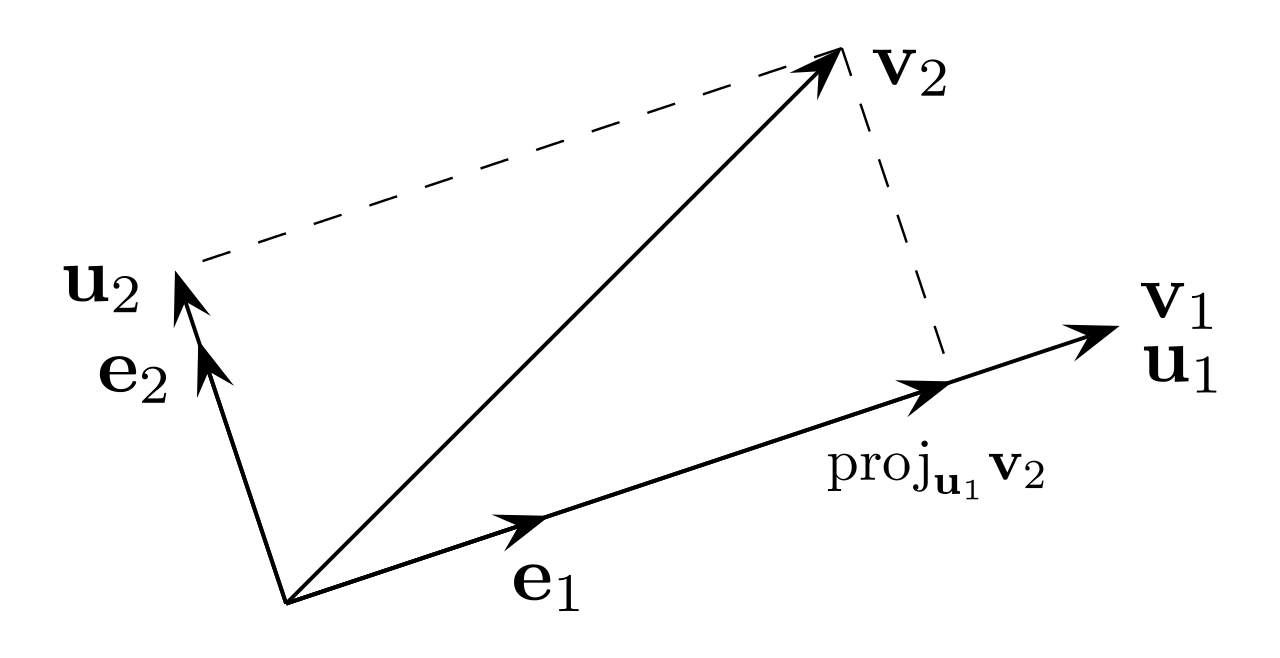
\includegraphics[scale=0.20]{15_6.png}

    \newpage

    \section{Liczby Stirlinga I i II rodzaju i ich interpretacja.}


    \begin{definition}
        \textbf{Liczby Stirling I rodzaju}.

        Dla dowolnego $n \geq 1$ mamy:
        \begin{enumerate}
            \item $c(0,0) = 1$
            \item $c(n,0) = c(0,n) = 0$
            \item $c(n,k) = c(n-1, k-1) + (n-1) * c(n-1, k)$
        \end{enumerate}
        W szczególności:
        \begin{enumerate}
            \item $c(n,n) = 1, c(n,1) = (n-1)!$
            \item $\sum^n_{k=0} c(n,k) = n!$
        \end{enumerate}

        \textbf{Interpretacja}: Przez $c(n,k)$ ($[^n_k]$) oznaczamy liczbę permutacji zbioru n-elementowego, które mają rozkład
        na dokładnie k cykli rozłącznych.
    \end{definition}

    \begin{definition}
        \textbf{Liczby Stirlinga II rodzaju}.

        Dla dowolnego $n \geq 1$ mamy:
        \begin{enumerate}
            \item $S(0,0) = 1$,
            \item $S(n,0) = S(0,n) = 0$,
            \item $S(n,k) = S(n-1, k-1) + k \times S(n-1, k)$.
        \end{enumerate}
        w szczególności  $S(n,n) = S(n,1) = 1$.\\

        \textbf{Interpretacja}: Przez $S(n,k)$ ($\{^n_k\}$) oznaczamy liczbę rozmieszczeń n rozróżnialnych kul na k nierozróżnialnych stosach w taki sposób,
        aby żaden stos nie był pusty.
    \end{definition}


    \newpage

    \section{Twierdzenia Eulera i Fermata; funkcja Eulera.}
    \begin{definition}
        \textbf{Funkcja Eulera (Tocjent)}

        Funkcja przypisująca każdej liczbie naturalnej liczbę liczb względnie pierwszych z nią i nie większych od niej.\newline $\sum_{m|n}^{} \varphi(m) = n$\newline

        \textbf{Własności}
        \begin{enumerate}
            \item $\varphi (n) \leq n - 1$  dla każdego $n>1$
            \item $\varphi (p) \leq p - 1$ dla każdego p będącego liczbą pierwszą
            \item $\varphi (mn) = \varphi (m)\varphi(n)$ jeśli NWD(m,n) = 1 (m i n względnie pierwsze)
            \item $\varphi(p^{k}) = p^{k-1} \cdot (p-1)$ jeśli p jest liczbą pierwszą
            \item $\varphi(n) = n
            \left (  1 - \frac{1}{p_1}\right)
            \left (  1 - \frac{1}{p_2}\right)
            \cdots
            \left (  1 - \frac{1}{p_n}\right)$
            gdzie $p_1, p_2, ..., p_n$ są czynnikami pierwszymi liczby n
            \item jeżeli $n = \prod_{i=1}^{k} p_i^{k_i}$ jest rozkładem liczby n na czynniki pierwsze $\varphi (n) = \prod_{i=1}^{k} \varphi \left( p_i^{k_i} \right )$
        \end{enumerate}
    \end{definition}

    \begin{definition}
        \textbf{Małe Twierdzenie Fermata}

        Jeżeli p jest liczbą pierwszą, to dla dowolnej liczby całkowitej a, liczba $a^{p}-a$ jest podzielna przez p.\newline
        \begin{enumerate}
            \item $a^{p-a} \equiv 0 \pmod p$\newline
        \end{enumerate}

        Jeśli p jest liczbą pierwszą, a a jest taką liczbą całkowitą, że liczby a i p są względnie pierwsze to $a^{p-1} - 1$ dzieli się przez p.\newline

        \begin{enumerate}
            \item$a^{p-1} - 1 \equiv \pmod p$
            \item$a^{p-1} \equiv 1 \pmod p$
        \end{enumerate}

    \end{definition}

    \begin{definition}
        \textbf{Twierdzenie Eulera}

        Jeżeli $m \in \mathbb{Z_{+}}$ oraz $a \in \mathbb{Z}$ są liczbami względnie pierwszymi to m dzieli liczbę $a^{\varphi(m)} - 1$, gdzie $\varphi (m)$ oznacza wartość funkcji Eulera.

        \begin{enumerate}
            \item $a^{\varphi (m)} \equiv 1 \pmod m$\newline
        \end{enumerate}

    \end{definition}
    \newpage

    \section{Konfiguracje i t-konfiguracje kombinatoryczne.}

    \begin{definition}
        \textbf{Konfiuracją kombinatoryczną} $B$ o parametrach $(n,k,r)$ nazywamy rodzinę $k$-elementowych podzbiorów w $X$, jeżeli każdy element $x \in X$ występuje w dokładnie $r$ podbiorach. Zachodzą warunki:
        \begin{enumerate}
            \item $n = |X|$
            \item $|B_i|=k \quad \forall i=1, \dots, b$
            \item $n \cdot r = b \cdot k$ \quad gdzie b to liczba k-elementowych podzbiorów zbioru n-elementowego
        \end{enumerate}
    \end{definition}

    \begin{theorem}
        Istnieje konfiguracja kombinatoryczna $B$ o parametrach $(n, k, r)$ wtedy i tylko wtedy, gdy:
        \begin{enumerate}
            \item $k | n\cdot r$
            \item $\frac{n\cdot r}{k}\leq {n\choose k}$
        \end{enumerate}

    \end{theorem}

    \begin{definition}
        Niech $X$ dowolny zbiór, $|X| = n.$ $B$ rodzina $k-$ podzbiorów $X$ jest
        \textbf{t-konfiguracją kombinatoryczną} o parametrach $(n, k, r_t)$ wtw gdy dla
        każdego $t-$podzbioru $T \subset X$ liczba bloków z $B$ zawierających $T$ jest
        równa $r_t$.
    \end{definition}

    \begin{theorem}
        Jeśli $B$ jest $t$-konfiguracją kombinatoryczną, to
        $B$ jest $s$-konfiguracją kombinatoryczną dla $s = 1, 2,\dots$ $t-1$.
        Uwagi:
        \begin{enumerate}
            \item $r_{t-1}$ $= r_t \cdot \frac{n-t+1}{k-t+1}$
            \item Jeżeli $B$ jest $t-$konfiguracją o parametrach $(n,k,r_t)$, to dla $1 \leq s \leq (t-1)$
            \begin{align*}
                r_s = r_t \cdot \frac{(n-s)(n-s-1)\dots(n-t+1)}{(k-s)(k-s-1)\dots(k-t+1)}
            \end{align*}
            \item Jeśli $B$ jest $t$-konfiguracją o parametrach $(n,k,r_t)$, to
            \begin{align*}
                (k-s)(k-s-1)\dots(k-t+1)|r_t(n-s)(n-s-1)\dots(n-t+1) \\ dla\  0\leq s \leq (t-1)
            \end{align*}
            warunek 3. dla $t\leq 2$ jest konieczny dla istnienia $t$-konfiguracji, ale nie wystarczający
        \end{enumerate}
    \end{theorem}

    \newpage

    \section{Cykl Hamiltona, obwód Eulera, liczba chromatyczna - definicje i twierdzenia.}

    \subsection{Cykl Hamiltona}
    \begin{definition}
        \textbf{Ścieżka Hamiltona}. Ścieżką Hamiltona w grafie $G$ nazywamy ścieżkę, która przechodzi przez wszystkie
        wierzchołki $G$.
    \end{definition}

    \begin{definition}
        \textbf{Cykl Hamiltona}. Powiemy, że graf $G$ ma cykl Hamiltona, jeśli istnieje w nim cykl przechodzący przez
        wszystkie wierzchołki. Taki graf nazwyamy hamiltonowskim.
    \end{definition}

    \begin{theorem}
        Niech $G = (V, E)$ będzie grafem o $n \geq 3$ wierzchołkach. Jeśli dla dwolonych różnych, niesąsiednich
        wierzchołków $u, v \in V$ zachodzi warunek $d(u) + d(v) \geq n$, to G jest hamiltonowski.
    \end{theorem}

    \begin{theorem}
        Jeśli $G$ jest grafem o $n \geq 3$ wierzchołkach w którym minimalny stopień wierzchołka wynosi co najmniej
        $\frac{n}{2}$, to G jest hamiltonowski.
    \end{theorem}

    \begin{theorem}
        Niech $G = (V, E)$ będzie grafem o $n \geq 2$ wierzchołkach i takim, że $d(u) + d(v) \geq n-1$ dla dwóch dowolnych
        różnych, niesąsiednich wierzchołków $u, v \in V$. Wtedy G ma ścieżkę hamiltona.
    \end{theorem}

    \subsection{Obwód Eulera}
    \begin{definition}
        \textbf{Droga Eulera}. Drogą Eulera w grafie $G$ nazywamy drogę $v_1, v_2, \dots, v_m$, w której każda krawędź grafu G użyta
        jest dokładnie raz.
    \end{definition}
    \begin{definition}
        \textbf{Obwód Eulera}. Jeśli w grafie $G$ istnieje droga Eulera, w której pierwszy i ostatni wierzchołek są identyczne, to nazywamy ją
        obwodem Eulera. Graf ten nazywamy wtedy eulerowskim.
    \end{definition}

    \begin{theorem}
        Niech $G$ będzie grafem spójnym. Wówczas następujące warunki są równowaźne:
        \begin{enumerate}
            \item G jest grafem eurelowskim,
            \item stopień każdego wierzchołka w G jest parzysty.
        \end{enumerate}
    \end{theorem}

    \begin{theorem}
        Niech G będzie grafem spójnym. Wówczas G ma drogę Eulera $\Leftrightarrow$ w G są dokładnie zero lub dwa wierzchołki
        stopnia nieparzystego.
    \end{theorem}

    \subsection{Liczba chromatyczna}
    \begin{definition}
        \textbf{Kolorowanie wierchołkowe}. Kolorowaniem wierzchołkowym grafu $G = (V, E)$ przy użyciu (co najwyżej) $k$
        kolorów nazywamy funkcję $c: V \rightarrow \{1, \dots, k\}$ spełniającą warunek
        $c(u) \neq c(v) ~~ \forall u, v \in V : uv \in E$.
    \end{definition}

    \begin{definition}
        \textbf{Liczba chromatyczna}. Liczbą chromatyczną grafu G nazywamy najmniejszą liczbę $k \in \mathbb{N}$, dla
        której istnieje kolorwanie wierzchołkowe G przy użyciu k kolorów. Oznaczamy $\chi(G)$.
        \begin{enumerate}
            \item $\chi(G) = 1 \Leftrightarrow |E(G)| = 0$
            \item $\chi(T) = 2$ dla każdego drzewa T o przynajmniej dwóch wierzchołkach
            \item $\chi(C_{2k}) = 2, \chi(C_{2k+1}) = 3$
            \item $\chi(K_n) = n$
        \end{enumerate}
    \end{definition}

    \begin{theorem}
        Niech G będzie dowolnym grafem. Wtedy $\chi(G) \leq d_{max}(G) + 1$.
    \end{theorem}

    \begin{theorem}
        Niech G będzie grafem spójnym. Wówczas $\chi(G) \leq d_{max}(G)$, o ile G nie jest grafem pełnym ani cyklem o
        nieparzystej liczbie wierzchołków.
    \end{theorem}

    \newpage

    \section{Algorytm Forda-Fulkersona wyznaczania maksymalnego przepływu.}

    \begin{definition}
        \textbf{Siecią przepływową} nazywamy zestaw $(V, \vec{E}, s, t, c)$, gdzie $(V, \vec{E})$ jest grafem
        skierowanym wraz z wyróżnionymi wierzchołkami $s$ - \textbf{źródłem} i $t$ - \textbf{ujściem} oraz
        \textbf{funkcją pojemności krawędzi} $c: ~ \vec{E} \rightarrow \mathbb{R}$.
    \end{definition}

    \begin{definition}
        \textbf{Przepływem} w sieci $(V, \vec{E}, s, t, c)$ nazywamy funkcję $f: \vec{E} \rightarrow \mathbb{R}$
        spełniającą następujące warunki:
        \begin{enumerate}
            \item $f(\vec{uv}) \leq c(\vec{uv})$  dla każdej krawędzi $\vec{uv} \in \vec{E}$,
            \item dla każdego ustalonego $v \in V\ \{s, t\}:$
            \begin{align*}
                \sum_{\vec{uv} \in \vec{E}} ~ f(\vec{uv}) ~~ = ~~ \sum_{\vec{vw} \in \vec{E}} ~ f(\vec{vw}).
            \end{align*}
        \end{enumerate}
        Liczbę $|f| =  \sum_{\vec{su}  \in \vec{E}} f(\vec{su}) = \sum_{\vec{wt} \in \vec{E}} f(\vec{wt})$ nazywamy
        \textbf{wartością przepływu} f.\\

        Przepływ f nazywamy \textbf{maksymalnym}, jeśli jego wartość jest największa spośród wszystkich przepływów w
        danej sieci.
    \end{definition}

    \begin{definition}
        Niech $(V, \vec{E}, s, t, c)$ będzie siecią przepływową oraz $f$ pewnym przepływem tej sieci. \textbf{Siecią rezydualną}
        nazywamy sieć $G_f = (V, E_f, s, t, c_f)$, gdzie $E_f = \vec{E} \cup \{\vec{vu}: \vec{uv} \in \vec{E}\}$ z funkcją
        pojemności określoną wzorem:
        \begin{align*}
            c_f(\vec{uv}) = c(\vec{uv}) - f(\vec{uv}) ~~ \text{dla} ~ \vec{uv} \in  \vec{E} ~  \text{t. że} ~ c(\vec{uv}) > 0
        \end{align*}
        \begin{align*}
            c_f(\vec{uv}) = f(\vec{uv}) ~~ \text{dla} ~ \vec{uv} \notin  \vec{E} ~  \text{t. że} ~ \vec{vu} \in \vec{E} \text{i} f(\vec{uv}) > 0
        \end{align*}
        oraz $c_f(\vec{uv}) = 0$ w pozostałych przypadkach.
    \end{definition}

    \begin{definition}
        \textbf{Ścieżką rozszerzającą} dla przepływu f nazywamy dowolną ścieżkę (skierowaną) $v_0 \rightarrow v_1 \rightarrow \cdots \rightarrow v_k$
        w sieci rezydualnej $G_f$ łączącą wierzchołki $v_0 = s$ i $v_k = t$, w której $c_f(\vec{v_i v_{i+1}}) > 0$ dla
        każdego $i = 0, \cdots, k-1$.
    \end{definition}

    \begin{theorem}
        \textbf{Algorytm Forda-Fulkersona}. W celu znalezienia maksymalnego przepływu $f$ w sieci przepływowej
        $(V, \vec{E}, s, t, c)$:
        \begin{enumerate}
            \item przyjmujemy początkowo dowolny (np. zerowy) przepływ $f$,
            \item budujemy sieć rezydualną $G_f$,
            \item dopóki w $G_f$ istnieje ścieżka rozszerzająca $P = v_0 \rightarrow v_1 \rightarrow \cdots \rightarrow v_k$
            określamy $c_p = min_{i = 0, \cdots, k-1} c_f(\vec{v_i v_{i+1}})$, a następni zwiększamy o $c_p$ wartość
            przepływu $f$ na krawędziach $\vec{v_i v_{i+1}}$ tej ścieżki i uaktualniamy wartośi funkcji $c_f$ sieci
            rezydualnej.
        \end{enumerate}
    \end{theorem}

    \begin{definition}
        \textbf{Przekrojem} w sieci przepływowej $(V, \vec{E}, s, t, c)$ nazywamy parę zbiorów $(S, T)$ spełniającą
        warunki:
        \begin{enumerate}
            \item $S \cup T = V$,
            \item $S \cap T = \emptyset$,
            \item $s \in S, t \in T$.
        \end{enumerate}

        \textbf{Pojemnością} przekroju $(S,T)$ nazywamy liczbę
        \begin{align*}
            c(S, T) = \sum_{(u,v) \in \vec{E} \cap (S \times T)} c(\vec{uv}).
        \end{align*}
    \end{definition}

    \begin{theorem}
        Niech $(V, \vec{E}, s, t, c)$ będzie siecią przepływową. Wówczas \textbf{maksymalna wartość przepływu jest
        jest równa minimalnej pojemności} przekroju w tej sieci.
    \end{theorem}

    \newpage

    \section{Rozwiązywanie równań rekurencyjnych przy użyciu funkcji tworzących (generujących) oraz przy użyciu
    równania charakterystycznego.}

    \begin{definition}
        \textbf{Liniowym równaniem rekurencyjnym rzędu r} (o stałych współczynnikach) nazywamy równanie postaci:
        \begin{align*}
            x_{n+r} = c_1 x_{n+r-1} +  \cdots + c_r x_n + f(n)
        \end{align*}
        w którym $c_i  \in \mathbb{R}, c_r \neq 0$  oraz $f:  \mathbb{N} \rightarrow \mathbb{R}$ jest dowolną funkcją.
        Jeśli funkcja f jest stale równa zero, to powyższe równanie nazywamy \textbf{jednorodnym}.
    \end{definition}

    \begin{definition}
        \textbf{Rozwiązaniem szczególnym} równania nazywamy dowolny ciąg $(x_n)$ spełniający zależność rekurencyjną.
        Dla każdego równania jednorodnego rozwiązanie szczególnym jest ciąg stały równy zero.

        \textbf{Rozwiązaniem ogólnym} równania nazywamy wzór ogólny (zależny od pewnych parametrów) pozwalający
        wyznaczyć wszystkie rozwiązania szczególne.
    \end{definition}

    \subsection{Funkcje tworzące.}
    \begin{definition}
        \textbf{Funkcją tworzącą} (generujacą) ciągu $(a_n)$ nazywamy szereg
        \begin{align*}
            \sum_{n=0}^{\infty} a_n x^n.
        \end{align*}
        Jest to tylko inny zapis ciągu (wyraz $a_n$ to współczynnik przy $x^n$) - nie interesują nas kwestie zbieżności,
        podstawiania wartości za x, ciągłości/różniczkowalności funkcji określonej takim szeregiem itd.

        Jeżeli jednak funkcja tworząca pewnego ciągu "wygląda" jak zbieżny szereg określający funkcję znaną z analizy
        to możemy używać skróconego zapisu, np. $\sum_{n=0}^{\infty} \frac{1}{n!} x^n = e^x$.
    \end{definition}

    \begin{theorem}
        \textbf{Operacje na funkcjach tworzących}.
        \begin{enumerate}
            \item Funkcje tworzące można \textbf{dodawać,odejmować i mnożyć przez liczbę} - odpowiadają temu operacje
            dodawania, odejmowania i mnożenia przez liczbę wyrazów ciągu.
            \item \textbf{Mnożeniu dwóch funkcji tworzących} odpowiada operacja "splotu", tzn. jeśli
            $A(x) =  \sum_{n=0}^{\infty} a_n x^n$ i $B(x) = \sum_{n=0}^{\infty} b_n x^n$, to
            $A(x) * B(x) = \sum_{n=0}^{\infty} c_n x^n$, gdzie $c_n = \sum_{k=0}^n a_k b_{n-k}$.
            \item Jeśli funkcja tworząca A(x) ma "element odwrotny", tzn. taką funkcję tworzącą B(x) dla której
            $A(x) * B(x) = 1$, to mówimy że A(x) jest \textbf{odwracalna} i piszemy $\frac{1}{A(x)} = B(x)$.
            \item \textbf{Mnożeniu funkcji} tworzącej \textbf{przez x} odpowiada przesunięcie ciągu (dopisanie na początek
            wyrazu zerowego). Operajcją odwrotną jest odjęcie wyrazu zerowego i podzielenie przez x.
            \item Funkcje tworzące można \textbf{różniczkować} według wzoru:
            \begin{align*}
                (\sum_{n=0}^{\infty} a_n x^n)' = \sum_{n=1}^{\infty} n a_n x^{n-1} = \sum_{n=0}^{\infty} (n+1) a_{n+1} x^n
            \end{align*}
            \item Zachodzą wzory na \textbf{pochodne} znane z analizy, np. $(A(x) * B(x))' = A'(x)B(x) + A(x)B'(x)$.
            \item Operacja \textbf{"całkowania"} (odwrotna do różniczkowania):
            \begin{align*}
                \int (\sum_{n=0}^{\infty} a_n x^n) = \sum_{n=0}^{\infty} \frac{a_n}{n+1} x^{n+1} = \sum_{n=0}^{\infty} \frac{a_n - 1}{n} x^n
            \end{align*}
            Wyraz $a_n$ można "odzyskać" z funkcji tworzącej A(x) wykonując jej n-krotne różniczkowanie.
        \end{enumerate}
    \end{theorem}

    \begin{theorem}
        Dla dowolnej liczby naturalnej $m \geq 1$ zachodzi wzór:
        \begin{align*}
            \frac{1}{(1-x)^m} ~ = ~ \sum_{n=0}^{\infty} \binom{n+m-1}{n} x^n.
        \end{align*}

        Dla dowolneego $\alpha \in \mathbb{R}$ oraz $|x| < 1$ zachodzi wzór:
        \begin{align*}
            (1+x)^{\alpha} ~ - ~ \sum_{n=0}^{\infty} \binom{\alpha}{n} x^n
        \end{align*}
    \end{theorem}

    \subsection{Równanie charakterystyczne.}
    \begin{definition}
        \textbf{Równanie charakterystyczne} równania rekurencyjnego. Weźmy równanie rekurencyjne jednorodne
        \begin{align*}
            a_n = A a_{n-1} + B a_{n-2}
        \end{align*}
        gdzie dane są współczynniki A, B. Załóżmy, że ma ono rozwiązanie postaci $a_n = t^n$. Podstawiając otrzymujemy:
        \begin{align*}
            t^n = A t^{n-1} + B t^{n-2}.
        \end{align*}
        Dzielimy obie strony przez $t^{n-2}$:
        \begin{align*}
            t^2 = A t^1 + B
        \end{align*}
        \begin{align*}
            t^2 - A t^1 - B = 0.
        \end{align*}
        Równanie to nazywamy równaniem charakterystycznym równania rekurencyjnego. W tym przypadku jest to równanie kwadratowe.

        Jeżeli nie ma ono pierwiastków podwójnych, wówczas:
        \begin{align*}
            a_n = C r_1^n + D r_2^n.
        \end{align*}
        Jeżeli ma pierwiastki podwójne, to:
        \begin{align*}
            a_n = (C + Dn) r_1^n.
        \end{align*}
        C i D są dowolnymi stałymi a $r_{1}$ i $r_{2}$ są pierwiastkami równania charakterystycznego. Jeżeli dane jest
        $a_{1}$ i $a_{2}$ wówczas można łatwo ułożyć układ równań i otrzymać ich wartość.
    \end{definition}

    \newpage

    \section{Ciąg i granica ciągu liczbowego, granica funkcji.}

    \subsection{Ciągi.}

    \begin{definition}
        \textbf{Ciąg liczbowy}. Ciągiem liczbowym nazywamy funkcję $\mathbb{N} \rightarrow \mathbb{R}$. Wartość tej
        funkcji dla liczby naturalnej $n$ nazywamy $n$-tym wyrazem ciągu i oznaczamy przez $a_n$, $b_n$ itp. Ciągi o
        takich wyrazachoznaczamy odpowiednio przez $(a_n)$, $(b_n)$  itp. Zbiór wyrazów ciągu $(a_n)$, tj.
        $\{a_n : n  \in \mathbb{N}\}$ oznaczamy krótko przez  $\{a_n\}$.
    \end{definition}

    \begin{definition}
        \textbf{Granica właściwa ciągu}. Ciąg $(a_n)$ jest zbieżny do granicy właściwej $a \in \mathbb{R}$, co zapisujemy:
        \begin{align*}
            lim_{n  \rightarrow \infty} ~ a_n = a
        \end{align*}
        wtedy i tylko wtedy, gdy
        \begin{align*}
            \forall \varepsilon > 0 ~~ \exists  n_0 \in \mathbb{N} ~~ \forall n \in \mathbb{N} ~~~ [(n > n_0) \Rightarrow (|a_n - a| < \varepsilon)]
        \end{align*}
    \end{definition}

    \begin{definition}
        \textbf{Granice niewłaściwe ciągu}.

        Ciąg $(a_n)$ jest zbieżny do granicy niewłaściwej $\infty$, co zapisujemy:
        \begin{align*}
            lim_{n \rightarrow \infty} ~ a_n = \infty
        \end{align*}
        wtedy i tylko wtedy, gdy:
        \begin{align*}
            \forall \varepsilon > 0 ~~ \exists  n_0 \in \mathbb{N} ~~ \forall n \in \mathbb{N} ~~~ [(n > n_0) \Rightarrow (a_n > \varepsilon)]
        \end{align*}

        Ciąg $(a_n)$ jest zbieżny do granicy niewłaściwej $-\infty$, co zapisujemy:
        \begin{align*}
            lim_{n \rightarrow \infty} a_n = -\infty
        \end{align*}
        wtedy i tylko wtedy, gdy:
        \begin{align*}
            \forall \varepsilon < 0 ~~ \exists  n_0 \in \mathbb{N} ~~ \forall n \in \mathbb{N} ~~~ [(n > n_0) \Rightarrow (a_n < \varepsilon)]
        \end{align*}
    \end{definition}

    \begin{theorem}
        \textbf{O ograniczoności ciągu zbieżnego}. Jeśli ciąg jest zbieżny do granicy właściwej, to jest ograniczony.
    \end{theorem}

    \begin{theorem}
        \textbf{O równoważności granic.}
        \begin{align*}
            lim_{n \rightarrow \infty} ~ a_n = 0 ~~ \Leftrightarrow ~~ lim_{n \rightarrow \infty} ~ |a_n| = 0.
        \end{align*}
    \end{theorem}

    \begin{theorem}
        \textbf{O dwóch ciągach}. Jeśli ciągi $(a_n)$, $(b_n)$ spełniają warunki:
        \begin{enumerate}
            \item $a_n \leq b_n ~~~ \forall n \geq n_0$
            \item $lim_{n \rightarrow \infty} a_n = \infty$
        \end{enumerate}
        to
        \begin{align*}
            lim_{n \rightarrow \infty} ~ b_n = \infty.
        \end{align*}

        Prawdziwe jest także analogiczne twierdzenie dla ciągów zbieżnych do granicy niewłaściwej $-\infty$.
    \end{theorem}

    \begin{theorem}
        \textbf{O trzech ciągach}. Jeśli ciągi $(a_n)$, $(b_n)$, $(c_n)$ spełniają warunki:
        \begin{enumerate}
            \item $a_n \leq b_n \leq c_n ~~~ \forall n \geq n_0$
            \item $lim_{n  \rightarrow \infty} a_n = lim_{n \rightarrow \infty} c_n = b$
        \end{enumerate}
        to
        \begin{align*}
            lim_{n \rightarrow \infty} ~ b_n = b.
        \end{align*}
    \end{theorem}

    \begin{theorem}
        \textbf{O ciągu monotonicznym i ograniczonym}. Jeżeli ciąg $(a_n)$ jest niemalejący dla $n \geq n_0$ oraz
        ograniczony z góry, to jest zbieżny do granicy właściwej $sup\{a_n : n \geq n_0\}$.

        Prawdziwe jest także analogiczne twierdzenie dla ciągu nierosnącego i ograniczonego z dołu.
    \end{theorem}

    \subsection{Funkcje.}

    \begin{definition}
        \textbf{Heinego granicy właściwej funkcji w punkcie}. Niech $x_0 \in \mathbb{R}$ oraz niech funkcja $f$ będzie
        określona przynajmniej na sąsiedztwie $S(x_0)$. Liczba $g$ jest granicą właściwą funkcji $f$ w punkcie $x_0$, co
        zapisujemy
        \begin{align*}
            lim_{x \rightarrow x_0} ~ f(x) = g
        \end{align*}
        wtedy i tylko wtedy, gdy
        \begin{align*}
            \forall_{(x_n): ~ \{x_n\} \subset S(x_0)} ~~ [(lim_{n \rightarrow \infty} x_n = x_0) \Rightarrow (lim_{n \rightarrow \infty} f(x_n) = g)].
        \end{align*}
    \end{definition}

    \begin{definition}
        \textbf{Cauchy'ego granicy właściwej funkcji w punkcie}. Niech $x_0 \in \mathbb{R}$ oraz niech funkcja $f$ będzie
        określona przynajmniej na sąsiedztwie $S(x_0)$. Liczba $g$ jest granicą właściwą funkcji $f$ w punkcie  $x_0$,
        co zapisujemy
        \begin{align*}
            lim_{x \rightarrow x_0} ~ f(x)  = g
        \end{align*}
        wtedy i tylko wtedy, gdy
        \begin{align*}
            \forall \varepsilon > 0 ~~ \exists \delta > 0 ~~ \forall  x \in S(x_0)  ~~~ [(|x - x_0| <  \delta) \Rightarrow (|f(x) - g| < \varepsilon)].
        \end{align*}
        \hfill \\

        Funkcja $f$ ma granicę niewłaściwą $\infty$ w punkcie $x_0$ wtedy i tylko wtedy, gdy
        \begin{align*}
            \forall \varepsilon > 0 ~~ \exists \delta > 0 ~~ \forall  x \in S(x_0)  ~~~ [(|x - x_0| <  \delta) \Rightarrow (f(x) > \varepsilon)].
        \end{align*}

    \end{definition}

    \begin{theorem}
        \textbf{O nieistnieniu granicy funkcji w punkcie}. Jeśli istnieją ciągi $(x'_n)$, $(x''_n)$ spełniające warunki:
        \begin{enumerate}
            \item $lim_{n \rightarrow \infty} x'_n = x_0$, przy czym $x'_n \neq x_0 ~~ \forall n \in \mathbb{N}$
            oraz $lim_{n \rightarrow \infty}  ~ f(x'_n) = g'$,
            \item $lim_{n \rightarrow \infty} x''_n = x_0$, przy czym $x''_n \neq x_0 ~~ \forall n \in \mathbb{N}$
            oraz $lim_{n \rightarrow \infty}  ~ f(x''_n) = g''$,
            \item $g' \neq g''$,
        \end{enumerate}
        to granica $lim_{x \rightarrow x_0} ~ f(x)$ nie istnieje (właściwa ani niewłaściwa).
    \end{theorem}

    \begin{theorem}
        \textbf{Warunek konieczny i wystarczajacy istnienia granicy}. Funckja $f$ ma w punkcie $x_0$ granicę
        właściwą (niewłaściwą) wtedy i tylko wtedy, gdy
        \begin{align*}
            lim_{x \rightarrow x^{-}_0}  ~ f(x) ~ = ~ lim_{x \rightarrow x^{+}_0}  ~ f(x)
        \end{align*}
        Wspólna wartość granic jednostronnych jest wtedy granicą funkcji.
    \end{theorem}

    \begin{theorem}
        \textbf{O niesitnieniu granicy funkcji w nieskończoności}. Jeżeli istnieją ciągi $(x'_n)$, $(x''_n)$
        spełniające warunki:
        \begin{enumerate}
            \item $lim_{n \rightarrow \infty} ~ x'_n = \infty $ oraz $ lim_{n \rightarrow \infty} ~ f(x'_n) = g'$,
            \item $lim_{n \rightarrow \infty} ~ x''_n = \infty $ oraz $ lim_{n \rightarrow \infty} ~ f(x''_n) = g''$,
            \item $g' \neq g''$,
        \end{enumerate}
        to nie istnieeje granica $lim_{x \rightarrow x_0} ~ f(x)$ (właściwa ani niewłaściwa).
    \end{theorem}

    \begin{theorem}
        \textbf{O dwóch funkcjach}. Jeśli funkcje $f$ i $g$ spełniają warunki:
        \begin{enumerate}
            \item $f(x) \leq g(x) ~~ \forall x \in S(x_0)$,
            \item $lim_{x \rightarrow x_0} ~ f(x) = \infty$,
        \end{enumerate}
        to
        \begin{align*}
            lim_{x \infty x_0} ~ g(x) = \infty.
        \end{align*}
    \end{theorem}

    \begin{theorem}
        \textbf{Granice specjalne}
        \setlength{\jot}{10pt}
        \begin{align*}
            &\lim_{x \to +\infty} a^{x} x^{\alpha} \stackrel{[0 \cdot \infty]}{=}  \text{0 dla a} \in (0, 1), \alpha \geq 0 \\
            &\lim_{x \to 0} \frac{\sin{x}}{x} \stackrel{[\frac{0}{0}]}{=} \text{1 oraz}    \lim_{x \to 0} \frac{\arcsin{x}}{x} \stackrel{[\frac{0}{0}]}{=} 1\\
            &\lim_{x \to 0} (1 + x)^{\frac{1}{x}} \stackrel{1^{\infty}}{=} \text{e oraz}   \lim_{x \to \infty} (1 + x)^{\frac{1}{x}} \stackrel{\infty^{0}}{=} 1 \\
            &\lim_{x \to 0} \frac{a^x -1}{x} \stackrel{[\frac{0}{0}]}{=} \ln{a} \text{ dla a $>$ 0, w szczególności } \lim_{x \to 0} \frac{e^x -1}{x} \stackrel{[\frac{0}{0}]}{=} 1 \\
            &\lim_{x \to 0} \frac{\log_{a}(1 + x)}{x} \stackrel{[\frac{0}{0}]}{=} \frac{1}{\ln{a}} \text{, w szczególności } \lim_{x \to 0} \frac{\ln(1 + x)}{x} \stackrel{[\frac{0}{0}]}{=} 1 \\
            &\lim_{x \to \pm \infty} (1 + \frac{a}{x})^{x} \stackrel{[1^{\infty}]}{=} e^{a} \text{, dla a} \in \mathbb{R} \\
            &\lim_{x \to 0} \frac{(1 + x)^a - 1}{x} \stackrel{[\frac{0}{0}]}{=} \text{a, dla a} \in \mathbb{R}
        \end{align*}
    \end{theorem}

    \begin{theorem}
        \textbf{Reguła de L'Hostpiala}. Jeżeli funkcja $f$ i  $g$ spełniają warunki:
        \begin{enumerate}
            \item $lim_{x \rightarrow x_0} f(x) = lim_{x \rightarrow x_0} g(x) = 0 ~~ (\infty)$, przy czym $g(x) \neq 0$ dla $x \in S(x_0)$
            \item istnieje granica $lim_{x \rightarrow x_0} \frac{f'(x)}{g'(x)}$ (właściwa lub niewłaściwa),
        \end{enumerate}
        to
        \begin{align*}
            lim_{x \rightarrow x_0} \frac{f(x)}{g(x)} = lim_{x \rightarrow x_0} \frac{f'(x)}{g'(x)}
        \end{align*}
    \end{theorem}

    \newpage

    \section{Ciągłość i pochodna funkcji. Definicja i podstawowe twierdzenia.}

    \subsection{Ciągłość.}

    \begin{definition}
        \textbf{Funkcja ciągła w punkcie}. Niech $x_0 \in \mathbb{R}$ oraz niech funkcja $f$ będzie określona przynajmniej
        na otoczeniu $O(x_0)$. Funkcja $f$ jest ciągła w ounkcie $x_0$ wtedy i tylko wtedy, gdy
        \begin{align*}
            lim_{x \rightarrow x_0} ~ f(x) = f(x_0).
        \end{align*}
        \hfill \\

        \textbf{Funkcja jest ciągła na zbiorze}, jeżeli jest ciągła w każdym punkcie tego zbioru.
    \end{definition}

    \begin{theorem}
        \textbf{Warunek konieczny i wystarczający ciągłości funkcji}. Funckja jest ciągła w punkcie wtedy i tylko wtedy,
        gdy jest w tym punkcie ciągła lewostronnie i prawostronnie.
    \end{theorem}

    \begin{definition}
        \textbf{Nieciągłość funkcji}. Niech $x_0 \in \mathbb{R}$ oraz niech funkcja $f$ będzie określona przynajmniej
        na otoczeniu $O(x_0)$. Funkcja $f$ jest nieciągła w punkcie $x_0$ wtedy i tylko wtedy, gdy nie istnieje
        granica $lim_{x \rightarrow x_0} ~ f(x)$ albo gdy $lim_{x \rightarrow x_0} ~ f(x) \neq f(x_0)$.
        \hfill \\

        \textbf{Nieciągłość pierwszego rodzaju}. Jeżeli istnieją granice skończone $lim_{x \rightarrow x^{-}_0 ~ f(x)}$,
        $lim_{x \rightarrow x^{+}_0} ~ f(x)$ oraz
        \begin{align*}
            lim_{x \rightarrow x^{-}_0} ~ f(x) \neq  f(x_0) ~~~ \text{lub} ~~~ lim_{x \rightarrow x^{+}_0} ~ f(x) \neq f(x_0).
        \end{align*}
        Mówimy, że funkcja $f$ ma w punkcie $x_0$ nieciągłość pierwszego rodzaju typu "skok", jeżeli spełnia warunek
        \begin{align*}
            lim_{x \rightarrow x^{-}_0} ~ f(x) ~ \neq ~ lim_{x \rightarrow x^{+}_0} ~ f(x).
        \end{align*}
        Mówi, że funkcja $f$ ma w punkcie $x_0$ nieciągłość pierwszego rodzaju typu "luka", jeżeli spełnia warunek
        \begin{align*}
            lim_{x \rightarrow x^{-}_0} ~ f(x) ~ = ~ lim_{x \rightarrow x^{+}_0} ~ f(x) ~ \neq ~ f(x_0).
        \end{align*}
        \hfill \\

        \textbf{Nieciągłość drugiego rodzaju}. Jeżeli co najmniej jedna z granic
        \begin{align*}
            lim_{x \rightarrow x^{-}_0} ~ f(x), ~~ lim_{x \rightarrow x^{+}_0} ~ f(x)
        \end{align*}
        nie istnieje lub jest niewłaściwa.
    \end{definition}

    \begin{theorem}
        \textbf{Weierstrassa o ograniczoności funkcji ciągłej}. Jeżeli funkcja jest ciągła na przedziale domkniętym
        i ograniczonym, to jest na nim ograniczona.
    \end{theorem}

    \begin{theorem}
        \textbf{Weierstrassa o osiąganiu kresów}. Jeżeli funkcja $f$ jest ciągła na przedziale domkniętym $[a, b]$,to
        \begin{align*}
            \exists c \in [a,b] ~~ f(c) = ~ inf_{x \in [a,b]} ~ f(x) ~~ \text{oraz} ~~ \exists d \in [a,b] ~~ f(d) = ~ sup_{x \in [a,b]} ~ f(x)
        \end{align*}
    \end{theorem}

    \begin{theorem}
        \textbf{Darboux o przyjmowaniu wartości pośrednich}. Jeżeli funkcja $f$ jest ciągła na przedziale $[a,b]$ oraz
        spełnia warunek $f(a) < f(b)$, to
        \begin{align*}
            \forall w \in (f(a, f(b))) ~ \exists c \in (a,b) ~~ f(c) = w.
        \end{align*}
    \end{theorem}


    \subsection{Pochodna.}

    \begin{definition}
        \textbf{Iloraz różnicowy}. Niech  $x_0 \in \mathbb{R}$ oraz niech funkcja $f$ będzie określona przynajmniej
        na otoczeniu $O(x_0, r)$, gdzie $r > 0$. Ilorazem różnicowym funkcji $f$ w punkcie $x_0$  odpowiadającym przyrostowi
        $\Delta x$, gdzie $0 < |\Delta x| < r$, zmiennej niezależnej nazywamy liczbę
        \begin{align*}
            \frac{\Delta f}{\Delta x} \stackrel{def}{=} \frac{f(x_0 + \Delta x) - f(x_0)}{\Delta x}
        \end{align*}
    \end{definition}

    \begin{definition}
        \textbf{Pochodna właściwa funkcji}. Niech $x_0 \in \mathbb{R}$ oraz niech funkcja $f$ będzie określona przynajmniej
        na otoczeniu $O(x_0)$. Pochodną właściwą funkcji $f$ w punkcie $x_0$ nazywamy granicę właściwą
        \begin{align*}
            f'(x_0) ~ \stackrel{def}{=} ~ lim_{x \rightarrow x_0} ~ \frac{f(x) - f(x_0)}{x - x_0}
        \end{align*}

        Inaczej mówiąc pochodna funkcji $f$ jest granicą ilorazu różnicowego gdy $\Delta x \rightarrow \infty$. Mamy zatem
        \begin{align*}
            f'(x_0) ~ \stackrel{def}{=} ~ lim_{\Delta x \rightarrow \infty} ~ \frac{f(x_0 + \Delta x) - f(x_0)}{\Delta x}
        \end{align*}
    \end{definition}

    \begin{theorem}
        \textbf{Warunek konieczny istnienia pochodnej właściwej funkcji}. Jeżeli funkcja ma pochodną właściwą w punkcie,
        to jest ciągła w tym punkcie. Implikacja odwrotna nie jest prawdziwa.
    \end{theorem}

    \begin{definition}
        \textbf{Pochodne jednostronne właściwe funkcji}. Niech $x_0 \in \mathbb{R}$ oraz niech funkcja $f$ będzie
        określona przynajmniej na otoczeniu  $O(x^{-}_0)$. Pochodną lewostronną właściwą funkcji $f$ w punkcie $x_0$
        nazywamy granicę właściwą
        \begin{align*}
            f'_{-}(x_0) ~ \stackrel{def}{=} ~ lim_{x \rightarrow x^{-}_0} ~ \frac{f(x) - f(x_0)}{x - x_0}
        \end{align*}
        Analogicznie definiujemy $f'_{+}(x_0)$.\\

        Jeżeli funkcja ma w punkcie pochodną lewostronną (prawostronną) właściwą, to jest w nim ciągła lewostronnie
        (prawostronnie).
    \end{definition}

    \begin{definition}
        \textbf{Pochodna funkcji na zbiorze}. Funkcja ma pochodną właściwą na zbiorze wtedy i tylko wtedy, gdy ma pochodną
        właściwą w każdym punkcie tego zbioru.
    \end{definition}

    \begin{definition}
        \textbf{Pochodna niewłaściwa funkcji}. Niech $f$ będzie funkcją ciągłą w punkcie $x_0 \in \mathbb{R}$. Funkcja
        $f$ ma w punkcie $x_0$ pochodną niewłaściwą wtedy i tylko wtedy, gdy
        \begin{align*}
            lim_{x \rightarrow  x_0} ~ \frac{f(x) - f(x_0)}{x - x_0} = \infty ~~ \text{albo} ~~ lim_{x  \rightarrow x_0} ~ \frac{f(x) - f(x_0)}{x - x_0} = -\infty
        \end{align*}
        Podobnie definiujemy pochodne niewłaściwe jednostronne.
    \end{definition}

    \begin{theorem}
        \textbf{Zastosowanie różniczki do obliczeń przybliżonych}. Jeżeli funkcja $f$ ma pochodną właściwą w punkcie
        $x_0$, to
        \begin{align*}
            f(x_0 + \Delta x) \approx f(x_0) + f'(x_0)\Delta x
        \end{align*}
        Przy czym błąd, jaki popełniamy zastępując przyrost funkcji
        \begin{align*}
            \Delta f = f(x_0 \Delta x) - f(x_0)
        \end{align*}
        jej różniczką $df = f'(x_0)\Delta x$, dąży szybciej do zera niż przyrost zmiennej niezależnej $\Delta x$, tzn.
        \begin{align*}
            lim_{\Delta  x  \rightarrow 0} \frac{\Delta f - df}{\Delta  x} = 0.
        \end{align*}
    \end{theorem}

    \begin{theorem}
        \textbf{Rolle'a}. Jeśli funkcja $f$ spełnia warunki:
        \begin{enumerate}
            \item jest ciągła na $[a,b]$
            \item ma pochodną właściwą lub niewłaściwą na $(a,b)$,
            \item $f(a) = f(b)$,
        \end{enumerate}
        to istnieje punkt $c \in (a,b)$ taki, że:
        \begin{align*}
            f'(c) = 0.
        \end{align*}
    \end{theorem}

    \begin{theorem}
        \textbf{Lagrange'a}. Jeżeli funkcja $f$ spełnia warunki:
        \begin{enumerate}
            \item jest ciągła na $[a,b]$,
            \item ma pochodną właściwą lub niewłaściwą na $(a,b)$,
        \end{enumerate}
        to istnieje punkt $c \in (a,b)$ taki, że
        \begin{align*}
            f'(c) = \frac{f(b)-f(a)}{b-a}
        \end{align*}
    \end{theorem}

    \newpage

    \section{Ekstrema funkcji jednej zmiennej. Definicje i twierdzenia.}

    \begin{definition}
        \textbf{Minimum lokalne funkcji}. Funkcja $f$ ma w punkcie $x_0 \in \mathbb{R}$ minimum lokalne, jeżeli:
        \begin{align*}
            \exists \delta > 0 ~ \forall x \in S(x_0, \delta) ~~ f(x) \geq f(x_0).
        \end{align*}
        Analogicznie definiujemy \textbf{maksimum lokalne}.\\

        \textbf{Minimum lokalne jest właściwe}, jeżeli:
        \begin{align*}
            \exists \delta > 0 ~ \forall x \in S(x_0, \delta) ~~ f(x) > f(x_0).
        \end{align*}
        Analogicznie definiujemy \textbf{maksimum lokalne właściwe}.\\
    \end{definition}

    \begin{theorem}
        \textbf{Fermata, warunek konieczny istnienia ekstremum}. Jeżeli funkcja $f$ ma:
        \begin{enumerate}
            \item esktremum lokalne w punkcie $x_0$,
            \item pochodną $f'(x_0)$,
        \end{enumerate}
        to
        \begin{align*}
            f'(x_0) = 0.
        \end{align*}
    \end{theorem}

    \begin{theorem}
        \textbf{I warunek wystarczający istnienia ekstremum}. Jeżeli funkcja $f$ spełnia warunki:
        \begin{enumerate}
            \item $f'(x_0) = 0$,
            \item $\exists \delta > 0
            \left\{\begin{matrix}
                       f'{x} > 0 ~~ \forall x \in  S(x^{-}_0, \delta), \\
                       f'{x} < 0 ~~ \forall x \in  S(x^{+}_0, \delta),
            \end{matrix}\right.$
        \end{enumerate}
        to w punkcie $x_0$ ma maksimum lokalne właściwe. Analogicznie dla minimum.
    \end{theorem}

    \begin{theorem}
        \textbf{II warunek wystarczający istnienia ekstremum}. Jeżeli funkcja $f$ spełnia warunki:
        \begin{enumerate}
            \item $f'(x_0) = f''(x_0) = \dots = f^{(n-1)}(x_0) = 0$,
            \item $f^{(n)}(x_0) < 0$,
            \item $n$ jest liczbą parzystą, gdzie $n \geq 2$,
        \end{enumerate}
        to w punkcie $x_0$ ma maksimum lokalne właściwe. Analogicznie dla minimum,
    \end{theorem}

    \newpage

    \section{Całka Riemanna funkcji jednej zmiennej.}

    \begin{definition}
        \textbf{Całka oznaczona Riemanna}. Niech funkcja $f$ będzie ograniczona na przedziale $[a,b]$. Całkę oznaczoną
        Riemanna z funkcji  $f$  na przedziale $[a,b]$ definiujemy wzorem
        \begin{align*}
            \int_{a}^{b} f(x) \,dx ~~ \stackrel{def}{=} ~~ lim_{\delta(P)  \rightarrow 0} \sum_{k=1}^{n} f(x^{*}_k) \Delta x_k,
        \end{align*}
        o ile po prawej stronie znaku równości granica jest właściwa oraz nie zależy od sposoby podziałów $P$ przedziału
        $[a,b]$ ani od sposobów wyboru punktów pośrednich $x^{*}_k$, gdzie $1 \leq k \leq n$. Ponadto przyjmujemy
        \begin{align*}
            \int_a^a f(x)\,dx ~ \stackrel{def}{=} ~ 0 ~~~~ \text{oraz} ~~~~ \int_b^a f(x)\,dx ~ \stackrel{def}{=} ~ - ~ \int_a^b f(x) \,dx ~~ \text{dla} ~ a < b
        \end{align*}
        Funkcję, dla której istnieje całka Riemanna, nazywamy całkowalną.
    \end{definition}

    \begin{theorem}
        \textbf{Warunek wystarczający całkowalności funkcji}. Jeżeli funkcja $f$ jest ograniczona na przedziale $[a,b]$
        i ma na tym przedziale skończoną liczbę punktów nieciągłości I rodzaju, to jest na nim całkowalna.
    \end{theorem}

    \begin{theorem}
        \textbf{Obliczanie całek przy pomocy sumy całkowej podziału równomiernego}. Jeżeli funkcja $f$ jest całkowalna
        na przedziale $[a,b]$, to
        \begin{align*}
            \int_{a}^b f(x) \, dx ~ = ~ lim_{n \rightarrow \infty} [\frac{b - a}{n} \sum_{k=1}^n f (a + k \frac{b - a}{n})]
        \end{align*}
    \end{theorem}

    \begin{theorem}
        \textbf{Newtona - Leibniza, główne twierdzenie rachunku całkowego}. Jeżeli funkcja $f$ jest ciągła na przedziale
        $[a,b]$, to
        \begin{align*}
            \int_a^b f(x) \,dx ~ = ~ F(b) - F(a) ~ = ~ [F(x)]_a^b,
        \end{align*}
        gdzie F oznacza dowolną funkcję pierwotną funkcji $f$  na tym przedziale.
    \end{theorem}

    \newpage

    \section{Pochodne cząstkowe funkcji wielu zmiennych; różniczkowalność i różniczka funkcji.}

    \begin{definition}
        \textbf{Pochodne cząstkowe}. Niech funkcja $f$ będzie określona przynajmniej na otoczeniu punktu $(x_0, y_0)$.
        Pochodną cząstkową pierwszego rzędu funkcji $f$ względem $x$ w punkcie $(x_0, y_0)$ określamy wzorem:
        \begin{align*}
            \frac{\partial f}{\partial x}(x_0, y_0)  \stackrel{def}{=} lim_{\Delta x \rightarrow 0} \frac{f(x_0 + \Delta x, y_0) - f(x_0, y_0)}{\Delta x}
        \end{align*}
        Pochodną tą oznacza się także symbolami: $f_x(x_0, y_0)$, $D_1 f(x_0, y_0)$.\\

        Jeżeli granica określające pochodną cząstkową jest właściwa (niewłaściwa), to mówimy że pochodna ta jest
        właściwa (niewłaściwa). Jeżeli granica nie istnieje to to samo mówimy o pochodnej cząstkowej.
    \end{definition}

    \begin{definition}
        \textbf{Funkcja różniczkowalna w punkcie}. Niech istnieją pochodne cząstkowe $\frac{\partial f}{\partial x}(x_0, y_0)$
        $\frac{\partial f}{\partial y}(x_0, y_0)$. Funkcja $f$ jest różniczkowalna w punkcie $(x_0, y_0)$  wtedy i tylko
        wtedy, gdy spełniony jest warunek:
        \begin{align*}
            lim_{(h, k) \rightarrow (0,0)} \frac{f(x_0 + h, y_0 + k) - f(x_0, y_0) - \frac{\partial f}{\partial x}(x_0, y_0)h - \frac{\partial f}{\partial y}(x_0, y_0)k}{\sqrt{h^2 + k^2}} = 0
        \end{align*}
    \end{definition}

    \begin{definition}
        \textbf{Różniczka funkcji}. Niech funkcja $f$ ma pochodne cząstkowe pierwszego rzędu w punkcie $(x_0, y_0)$. Różniczką
        funkcji $f$ w punkcie $(x_0, y_0)$ nazywamy funkcję $df(x_0, y_0)$ zmiennych $\Delta x, \Delta y$ określoną
        wzorem:
        \begin{align*}
            df(x_0, y_0)(\Delta x, \Delta y) \stackrel{def}{=} \frac{\partial f}{\partial x}(x_0, y_0)\Delta x + \frac{\partial f}{\partial y}(x_0, y_0)\Delta y
        \end{align*}
    \end{definition}

    \begin{theorem}
        \textbf{Zastosowanie różniczki funkcji do obliczeń przybliżonych}. Niech funkcja $f$ ma ciągłe pochodne cząstkowe
        pierwszego rzędu w punkcie $(x_0, y_0)$. Wtedy
        \begin{align*}
            f(x_0 + \Delta x, y_0 + \Delta y) \approx f(x_0, y_0) + df(x_0, y_0)(\Delta x, \Delta y)
        \end{align*}
        Przy czym błąd $\delta (\Delta x, \Delta y)$ powyższego przybliżenia, tj. różnica $\Delta f - df$, dąży szybciej
        do 0 niż wyrażenie $\sqrt{(\Delta x)^2 + (\Delta y)^2}$. Oznacza to, że spełnia równość:
        \begin{align*}
            lim_{(\Delta x, \Delta y) \rightarrow (0,0)} \frac{\delta (\Delta x, \Delta y)}{\sqrt{(\Delta x)^2 + (\Delta y)^2}} = 0
        \end{align*}


        \begin{align*}
            f(x_0 + \Delta x, y_0 + \Delta y) \approx f(x_0, y_0) + \frac{\partial f}{\partial x}(x_0, y_0) \Delta x + \frac{\partial f}{\partial y}(x_0, y_0) \Delta y
        \end{align*}
    \end{theorem}

    \newpage

    \section{Ekstrema funkcji wielu zmiennych. Definicje i twierdzenia.}

    \begin{definition}
        \textbf{Minimum lokalne funkcji dwóch zmiennych}.
        \begin{enumerate}
            \item Funkcja $f$ ma w punkcie $(x_0, y_0)$ minimum lokalne, jeżeli istnieje otoczenie tego punktu takie,
            że dla dowolnego $(x, y)$ z tego otoczenia zachodzi nierówność
            \begin{align*}
                f(x,y) \geq f(x_0, y_0)
            \end{align*}
            Przy ostrej nierówności mówimy o minimum lokalnym \textbf{właściwym}.
        \end{enumerate}
    \end{definition}

    \begin{definition}
        \textbf{Maksimum lokalne funkcji dwóch zmiennych}.
        \begin{enumerate}
            \item Funkcja $f$ ma w punkcie $(x_0, y_0)$ maksimum lokalne, jeżeli istnieje otoczenie tego punktu takie,
            że dla dowolnego $(x, y)$ z tego otoczenia zachodzi nierówność
            \begin{align*}
                f(x,y) \leq f(x_0, y_0)
            \end{align*}
            Przy ostrej nierówności mówimy o maksimum lokalnym \textbf{właściwym}.
        \end{enumerate}
    \end{definition}

    \begin{theorem}
        \textbf{Warunek konieczny istnienia ekstremum}. Jeżeli funkcja $f$ spełnia warunki:
        \begin{enumerate}
            \item ma ekstremum lokalne w punkcie $(x_0, y_0)$
            \item istnieją pochodne cząstkowe $\frac{\partial f}{\partial x}(x_0, y_0)$, $\frac{\partial f}{\partial y}(x_0, y_0)$
        \end{enumerate}
        to
        \begin{align*}
            \frac{\partial f}{\partial x}(x_0, y_0) = 0, ~~ \frac{\partial f}{\partial y}(x_0, y_0) = 0
        \end{align*}

        Funkcja może mieć ekstrema tylko w punktach, w których wszystkie jej pochodne cząstkowe pierwszego rzędu się
        zerują albo w punktach, w których choć jedna z nich nie istnieje.
    \end{theorem}

    \begin{theorem}
        \textbf{Warunek wystarczający istnienia ekstremum}. Niech funcka $f$ ma ciągłe pochodne cząstkowe rzędu drugiego
        na otoczeniu punktu $(x_0, y_0)$ oraz niech
        \begin{enumerate}
            \item $\frac{\partial f}{\partial x}(x_0, y_0) = 0, \frac{\partial f}{\partial y}(x_0, y_0) = 0$
            \item $det \begin{bmatrix}
                           \frac{\partial^2 f}{\partial^2 x}(x_0, y_0) & \frac{\partial^2 f}{\partial x \partial y}(x_0, y_0) \\
                           \frac{\partial^2 f}{\partial x \partial y}(x_0, y_0) & \frac{\partial^2 f}{\partial^2 y}(x_0, y_0)
            \end{bmatrix} > 0$
        \end{enumerate}
        Wtedy w punkcie $(x_0, y_0)$ funkcja $f$ ma ekstremum lokalne i jest to:
        \begin{enumerate}
            \item minimum, gdy $\frac{\partial^2 f}{\partial^2 x}(x_0, y_0) > 0$,
            \item maksimum, gdy $\frac{\partial^2 f}{\partial^2 x}(x_0, y_0) < 0$.
        \end{enumerate}
    \end{theorem}

    \newpage

    \section{Twierdzenie o zmianie zmiennych w rachunku całkowym; współrzędne walcowe i sferyczne.}

    \begin{definition}
        \textbf{Twierdzenie o zmianie zmiennych w rachunku całkowym}. Niech
        \begin{enumerate}
            \item odwzorowanie $ T: \begin{cases}
                                        x = \phi(u,v,w) \\
                                        y = \psi(u,v,w) \\
                                        z = \chi(u,v,w)
            \end{cases}$ przekształca różnowartościowo wnętrze obszaru regularnego $\Delta$ na wnętrze obszaru
            regularnego $V$,
            \item funkcje $\phi$, $\psi$, $\chi$ mają ciągłe pochodne cząstkowe rzędu pierwszego na pewnym zbiorze
            otwartym zawierającym obszar $\Delta$,
            \item funkcja $f$ jest ciągła na obszarze $V$,
            \item jakobian $J_T$ jest różny od zera wewnątrz obszaru $\Omega$.
        \end{enumerate}
        Wtedy
        \begin{align*}
            \iiint_V f(x,y,z)\,dx\,dy\,dz = \iiint_{\Omega} f(\phi(u,v,w), \psi(u,v,w), \chi(u,v,w))
        \end{align*}
        \begin{align*}
            |J_T(u,v,w)| \,du\,dv\,dw
        \end{align*}
        gdzie
        \begin{align*}
            J_T (u,v) \stackrel{def}{=} det \begin{bmatrix}
                                                \frac{\partial \phi}{\partial u}(u,v,w)  & \frac{\partial \phi}{\partial v}(u,v,w) & \frac{\partial \phi}{\partial w}(u,v,w)\\
                                                \frac{\partial \psi}{\partial u}(u,v,w)  & \frac{\partial \psi}{\partial v}(u,v,w) & \frac{\partial \psi}{\partial w}(u,v,w)\\
                                                \frac{\partial \chi}{\partial u}(u,v,w)  & \frac{\partial \chi}{\partial v}(u,v,w) & \frac{\partial \chi}{\partial w}(u,v,w)
            \end{bmatrix}
        \end{align*}
    \end{definition}

    \begin{definition}
        \textbf{Współrzędne walcowe}. Położenie punktu $P$ w przestrzeni można opisać trójką liczb $(\varphi, \varrho, h)$, gdzie:\\

        $\varphi$ - oznacza miarę kąta między rzutem promienia wodzącego punktu $P$ na płaszczyznę $xOy$, a dodatnią częścią
        osi $Ox$, $0 \leq \varphi \leq 2 \pi$ albo $-\pi < \varphi \leq \pi$\\

        $\varrho$ - oznacza odległość rzutu punktu $P$ na płaszczyznę $xOy$ od początku układu współrzędnych, $0 \leq \varrho < \infty$\\

        $h$ - oznacza odległość (dodatnią dla $z > 0$ i ujemną dla $z < 0$) punktu $P$ od płaszczyzny $xOy$, $-\infty < h < \infty$\\

        \textbf{Zależność między współrzędnymi walcowymi i kartezajńskimi}.
        \begin{align*}
            W: \begin{cases}
                   x = \varrho cos \varphi \\
                   y = \varrho sin \varphi \\
                   z = h
            \end{cases}
        \end{align*}


        \textbf{Współrzędne walcowe w całce potrójnej}. Niech:
        \begin{enumerate}
            \item obszar $\Omega$ we współrzędnych walcowych będzie obszarem normalnym
            \item funkcja $f$ będzie ciągła na obszarze  $U$, które jest obrazem obszaru $\Omega$ przy przekształceniu
            walcowym; $U = W(\Omega)$.
        \end{enumerate}
        Wtedy
        \begin{align*}
            \iiint_ f(x, y, z)\,dx\,dy\,dz = \iiint_{\Omega} f(\varrho cos \varphi, \varrho sin \varphi, h) \varrho\,dh\,d\varrho\,d\varphi
        \end{align*}
    \end{definition}

    \begin{definition}
        \textbf{Współrzędne sferyczne}. Położenie punktu $P$ przestrzeni można opisać trójką liczb $(\varphi, \psi, \varrho)$,
        gdzie\\

        $\varphi$ - oznacza miarę kąta między rzutem promienia wodzącego punktu $P$ na płaszczyznę $xOy$, a dodatnią częścią
        osi $Ox$, $0 \leq \phi \leq 2 \pi$ albo $-\pi < \phi \leq \pi$\\

        $\psi$ - oznacza miarę kąta między promieniem wodzącym punktu $P$, a płaszczyzną $xOy$, $-\frac{\pi}{2} \leq \psi \leq \frac{\pi}{2}$\\

        $\varrho$ - oznacza odległość punktu $P$ od początku układu współrzędnych, $0 \leq \varrho < \infty$\\

        \textbf{Zależność między współrzędnymi sferycznymi i kartezjańskimi}.
        \begin{align*}
            S: \begin{cases}
                   x = \varrho cos \varphi cos \psi \\
                   y = \varrho sin \varphi cos \psi \\
                   z = \varrho sin \psi
            \end{cases}
        \end{align*}

        \textbf{Współrzędne sferyczne w całce potrójnej}. Niech:
        \begin{enumerate}
            \item obszar $\Omega$ we współrzędnych sferycznych będzie obszarem normalnym
            \item funkcja $f$ będzie ciągła na obszarze  $U$, które jest obrazem obszaru $\Omega$ przy przekształceniu
            walcowym; $U = S(\Omega)$.
        \end{enumerate}
        Wtedy
        \begin{align*}
            \iiint_U f(x, y, z)\,dx\,dy\,dz = \iiint_{\Omega} f(\varrho cos \varphi cos \psi, \varrho sin \varphi cos \psi, \varrho sin \psi) \varrho^3\,d\varrho\,d\psi\,d\varphi
        \end{align*}
    \end{definition}

    \newpage

    \begin{center}
    {\LARGE Teoretyczne podstawy informatyki}
    \end{center}

    \section{Metody dowodzenia poprawności pętli.}

    \begin{itemize}
        \item \textbf{Asercja} - warunek logiczny wyrażający zależności między zmiennymi
        algorytmu w kontekście ich aktualnego stanu.
        \item \textbf{Asercja początkowa} - asercja określająca warunek wejściowy (warunek danych wejściowych) algorytmu.
        \item \textbf{Asercja końcowa} - asercja określająca wyniki algorytmu (warunek
        danych wyjściowych).
        \item Asercje początkowa i końcowa są znane w momencie definiowania
        problemu i poszukiwania algorytmu, stanowiąc \textbf{specyfikację algorytmu}
    \end{itemize}

    \begin{itemize}
        \item Algorytm A ma własność \textbf{określoności obliczeń} względem warunku $\alpha$, jeśli dla każdych danych spełniających warunek $\alpha$ działanie algorytmu A nie zostanie zerwane
        (oznaczenie $obl ( \alpha, A )$ ).
        \item Algorytm A ma \textbf{własność stopu} względem warunku $\alpha$, jeśli dla każdych danych spełniających warunek $\alpha$ działanie algorytmu A nie ciągnie się w nieskończoność (oznaczenie stop $( \alpha, A )$ ).
        \item Algorytm A jest \textbf{częściowo poprawny} względem warunku początkowego $\alpha$ oraz warunku końcowego $\beta$, gdy dla każdych danych spełniających warunek początkowy $\alpha$, jeżeli działanie algorytmu A dochodzi do końca, wyniki spełniają warunek końcowy $\beta$ (oznaczenie cp $( \alpha, A, \beta)$ ).\\
        $cp ( \alpha, z \leftarrow w, \beta ) \iff ( \alpha \Rightarrow \beta|_{z \leftarrow w})$\\
        Przy asercji początkowej $\alpha$ i asercji końcowej $\beta$ podstawienie z $\leftarrow$ w jest częściowo poprawne wtedy i tylko wtedy, gdy
        poprawna jest implikacja od asercji $\alpha$ do asercji $\beta$, z zastąpieniem każdego wystąpienia zmiennej z podstawianym
        wyrażeniem w.
        \item Algorytm A jest \textbf{całkowicie poprawny} (semantycznie poprawny) względem warunku
        początkowego $\alpha$ oraz warunku końcowego $\beta$, jeśli ma własność określoności obliczeń
        względem warunku $\alpha$, ma własność stopu względem warunku $\alpha$ oraz jest częściowo
        poprawny względem warunku $\alpha$ i warunku $\beta$ (oznaczenie sp $( \alpha, A, \beta )$ ).
        \item Formalnie:
        $sp ( \alpha, A, \beta ) \iff obl ( \alpha, A ) \wedge stop ( \alpha, A ) \wedge cp ( \alpha, A, \beta )$
    \end{itemize}

    \newpage
    \section{Odwrotna Notacja Polska: definicja, własności, zalety i wady, algorytmy.}

    \begin{itemize}
        \item notacja postfiksowa,
        \item jednoznacznie wyznacza kolejność wykonywania działań,
        \item pozwala na całkowitą rezygnację z nawiasów.
        \item Zalety:
        \begin{itemize}
            \item ułatwione obliczenia na komputerze - wykorzystuje jedynie stos
            \item prosty algorytm konwersji między standardowym zapisem infiksowym a ONP
            wykorzystywany w wielu algorytmach wykorzystujących jako wejście zapis działań
            brak konieczności stosowania nawiasów
        \end{itemize}
        \item Wady:
        \begin{itemize}
            \item mniej czytelny dla człowieka (wymaga przyzwyczajenia)
            \item podczas zapisu na kartce 12 34 + może wyglądać jak 123 4 + (xD)
        \end{itemize}
    \end{itemize}

    \subsection{Algorytm obliczenia wartości wyrażenia ONP}
    \begin{verbatim}
        Dla wszystkich symboli z wyrażenia ONP wykonuj:
        jeśli i-ty symbol jest liczbą, to odłóż go na stos,
        jeśli i-ty symbol jest operatorem (funkcją):
        zdejmij ze stosu oczekiwaną liczbę elementów  (parametrów)
        odłóż na stos wynik działania operatora (wynik funkcji)
        Zdejmij ze stosu wynik.
    \end{verbatim}

    \subsection{Algorytm konwersji z notacji infiksowej do ONP}

    \begin{verbatim}
        do {
        weź_kolejny_element_z_wejścia;
        if ( element_jest_operandem )
        dopisz_element_na_wyjscie;
        else // element jest operatorem, przecinkiem lub nawiasem
        if ( element_jest_operatorem o1) {
        while ( (lewa łączność(o1) and
        prior_(operatora_na_stosie o2) >= prior_(elementu o1))
        or (prawa łączność(o1) and
        prior_(operatora_na_stosie o2) > prior_(elementu o1)) ){
        przepisz_operator_(o2) ze_stosu_na_wyjscie ;
        }
        wstaw_operator_(o1) _na_wyjscie ;
        }
        else
        if ( element == '(' )
        wstaw_element_na_stos;
        else
        if ( element jest ',')
        zignoruj go i wczytaj kolejny symbol z wejścia
        else
        if( element == ')' ) {
        while( na_stosie_jest element różny od '(' )
        przepisz_go_na_wyjscie;
        Usuń_ze_stosu_( ;
        }
        } while(!koniec_danych);
        while( niepusty_stos )
        przepisz_element_ze_stosu_na_wyjscie;
    \end{verbatim}

    \newpage

    \section{Modele obliczeń: maszyna Turinga.}

    \begin{definition}
        \textbf{Formalna definicja maszyny Turinga}. Maszynę Turinga opisujemy poprzez krotkę:
        \[MT ~ = ~<Q, \Sigma, \delta, \tau, q_0, B, F >\]
        gdzie:
        \begin{itemize}
            \item $Q$ - skończony zbiór stanów,
            \item $q_0 \in Q$ - stan początkowy,
            \item $F \subset Q$ - zbiór stanów końcowych,
            \item $\tau$  - skończony zbiór dopuszczalnych symboli,
            \item $b \in \tau$  - symbol pusty,
            \item $\Sigma \subset \tau \ \{b\} $ - zbiór symboli wiejściowych,
            \item $\delta$ - funkcja sterująca.
            \begin{itemize}
                \item W wersji niedeterministycznej postaci maszyny Turinga:
                \[ \delta \subset (Q \times \tau)  \times (\tau \times \{\leftarrow, \rightarrow, \downarrow\}  \times Q)\]
                \item W wersji deterministycznej:
                \[ \delta : Q \times \tau \mapsto \tau \times \{\leftarrow, \rightarrow, \downarrow\} \times Q\]
            \end{itemize}
        \end{itemize}
    \end{definition}

    \begin{definition}
        \textbf{Tablica sterująca}. Dwuwymiarowa tablica indeksowana:
        \begin{itemize}
            \item Stanami w jednym wymiarze,
            \item Symbolami taśmy w drugim wymiarze.
        \end{itemize}
        Elementy tablicy
        \begin{itemize}
            \item Odpowiadają wszystkim parom stanu i czytanego symbolu stanowiąc dziedzinę
            funkcji sterowania $\delta$,
            \item Zawierają trójki działania maszyny, czyli wartości funkcji sterowania $\delta$.
        \end{itemize}
    \end{definition}

    \newpage

    \section{Modele obliczen: automat skończony, automat ze stosem.}
    \subsection{Automat skończony deterministyczny}
    \begin{definition}
        Automat skończony deterministyczny oznaczamy piątką parametrów: $\mathcal{A}$ = (S, A, f, $s_{0}$, T) gdzie: \\
        S - skończony zbiór stanów \\
        A - skończony alfabet wejściowy \\
        f - funkcja przejścia S$\times$A $\rightarrow$ S \\
        $s_{0}$ - stan początkowy $\in$ S\\
        T - zbiór terminali (stanów akceptujących) $\in$ S
    \end{definition}

    \begin{definition}
        Automaty $\mathcal{A}_{1}$ i  $\mathcal{A}_{2}$ są równoważne, jeżeli rozpoznają ten sam język, czyli: \\
        L($\mathcal{A}_{1}$) = L($\mathcal{A}_{2}$)
    \end{definition}

    \begin{definition}
        Każdy automat $\mathcal{A}$ = (S, A, f, $s_{0}$, T) wyznacza w wolnym monoidzie $A^{*}$ prawą kongruencję automatową okresloną w następujący sposób: \\
        $\forall$u,v $\in A^{*}$ \\
        $u \sim A$ v $\Leftrightarrow f(s_{0}, u) = f(s_{0}, v)$
    \end{definition}

    \begin{definition}
        Niech $L \subset  A^{*}$ będzie dowolnym językiem, a $u \in A^{*}$ dowolnym słowem.
        Pochodną Brzozowskiego (residuum) z języka L względem słowa u nazywamy język \\
        $u^{-1}L = \{w \in A^{*}$  :  $uw \in L \}$
    \end{definition}

    \begin{definition}
        Automat ilorazowy to automat, w którym stanami są klasy równoważności
    \end{definition}

    \begin{definition}
        Monoidem przejśc automatu $\mathcal{A}$ nazywamy monoid \\
        $\mathcal{M(A)}$ = $\tau \mathcal{A}(A^*) \subset S^{S}$
    \end{definition}

    \begin{definition}
        Każdy język skończony jest akceptowany przez pewien deterministyczny automat skończony
    \end{definition}

    \subsection{Automat skończony niedeterministyczny}
    \begin{definition}
        Automat skończony niedeterministyczny oznaczamy piątką parametrów: $\mathcal{A_{ND}}$ = (S, A, f, $S_{0}$, T) gdzie: \\
        S - skończony zbiór stanów \\
        A - skończony alfabet wejściowy \\
        f - funkcja przejścia S$\times$A $\rightarrow$ $\mathcal{P}$(S) \\
        $S_{0}$ - zbiór stanów początkowych $\subset$ S\\
        T - zbiór terminali (stanów akceptujących) $\in$ S \\

        Słowo x jest akceptowane gdy $f^{*}$($S_{0}$, x) $\cap$ T $\neq \emptyset$
    \end{definition}

    \subsection{Automat ze stosem}
    \begin{definition}
        Automat ze stosem to $\mathcal{AS}$ = (A, $A_{S}$, Q, f, $s_{0}$, $z_{0}$, $Q_{F}$) gdzie: \\
        A - jest alfabetem \\
        $A_{S}$ - jest dowolnym, skończonym i niepustym zbiorem zwanym alfabetem stosu \\
        Q - jest dowolnym, skończonym i niepustym zbiorem zwanym zbiorem stanów \\
        f: $A_{s} \times Q \times (A \cup \{1\}) \rightarrow \mathcal{P}_{sk}(A^{*}_{S} \times Q)$ jest funkcją przejść \\
        $q_{0} \in Q$ jest stanem początkowym \\
        $z_{0} \in A_{S}$ jest symbolem początkowym stosu \\
        $Q_{F} \subset Q$ zbiorem stanów końcowych
    \end{definition}

    \newpage

    \section{Złożoność obliczeniowa - definicja notacji: $O, \Omega, \Theta$.}
    \begin{definition}
        Niech$f, g, h: \mathbb{N} \rightarrow \mathbb{R}_{+} \cup \{0\}$, wtedy:
        \begin{itemize}
            \item $\mathbf{f(n) = O(g(n))}$ - f jest \textbf{co najwyżej rzędu} g, gdy istnieje $c > 0$ i
            $n_0 \in \mathbb{N}$, takie że $f(n)  \leq cg(n)$ dla każdego $n \geq n_0$.
            \item $\mathbf{f(n) = \Omega(g(n))}$ - f jest \textbf{co najmniej rzędu} g, gdy $g(n) = O(f(n))$
            \item $\mathbf{f(n) = \Theta(g(n))}$ - f jest \textbf{dokładnie rzędu} g, gdy $f(n) = O(g(n))$
            i $f(n) = \Omega(g(n))$.
        \end{itemize}
    \end{definition}

    \newpage

    \section{Złożoność obliczeniowa - pesymistyczna i średnia.}

    \begin{definition}
        Niech:
        \begin{itemize}
            \item $D_n$ - zbiór danych rozmiaru n,
            \item $t(d)$ - liczba operacji dominujących,
            \item $X_n$ - zmienna losowa dla $t(d) \in D_n$,
            \item $p_{kn}$ - rozkład prawdopodbieńdstwa zmiennej $X_n$.
        \end{itemize}

        \textbf{Optymistyczna złożoność czasowa}:
        \begin{align*}
            Opt(n) = inf\{t(d) : d \in D_n\}
        \end{align*}

        \textbf{Średnia złożoność czasowa}:
        \begin{align*}
            A(n) = ave(X_n) = \sum_{k \geq 0}kp_{nk}
        \end{align*}

        \textbf{Pesymistyczna złożoność czasowa}:
        \begin{align*}
            W(n) = sup\{t(d) : d \in D_n\}
        \end{align*}
    \end{definition}

    \begin{definition}
        \textbf{Koszt amortyzowany}

        Koszt amortyzowany operacji jest średnim czasem wykonania przypadającym na jedną operację w pesymistycznym ciągu operacji. Koszt amortyzowany różni się od kosztu średniego tym, że bierze pod uwagę pesymistyczny ciąg operacji i nie jest metodą probabilistyczną.

    \end{definition}

    \textbf{Przykład:}

    Tablica dynamiczna (np. vector w C++) podwaja swoją długość w przypadku, gdy jest pełna i dodajemy do niej nowy element.
    Alokuje wówczas dwukrotnie większą pamięć i kopiuje wszystkie elementy.
    Koszt takiego rozszerzenia jest równy $\theta(n)$.\\

    Obliczmy koszt amortyzowany wstawienia elementu do tablicy przy wstawieniu $n$ elementów ($n = 2^k,\; k \in \mathbb{N}$),
    zaczynając od pustej tablicy o długości 1.

    $$T(n) = \frac{1}{n} (1 + 2 + 4 + \cdots + \frac{n}{2}) =
    \frac{1}{n} \sum_{i = 0}^{log_2(n) - 1}2^i
    = \frac{n - 1}{n} = 1 - \frac{1}{n} = \theta(1)$$

    Zatem sumaryczny koszt wstawienia do takiej tablicy n elementów jest równy $\theta(n)$

    \newpage

    \section{Metoda "dziel i zwyciężaj": zalety i wady.}

    Algorytmy "dziel i zwyciężaj" podlegają poniższemu schematowi:

    \begin{enumerate}
        \item
        \textbf{Dziel}

        Dany problem dzielony jest rekurencyjnie na podproblemy, aż do uzyskania przypadków
        bazowych.

        \item
        \textbf{Zwyciężaj}

        Rozwiązujemy przypadki bazowe (najczęściej jest to możliwe w
        czasie stałym).

        \item
        \textbf{Łącz}

        Wyniki otrzymane z podproblemów są łączone aż do uzyskania wyniku danego problemu
    \end{enumerate}

    \subsection{Zalety}

    \begin{itemize}
        \item Algorytm podzielony jest na trzy ortogonalne części: dziel (\textit{divide}),
        zwyciężaj (\textit{conquer}) i łącz (\textit{merge / combine}), co ułatwia jego
        zrozumienie jak i analizę.

        \item Możliwość łatwego przekształcenia algorytmu w algorytm równoległy (przy pomocy
        wzorca redukcji / dekompozycji asynchronicznej).

        \item Optymalne użycie pamięci podręcznej (\textit{cache}): problemy dostatecznie małe
        (w szczególności bazowe) rozwiązywane są w pamięci
        nieprzekraczającej wielkości pamięci podręcznej.

        \item Znacząco lepsza złożoność obliczeniowa od bardziej prymitywnych
        podejść (jak na przykład \textit{brute-force}).
    \end{itemize}

    \subsection{Wady}

    \begin{itemize}
        \item W przypadku podziału na dwa i więcej podproblemy uzyskujemy rekurencję nieliniową.
        Oznacza to, że przekształcenie algorytmu rekurencyjnego w algorytm iteracyjny
        jest nietrywialne (w szczególności nie zostanie to wykonane przez
        kompilator).


        \item Potencjalnie wysoka złożoność pamięciowa algorytmu rekurencyjnego / iteracyjnego ze stosem.
        Ponadto rozmiar stosu może przekroczyć pamięć komputera.


        \item Możliwość wielokrotnego rozwiązywania identycznych problemów.

        Problem ten rozwiązuje się stosując praktyki należące do programowania dynamicznego
        (np. \textit{memoization}).

    \end{itemize}

    \subsection{Przykłady}

    \begin{itemize}
        \item Binsearch
        \item Merge sort
        \item Quicksort
        \item Szybkie potęgowanie
        \item Algorytm Karacuby (szybkie mnożenie liczb całkowitych)
        \item Szybka transformata Fouriera
        \item Algorytm znajdowania otoczki wypukłej
    \end{itemize}


    \newpage

    \section{Lista: ujęcie abstrakcyjne, możliwe implementacje i ich złożoności.}
    \begin{definition}
        Lista jest abstrakcyjną strukturą danych (ADT), która posiada następujące właściwości
        \begin{itemize}
            \item Przechowuje elementy \textbf{tego samego typu}
            \item Wykorzystuje pamięć w sposób \textbf{dynamiczny lub statyczny}
            \item Dostęp do danych jest \textbf{sekwencyjny}
            \item Elementy w liście sa \textbf{liniowo uporządkowane} zgodnie z ich pozycją na liście
            \begin{itemize}
                \item element $a_i$ znajduje się na pozycji ‘i’
                \item element $a_i$ poprzedza $a_{i+1}$ dla i=$1,2,\cdots,n-1$
                \item element $a_i$ następuje po $a_{i-1}$ dla i=$2,\cdots,n$
            \end{itemize}
            \item Wyróżnia się dwa podstawowe sposoby implementacji listy jako ADT
            \begin{itemize}
                \item Tablica
                \item Lista wiązana
            \end{itemize}
        \end{itemize}
    \end{definition}

    \begin{definition}
        W sensie matematycznym lista jest skończonym ciągiem elementów ustalonego typu
        Node: $a1, a2, . . . , an, , n \geq 0$
        przy czym Node, zwany typem bazowym, może być np. typem \textbf{klasy, struktury, int,
        string} itp.
    \end{definition}

    \subsection{Implementacja za pomocą tablic (array)}
    Tablica wykorzystuje pamięć w sposób \textbf{statyczny}. Oznacza to, że ma z góry określony rozmiar oraz pewna jej część może być niewykorzystana. Tablica posiada zmienne wskazujące na jej maksymalny rozmiar, ilość zajętych miejsc. Indeksowanie elementów zazwyczaj zaczyna się od 0 i kończy na maxsize-1.


    \subsection{Implementacja za pomocą Listy Wiązanej (Linked List)}
    Rozróznia się dwa podstawowe rodzaje:
    \begin{enumerate}
        \item Lista wiązana \textbf{jednokierunkowa} \\
        Z każdego elementu możliwe jest przejście do jego następnika NEXT
        \item Lista wiązana \textbf{dwukierunkowa} \\
        Z każdego elementu możliwe jest przejscie do jego następnika NEXT i poprzednika PREV
    \end{enumerate}

    W liście wiązanej wyróżnia się dwie podstawowe zmienne typu Node potrzebne do jej obsługi

    \begin{enumerate}
        \item HEAD
        \item TAIL
    \end{enumerate}

    Dodatkowo, lista wiązana jest \textbf{cykliczna} jeżeli

    \begin{enumerate}
        \item{$next(TAIL) \rightarrow HEAD$}
        \item{$prev(HEAD) \rightarrow TAIL$}
    \end{enumerate}

    Pojedynczy element listy jest klasą lub strukturą, zwyczajowo nazywa się Node (węzeł). Przechowuje pole data o pożądanym typie danych oraz wskaźnik (wskaźniki) na element następny (i poprzedni).
    \\
    Przykład implementacji struktury Node w C++

    \begin{verbatim}
        struct Node {
        int data;
        struct Node* next;
        struct Node* prev;
        };
    \end{verbatim}
    \newpage
    Przykład implementacji klasy Node w Java

    \begin{verbatim}
        class Node<E> {
        E data;
        Node<E> next;
        Node<E> prev;
        };
    \end{verbatim}

    Przykład implementacji klasy LinkedList w Java
    \begin{verbatim}
        class LinkedList<E> {
        Node<E> head; // head of the list
        Node<E> tail; // tail of the list
        int counter = 0;
        ...
        }
    \end{verbatim}

    Operacje i złożoności

    \begin{enumerate}
        \item
        \begin{verbatim}
            CREATE(l: List)
        \end{verbatim}
        Tworzy nową listę \\
        O(1) - czas stały
        \item
        \begin{verbatim}
            APPEND(l: List; d: Data)
        \end{verbatim}
        Dodaje na końcu listy l rekord d \\
        O(1) - czas stały
        \item
        \begin{verbatim}
            INSERT(l: List; d: Data; i: Integer)
        \end{verbatim}
        Dodaje rekord d do określonego miejsce i w liście l \\
        O(n) - czas liniowy
        \item
        \begin{verbatim}
            FIND(l: List; i: Integer)
        \end{verbatim}
        Znajduje i-ty w kolejności rekord z listy \\
        O(min(i, n)) - czas liniowy
        \item
        \begin{verbatim}
            DELETE(l: List; i: Integer)
        \end{verbatim}
        Usuwa -ity w kolejności rekord z listy \\
        O(min(i, n)) - czas liniowy
        \item
        \begin{verbatim}
            MAKENULL(l: List)
        \end{verbatim}
        Czyści listę, usuwając wszystkie rekordy \\
        O(1) - czas stały
    \end{enumerate}
    \newpage
    \section{Kolejka i kolejka priorytetowa: ujęcie abstrakcyjne, możliwe implementacje i ich złożoności.}
    \subsection{Kolejka}
    \begin{definition}
        Kolejka FIFO (First In First Out).

        Jest to lista, w której
        \begin{itemize}
            \item Wstawianie nowego elementu odbyca się na końcu kolejki \textbf{rear}
            \item Usuwanie elementu odbywa się na początku kolejki \textbf{front}\\
            \item Wyróżnia się dwa podstawowe sposoby implementacji kolejki
            \begin{itemize}
                \item Tablica cykliczna
                \item Lista wiązana
            \end{itemize}
        \end{itemize}
    \end{definition}

    Operacje i złożoności
    \begin{enumerate}
        \item
        \begin{verbatim}
            Create()
        \end{verbatim}
        Tworzy pustą kolejkę
        \item
        \begin{verbatim}
            isEmpty()
        \end{verbatim}
        Sprawdza czy kolejka pusta
        \item
        \begin{verbatim}
            Enqueue(x)
        \end{verbatim}
        Wstawia nowy element x
        \item
        \begin{verbatim}
            Front()
        \end{verbatim}
        Odczytuje pierwszy element w kolejce
        \item
        \begin{verbatim}
            Dequeue()
        \end{verbatim}
        Usuwa pierwszy element w kolejce i go zwraca
    \end{enumerate}

    \subsection{Sposoby implementacji kolejki}

    Na początku zauważmy, że \textbf{nieefektywną} realizacją kolejki w tablicy jest przyjęcie, że
    początek kolejki \textbf{front} będzie zawsze równy 0, a \textbf{rear} będzie indeksem do pierwszego
    wolnego elementu tablicy.\\


    Najbardziej \textbf{efektywnym} rozwiązaniem jest reprezentacja kolejki w \textbf{tablicy cyklicznej}.
    Operacje wstawiania i usuwania zwiększają pozycje końca i początku kolejki o 1 modulo
    rozmiar tablicy, wykorzystując metodę:
    \begin{verbatim}
        private int Add (int i){
        return (i+1) % maxSize; // reszta z dzielenia
        }
    \end{verbatim}

    \subsection{Kolejka Priorytetowa}
    \begin{definition}
        Kolejka Priorytetowa\\
        Jest to lista, w której
        \begin{itemize}
            \item Usuwany jest zawsze element o największej (najmniejszej) wartości
        \end{itemize}
    \end{definition}

    Operacje
    \begin{enumerate}
        \item
        \begin{verbatim}
            Insert(x, q)
        \end{verbatim}
        Wstawienie elementu ‘x’ do kolejki q
        \item
        \begin{verbatim}
            Max(Q)
        \end{verbatim}
        Odczyt największego elementu w kolejce (element ten jest zwracany jako wynik operacji, kolejka się nie zmienia)
        \item
        \begin{verbatim}
            Min(Q)
        \end{verbatim}
        Odczyt największego elementu w kolejce (element ten jest zwracany jako wynik operacji, kolejka się nie zmienia)
        \item
        \begin{verbatim}
            Delete_Max(Q)
        \end{verbatim}
        Usunięcie największego elementu z kolejki q
        \item
        \begin{verbatim}
            Delete_Min(Q)
        \end{verbatim}
        Usunięcie największego elementu z kolejki q
    \end{enumerate}


    \subsection{ Sposoby implementacji kolejki priorytetowej }
    \begin{itemize}
        \item Lista - Tablica Nieuporządkowana
        NIEEFEKTYWNA!
        \item Lista - Tablica Uporządkowana Rosnąco (Malejąco)
        NIEEFEKTYWNA!
        \item Kopiec Max (Min)
    \end{itemize}

    \newpage

    \section{Algorytmy sortowania QuickSort i MergeSort: metody wyboru pivota w QS; złożoności.}

    \subsection{QuickSort.}

    \begin{minted}{python}
        def quickSort(arr, start, end):
        if (start < end)
        pivot = partition(arr, start, end)

        quickSort(arr, start, pivot - 1)
        quickSort(arr, pivot + 1, end)


        def partition (arr, start, end):
        pivot = arr[end]
        i = (start - 1)

        for j in range [start,end- 1]:
        if (arr[j] < pivot):
        i++;
        swap arr[i] and arr[j]

        swap arr[i + 1] and arr[end])
        return (i + 1)
    \end{minted}
    \textbf{Złożoność}: pesymistyczna - $O(n^2)$, średnia i optymistyczna - $O(nlog_2 n)$.\\

    \textbf{Sposoby wybrania pivota}
    \begin{enumerate}
        \item Pierwszy element
        \item Ostatni element
        \item Mediana z pierwszego, środkowego i ostatniego
        \item Losowy element
    \end{enumerate}
    \hfill \\\\

    \subsubsection{MergeSort.}

    \begin{minted}{python}
        def mergeSort (arr, start, end):
        if end > start:
        middle = (start+end)/2

        mergeSort (arr, start, middle)
        mergeSort (arr, middle+1, end)

        merge (arr, start, middle, right)
    \end{minted}
    \textbf{Złożoność:} pesymistyczna, średnia, optymistyczna - $O(nlogn)$.

    \newpage

    \section{Algorytm sortowania bez porównań (sortowanie przez zliczanie, sortowanie kubełkowe oraz sortowanie pozycyjne).}

    \subsection{CountSort.}
    \begin{minted}{python}
        def countSort (arr):
        count = []
        for a in arr:
        count[a] += 1

        i = 0;
        for j in range [0, arr.len]:
        while (count[i] == 0):
        i++
        arr[j] = i
        count[i]--
    \end{minted}
    \textbf{Złożoność:} $O(n+k)$.

    \subsection{BucketSort.}
    \begin{minted}{python}
        bucketSort (arr):
        n = arr.len
        buckets = [{} for i in range [1,n]]

        for a in arr:
        buckets[n*arr[i]].add(arr[i])

        for b in buckets:
        sort(b)

        i = 0
        for b in buckets:
        for a in b:
        arr[i++] = a
    \end{minted}
    \textbf{Złożoność:} pesymistyczna -  $O(n^2)$, średnia - $O(n + \frac{n^2}{k} + k)$.

    \subsection{RadixSort.}
    \begin{minted}{python}
        def radixSort (arr):
        for all digits ascending:
        countSort(arr, digit)
    \end{minted}
    \textbf{Złożoność:} $O(d(n+k))$, gdzie d jest liczbą cyfr.

    \newpage

    \section{Reprezentacja drzewa binarnego za pomocą porządków (preorder, inorder, postorder).}


    \begin{minted}{python}
        def preorder (v):
        func(v)
        preorder(v.left)
        preorder(v.right)

        def inorder (v):
        inorder(v.left)
        func(v)
        inorder(v.right)

        def postorder (v):
        postorder(v.left)
        postorder(v.right)
        func(v)
    \end{minted}

    Możemy odtworzyć wyjściowe drzewo, jeśli mamy inorder i post- lub pre-order.

    \newpage

    \section{Algorytmy wyszukiwania następnika i poprzednika w drzewach BST; usuwanie węzła.}

    \begin{definition}
        \textbf{Binarne drzewo poszukiwań (BST)} - dynamiczna struktura danych będąca drzewem binarnym, w którym lewe
        poddrzewo każdego węzła zawiera wyłącznie elementy o kluczach mniejszych niż klucz węzła a prawe poddrzewo
        zawiera wyłącznie elementy o kluczach nie mniejszych niż klucz węzła.
    \end{definition}

    \begin{verbatim}
        struct BSTNode {
        int key;
        struct BSTNode* parent;
        struct BSTNode* left;
        struct BSTNode* right;
        };
    \end{verbatim}

    \subsection{Wyszukiwanie następnika i poprzednika w BST.}
    \begin{definition}
        \textbf{Następnik} danego węzła to węzeł, który jest odwiedzany jako następny w przypadku przechodzenia drzewa
        metodą in-order. Sposób wyznaczenia nie wymaga porównywania żadnych kluczy, jest to w praktyce:
        \begin{itemize}
            \item skrajnie lewy element prawego poddrzewa węzła, jeśli posiada on prawe poddrzewo; wpp
            \item pierwszy napotkany przodek węzła, dla którego węzeł jest w lewym poddrzewie.
        \end{itemize}
    \end{definition}

    \begin{minted}{python}
        define BST_FIND_SUCCESSOR(Node):
        if (Node->right != NULL)
        return BST_SEARCH_MIN_KEY(Node->right)
        Node_tmp = Node->parent
        while (Node_tmp != NULL and Node_tmp->left != Node)
        Node = Node_tmp
        Node_tmp = Node_tmp->parent
        return Node_tmp
    \end{minted}


    \begin{definition}
        \textbf{Poprzednik} danego węzła to węzeł, który jest odwiedzany jako poprzedni w przypadku przechodzenia drzewa
        metodą in-order. Sposób wyznaczenia nie wymaga porównywania żadnych kluczy, jest to w praktyce:
        \begin{itemize}
            \item skrajnie prawy element lewego poddrzewa węzła, jeśli posiada on lewe poddrzewo; wpp
            \item pierwszy napotkany przodek węzła, dla którego węzeł jest w prawym poddrzewie.
        \end{itemize}
    \end{definition}

    \begin{minted}{python}
        define BST_FIND_PREDECESSOR(Node):
        if (Node->left != NULL)
        return BST_SEARCH_MAX_KEY(Node->left)
        Node_tmp = Node->parent
        while (Node_tmp != NULL and Node_tmp->right != Node)
        Node = Node_tmp
        Node_tmp = Node_tmp->parent
        return Node_tmp
    \end{minted}


    \subsection{Usuwanie węzła z BST.}

    \begin{theorem}
        Usuwanie węzła z BST wymaga rozważenia trzech przypadków:
        \begin{enumerate}
            \item w przypadku, gdy usuwany węzeł jest liściem wskaźnik do węzła w jego ojcu zastępowany jest wskaźnikiem do węzła pustego,
            \item w przypadku, gdy usuwany węzeł ma jednego syna to dany węzeł usuwamy a jego syna podstawiamy w miejsce usuniętego węzła,
            \item w przypadku, gdy usuwany węzeł ma dwóch synów to po jego usunięciu wstawiamy w jego miejsce węzeł, który jest jego następnikiem.
        \end{enumerate}
    \end{theorem}

    \newpage

    \section{B-drzewa: operacje i ich złożoność.}
    B-drzewa to rozszerzone drzewa BST.
    Jest ono typowo zoptymalizowane pod kątem operacji wejścia/wyjścia (np. odczytu z dysku twardego) - operacje długotrwałe takie jak odczyt węzła z dysku są wykonywane o wiele rzadziej niż dla typowych drzew BST, natomiast operacje takie jak wyszukanie odpowiedniej wartości w węźle załadowanym już do pamięci ram są praktycznie pomijane ze względu na nieporównywalnie większą szybkość ich wykonywania.
    B-drzewa mają ustalony rząd. \\
    \noindent B-drzewo rzędu K musi spełniać poniższe warunki:
    \begin{itemize}
        \item Korzeń jest liściem lub ma od 2 do K synów
        \item Wszystkie liście są na tym samym poziomie
        \item Każdy węzeł wewnętrzny (oprócz korzenia) ma od $\lceil K/2 \rceil$ do K synów. Jeżeli jakiś węzeł ma s synów, to musi mieć s-1 kluczy (wartości)
        \item Każdy liść zawiera od $\lceil K/2 \rceil - 1$ do K - 1 kluczy (wartości)
    \end{itemize}

    \noindent Warunek drugi gwarantuje niewielką wysokość drzewa (dla drzewa o n kluczach: w najgorszym wypadku $\log_{K/2} n/(K/2)$; w najlepszym wypadku $\log_{K} n/K$) \\

    \noindent Generalnie złożoność wszystkich operacji na B-drzewach wynosi $O(K \log_{K} n)$, gdzie n to ilość kluczy (wartości) w drzewie, a K to rząd drzewa.

    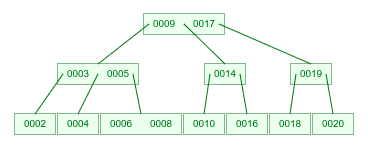
\includegraphics[]{b-trees/b-tree-example.png}

    \noindent Odmianą B-drzew są drzewa B+, które różnią się tym, że wszystkie wartości trzymane są w liściach oraz mają powiązania pomiędzy liśćmi (tak aby można było po kolei przejść wszystkie wartości w liściach).

    \subsection{Wyszukiwanie}
    Wyszukiwanie przebiega bardzo podobnie jak w drzewie BST, z tą różnicą, że nie mamy tylko lewego i prawego poddrzewa, a możemy mieć ich więcej, więc musimy zadecydować, do którego pójść.
    Oczywiście szukana wartość może również znajdować się na danym poziomie. Wtedy kończymy wyszukiwanie.
    Ponieważ rząd drzewa zazwyczaj jest wysoki (np. 1024), aby usprawnić wyszukiwanie zadanej wartości w danym węźle, najczęściej używamy wyszukiwania binarnego. \\

    \subsection{Wstawianie}
    Aby wstawić wartość wyszukujemy liść, do którego powinna trafić, a następnie wstawiamy ją w odpowiednie miejsce w tym liściu. \\
    \noindent Jeżeli jednak okazałoby się, że liść ma już za dużo kluczy (wartości) ($\geq K$), wtedy musimy go podzielić - jedną z wartości z liścia przenosimy w odpowiednie miejsce do rodzica, a jako prawego i lewego syna tej przeniesionej wartości wstawiamy odpowiednio liście powstałe po podzieleniu tego oryginalnego liścia. \\
    \noindent Jeżeli okazałoby się, że po przeniesieniu wartości z liścia do rodzica, rodzic ma za dużo kluczy (wartości), całą operację dzielenia powtarzamy rekurencyjnie na rodzicu - w razie potrzeby aż do korzenia. \\

    \subsection{Usuwanie}
    Usuwanie rozpoczynamy od znalezienia wartości, którą chcemy usunąć \\
    \noindent Następnie bierrzemy największą wartość z lewego podrzewa lub najmniejszą wartość z prawego poddrzewa i wstawiamy w miejsce usuwanego elementu \\
    \noindent Jeżeli w drzewie zostały naruszone warunki dotyczące ilości dozwolonych elementów w węźle, musimy to drzewo zrównoważyć. Proces ten jest generalnie dośc skomplikowany i ciężki do opisania algorytmem ze względu na mnogość możliwych przypadków, dlatego najlepiej spojrzeć na część praktyczną i przykłady.

    \newpage


    \section{Drzewa AVL: rotacje, operacje z wykorzystaniem rotacji i ich złożoność.}
    Drzewa AVL są odmianą drzew BST, w której dla każdego węzła mamy dodatkowy warunek: różnica między wysokością prawego i lewego poddrzewa danego węzła nie może byc większa niż 1.
    Spełnienie tego warunku zapewnia nam dobre zrównoważenie drzewa, a co za tym idzie utrzymanie szybkości operacji wywszukiwania w tym drzewie.\\

    \noindent Operacja wyszukiwania w drzewie AVL jest identyczna, jak dla zwykłego drzewa BST, natomiast w przypadku operacji wstawiania i usuwania, przebiegają one na początku tak samo jak w zwykłych BST, natomiast potem w razie potrzeby należy drzewo zrównoważyć poprzez rotacje. \\

    \noindent Operacje wyszukiwania, wstawiania oraz usuwania mają złożoność $O(\log_{2} n)$, gdzie n to ilość elementów w drzewie

    \subsection{Rotacje}
    \begin{multicols}{2}
        \textbf{Rotacja RR} \\

        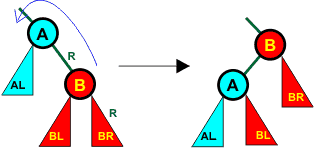
\includegraphics[width=0.8\linewidth]{avl-trees/rr-rotation.png}
        \columnbreak \\
        \textbf{Rotacja LL} \\

        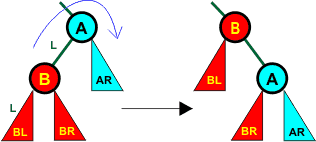
\includegraphics[width=0.8\linewidth]{avl-trees/ll-rotation.png}
    \end{multicols}

    \textbf{Rotacja RL} \\

    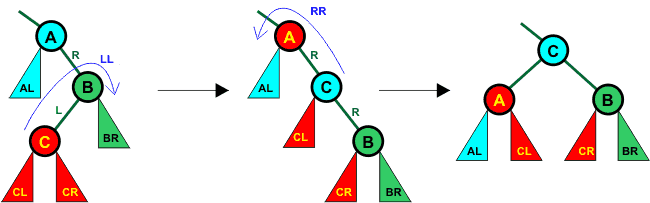
\includegraphics[width=\linewidth]{avl-trees/rl-rotation.png} \\

    \textbf{Rotacja LR} \\

    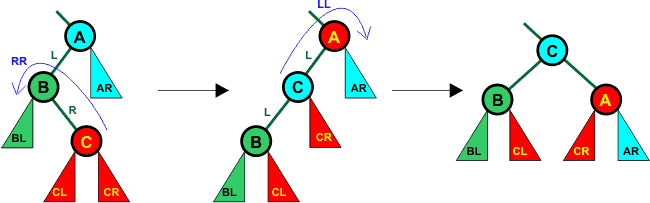
\includegraphics[width=\linewidth]{avl-trees/lr-rotation.png} \\

    \noindent Gdy \texttt{nierównowaga drzewa} idzie dwa razy na prawo (tzn. gdy dla danego węzła prawe poddrzewo jest głębsze niż lewe i potem dla pierwszego węzła prawego poddrzewa jego prawe poddrzewo jest głębsze) do zbalansowania używamy rotacji RR, natomiast, gdy nierównowaga idzie najpierw na prawo potem na lewo, używamy rotacji RL, itd.

    \newpage

    \section{Algorytmy przeszukiwania wszerz i w głąb w grafach.}

    Algorymy przeszukiwania grafu polegają na przejściu przez wszystkie osiągalne z wierzchołka
    startowego $s$ wierzchołki grafu $G$.

    \subsection{Przeszukiwanie grafu wszerz (\textit{breadth first search}, BFS)}

    \subsubsection{Algorytm}

    Do przeszukiwania użyjemy kolejki $Q = \{s\}$. Ponadto używamy koloru czarnego do
    oznaczania odwiedzonych już wierzchołków.\[\]
    Dopóki kolejka nie jest pusta:
    \begin{enumerate}
        \item Zdejm $x$ z kolejki
        \item Pomaluj $x$ na czarno
        \item Dla każdego niepomalowanego na czarno $v$, sąsiadującego z $x$ wrzuć
        $v$ do kolejki
    \end{enumerate}

    \subsubsection{Cechy}

    \begin{enumerate}
        \item Zlożoność obliczeniowa: $\theta(e + v)$
        \item Złożoność pamięciowa: $\theta(v)$
        \item Kompletność: BFS dla nieskończonego grafu zwróci wszystkie poprawne
        odpowiedzi, w przeciwieństwie do DFS.
    \end{enumerate}

    \subsubsection{Wariacje algorytmu}

    \begin{itemize}
        \item Faktyczne "przeszukiwanie": zwracamy wieszchołek, jeśli jego wartość jest
        równa poszukiwanej.
        \item Przypisywanie wierzchołkom odległości od $s$.
        \item Przypisanie wierzchołkom rodzica, w celu znalezienia drogi do $s$
    \end{itemize}

    \subsubsection{Zastosowania}

    \begin{itemize}
        \item Garbage collection
        \item Najkrótsza droga do $s$ (licząć liczbę krawędzi)
        \item Wykrywanie cykli grafu nieskierowanego
        \item Sprawdzanie dwudzielności grafu
        \item Social networking
        \item Algorytmy sieci przepływowych (np. wyznaczanie maksymalnego przepływu)
        \item Crawlery
    \end{itemize}

    \subsection{Przeszukiwanie grafu wgłąb (\textit{depth first search}, DFS)}

    \subsubsection{Algorytm}

    Używamy koloru czarnego do oznaczania odwiedzonych już wierzchołków.\[\]
    Dla danego wierzchołka $x$ (zaczynając od $s$):
    \begin{enumerate}
        \item Pomaluj $x$ na czarno
        \item Wywołaj się rekurencyjnie dla każdego niepomalowanego na czarno $v$,
        sąsiadującego z $x$
    \end{enumerate}


    \subsubsection{Wersja z zapamiętywaniem rodzica}

    Słownik $P = \{s : null\}$ przypisuje każdemu wierzchołkowi (poza $s$) rodzica. Używamy
    koloru czarnego do oznaczania odwiedzonych już wierzchołków, oraz szarego do
    wierzchołków właśnie odwiedzanych.\[\]
    Dla danego wierzchołka $x$ (zaczynając od $s$):
    \begin{enumerate}
        \item Pomaluj $x$ na szaro
        \item Dla każdego białego $v$, sąsiadującego z $x$:
        \begin{enumerate}
            \item $P[v] = x$
            \item Wywołaj się rekurencyjnie na $v$
        \end{enumerate}
        \item Pomaluj $x$ na czarno
    \end{enumerate}

    \subsubsection{Cechy}

    \begin{enumerate}
        \item Zlożoność obliczeniowa: $\theta(e + v)$
        \item Złożoność pamięciowa: $\theta(v)$
        \item Niekompletność dla grafów nieskończonych
    \end{enumerate}

    \subsubsection{Wariacje algorytmu}

    \begin{itemize}
        \item Faktyczne "przeszukiwanie": zwracamy wieszchołek, jeśli jego wartość jest
        równa poszukiwanej.
        \item Przypisywanie wierzchołkom odległości od $s$.
        \item Przypisanie wierzchołkom rodzica, w celu znalezienia drogi do $s$
    \end{itemize}

    \subsubsection{Zastosowania}

    \begin{itemize}
        \item Garbage collection
        \item Minimalne drzewo rozpinające (dla grafów nieważonych)
        \item Wykrywanie cykli w grafie skierowanym
        \item Sortowanie topologiczne
        \item Wykrywanie cykli grafu nieskierowanego
        \item Algorytmy sieci przepływowych (np. wyznaczanie maksymalnego przepływu)
        \item Crawlery
        \item Labirynty
    \end{itemize}

    \newpage

    \section{Algorytmy wyszukiwania najkrótszej ścieżki (Dijkstry oraz Bellmana-Forda).}

    W algorytmach wyszukiwania najkrótszej ścieżki używamy procedury \textit{relax(u, v, w)},
    sprawdzającej, czy ścieżka z $u$ do $w$ przez $v$ jest krótsza od aktualnie najkrótszej
    ścieżki.
    \\~\\
    \textit{relax(u, v, w)}:
    \vskip 0pt Jeśli $D[u, w] = D[u, v] + D[v, w]$ to:\\
    \hspace*{1cm} $D[u, w] = D[u, v] + D[v, w]$\\
    \hspace*{1cm} $P[u, w] = v$\\

    \subsection{Algorytm Dijkstry}

    Algorytm Dijkstry pozwala na wyliczenie w grafie $G = \{V, E\}$ najkrótszej ścieżki od wierzchołka
    startowego $s$ do wszystkich pozostałych wierzchołków. $|V| = v, |E| = e$

    \subsubsection{Algorytm}

    Posługujemy się słownikiem $P = \{\}$ przypisującym każdemu wierzchołkowi
    rodzica (w celu znalezienia ścieżki), słownikiem $D$ oznaczającym odległość
    wierzchołków od $s$ oraz kolejką priorytetową $S = \{v \in V : D[v]\}$ nieodwiedzonych
    wierzchołków. $D[s] = 0; D[\forall v \in V \setminus \{s\}] = \infty$.
    \[\]
    Używamy uproszczonej procedury \textit{relax} - wierzchołkiem startowym ($u$) jest zawsze $s$
    \[\]
    \textit{relax(v, w)}:
    \vskip 0pt Jeśli $D[w] = D[v] + e_{v \rightarrow w}$ to:\\
    \hspace*{1cm} $D[w] = D[v] + e_{v \rightarrow w}$ \\
    \hspace*{1cm} $P[w] = v$ \\

    \[\]
    Dopóki $S \neq \o$:
    \begin{enumerate}
        \item Usuń wierzchołek $v$ o najmniejszej wartości z $S$
        \item Dla każdego wierzchołka $w$ sąsiadującego z $v$ wywołaj \textit{relax(v, w)}
    \end{enumerate}

    \subsubsection{Złożoność}

    \begin{itemize}
        \item Inicjalizacja - $\theta(v)$
        \item $\theta(v)$ usunięć z kolejki
        \item $O(e)$ pomniejszeń wartości w $D$
        \item Przy pomocy kopca binarnego możemy uzyskać $O(log(v))$ dla pomniejszenia
        wartości, $O(log(v))$ dla usunięcia z kolejki. Złożoność:
        $\theta((e + v)log(v))$

        \item Przy pomocy kopca Fibonacciego możemy uzyskać $\theta(1)$ dla pomniejszenia
        wartości, $\theta(log (v))$ dla usunięcia z kolki. Złożoność:
        $O(v \cdot log(v) + e)$
    \end{itemize}

    \subsubsection{Cechy}

    \begin{itemize}
        \item Nie działa poprawnie dla grafów z wagami ujemnymi
        \item Algorytm zachłanny
    \end{itemize}

    \subsection{Algorytm Bellmana-Forda}

    Algorytm Bellmana-Forda pozwala na wyliczenie w grafie $G$ najkrótszej ścieżki z
    wierzchołka startowego $s$ do wszystkich pozostałych wierzchołków.

    \subsubsection{Algorytm}

    Posługujemy się słownikiem $P = \{\}$, przypisującym każdemu wierzchołkowi
    rodzica (w celu znalezienia ścieżki), słownikiem $D$ oznaczającym odległość
    wierzchołków\\ od $s$. $D[s] = 0; D[v] = \infty \; \forall v \in V \setminus \{s\}$.
    \[\]
    Ponownie używamy uproszczonej procedury \textit{relax}.

    \[\]
    Dla każdego wierzchołka w $V \setminus \{s\}$:
    \vskip 0pt Wywołaj \textit{relax(u, v)} dla każdej krawędzi $(u, v) \in E$
    \[\]

    Dodatkowo można wykonać sprawdzenie, czy w grafie nie ma cykli o wadze ujemnej:

    \[\]
    Dla każdej krawędzi $(u, v) \in E$:
    \vskip 0pt Jeśli $D[v] > D[u] + e_{u \rightarrow v}$, to
    istnieje cykl o wadze ujemnej.
    \subsubsection{Złożoność}

    $O(v \cdot e)$

    \subsubsection{Cechy}

    \begin{itemize}
        \item Działa poprawnie dla grafów z wagami ujemnymi (bez cykli o wagach ujemnych)
        \item Pozwala decydować, czy graf ma cykle ujemne
        \item Używany w protokole RIP
        \item Algorytm można zoptymalizować: jeśli w danej iteracji nie dokonał zmiany,
        należy przerwać jego działanie (ścieżki już są najkrótsze)
    \end{itemize}

    \subsection{Algorytm Floyda-Warshalla}

    Algorytm Floyda-Warshalla pozwala wyliczyć najkrósze ścieżki pomiędzy wszystkimi
    wierzchołkami w grafie $G$ (nieposiadającym ujemnych cykli).

    \subsubsection{Algorytm}

    Posługujemy się słownikiem $P = \{\}$, przypisującym parze $(u, w)$ rodzica dla $u$,
    na ścieżce od $u$ do $w$, słownikiem $D$ przypisującym parze $(u, w)$ długość
    najkrószej (aktualnie) ścieżki od $u$ do $w$.\\
    $D[(u, w) : u, w \in V] =
    \begin{cases}
        0, &\text{ jeśli } u = w\\
        e_{u \rightarrow w}, &\text{ jeśli } (u, w) \in E\\
        \infty, &\text{ jeśli } (u, w) \notin E
    \end{cases}$.
    \[\]

    Wywołaj  \textit{relax(u, v, w)} dla każdej trójki $(u, v, w) : u, w, v \in V$ wywołaj
    \subsubsection{Złożoność}
    $\theta(v^3)$

    \subsubsection{Cechy}
    \begin{itemize}
        \item Prostota
        \item Pozwala obliczyć za jednym razem wszystkie ścieżki pomiędzy wierzchołkami
        \item Działa dla grafów z krawędziami ujemnymi (ale nie z cyklami ujemnymi)
        \item Złożoność jest niezależna od gęstości grafu
    \end{itemize}

    \section{Programowanie dynamiczne: podział na podproblemy, porównanie z metodą "dziel i zwyciężaj".}

    \begin{definition}
        \textbf{Programowanie dynamiczne}

        Technika projektowania algorytmów polegająca na \textbf{podziale problemu na mniejsze podproblemy} względem kilku parametrów (podobnie jak w metodzie dziel i zwyciężaj).

        Wyniki rozwiązywania podproblemów są  \textbf{zapisywane w tabeli}, dzięki czemu w przypadku natrafienia na ten sam podproblem nie trzeba go ponownie rozwiązywać.

        Cechy
        \begin{itemize}
            \item Problem posiada powtarzające się podproblemy
            \item Podproblemy musi cechować \textbf{własność optymalnej podstruktury}
            \item Zastosowanie brute force prowadzi do \textbf{ponadwielomianowej} liczby rozwiązań podproblemów, podczas gdy sama liczba różnych podproblemów jest wielomianowa
        \end{itemize}

        Niejednokrotnie stosowanie techniki programowania dynamicznego daje w rezultacie algorytm pseudowielomianowy.
    \end{definition}

    \begin{definition}
        \textbf{Własność optymalnej podstruktury}

        Oznacza, że optymalne rozwiązanie problemu jest \textbf{funkcją optymalnych rozwiązań podproblemów}, czyli znając optymalne rozwiązania podproblemów można efektywnie wyznaczyć rozwiązanie problemu.
    \end{definition}

    \begin{definition}
        \textbf{Funkcja celowa}

        W zadaniach programowania liniowego liniowa funkcja, dla której szukane jest optymalne rozwiązanie minimum lub maksimum. Dla zdefiniowanego zadania programowania liniowego

        Optymalizacja – problem polegający na znalezieniu ekstremum zadanej funkcji celu.
    \end{definition}

    Metody Programowania Dynamicznego
    \begin{itemize}
        \item Metoda zstępująca z zapamiętywaniem polega na rekurencyjnym wywoływaniu funkcji z zapamiętywaniem wyników. Metoda ta jest podobna do metody dziel i zwyciężaj – różni się od niej tym, że jeśli rozwiązanie danego problemu jest już w tabeli z wynikami, to należy je po prostu stamtąd odczytać.
        \item Metoda wstępująca polega na rozwiązywaniu wszystkich możliwych podproblemów, zaczynając od tych o najmniejszym rozmiarze. Wówczas w momencie rozwiązywania podproblemu na pewno są już dostępne rozwiązania jego podproblemów. W tym podejściu nie zużywa się pamięci na rekurencyjne wywołania funkcji. Może się jednak okazać, że część podproblemów została rozwiązana nadmiarowo (nie były one potrzebne do rozwiązania głównego problemu).
    \end{itemize}

    Klucz do zaprojektowania algorytmu tą techniką leży w znalezieniu \textbf{równania rekurencyjnego} opisującego optymalną wartość \textbf{funkcji celu} dla danego problemu jako funkcji optymalnych wartości funkcji celu dla podproblemów o mniejszych rozmiarach. Programowanie dynamiczne znajduje optymalną wartość funkcji celu dla całego zagadnienia, rozwiązując podproblemy od najmniejszego do największego i zapisując optymalne wartości w tablicy. Pozwala to zastąpić wywołania rekurencyjne odwołaniami do odpowiednich komórek wspomnianej tablicy i gwarantuje, że każdy podproblem jest rozwiązywany tylko raz. Rozwiązanie ostatniego z rozpatrywanych podproblemów jest na ogół wartością rozwiązania zadanego zagadnienia.

    Przykład - Ciąg Fibonacci'ego

    \begin{verbatim}
        # Programowanie dynamiczne wstępujące, wersja z listą.
        def fibonacci(n):
        F = [0] + n * [1]   # trzymamy wszystkie wartości
        for i in range(2, n+1):
        F[i] = F[i-1] + F[i-2]
        return F[n]
    \end{verbatim}

    \begin{verbatim}
        # Programowanie dynamiczne zstępujące.
        FIBONACCI = {0:0, 1:1}   # globalny słownik

        def fibonacci(n):
        global FIBONACCI
        if n not in FIBONACCI:
        FIBONACCI[n] = fibonacci(n-1) + fibonacci(n-2)
        return FIBONACCI[n]
    \end{verbatim}

    \newpage

    \section{Algorytm zachłanny: przykład optymalnego i nieoptymalnego wykorzystania.}

    \begin{definition}
        Algorytmy zachłanne (ang. greedy algorithms)

        Algorytmy podejmujące w każdym kroku taką decyzję, która w danej chwili jest najkorzystniejsza (\textbf{lokalnie optymalna}) licząc, że doprowadzi to do znalezienia rozwiązania \textbf{globalnie optymalnego}.

        Cechy

        \begin{itemize}
            \item Nie zawsze znajdują rozwiązanie optymalne
            \item Są podzbiorem algorytmów \textbf{heurystycznych}
            \item Są to algorytmy \textbf{deterministyczne} – nie ma w nich losowości
        \end{itemize}

    \end{definition}
    
    % Tu był przykład z wydawaniem reszty. Usuwam, bo ciężko zdefiniować "nieoptymalne" rozwiązanie - ktoś na egzaminie mógłby mieć przez to problem.

    Przykład - Pakowanie plecaka

    \begin{verbatim}
        posortuj nierosnąco przedmioty według wartości c[j]/w[j]
        aktualna_waga:=0

        for i:=1 to n do
        if w[i] + aktualna_waga <= W then
        dodaj i-ty przedmiot do plecaka
        aktualna_waga := aktualna_waga + w[i]
    \end{verbatim}

    Dane wejściowe, dla których algorytm będzie działał
    \begin{itemize}
        \item Optymalnie

        Pjemność plecaka: 8

        Dane wejściowe: 5, 3, 2, 1, 1, 1, 1, 1, 1, 1, 1

        Rozwiązanie: 5 + 3 + 2

        \item Nieoptymalnie

        Pojemność plecaka: 7

        Dane wejściowe: 3, 3, 2, 2

        Rozwiązanie: 3 + 3 = 6 :(

        Rozwiązanie optymalne: 3 + 2 + 2 = 7

    \end{itemize}

    \newpage

    \section{Kolorowania wierzchołkowe (grafów planarnych) i krawędziowe grafów, algorytmy i ich złożoności.}

    \subsection{Kolorowanie krawędziowe grafów}
    Problem kolorowania krawędzi, podobnie jak klasycznego kolorowania wierzchołków, jest NP-trudny – nie istnieją wielomianowe algorytmy kolorujące grafy zawsze w sposób optymalny.
    \\\\
    Przykład nieopytymalnego algorytmu kolorowania krawędziowego:
    \begin{enumerate}
        \item Użyj BFS (Breadth First Search - Przeszukiwanie wszerz) do poruszania się po grafie.
        \item Wybierz wierzchołek i nadaj różne kolory jego krawędziom.
        \item Przejdź do kolejnego wierzchołka.
        \item Powtarzaj aż wszyskie krawędzie zostaną pokolorowane.
    \end{enumerate}

    \subsection{Kolorowanie wierzchołkowe grafów planarnych}

    \begin{definition}
        Graf planarny - graf, który można narysować na płaszczyźnie tak, by krzywe obrazujące krawędzie grafu nie przecinały się ze sobą.
    \end{definition}

    \begin{theorem}
        Liczba chromatyczna grafu planarnego jest równa lub mniejsza niż 4
    \end{theorem}

    Każdy graf planarny można pokolorować 5 kolorami w czasie liniowym.





    \newpage

    \section{Algorytmy wyszukiwania minimalnego drzewa rozpinającego: Boruvki, Prima i Kruskala.}

    \subsection{Algorytm Boruvki}
    \begin{enumerate}
        \item Weź wszystkie wierzchołki, ale bez krawędzi - każdy wierzchołek jest osobnym drzewem.
        \item Dla każdego drzewa znajdź krawędź o najmniejszej wadze w oryignalnym grafie, która łączy je z innym drzewem.
        \item Dodaj tę krawędź do MST.
        \item Powtarzaj, dopóki drzewa nie połączyły się w jedno.
    \end{enumerate}
    \textbf{Złożoność:} $O(ElogV)$.


    \subsection{Algorytm Prima}
    \begin{enumerate}
        \item Zainicjalizuj MST jednym wierzchołkiem, wybranym losowo z grafu.
        \item Spośród krawędzi łączących MST z wierzchołkami jeszcze w nim niebędącymi wybierz tę, która ma najmniejszą wagę, i dodaj ją do MST.
        \item Powtarzaj krok 2 aż wszystkie wierzchołki znajdą się w MST.
    \end{enumerate}
    \textbf{Złożoność:} Zależy od użytych struktur danych. $O(V^2)$ lub $O(ElogV)$, jeśli użyta została lista sąsiedztwa.



    \subsection{Algorytm Kruskala}

    \begin{enumerate}
        \item Posortuj krawędzie niemalejąco pod względem wag.
        \item Wybierz krawędź o najmniejszej wadze. Sprawdź czy tworzy cykl z MST utworzonym do tej pory. Jeśli nie, uwzględnij tą krawędź w MST. W przeciwnym wypadku, odrzuć.
        \item Powtarzaj krok 2 aż otrzymasz $V-1$ krawędzi w MST
    \end{enumerate}

    \textbf{Złożoność:} Sortowanie krawędzi zajmuje $O(ElogE)$. Po sortowaniu, iterujemy po krawędziach i używamy algorytmu find-union który może zająć $O(logV)$. Zatem ogólna złozoność to $O(ElogE+ElogV)$. Wartość E jest mniejsza niż $V^2$, więc $O(logV)$ $=$ $O(logE)$. Złożoność: $O(ElogE)$ lub $O(ElogV)$.

    \newpage

    \section{Najważniejsze algorytmy wyznaczania otoczki wypukłej zbioru punktów w układzie współrzędnych (Grahama, Jarvisa, algorytm przyrostowy (quickhull)).}

    \begin{definition}
        \textbf{Algorytm Grahama} - złożoność $O(n \log n)$.
        \begin{enumerate}
            \item Wybierz punkt (ozn. O) o najmniejszym y (jeśli jest kilka ex aequo, to ten z nich o najmniejszym x).
            \item Posortuj pozostałe punkty leksykograficznie względem:
            \begin{itemize}
                \item kąta pomiędzy wektorem $OP_i$ a osią X,
                \item długości wektora $OP_i$.
            \end{itemize}
            \item Przeglądaj listę posortowanych punktów:
            \begin{itemize}
                \item Od bieżącej pozycji weź trzy kolejne punkty (ozn. A, B, C).
                \item Jeśli punkt B leży na zewnątrz trójkąta AOC, to może należeć do otoczki wypukłej. Przejdź do następnej trójki punktów.
                \item Jeśli punkt B leży wewnątrz trójkąta AOC, to znaczy, że nie należy do otoczki. Usuń punkt B z listy i cofnij się o jedną pozycję (o ile bieżąca pozycja jest różna od początkowej).
            \end{itemize}
            \item Pozostałe na liście punkty stanowią otoczkę wypukłą.
        \end{enumerate}
    \end{definition}

    \begin{definition}
        \textbf{Algorytm Jarvisa} - średnia złożoność $O(kn)$, gdzie n - liczba punktów, k - liczba punktów należących do otoczki; pesymistyczna - $O(n^2)$.
        \begin{enumerate}
            \item $P_1$ – punkt na otoczce wypukłej o najmniejszej współrzędnej y (jeśli jest więcej niż jeden, wybierany jest ten o najmniejszej współrzędnej x),
            \item $P_{0}:=[-\infty ,y(P_{1})]$,
            \item $i:=1$,
            \item powtarzaj:
            \begin{itemize}
                \item $P_{i+1}$ – punkt $N$, dla którego kąt $P_{i-1}P_{i}N$ jest największy,
                \item jeśli $N=P_{1}$, koniec iterowania,
                \item $i:=i+1$,
            \end{itemize}
            \item ostatecznie otoczkę tworzą punkty $P_{1\dots i}$.
        \end{enumerate}

        Implementację można usprawnić, odrzucając w każdej iteracji punkty znajdujące się po prawej stronie wektora $P_{1}P_{i}$, ponieważ na pewno nie będą należały do otoczki. Zabieg ten nie wpływa jednak na asymptotyczną złożoność obliczeniową algorytmu.
    \end{definition}

    \begin{definition}
        \textbf{Quickhull} - średnia złożoność $O(n \log n)$, pesymistyczna złożoność - $O(n^2)$.

        QuickHull(P):
        \begin{enumerate}
            \item Znajdź w $P$ punkty o minimalnym i maksymalnym x (A oraz B).
            \item Podziel $P$ na dwa podzbiory $S_1$ i $S_2$ znajdujące się nad i pod prostą $AB$.
            \item Wywołaj rekurencyjnie QuickHull(A, B, $S_1$) i QuickHull(B, A, $S_2$).
        \end{enumerate}

        QuickHull(A, B, P) - funkcja pomocnicza:
        \begin{enumerate}
            \item Jeśli $P$ jest pusty – koniec.
            \item Jeśli $P$ ma jeden element, ten punkt należy do otoczki – koniec.
            \item W przeciwnym razie:
            \begin{itemize}
                \item Znajdź w $P$ punkt $C$ najbardziej oddalony od prostej $AB$. Ten punkt należy do otoczki wypukłej.
                \item Odrzuć wszystkie punkty z wnętrza trójkąta $ABC$, nie mogą należeć do otoczki.
                \item Znajdź zbiór $S_1$ punktów znajdujących się po prawej stronie prostej $AC$C oraz analogiczny
                zbiór $S_2$ dla prostej $BC$. (Stronę określa znak równania ogólnego prostej).
                \item Wywołaj rekurencyjnie QuickHull(A, C, $S_1$) i QuickHull(B, C, $S_2$).
            \end{itemize}
        \end{enumerate}
    \end{definition}

    \newpage

    \section{Problemy P, NP, NP-zupełne i zależności między nimi. Hipoteza P vs. NP.}
    \begin{definition}
        \textbf{Problem P} (ang. \textit{deterministic polynomial}, deterministycznie wielomianowy) – problem decyzyjny,
        dla którego rozwiązanie można \textbf{znaleźć} w czasie wielomianowym.
    \end{definition}

    \begin{definition}
        \textbf{Problem NP} (ang. \textit{nondeterministic polynomial}, niedeterministycznie wielomianowy) – problem
        decyzyjny, dla którego rozwiązanie można \textbf{zweryfikować} w czasie wielomianowym.
    \end{definition}

    \begin{theorem}
        $\mathbf{P \stackrel{?}{=} NP}$. Każdy problem P jest NP, jednak nie wiadomo czy istnieje problem NP niebędący P.
    \end{theorem}

    \begin{definition}
        \textbf{Problem NP-zupełny} (ang. \textit{NP-Complete}) – taki problem \textbf{NP}, do którego można \textbf{w czasie wielomianowym zredukować} dowolny inny problem NP. Czasami zamiast redukcji w czasie wielomianowym używa się redukcji w pamięci logarytmicznej.
    \end{definition} 
    Stąd wynika, że jeśli potrafimy rozwiązać jakikolwiek problem NP-zupełny w czasie wielomianowym,
    to potrafimy rozwiązać w takim czasie wszystkie problemy NP.

    \newpage

    \section{Automat minimalny, wybrany algorytm minimalizacji.}
    \subsection{Automat minimalny}
    \begin{definition}
        Automat $\mathcal{A} = (S, A, f, s_{0}, T)$ rozpoznający język L jest minimalny, jeśli posiada najmniejszą liczbę stanów spośród wszystkich automatów rozpoznających język L.
    \end{definition}

    \begin{definition}
        Dla dowolnego języka $L \in \mathcal{REC}(A^{*})$ automat
        \begin{center}
            $\mathcal{A}_{P_{L}^{r}} = (A^{*} / P_{L}^{r}, A, f^{*}, [1]_{P_{L}^{r}}, T)$,
        \end{center}
        gdzie $T = \{[w]_{P_{L}^{r}} : w \in L \}$ jest automatem minimalnym rozpoznającym język L
    \end{definition}
    \begin{definition}
        \textbf{Konstrukcja automatu minimalnego z wykorzystaniem prawej kongruencji automatowej} \\
        $L \subset A^{*}$ - dowolny język \\
        $\Theta_{L} \subset A^* \times A^*$ - relacja równoważności dzieląca $A^*$ na dwie klasy:
        \begin{center}
            L oraz $A^* \setminus L$
        \end{center}
        $\rho_i$ dla $i \in \mathbb{N}$ - zstępujący ciąg relacji: \\
        $\rho_1 = \Theta_L$, \\
        $\rho_i = \{(u, w) \in A^* \times A^* : \forall a \in A \cup \{\textbf{1}\}: (ua, wa) \in \rho_{i-1} \}$ dla i = 2, ... \\
        Wtedy
        \begin{center}
            $\bigcap\limits_{i \in \mathbb{N}} \rho_i = P^r_L$
        \end{center}
    \end{definition}


    \subsection{Minimalizacja automatu}
    \begin{definition}
        \textbf{Algorytm ``Minimalizuj 1''} \\
        \url{http://wazniak.mimuw.edu.pl/index.php?title=J\%C4\%99zyki\%2C_automaty_i_obliczenia/Wyk\%C5\%82ad_5:_Algorytmy_konstrukcji_automatu_minimalnego} \\
        Wejście L - język \\
        Wyjście: automat minimalny $\mathcal{A} = (S_L, A, f_F, s_L, T_L)$ taki, że $L\mathcal{A} = L$
        \begin{lstlisting}
            $S_L \leftarrow \{L\};$
            Put$(\mathcal{L}, L);$
            while $\mathcal{L} \neq \emptyset$ do
            M $\leftarrow$ \textbf{zdejmij} $(\mathcal{L})$;
            foreach $a \in A$ do
            N $\leftarrow a^{-1}M$;
            if $N \cap S_L = \emptyset$ then
            $S_L \leftarrow S_L \cup \{N\}$;
            Put$(\mathcal{L}, N);$
            end if
            end for
            end while
            foreach $M \in S_L$ do
            foreach $a \in A$ do
            $f_L(M, a) \leftarrow a^{-1}M$;
            end for
            end for
            $s_L \leftarrow L$;
            $T_L \leftarrow \{u^{-1}L : u \in L\}$;
            return $\mathcal{A}'$;
        \end{lstlisting}
    \end{definition}

    \section{Lemat o pompowaniu dla języków regularnych.}
    \begin{definition}
        Niech $L \subset A^*$ będzie językiem rozpoznawalnym. Istnieje liczba naturalna $N \geq 1$ taka, że dowolne słowo $w \in L$ o długości $|w| \geq N$ można rozłożyć na katenację:
        \begin{center}
            $w = v_1uv_2$
        \end{center}
        gdzie $v_1, v_2 \in A^*, u \in A^+, |v_1u| < N$ oraz
        \begin{center}
            $v_1u^*v_2 \subset L$
        \end{center}
    \end{definition}

    \begin{definition}
        Jeśli rozpoznawalny język $L \subset A^*$ jest nieskończony, to istnieją
        $v_1, v_2 \in A^*, u \in A^+$, takie, że
        \begin{center}
            $v_1u*v_2 \subset L$
        \end{center}
    \end{definition}

    \newpage

    \section{Warunki równoważne definicji języka regularnego: automat, prawa kongruencja syntaktyczna, wyrażenia regularne.}
    \subsection{Wyrażenia regularne}

    \begin{definition}
        \textbf{Rodzina regularnych podzbiorów}

        Niech $A$ będzie dowolnym zbiorem. Rodzina $REG(A^*)$ regularnych podzbiorów
        $A^*$ to najmniejsza rodzina $R$ podzbiorów $A^*$ taka, że:

        \begin{enumerate}
            \item $\emptyset \in R, \forall a \in A$ ${a} \in R$
            \item jeśli $X, Y \in R$, to: $X \cup Y, X \cdot Y \in R$
            \item jeśli $X \in R$, to: $X^* = \bigcup\limits_{n = 0}^{\infty} X^n \in R$
        \end{enumerate}
    \end{definition}

    \begin{definition}
        \textbf{Wyrażenie regularne}

        Niech $A$ będzie dowolnym alfabetem, a zbiór $\{+, \star, \emptyset, (,)\}$
        alfabetem takim, że $A \cap \{+, \star, \emptyset, (,)\} = \emptyset$.

        Słowo $\alpha \in (A \cup \{+, \star, \emptyset, (,)\})^*$ jest wyrażeniem regularnym
        nad alfabetem A wtedy i tylko wtedy, gdy:

        \begin{enumerate}
            \item $\alpha = \emptyset$
            \item $\alpha = a \in A$
            \item $\alpha$ jest w postaci $(\beta + \gamma), (\beta\gamma), \gamma^*$, gdzie
            $\beta, \gamma$ są wyrażeniami regularnymi nad alfabetem A
        \end{enumerate}
    \end{definition}

    Rodzinę wyrażeń regularnych nad $A$ nazywamy $WR$.

    \subsection{Automat skończony}

    \begin{definition}
        \textbf{Automat}

        Automatem nad alfabetem A nazywamy system $\mathcal{A} = (S, f)$ w którym:
        \begin{itemize}
            \item S jest dowolnym zbiorem, zwanym zbiorem stanów
            \item $f : S \times A \rightarrow S$ jest funkcją przejść
        \end{itemize}

        Automat $\mathcal{A}$ nazywamy skończonym, jeśli zbiór S jest skończony

        Automat $\mathcal{A}$ ze stanem $s \in S$ taki, że
        $$f(a, A^*) = Ss$$
        nazywamy automatem z generatorem s.
    \end{definition}

    \begin{definition}
        \textbf{Język rozpoznawalny}

        Język $L \subset A^*$ jest rozpoznawalny wtedy i tylko wtedy, gdy istnieją:
        \begin{itemize}
            \item Automat skończony $\mathcal{A} = (S, f)$
            \item stan $s_0 \in S$
            \item zbiór $T \subset S$
        \end{itemize}

        takie, że
        $$ L = \{w \in A^* : f(s_0, w) \in T\}$$
        $s_0$ - stan początkowy \\
        T - zbiór stanów końcowych automatu
        $$\mathcal{A} = (S, A, f, s_0, T)$$
        $L = L(\mathcal{A})$ - język rozpoznawany przez automat $\mathcal{A}$\\
        $REC(A^*)$ - rodzina wszystkich języków rozpoznawalnych nad alfabetem A
    \end{definition}

    \subsection{Prawa kongruencja syntaktyczna}

    \begin{definition}
        \textbf{Prawa kongruencja}

        Każdy automat $\mathcal{A} = (S, f)$ z generatorem $s_0$ wyznacza na wolnym
        monoidzie $A^*$ prawą kongruencję $\sim_\mathcal{A}$:
        \[\]
        $\forall u, v \in A^*$
        $$u \sim_\mathcal{A} v \Leftrightarrow f(s_0, u) = f(s_0, v)$$

        Relacja $\sim_{\mathcal{A}}$ ma skończony indeks wtedy i tylko wtedy, gdy automat
        $\mathcal{A}$ jest skończony.
    \end{definition}

    \begin{theorem}
        Każda prawa kongruencja $p \subset (A^*)^2$ wyznacza automat, zwany ilorazowym
        $$\mathcal{A}_p = (A^* /_{p}, f^*), \; \mathrm{gdzie} \; f^*([w]_p, u) = [wu]_p$$
        \begin{itemize}
            \item $\mathcal{A}_p$ jest automatem z generatorem [1]$_p$

            \item $\mathcal{A}_p$ jest automatem skończonym wtedy i tylko gdy relacja $p$ ma skończony indeks
        \end{itemize}
    \end{theorem}

    \subsection{Warunki równoważne definicji języka regularnego}
    \begin{theorem}
        \textbf{Twierdzenie Kleenego}

        Dla każdego skończonego alfabetu A
        $$REC(A^*) = REG(^*)$$
    \end{theorem}

    \begin{theorem}
        Dla dowolnego języka regularnego $L \in A^*$ następujące warunki są równoważne:
        \begin{itemize}
            \item L = L(G) dla gramatyki G typu 3 (regularnej, lewoliniowej)
            \item L = L(G) dla gramatyki G prawoliniowej
            \item L = L($\mathcal{A}$) dla automatu deterministycznego $\mathcal{A}$
            \item L = L($\mathcal{A}_{ND}$) dla automatu niedeterministycznego $\mathcal{A}_{ND}$
            \item L = L($\mathcal{A}_{ND}$) dla automatu niedeterministycznego $\mathcal{A}_{ND}^p$ z pustymi przejściami

            \item L = $\|\alpha\|$ dla wyrażenia regularnego $\alpha$ nad alfabetem A
            \item L $\in REG(A^*)$
            \item monoid syntaktyczna M(L) jest skończony
            \item liczba różnych pochodnych Brzozowskiego dla języka
            L jest skończona
            \item L jest sumą wybranych klas równoważności pewnej prawej kongruencji na $A^*$
            o skończonym indeksie oraz L = $\bigcup\limits_{w \in L}[w]_p$
            \item istnieje skończony monoid M i homomorfizm
            $$\varphi : A^* \rightarrow M : L = \varphi^{-1}(\phi(L))$$
        \end{itemize}
    \end{theorem}

    \newpage
    \subsection{Konstrukcja automatu skończenie stanowego rozpoznającego wyrażenie regularne.}
    \begin{itemize}
        \item automat rozpoznający język pusty
        \begin{center}
            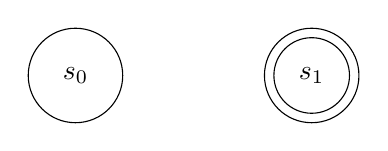
\begin{tikzpicture}[scale=0.2]
                \tikzstyle{every node}+=[inner sep=0pt]
                \draw [black] (13,-27) circle (3);
                \draw (13,-27) node {$s_0$};
                \draw [black] (28,-27) circle (3);
                \draw (28,-27) node {$s_1$};
                \draw [black] (28,-27) circle (2.4);
            \end{tikzpicture}
        \end{center}


        \item automat rozpoznający język $\{1\}$
        \begin{center}
            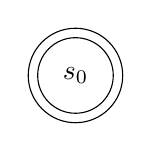
\begin{tikzpicture}[scale=0.2]
                \tikzstyle{every node}+=[inner sep=0pt]
                \draw [black] (29.4,-17.1) circle (3);
                \draw (29.4,-17.1) node {$s_0$};
                \draw [black] (29.4,-17.1) circle (2.4);
            \end{tikzpicture}
        \end{center}

        \item automat rozpoznający język $\{a\} \; \forall a \in A$
        \begin{center}
            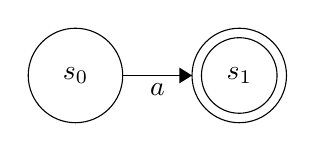
\begin{tikzpicture}[scale=0.2]
                \tikzstyle{every node}+=[inner sep=0pt]
                \draw [black] (29.4,-17.1) circle (3);
                \draw (29.4,-17.1) node {$s_0$};
                \draw [black] (39.8,-17.1) circle (3);
                \draw (39.8,-17.1) node {$s_1$};
                \draw [black] (39.8,-17.1) circle (2.4);
                \draw [black] (32.4,-17.1) -- (36.8,-17.1);
                \fill [black] (36.8,-17.1) -- (36,-16.6) -- (36,-17.6);
                \draw (34.6,-17.6) node [below] {$a$};
            \end{tikzpicture}
        \end{center}

        \newpage
        \item dla automatu $\mathcal{A}_r$ rozpoznającego wyrażenie $r$ i automatu $\mathcal{A}_r$ rozpoznającego wyrażenie $s$:
        $L(\mathcal{A}_x) = L(r + s)$ \\
        \noindent $\mathcal{A}_r = (S_r, A, f_r, s_{0r}, T_r) $ \\
        \noindent $\mathcal{A}_s = (S_s, A, f_s, s_{0s}, T_s) $ \\
        \noindent $\mathcal{A}_x = (S_x, A, f_x, s_{0x}, T_x) $ \\

        $$\mathcal{A}_s:$$
        \begin{center}
            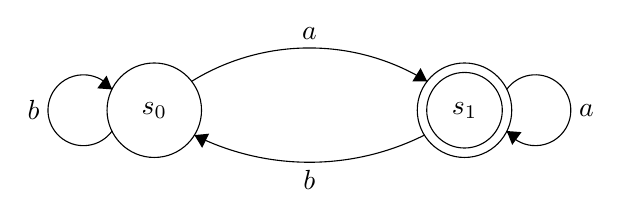
\begin{tikzpicture}[scale=0.2]
                \tikzstyle{every node}+=[inner sep=0pt]
                \draw [black] (18.2,-15.6) circle (3);
                \draw (18.2,-15.6) node {$s_0$};
                \draw [black] (37.9,-15.6) circle (3);
                \draw (37.9,-15.6) node {$s_1$};
                \draw [black] (37.9,-15.6) circle (2.4);
                \draw [black] (20.569,-13.768) arc (121.67786:58.32214:14.246);
                \fill [black] (35.53,-13.77) -- (35.11,-12.92) -- (34.59,-13.77);
                \draw (28.05,-11.15) node [above] {$a$};
                \draw [black] (35.355,-17.18) arc (-63.43003:-116.56997:16.331);
                \fill [black] (20.75,-17.18) -- (21.24,-17.99) -- (21.68,-17.09);
                \draw (28.05,-19.4) node [below] {$b$};
                \draw [black] (40.58,-14.277) arc (144:-144:2.25);
                \draw (45.15,-15.6) node [right] {$a$};
                \fill [black] (40.58,-16.92) -- (40.93,-17.8) -- (41.52,-16.99);
                \draw [black] (15.52,-16.923) arc (324:36:2.25);
                \draw (10.95,-15.6) node [left] {$b$};
                \fill [black] (15.52,-14.28) -- (15.17,-13.4) -- (14.58,-14.21);
            \end{tikzpicture}
        \end{center}


        $$\mathcal{A}_r:$$
        \begin{center}
            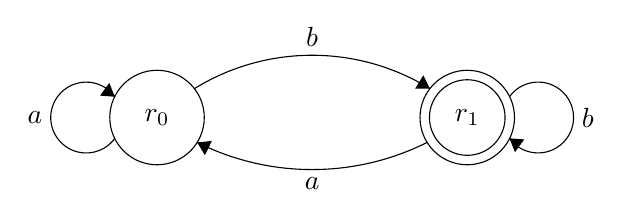
\begin{tikzpicture}[scale=0.2]
                \tikzstyle{every node}+=[inner sep=0pt]
                \draw [black] (18.2,-15.6) circle (3);
                \draw (18.2,-15.6) node {$r_0$};
                \draw [black] (37.9,-15.6) circle (3);
                \draw (37.9,-15.6) node {$r_1$};
                \draw [black] (37.9,-15.6) circle (2.4);
                \draw [black] (20.569,-13.768) arc (121.67786:58.32214:14.246);
                \fill [black] (35.53,-13.77) -- (35.11,-12.92) -- (34.59,-13.77);
                \draw (28.05,-11.15) node [above] {$b$};
                \draw [black] (35.355,-17.18) arc (-63.43003:-116.56997:16.331);
                \fill [black] (20.75,-17.18) -- (21.24,-17.99) -- (21.68,-17.09);
                \draw (28.05,-19.4) node [below] {$a$};
                \draw [black] (40.58,-14.277) arc (144:-144:2.25);
                \draw (45.15,-15.6) node [right] {$b$};
                \fill [black] (40.58,-16.92) -- (40.93,-17.8) -- (41.52,-16.99);
                \draw [black] (15.52,-16.923) arc (324:36:2.25);
                \draw (10.95,-15.6) node [left] {$a$};
                \fill [black] (15.52,-14.28) -- (15.17,-13.4) -- (14.58,-14.21);
            \end{tikzpicture}
        \end{center}


        \begin{itemize}
            \item automat rozpoznający język $r + s$:\\
            \noindent $s_{0x} = \{s_{0s}, s_{0r}\}$ \\
            \noindent $S_x = S_s \times S_r$ \\
            \noindent $f_x(\{s, r\}, a) = \{f_s(s, a), f_r(r, a)\}$ \\
            \noindent $T_x \ni t_x = \{s, r\} \Leftrightarrow s \in T_s \lor r \in T_R$ \\
            \begin{center}
                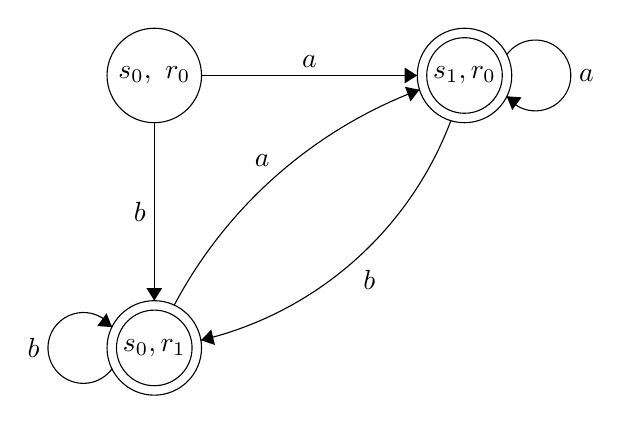
\begin{tikzpicture}[scale=0.2]
                    \tikzstyle{every node}+=[inner sep=0pt]
                    \draw [black] (18.2,-15.6) circle (3);
                    \draw (18.2,-15.6) node {$s_0,\mbox{ }r_0$};
                    \draw [black] (37.9,-15.6) circle (3);
                    \draw (37.9,-15.6) node {$s_1,r_0$};
                    \draw [black] (37.9,-15.6) circle (2.4);
                    \draw [black] (18.2,-32.9) circle (3);
                    \draw (18.2,-32.9) node {$s_0,r_1$};
                    \draw [black] (18.2,-32.9) circle (2.4);
                    \draw [black] (21.2,-15.6) -- (34.9,-15.6);
                    \fill [black] (34.9,-15.6) -- (34.1,-15.1) -- (34.1,-16.1);
                    \draw (28.05,-15.1) node [above] {$a$};
                    \draw [black] (18.2,-18.6) -- (18.2,-29.9);
                    \fill [black] (18.2,-29.9) -- (18.7,-29.1) -- (17.7,-29.1);
                    \draw (17.7,-24.25) node [left] {$b$};
                    \draw [black] (40.58,-14.277) arc (144:-144:2.25);
                    \draw (45.15,-15.6) node [right] {$a$};
                    \fill [black] (40.58,-16.92) -- (40.93,-17.8) -- (41.52,-16.99);
                    \draw [black] (15.52,-34.223) arc (324:36:2.25);
                    \draw (10.95,-32.9) node [left] {$b$};
                    \fill [black] (15.52,-31.58) -- (15.17,-30.7) -- (14.58,-31.51);
                    \draw [black] (19.468,-30.182) arc (152.05115:110.52628:29.234);
                    \fill [black] (35.04,-16.51) -- (34.12,-16.32) -- (34.47,-17.25);
                    \draw (25.05,-21.43) node [above] {$a$};
                    \draw [black] (37.033,-18.47) arc (-20.6381:-76.78447:22.448);
                    \fill [black] (21.16,-32.41) -- (22.05,-32.71) -- (21.82,-31.74);
                    \draw (31.85,-27.91) node [below] {$b$};
                \end{tikzpicture}
            \end{center}

            \item automat rozpoznający język $sr$:\\
            \noindent $s_{0x} = \{s_{0s}, \emptyset\}$ \\
            \noindent $S_x = (S_s \times \mathcal{P}(S_r))$\\
            \noindent $f_x(\{s, rs\}, a) = \{s_t, \bigcup\limits_{r \in rs}f_r(r)\}$ \\
            \noindent $f_s(s, a) = s_t \in T_s \rightarrow f_x(\{s, rs\}) = \{f_s(s, a), \{r_0\} \cup \bigcup\limits_{r \in rs}f_r(r, a)\}  $ \\
            \noindent $\{s, rs\} = t_x \in T_x \Leftrightarrow rs \cap T_r \neq \emptyset$ \\
            \begin{center}
                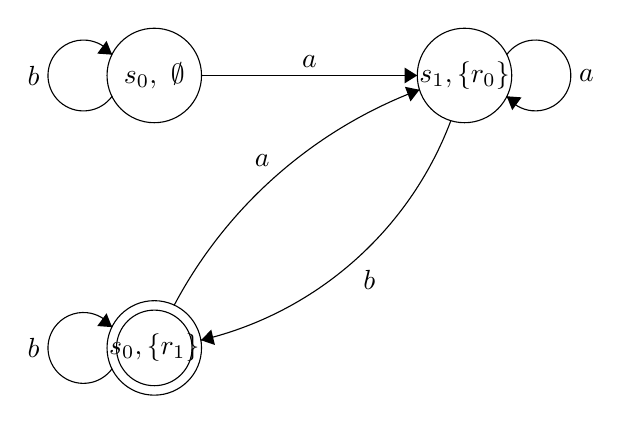
\begin{tikzpicture}[scale=0.2]
                    \tikzstyle{every node}+=[inner sep=0pt]
                    \draw [black] (18.2,-15.6) circle (3);
                    \draw (18.2,-15.6) node {$s_0,\mbox{ }\emptyset$};
                    \draw [black] (37.9,-15.6) circle (3);
                    \draw (37.9,-15.6) node {$s_1,\{r_0\}$};
                    \draw [black] (18.2,-32.9) circle (3);
                    \draw (18.2,-32.9) node {$s_0,\{r_1\}$};
                    \draw [black] (18.2,-32.9) circle (2.4);
                    \draw [black] (21.2,-15.6) -- (34.9,-15.6);
                    \fill [black] (34.9,-15.6) -- (34.1,-15.1) -- (34.1,-16.1);
                    \draw (28.05,-15.1) node [above] {$a$};
                    \draw [black] (40.58,-14.277) arc (144:-144:2.25);
                    \draw (45.15,-15.6) node [right] {$a$};
                    \fill [black] (40.58,-16.92) -- (40.93,-17.8) -- (41.52,-16.99);
                    \draw [black] (15.52,-34.223) arc (324:36:2.25);
                    \draw (10.95,-32.9) node [left] {$b$};
                    \fill [black] (15.52,-31.58) -- (15.17,-30.7) -- (14.58,-31.51);
                    \draw [black] (19.468,-30.182) arc (152.05115:110.52628:29.234);
                    \fill [black] (35.04,-16.51) -- (34.12,-16.32) -- (34.47,-17.25);
                    \draw (25.05,-21.43) node [above] {$a$};
                    \draw [black] (37.033,-18.47) arc (-20.6381:-76.78447:22.448);
                    \fill [black] (21.16,-32.41) -- (22.05,-32.71) -- (21.82,-31.74);
                    \draw (31.85,-27.91) node [below] {$b$};
                    \draw [black] (15.52,-16.923) arc (-36:-324:2.25);
                    \draw (10.95,-15.6) node [left] {$b$};
                    \fill [black] (15.52,-14.28) -- (15.17,-13.4) -- (14.58,-14.21);
                \end{tikzpicture}
            \end{center}

            \item automat rozpoznający język $r^*$:
            \noindent $s_{0x} = s_{0r}$\\
            \noindent $f_x(r, a) = f_r(r)$ \\
            \noindent $f_x(r_t \in R_t, 1) = r_{0x}$ \\
            \noindent $T_x = r_{0x}$ \\
        \end{itemize}
    \end{itemize}
    \newpage

    \section{Automaty niedeterministyczne i deterministyczne (w tym ze stosem); determinizacja.}

    \subsection{Determinizacja automatów skończenie stanowych}

    \begin{theorem}
        Język $L \in A^*$ jest rozpoznawany przez automat deterministyczny wtedy
        i tylko wtedy, gdy jest rozpoznawany przez automat niedeterministyczny.
    \end{theorem}

    $\mathcal{A}_{ND} = (S, f, I, F)$ - automat niedeterministyczny\\
    \indent$\mathcal{A}_D = (P(S), \overline{f}, I, T)$ - równoważny automat deterministyczny, gdzie:
    $$\overline{f} : P(S) \times A^* \rightarrow P(S)$$
    $$\forall Q \in P(S), \forall w \in A^* \; \; \overline{f}(Q, w) = \bigcup\limits_{s \in Q} f(s, w)$$
    $$T = \{Q \in P(S) | Q \cap F \neq \emptyset\}$$

    \subsection{Determinizm automatu ze stosem}

    \begin{definition}
        \textbf{Deterministyczny automat ze stosem}

        Automatem $\mathcal{AS} = (A, A_S, Q, q_0, z_0, f, Q_F)$ nazywamy
        \textbf{deterministycznym}, jeśli dla każdej konfiguracji
        $(z, q, a) \in A_S^* \times Q \times (A \cup \{1\})$
        $$f(z, q, a) \leq 1 \; \mathrm{oraz}$$
        $$f(z, q) \neq \emptyset \Rightarrow f(z, q, a) = \emptyset \; \forall a \in A$$
        Język akceptowany przez automat deterministyczny nazywamy językiem deterministycznym.
    \end{definition}

    \begin{theorem}
        Każdy język deterministyczny jest jednoznaczny (rozpoznawany przez gramatykę jednoznaczną), ale nie na odwrót.
    \end{theorem}

    \begin{theorem}
        Każdy język deterministyczny jest kontekstowy (rozpoznawany przez niedeterministyczny automat ze stosem), ale nie na odwrót.
    \end{theorem}

    \newpage

    \section{Problemy rozstrzygalne i nierozstrzygalne w teorii języków.}

    Problemy rozpatrywane w kategorii języków
    \begin{itemize}
        \item Należenie $\in$ - Problem przynależności języka $L$ do jednego z typów języków $L_i$ gdzie $i \in {0,1,2,3}$ generowanych przez odpowiednie gramatyki  $G_i$
        \item Inkluzja $\subset$ - Problem zawierania się języka $L_i$ w języku $L_k$
        \item Równoważność $\equiv$ - Problem równoważności dwóch języków $L_1 \equiv L_2$
        \item Pustość $\emptyset$ - Problem języka pustego czyli nie generującego żadnego słowa
        \item Nieskończonośc $\infty$ - Problem języka nieskończonego czyli generującego nieskończenie wiele słów
        \item Jednoznaczność
    \end{itemize}

    \begin{definition}
        Wyprowadzenie lewostronne (prawostronne)

        Niech $G = (V_N,V_T,v_0,P)$ będzie gramatyką bezkontekstową.

        Lewostronnym (prawostronnym) wyprowadzeniem słowa $w \in {V_T}^\star$ w gramatyce $G$ nazywamy wyprowadzenie
        $v_0 \mapsto w_1 \mapsto \ldots.. \mapsto w_n = w$
        takie, że dla każdego $i=0,\ldots,n-1, \;\; w_{i+1}$ jest generowane bezpośrednio z $w_i$ przez zastąpienie pierwszego z lewej (prawej) symbolu nieterminalnego występującego w słowie $w_i$.
        Jeśli chcemy zaznaczyć, że wyprowadzenie jest lewostronne lub prawostronne, to posługujemy się zapisem

        $v_{0}\mapsto_{L}^{*}w,\; v_{0}\mapsto_{P}^{\star}w$.
    \end{definition}

    \begin{definition}
        Jednoznaczność -

        Gramatyka bezkontekstowa $G$ jest \textbf{jednoznaczna} $\Leftrightarrow$ każde słowo generowane przez tę gramatykę ma \textbf{dokładnie jedno wyprowadzenie lewostronne (prawostronne)}.

        Język bezkontekstowy $L$ nazywamy \textbf{jednoznacznym}, jeśli istnieje jednoznaczna gramatyka bezkontekstowa generująca ten język.

        Jednoznaczność gramatyki oznacza istnienie dokładnie jednego drzewa wywodu dla każdego generowanego słowa.
    \end{definition}


    \begin{center}
        \begin{tabular}{||c c c c c||}
            \hline
            --- & 3 & 2 & 1 & 0 \\ [0.5ex]
            \hline\hline
            Należenie $\in$ & T & T & T & N \\
            \hline
            Inkluzja $\subset$ & T & N & N & N \\
            \hline
            Równoważność $\equiv$ & T & N & N & N \\
            \hline
            Pustość $\emptyset$ & T & T & N & N \\
            \hline
            Nieskończoność $\infty$ & T & T & N & N \\
            \hline
            Jednoznaczność & T & N & - & - \\ [1ex]
            \hline
        \end{tabular}
    \end{center}

    Oznaczenia\\
    T - rozstrzygalny\\
    N - nieroztrzygalny

    \newpage


    \section{Klasy języków w hierarchii Chomsky’ego oraz ich zamkniętość ze względu na operacje boolowskie, homomorfizmy, itp.}

    \begin{definition}
        Gramatyka

        Jest to system $G=(V_N,V_T,P,v_0)$, w którym
        \begin{itemize}
            \item
            $V_N \ne \emptyset$ - skończony zbiór symboli nieterminalnych (alfabet nieterminalny)
            \item
            $V_T \ne \emptyset$ - skończony zbiór symboli terminalnych (alfabet terminalny)
            \item
            $P \subseteq (V_N \cup V_T)^+ \times (V_N \cup V_T)^\star$ - skończona relacja, zbiór produkcji (praw)
            \item
            $v_0 \in V_N$ - symbol początkowy (startowy)
        \end{itemize}

        Ponadto zakładamy, że $V_N \cap V_T = \emptyset$ i dla każdego
        $(u,v)\in P$; $\#_{V_N} u >= 1$

        Zatem w gramatyce alfabety terminalny i nieterminalny są rozłącznymi zbiorami, a słowo u występujące po lewej stronie produkcji zawiera co najmniej jeden symbol nieterminalny. Fakt, że para $(u,v) \in P$, zapisujemy:

        $u \rightarrow v \in P$ lub $u \rightarrow_G v$.

        Wykorzystujemy też zdefiniowane dla systemów przepisujących pojęcia generowania bezpośredniego "$\mapsto$" i generowania "$\mapsto \star$".
    \end{definition}

    \begin{definition}
        Gramatyka $G=(V_N,V_T,P,v_0)$ jest typu (i) dla $i=0,1,2,3$ wtedy i tylko wtedy, gdy spełnia następujące warunki:

        \begin{itemize}
            \item Gramatyka

            Każdy system spełniajacy definicję 57.1
            \item Kontekstowa

            Gramatyka, w której każde prawo ze zbioru P ma postać $u_1vu_2 \rightarrow u_1xu_2$

            gdzie $u_1,u_2 \in (VN \cup VT)^\star,v \in V_N,x \in (V_N \cup V_T)^+$ lub $v_0 \rightarrow 1$,przy czym, jeśli $v_0 \rightarrow 1 \in P$, to $v_0$ nie występuje po prawej stronie w żadnym prawie z $P$

            \item Bezkontekstowa

            Gramatyka, w której każde prawo ze zbioru P ma postać
            $v \rightarrow x$

            gdzie $v \in V_N, x \in (V_N \cup V_T)^\star$

            \item Regularna

            Gramatyka, w której każde prawo ze zbioru P ma postać
            $v \rightarrow v'x$ lub $v \rightarrow x$

            gdzie $v,v' \in V_N$;$x \in V_T^\star$
            \\


            W oparciu o wprowadzone typy gramatyk określamy odpowiadające im rodziny (klasy) języków, oznaczając przez

            $\bf \mathcal{L}_{0}$ rodzinę wszystkich języków typu 0

            $\bf \mathcal{L}_{1}$ rodzinę wszystkich języków typu 1 - kontekstowych

            $\bf \mathcal{L}_{2}$ rodzinę wszystkich języków typu 2 - bezkontekstowych

            $\bf \mathcal{L}_{3}$ rodzinę wszystkich języków typu 3 - regularnych

            Pomiędzy wprowadzonymi rodzinami języków zachodzą następujące zależności:

            $\bf \mathcal{L}_{3}\subseteq \! \! \! \! \! _{/\; \, }\bf \mathcal{L}_{2}\subseteq \! \! \! \! \! _{/\; \, }\bf \mathcal{L}_{1}\subseteq \! \! \! \! \! _{/\; \, }\bf \mathcal{L}_{0}$

        \end{itemize}

    \end{definition}

    Zamkniętości języków na operacje
    \begin{center}
        \begin{tabular}{||c c c c c||}
            \hline
            --- & 3 & 2 & 1 & 0 \\ [0.5ex]
            \hline\hline
            $\cup$ & T & T & T & T \\
            \hline
            $\cdot$ & T & T & T & T \\
            \hline
            $\star$ & T & T & T & T \\
            \hline
            $\setminus$ & T & N & T & N \\
            \hline
            $\cap $ & T & N & T & T \\ [1ex]
            \hline
        \end{tabular}
    \end{center}

    \newpage

    {\Large Wytwarzanie oprogramowania}

    \section{Reprezentacja liczb całkowitych; arytmetyka.}

    \subsection{Kod znak-moduł prosty}
    \subsubsection{Reguły:}
    \begin{enumerate}
        \item Sygnalizacja znaku poprzez najwyższą pozycję
        rejestru (najczęściej pierwszą pozycję od lewej).
        \item Cyfra 0 na pozycji znaku oznacza dodatniość.
        \item Niezerowa cyfra na pozycji znaku oznacza ujemność.
        \item Cyfry określające wartość liczby (pozostałe cyfry) bez zmian (bez żadnego kodowania).
    \end{enumerate}
    \subsubsection{Przykłady:}
    \begin{itemize}
        \item Przykład w systemie dziesiętnym, q = 10,
        c = 5, u = 2, n = 8.\\
        $[+216.7]_{zmp} = 0|00216.70$\\
        $[-216.7]_{zmp} = 1|00216.70$
        \item Przykład w systemie binarnym, q = 2, c = 10,
        u = 5, n = 16.\\
        $[+1001100.101]_{zmp} = 0|0000100110.10100$\\
        $[-1001100.101]_{zmp} = 1|0000100110.10100$
    \end{itemize}
    \subsubsection{Arytmetyka}
    Kodowanie znak-moduł prosty przez swoją skomplikowaną
    i czasochłonną arytmetykę nie nadaje się do praktycznego
    stosowania (konieczność niestandardowego obsługiwania przepełnień)

    \subsection{Kod odwrotnościowy}
    \subsubsection{Reguły}
    \begin{itemize}
        \item Najbardziej znacząca cyfra (najczęściej lewa) jest cyfrą znaku.
        \item Zerowa cyfra znaku oznacza dodatniość.
        \item Najwyższa (ostatnia) cyfra znaku oznacza ujemność.
        \item Cyfry wartości liczby dodatniej pozostają bez zmian
        \item Cyfry wartości dla liczby ujemnej:
        \begin{itemize}
            \item W systemie dwójkowym są odwróceniem bitów.
            \item W systemie dziesiętnym są uzupełnieniem każdej cyfry
            do liczby 9.
            \item Ogólnie są uzupełnienie każdej cyfry do najwyższej cyfry
            systemu, czyli do wartości q-1.
        \end{itemize}
    \end{itemize}

    \subsubsection{Przykłady}
    \begin{itemize}
        \item System dziesiętny:
        q = 10, c = 7, u = 5
        \begin{align*}
        [-182073.6954]
            _{odw} = [-0|0182073.69540]_{odw} = 9|9917926.30459
        \end{align*}

        \item - System binarny:
        q = 2, c = 7, u = 5
        \begin{align*}
        [-101110.011]
            _{odw} = [-0|0101110.01100]_{odw} = 1|0010001.10011
        \end{align*}

    \end{itemize}

    \subsubsection{Arytmetyka}
    Algorytm sumowania:
    \begin{itemize}
        \item Dodaj kody, a w przypadku przepełnienia zwiększ wynik o najmniejszą możliwą liczbę dodatnią.
    \end{itemize}

    \subsubsection{Przykłady}
    \begin{itemize}
        \item W systemie dzisiętnym, q=10, c=7, u=5
        \begin{center}
            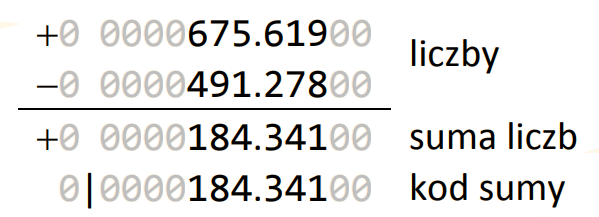
\includegraphics[scale=0.4]{graphics/number-repr/odw-add-dec.png}
        \end{center}
        \begin{center}
            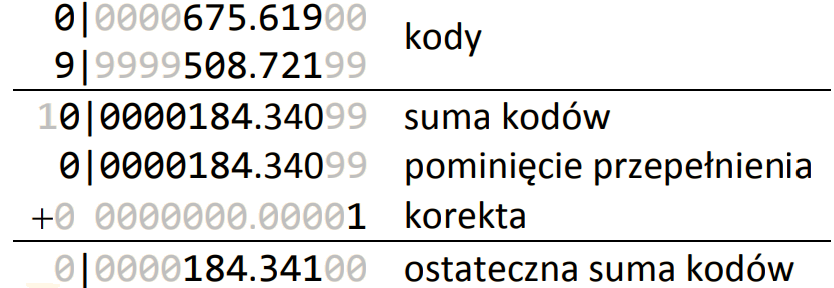
\includegraphics[scale=0.4]{graphics/number-repr/odw-add-dec-2.png}
        \end{center}


        \item w systemie binarnym, q=2, c=7, u=5
        \begin{center}
            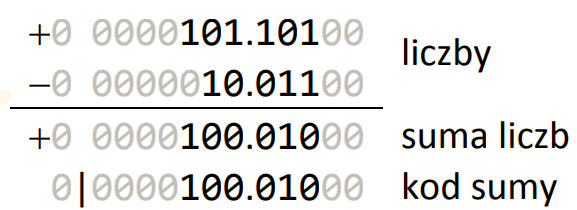
\includegraphics[scale=0.4]{graphics/number-repr/odw-add-bin.png}
        \end{center}
        \begin{center}
            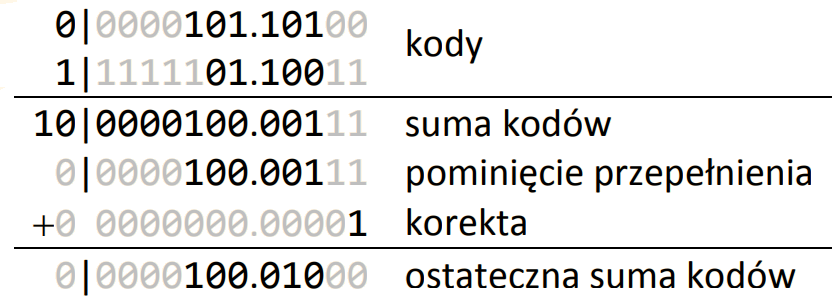
\includegraphics[scale=0.4]{graphics/number-repr/odw-add-bin-2.png}
        \end{center}

    \end{itemize}


    \subsection{Kod uzupełnieniowy}
    \subsubsection{Kodowanie}
    Kodowanie uzupełnieniowe liczby ujemnej polega na uzupełnieniu każdej cyfry do najwyższej
    cyfry systemu (odwróceniu bitów) i dodaniu do
    otrzymanej wartości liczby 1 na najmniej znaczącym miejscu.
    \subsubsection{Dekodowanie}
    Dekodowanie liczby ujemnej zakodowanej uzupełnieniowo polega na odjęciu od kodu liczby 1
    na najmniej znaczącym miejscu z uzupełnieniem
    w otrzymanym kodzie każdej cyfry do najwyższej
    cyfry systemu (odwróceniem bitów).

    \subsubsection{Przykłady kodowania}
    \begin{itemize}
        \item w systemie dziesiętnym (q = 10, c = 7, u = 5)
        \begin{center}
            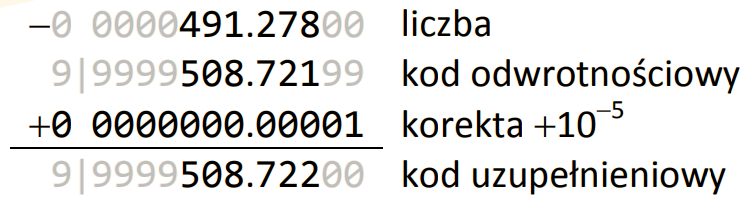
\includegraphics[scale=0.4]{graphics/number-repr/uzp-encode-dec.png}

        \end{center}
        \item w systemie binarnym q = 10, c = 7, u = 5.
        \begin{center}
            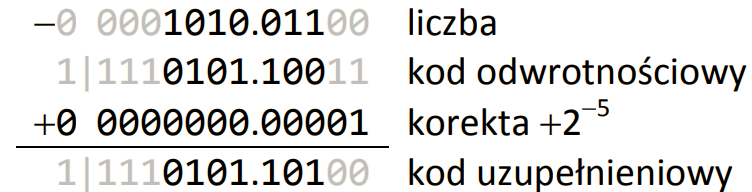
\includegraphics[scale=0.4]{graphics/number-repr/uzp-encode-bin.png}
        \end{center}

    \end{itemize}

    \subsubsection{Arytmetyka}
    Suma kodów uzupełnieniowych jest zawsze kodem uzupełnieniowym sumy.
    \begin{itemize}
        \item w systemie dziesiętnym  (q = 10, c = 7, u = 5)
        \begin{center}
            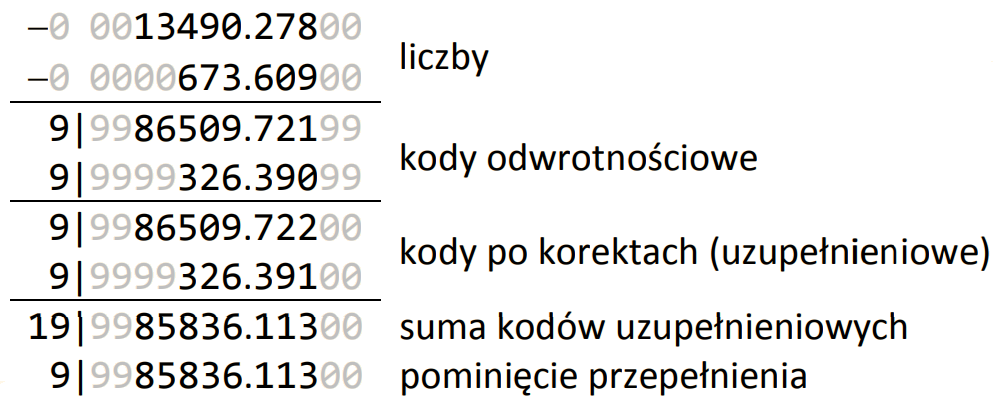
\includegraphics[scale=0.4]{graphics/number-repr/uzp-add-dec.png}
        \end{center}

        \item w systemie binarnym q = 10, c = 7, u = 5
        \begin{center}
            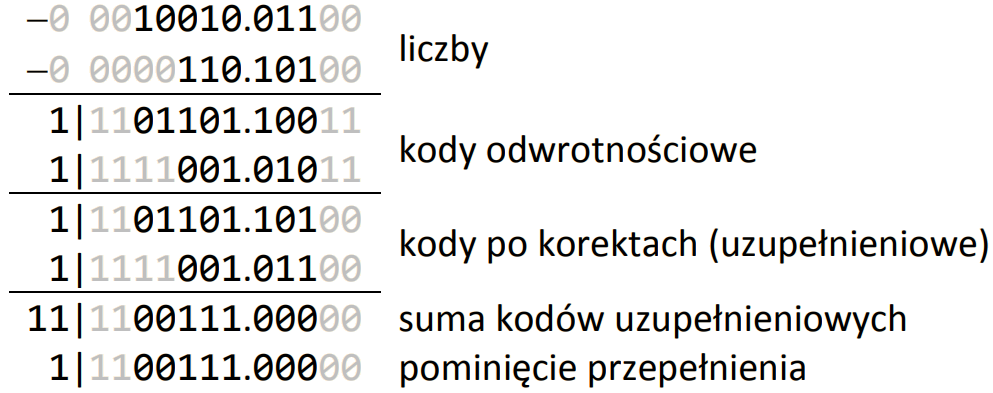
\includegraphics[scale=0.4]{graphics/number-repr/uzp-add-bin.png}
        \end{center}
    \end{itemize}

    \subsection{Kod nadmiarowy}
    \subsubsection{Kodowanie}
    \begin{enumerate}
        \item Kodowanie nadmiarowe liczby dodatniej polega na
        ustawieniu cyfry znaku na wartość jednostkową.
        \begin{center}
            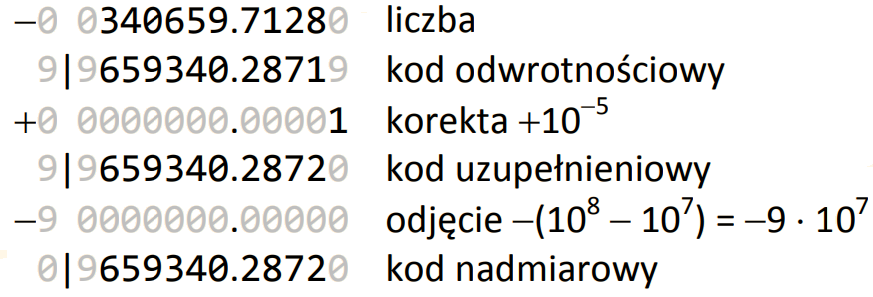
\includegraphics[scale=0.4]{graphics/number-repr/nad-encode-dec.png}
        \end{center}
        \item Kod nadmiarowy liczby ujemnej to kod uzupełnieniowy z odjęciem najwyższej cyfry systemu
        na pozycji znaku.
        \begin{center}
            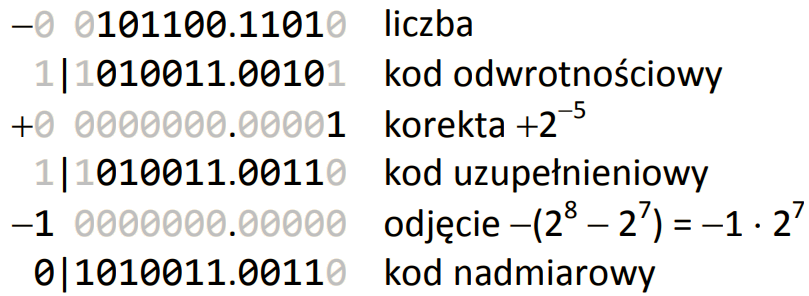
\includegraphics[scale=0.4]{graphics/number-repr/nad-encode-bin.png}
        \end{center}
    \end{enumerate}


    \subsubsection{Deokodowanie}
    \begin{itemize}
        \item Dekodowanie nadmiarowe kodu liczby dodatniej
        (rozpoznawanego po niezerowej cyfrze znaku) polega na wyzerowaniu cyfry znaku.
        \item Dekodowanie nadmiarowe kodu liczby ujemnej
        (rozpoznawanego po zerowej cyfrze znaku) wymaga
        ustawienia najwyższej cyfry systemu w miejscu znaku z następującym dekodowaniem uzupełnieniowym.
    \end{itemize}

    \subsubsection{Arytmetyka}
    Kod nadmiarowy sumy liczb to suma kodów nadmiarowych
    składników z odjętą wartością 1 na pozycji znaku.

    \begin{enumerate}
        \item w systemie dziesiętnym
        \begin{center}
            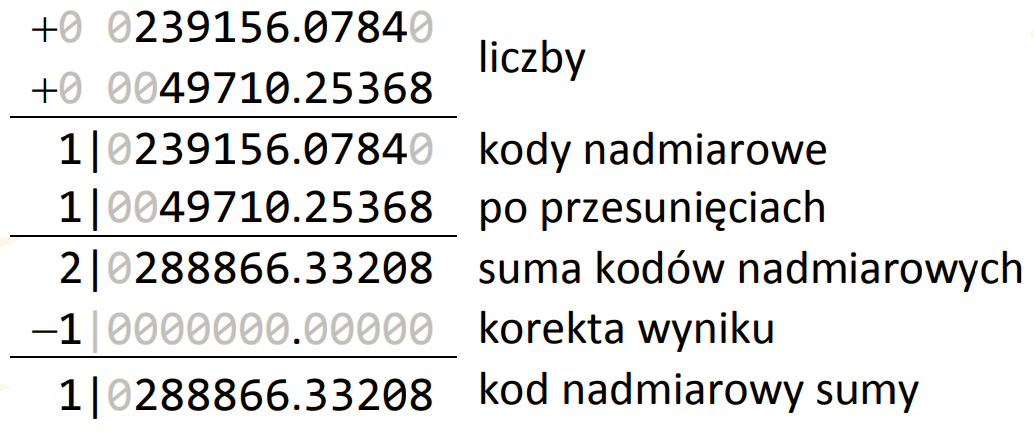
\includegraphics[scale=0.4]{graphics/number-repr/nad-add-dec.png}
        \end{center}
        \begin{center}
            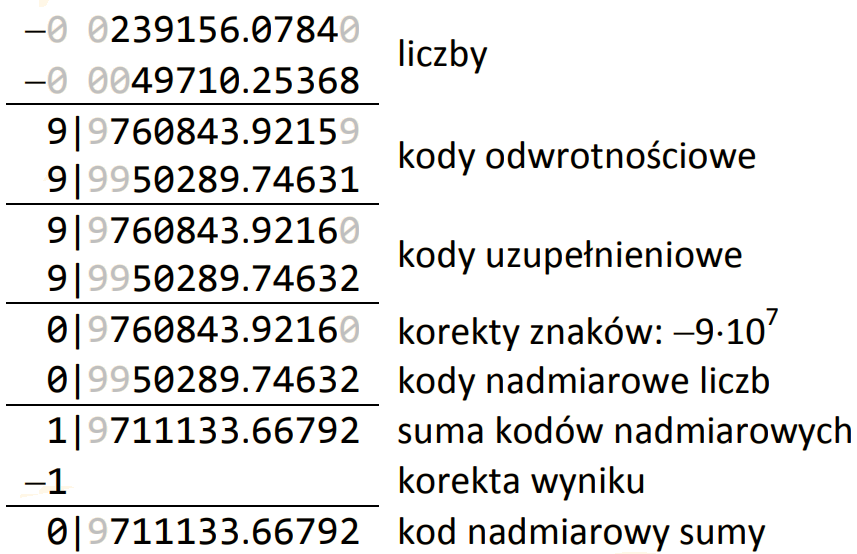
\includegraphics[scale=0.4]{graphics/number-repr/nad-add-dec-2.png}
        \end{center}

        \item w systemie binarnym
        \begin{center}
            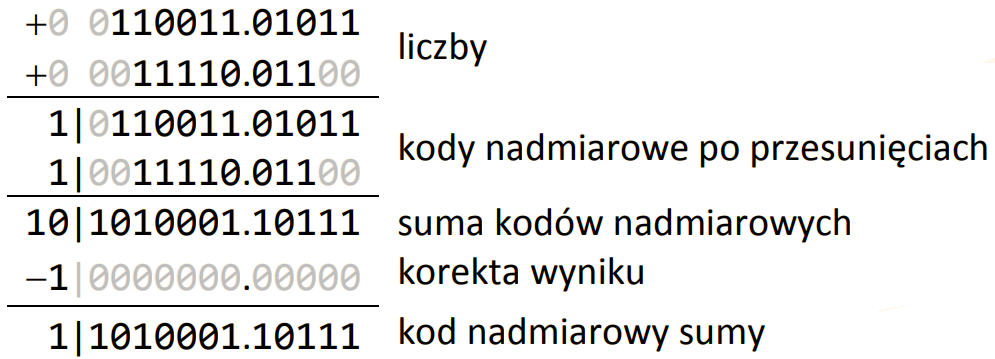
\includegraphics[scale=0.4]{graphics/number-repr/nad-add-bin.png}
        \end{center}
        \begin{center}
            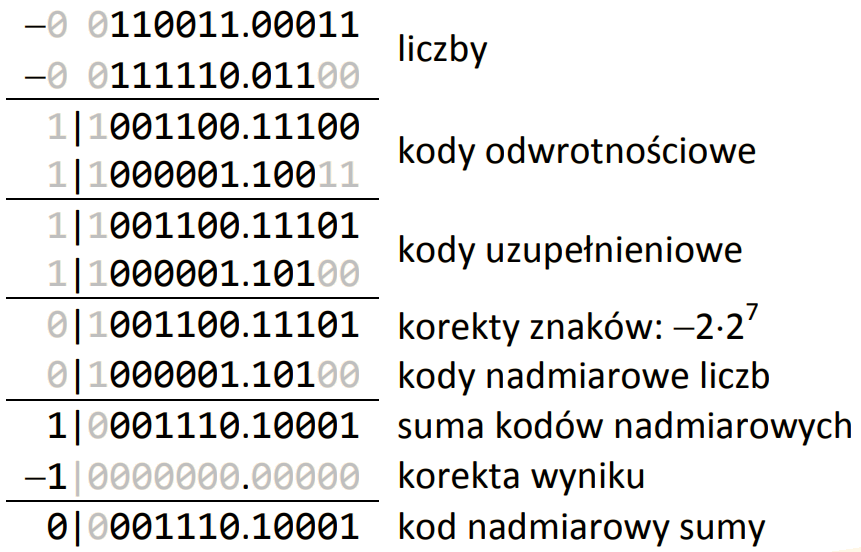
\includegraphics[scale=0.4]{graphics/number-repr/nad-add-bin-2.png}
        \end{center}
    \end{enumerate}






    \newpage

    \section{Reprezentacja liczb rzeczywistych; arytmetyka zmiennopozycyjna.}

    \subsection{Reprezentacja cecha-mantysa}
    Liczby postaci
    \begin{align*}
        m \times q^c
    \end{align*}
    gdzie m - mantysa, q - podstawa systemu liczbowego, c - cecha

    \begin{itemize}
        \item Mantysa - ciąg najbardziej znaczących cyfr liczby.
        \item Cecha - wykładnik potęgi podstawy systemu w iloczynie z mantysą równy reprezentowanej liczbie.
        \item W rejestrze komputera pamiętane są wyłącznie mantysa oraz cecha, zaś podstawa systemu jest ustalona, zatem nie musi być reprezentowana i nie jest konieczna do działań.
        \item Różnorodne sposoby zapamiętania w komputerze liczb w postaci cecha-mantysą noszą nazwę \textbf{kodowań zmiennopozycyjnych.}

    \end{itemize}

    \subsection{Kodowanie zmiennopozycyjne}
    \begin{itemize}
        \item Kodowanie zmiennopozycyjne jest powszechnie stosowanie w komputerach dla reprezentacji liczb rzeczywistych.
        \item W systemie dziesiętnym dla oddzielenia mantysy i cechy powszechne użycie litery E (lub e).
        Liczba 28.05
        \begin{center}
            \texttt{28.05e0 = 2805e-2 = +2805000e-5 =\\
            = 0.0002805e+5 = 2.805e1 = 0.2805e2}
        \end{center}

        \item W systemie binarnym dla oddzielenia mantysy i cechy powszechne użycie litery D (lub d).
        Liczba $(9.625)_{10} = (1001.101)_2$
        \begin{center}
            \texttt{0.00001001101d1000 = 1001101000d-110 =\\
            = 1.001101d11 = 0.1001101d100}
        \end{center}

        \item Różnorodność reprezentacji zmiennopozycyjnej wymusza konieczność ujednoznacznienia zwaną \textbf{normalizacją.}

    \end{itemize}

    \subsection{Normalizacja}

    \begin{table}
        \centering
        \begin{tabular}{l|l|l|l}
            & normalizacja
            całkowita & normalizacja
            do jedynki & normalizacja
            do ułamka  \\
            \hline
            28.05 & \texttt{2805e-2}                & \texttt{2.805e1}                  & \texttt{.2805e2}                  \\
            -35000000 & -\texttt{35e6}                & -\texttt{3.5e7}                   & -\texttt{.35e8}                   \\
            0.0000576 & \texttt{576e-6}                  & \texttt{5.76e-4}                  & \texttt{.576e-3}                  \\
            \hline
            $(1001.101)_2$    & \texttt{1001101d-11}             & \texttt{1.001101d11}              & \texttt{.1001101d100}             \\
            $(1010000)_2$     & \texttt{101d100}                 & \texttt{1.01d110}                 & \texttt{.101d111}                 \\
            $(-0.00001011)_2$ & -\texttt{1011d1001}              & -\texttt{1.011d111}               & -\texttt{.1011d1000}
        \end{tabular}
    \end{table}

    \subsection{Algorytmy kodowania i dekodowania}
    Przyjmujemy oznaczenia:
    \begin{itemize}
        \item $w_m$ - liczba cyfr reprezentacji mantysy (bez cyfry znaku)
        \item $w_c$ - liczba cyfr reprezentacji cechy (bez cyfry znaku)
        \item n - liczba cyfr rejestru
    \end{itemize}
    Zatem:
    \begin{align*}
        n = 1 + w_m + 1 + w_c
    \end{align*}

    \subsubsection{Algorytm kodowania}

    Algorytm kodowania zmiennomozycyjnego obejmuje poniższe kroki:
    \begin{enumerate}
        \item Przedstaw liczbę w systemie o podstawie q.
        \item Zaokrąglij wartość liczby do $w_m$ cyfr.
        \item Zaokrąglony wynik sprowadź do znormalizowanej postaci
        potęgowej $m\cdot q^c$
        \item Jeżeli cecha jest zbyt duża (zbyt dodatnia) by zmieścić się
        w przewidzianym zakresie $w_c$ to zasygnalizuj błąd przepełnienia i zakończ.
        \item Jeżeli cecha jest zbyt mała (zbyt ujemna) by zmieścić się
        w zakresie $w_c$ to zakoduj zerową mantysy oraz zerową wartość cechy i zakończ.
        \item Zakoduj stałopozycyjnie mantysę na $w_m + 1$ pozycjach.
        \item Zakoduj stałopozycyjnie cechę na $w_c + 1$ pozycjach.
    \end{enumerate}

    Przykłady dziesiętne:

    \begin{center}
        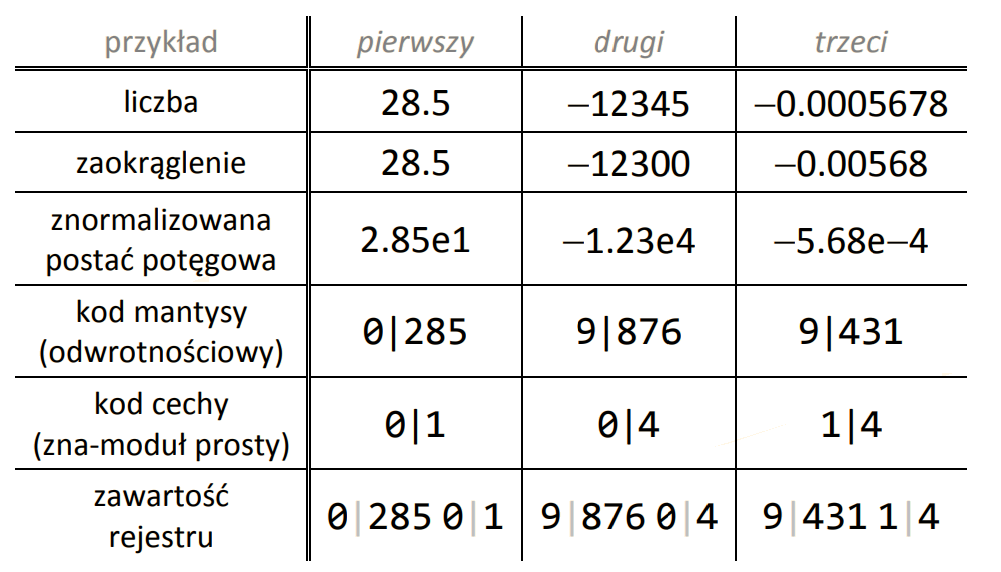
\includegraphics[scale=0.4]{graphics/number-repr/fl-pt-encode-dec.png}
    \end{center}

    Przykłady binarne:

    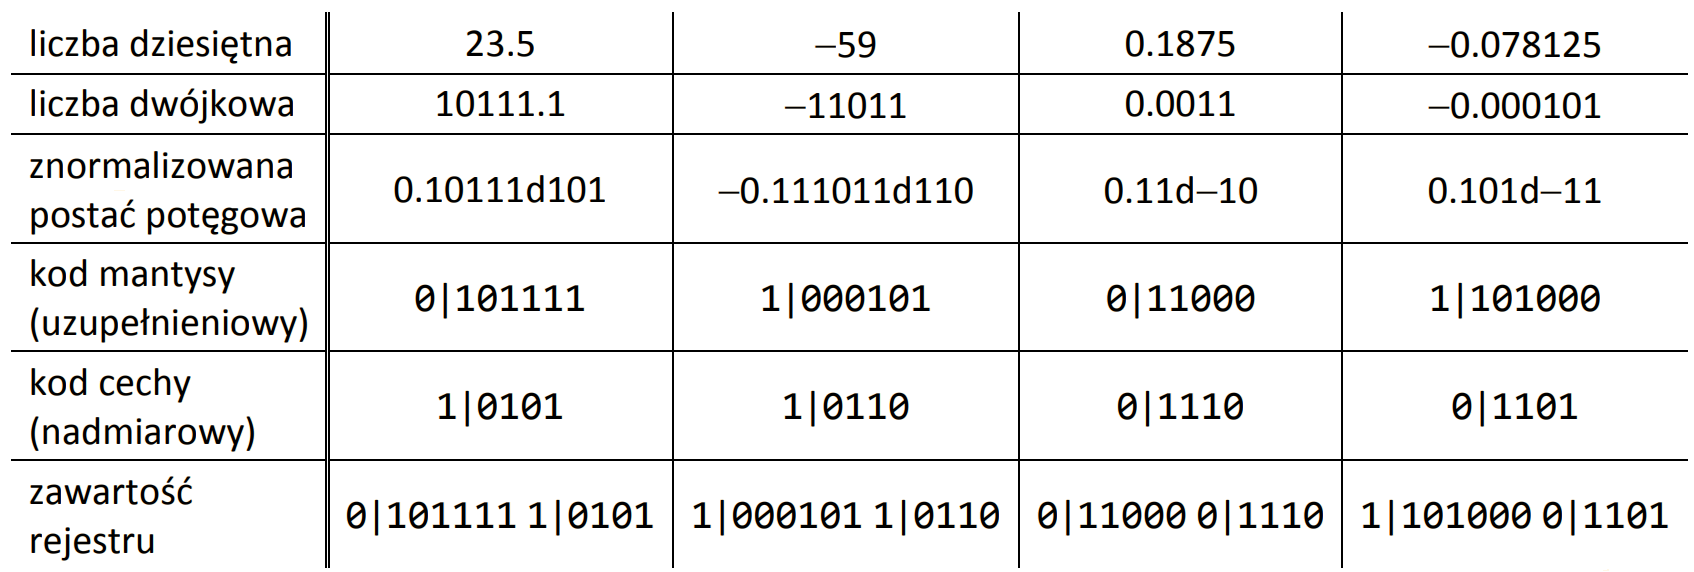
\includegraphics[width=\linewidth]{graphics/number-repr/fl-pt-encode-bin.png}

    \subsubsection{Algorytm dekodowania}

    System dziesiętny:
    \begin{enumerate}
        \item Dekoduj mantysę i cechę.
        \item Opcjonalnie eliminuj postać potęgową.
    \end{enumerate}

    System binarny:
    \begin{enumerate}
        \item Dekoduj mantysę i cechę.
        \item Sprowadź cechę do postaci dziesiętnej.
        \item Zdenormalizuj mantysę.
        \item Zapisz mantysę w postaci dziesiętnej.
    \end{enumerate}

    Przykłady binarne:

    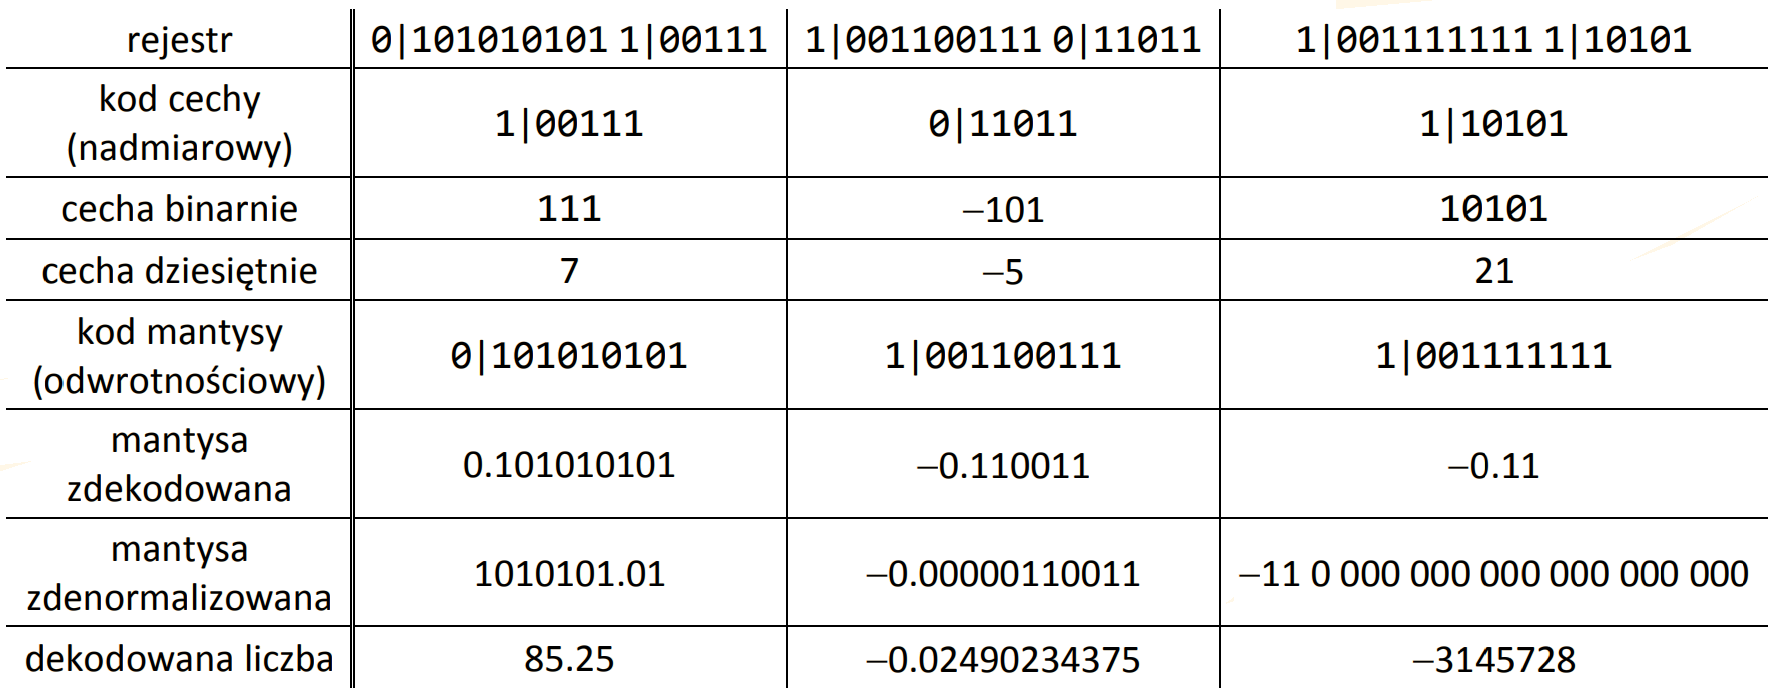
\includegraphics[width=\linewidth]{graphics/number-repr/fl-pt-decode-bin.png}

    \subsection{Arytmetyka}
    \begin{itemize}
        \item Brak ogólnego algorytmu działania na kodach
        zmiennopozycyjnych.
        \item Jedyna możliwa droga obejmuje oczywiste
        kroki:
        \begin{enumerate}
            \item Dekodowanie argumentów.
            \item Wykonanie działania.
            \item Zakodowanie wyniku.
        \end{enumerate}
    \end{itemize}

    \subsubsection{Dodawanie kodów zmiennopozycyjnych}
    Algorytm obejmuje kroki:
    \begin{enumerate}
        \item Zmodyfikuj mantysy dla zrównania cech (z możliwością
        denormalizacji).
        \item Wyznacz mantysę sumy w postaci sumy mantys (możliwe wobec równych cech).
        \item Zaokrąglij sumę mantys do liczby cyfr rejestru.
        \item Znormalizuj wynik sumy (skoryguj cechę wyniku).
    \end{enumerate}
    Przykład:\\
    \begin{center}
        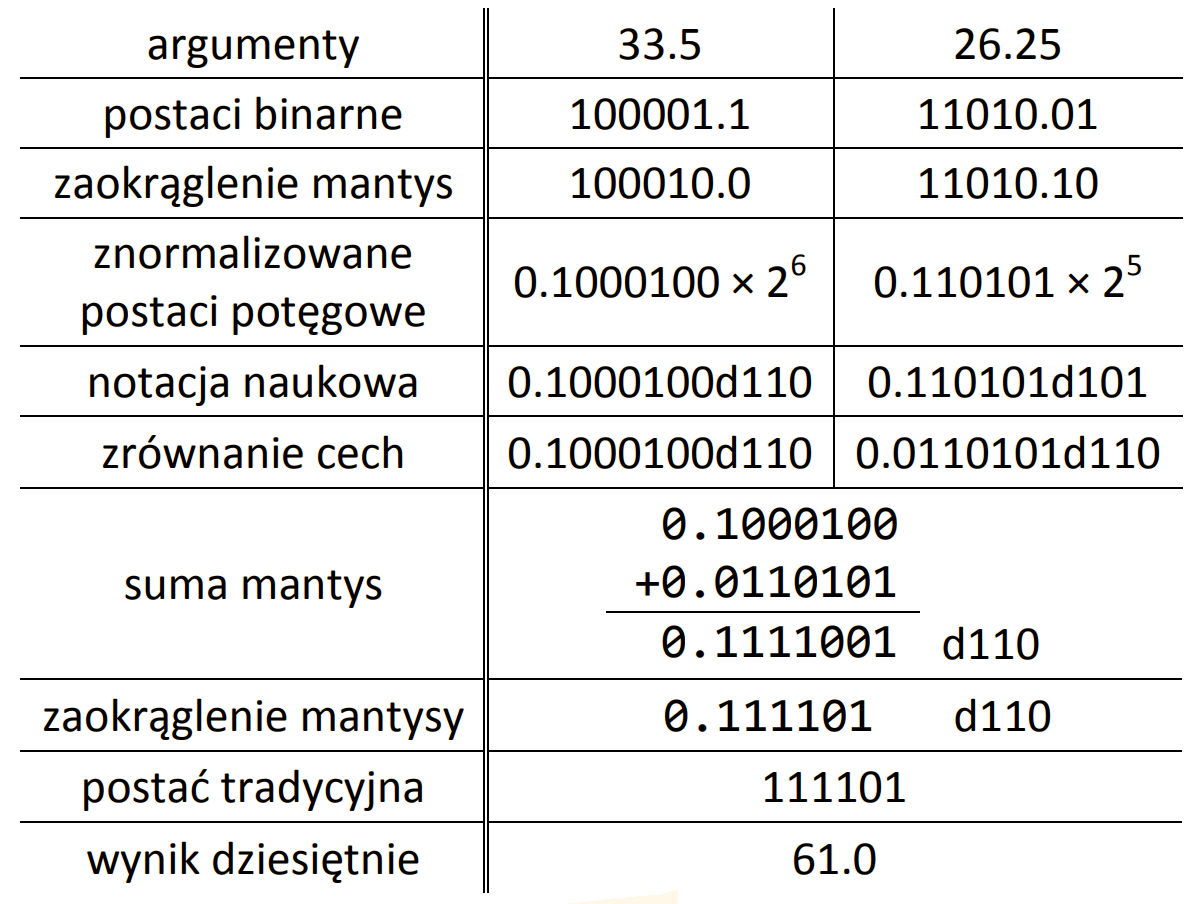
\includegraphics[scale=0.3]{graphics/number-repr/fl-pt-add.png}
    \end{center}

    \subsubsection{Mnożenie kodów zmiennopozycyjnych}
    Algorytm może obejmować kroki:
    \begin{enumerate}
        \item Mantysa iloczynu to iloczyn mantys, dlatego
        pomnóż mantysy.
        \item Cecha iloczynu to suma cech, zatem dodaj
        cechy.
        \item Zaokrąglij mantysę wyniku, iloczynu mantys.
        \item Znormalizuj mantysę modyfikując cechę.
    \end{enumerate}
    Przykład:\\
    \begin{center}
        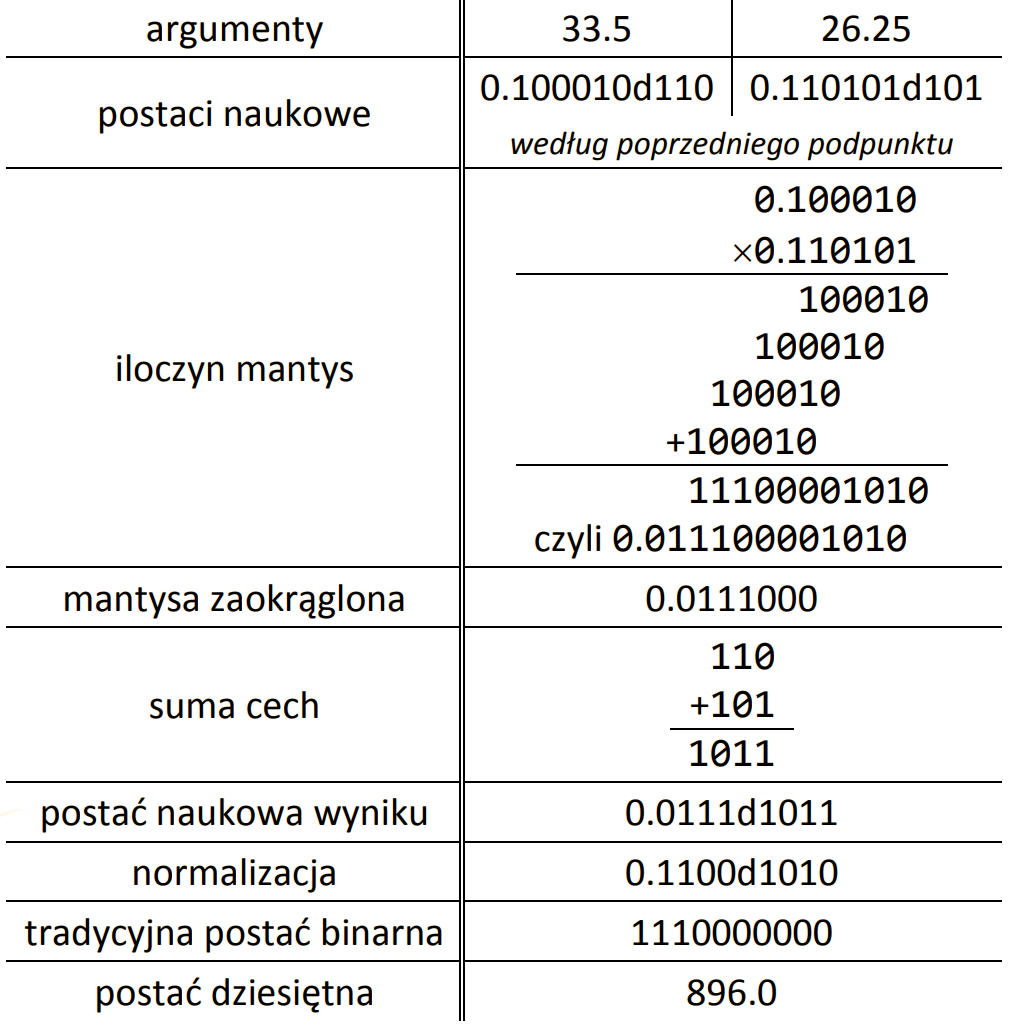
\includegraphics[scale=0.4]{graphics/number-repr/fl-pt-mult.png}
    \end{center}

    \newpage

    \section{Różnice w wywołaniu funkcji statycznych, niestatycznych i wirtualnych w C++.}

    \subsection{Funkcje statyczne.}
    \begin{itemize}
        \item \textbf{Globalne funkcje statyczne} to funkcje o zakresie widoczności ograniczonym do pliku źródłowego, który je
        zawiera (a dokładniej do ich \textit{jednostce translacji}, czyli pliku który jest kompilowany - zatem pliku
        źródłowego wraz z dołączonymi includami).
        \item \textbf{Metody statyczne klas} to metody których wywołanie jest niezależne od instancjonowania klasy -
        wszystkie instancje klasy współdzielą kopię statycznych metod i pól. Instancja klasy nie jest nam potrzebna
        do wywołania statycznej metody (aczkolwiek można jej użyć).
    \end{itemize}

    \begin{minted}{cpp}
        #include <iostream>
        using namespace std;

        // statyczna funkcja globalna dostępna tylko z naszego pliku
        static void sayHello(){
        cout << "hello" << endl;
        }

        class ExampleClass {
        public:
        static void sayBye(){
        cout << "bye" << endl;
        }
        };

        int main(){
        sayHello();

        ExampleClass::sayBye(); // wywołanie bez instancjonowania klasy

        ExampleClass e();
        e.sayBye(); // wywołanie dla instancji klasy
        }
    \end{minted}

    \subsection{Funkcje niestatyczne.}
    \begin{itemize}
        \item \textbf{Niestatyczne funkcje globalne} są dostępne ze wszystkich plików, które includują zawierające
        je plik źródłowy - trzeba zatem uważać na konflikty nazw.
        \item \textbf{Nietstatyczne metody klas} wymagają do wywołania instancji klasy - mogą zachowywać się różnie
        dla różnych instancji; mogą być oznaczone \texttt{final} i \texttt{override}.
    \end{itemize}

    \begin{minted}{cpp}
        #include <iostream>
        using namespace std;

        // niestatyczna funkcja globalna dostępna dla wszystkich plików
        void sayHello(){
        cout << "hello" << endl;
        }

        class ExampleClass {
        public:
        void sayBye(){
        cout << "bye" << endl;
        }
        };

        int main(){
        sayHello();

        // ExampleClass::sayBye() - wywołanie niepoprawne

        ExampleClass e();
        e.sayBye(); // wywołanie dla instancji klasy
        }
    \end{minted}

    \subsection{Funkcje wirtualne.}
    \begin{itemize}
        \item \textbf{Wirtualne metody klas} są przydatne polimorfiźmie.
        \item W przypadku zwykłej metody, wywołanie jej dla wskaźnika typu klasy podstawowej zawsze wywoła instancję
        z klasy podstawowej, nawet jeżeli wskaźnik będzie tak naprawdę wskazywał na klasę pochodną.
        \item Słowo kluczowe \texttt{virtual} wymusza dedukcję której metody użyć na podstawie zawartości wskaźnika,
        a nie jego typu. Dedukcja następuje w czasie wykonania programu.
    \end{itemize}

    Bez \texttt{virtual}:
    \begin{minted}{cpp}
        #include <iostream>
        using namespace std;

        struct Base {
        void f() {
        cout << "base" << endl;
        }
        };

        struct Derived : Base {
        void f() {
        cout << "derived" << endl;
        }
        };

        int main(){
        Base b;
        Derived d;

        // call through reference
        Base& br = b; // the type of br is Base&
        Base& dr = d; // the type of dr is Base& as well
        br.f(); // "base"
        dr.f(); // "base"

        // cal through pointer
        Base* bp = &b; // the type of bp is Base*
        Base* dp = &d; // the type of dp is Base* as well
        bp->f(); // "base"
        dp->f(); // "base"

        return 0;
        }
    \end{minted}


    Przy użyciu \texttt{virtual}:
    \begin{minted}{cpp}
        #include <iostream>
        using namespace std;

        struct Base {
        virtual void f() {
        cout << "base" << endl;
        }
        };

        struct Derived : Base {
        void f() override { // 'override' is optional
        cout << "derived" << endl;
        }
        };

        int main(){
        Base b;
        Derived d;

        // call through reference
        Base& br = b; // the type of br is Base&
        Base& dr = d; // the type of dr is Base& as well
        br.f(); // "base"
        dr.f(); // "derived"

        // call through pointer
        Base* bp = &b; // the type of bp is Base*
        Base* dp = &d; // the type of dp is Base* as well
        bp->f(); // "base"
        dp->f(); // "derived"

        return 0;
        }
    \end{minted}

    \newpage

    \section{Sposoby przekazywania parametrów do funkcji (przez wartość, przez referencję). Zalety i wady.}

    \subsection{Przekazywanie przez wartość.}

    Przekazywanie argumentu przez wartość oznacza, że argumentem może być \textbf{rvalue} (np. wyrażenie arytmetyczne), a przekazanie
    lvalue (zmiennej) powoduje utworzenie \textbf{kopii}.
    \begin{itemize}
        \item Za zaletę można uznać fakt możliwości użycia wyrażenia w wywołaniu (zakładając że nie używamy wyniku tego
        wyrażenia nigdzie indziej - nie potrzebujemy tworzyć zbędnej zmiennej).
        \item Kwestia tworzenia kopii może być zaletą lub wadą - umożliwia nam to swobodne modyfikowanie wartości
        bez modyfikowania oryginalnej zmiennej (co może być chcianą funkcjonalnością), ale może stanowić niepotrzebne obciążenie
        w przypadku gdy dana zmienna nie jest lub może być modyfikowana (wtedy tworzenie kopii jest niepotrzebne).
    \end{itemize}

    \begin{minted}{cpp}
        #include <iostream>
        using namespace std;

        void add2(int x){
        x += 2;
        cout << x << endl; // 7
        }

        int main(){
        int a = 5;
        cout << a << endl; // 5

        add2(a);
        cout << a << endl; // 5

        return 0;
        }
    \end{minted}

    \subsection{Przekazywanie przez referencję.}
    Funkcja otrzymuje jako argument adres zmiennej, a nie jej wartość. Mając adres może odwołać się do pamięci tej
    zmiennej i zmienić jej zawartość. Wszelka modyfikacja takiego argumentu wewnątrz funkcji powoduje zmianę skojarzonej
    z tym argumentem zmiennej.
    \begin{itemize}
        \item Zaletą jest nietworzenie niepotrzebnych kopii, możliwość zmiany zmiennej spoza zakresu funkcji (zamiast
        np. zwracania i przypisywania nowej wartości).
        \item Nieprzemyślane użycie może spowodować nieprzewidzianą przez programistę zmianę zawartości zmiennej.
        \item Brak możliwości użyca wyrażenia jako argumentu funkcji - musimy zapisać jego wynik w zmiennej, by móc
        ją przekazać.
    \end{itemize}

    \begin{minted}{cpp}
        #include <iostream>
        using namespace std;

        void add2(int & x){
        x += 2;
        cout << x << endl; // 7
        }

        int main(){
        int a = 5;
        cout << a << endl; // 5

        add2(a);
        cout << a << endl; // 7

        return 0;
        }
    \end{minted}

    \newpage

    \section{Wskaźniki, arytmetyka wskaźników, różnica między wskaźnikiem a referencją w C++.}
    \begin{definition}
        \textbf{Wskaźnik} – typ zmiennej odpowiedzialnej za przechowywanie adresu do innej zmiennej (innego miejsca w pamięci) w obrębie naszej aplikacji.
        Wskaźnik może wskazywać na jakąś zmienną, strukturę, tablicę czy nawet funkcję.
    \end{definition}

    \begin{definition}
        \textbf{Operatory związane ze wskaźnikami w C++}
        \begin{minted}{cpp}
            int a = 5;

            // Creation of pointer to int variable
            int *intPtr = nullptr; // In older versions NULL

            // Using & (ampersand) to get address of variable
            // then assign to pointer
            intPtr = &a;

            // Using * as dereference operator
            // to get value of pointed variable
            cout << *intPtr << endl;
        \end{minted}
    \end{definition}

    \begin{definition}
        \textbf{Arytmetyka wskaźników} \\
        Mając wskaźnik \texttt{int *p} wskazujący na hipotetyczny adres 10, wykonując na nim operację \texttt{p+2} dostajemy wskaźnik wskazujący na adres \texttt{10 + 2*sizeof(int)}
        czyli zakładając, że typ \texttt{int} zajmuje w naszym kompilatorze 4 bajty dostajemy \texttt{10 + 2*4} = \texttt{18}. \\
        Jest to przydatne szczególnie przy operowaniu na strukturach, których pola są ułożone po kolei w pamięci, np. tablice:
        \begin{minted}{cpp}
            int *a = new int[10] {0, 10, 20, 30, 40, 50, 60, 70, 80, 90};
            // Now a pointing to first element in array
            cout << *a << endl; // 0

            // Using dereference operator with pointer arithmetic
            cout << *(a+3) << endl; // 30
        \end{minted}
        Jak więc widać \texttt{*(a+i)} $\Leftrightarrow$ \texttt{a[i]}.
    \end{definition}

    \begin{definition}
        \textbf{Wskaźnik a referencja} \\
        Referencję możemy traktować jako dodatkową nazwę na juz istniejący obiekt. Jest to coś w rodzaju stałego wskaźnika.
        Składnia referencji zabrania jednak wykonywania operacji znanych dla wskaźników:
        \begin{itemize}
            \item Dla referencji nie można zmienić referowanego obiektu - raz ustawiony (a musi być ustawiony prawie zawsze podczas jej deklaracji) nie zmienia się przez cały czas jej życia
            \item Nie jest dostępna arytmetyka referencji (w przeciwieństwie do arytmetyki wskaźników)
        \end{itemize}
        Po kompilacji (w kodzie maszynowym) referencje i wskaźniki niczym się nie różnią.
        Korzystając z referencji świadomie rezygnujemy z pewnych możliwości oferowanych nam przez wskaźniki. W zamian dostajemy:
        \begin{itemize}
            \item Łatwiejszą notację - nie musimy używać operatora wyłuskania (\texttt{*}) do odwoływania się do obiektu
            \item Większe bezpieczeństwo - brak arytmetyki dla referencji znacznie utrudnia popełnienie błędów związanych z niepoprawnym odwołaniem do pamięci
        \end{itemize}
    \end{definition}

    \noindent \textbf{Przykład użycia referencji}
    \begin{minted}{cpp}
        int n = 6;

        // Deklaracja referencji na typ int i przypisanie referowanego obiektu
        // Referencję deklarujemy dodając & (ampersand) między nazwą typu a zmiennej
        // (nie mylić z & jako operatorem pobrania adresu omawianym przy wskaźnikach)
        int &r = n;

        cout << r << endl; // 6

        // Zmiana wartości odwołując się do referncji
        // zmienia tak na prawdę wartość oryginalnego obiektu
        r = 7;

        cout << n << endl; //7
    \end{minted}

    \newpage

    \section{Podstawowe założenia paradygmatu obiektowego: dziedziczenie, abstrakcja, enkapsulacja, polimorfizm.}
    \begin{definition}
        \textbf{Dziedziczenie (kompozycja)} \\
        Umożliwia stworzenie hierarchii obiektów w programie. Polega na przejęciu właściwości i funkcjonalności obiektów innej klasy
        i ewentualnej modyfikacji tych właściwości i funkcjonalności w taki sposób, by były one bardziej wyspecjalizowane.
        \begin{minted}{cpp}
            class Mammal {
            public:
            void feed() {
            cout << "sucking" << endl;
            }

            virtual void giveVoice() = 0; // Pure virtual method
            };

            class Cat : public Mammal {
            public:
            void giveVoice() override {
            cout << "meow" << endl;
            }
            };

            int main() {
            Cat cat = new Cat();
            cat.feed();
            cat.giveVoice();
            /*
            sucking
            meow
            */
            }
        \end{minted}
    \end{definition}

    \begin{definition}
        \textbf{Abstrakcja} \\
        Każdy obiekt w systemie służy jako model abstrakcyjnego "wykonawcy", który może wykonywać pracę, opisywać i zmieniać swój stan, oraz komunikować się
        z innymi obiektami w systemie, bez ujawniania, w jaki sposób zaimplementowano dane cechy.
        \begin{minted}{cpp}
            class DiscountComputator {
            private:
            int factor;
            ...

            public:
            // Setter
            void setFactor(int factor) {
            this.factor = factor;
            }

            double compute(double price) {
            ...
            }
            };

            int main() {
            DiscountComputator dc = new DiscountComputator();

            dc.setFactor(5);

            // We are not interested how it is calculated
            double result = dc.compute(123.45);
            }
        \end{minted}
    \end{definition}

    \begin{definition}
        \textbf{Enkapsulacja} \\
        Enkapsulacja zapewnia, że obiekt nie może zmieniać stanu innych obiektów w nieokreślony sposób.
        Każdy typ obiektu dostarcza interfejsu, który określa sposób współpracy z innymi obiektami.
        Jedynie za pomocą określonych metod mamy możliwość zmienić stan obiektu, bezpośredni dostęp
        do zmiennych jest zabroniony.
        \begin{minted}{cpp}
            class MyClass {
            private:
            int field;

            public:
            // Setter
            void setField(int field) {
            this.field = field;
            }

            // Getter
            int getField() {
            return field;
            }
            };

            int main() {
            MyClass clazz = new MyClass();

            clazz.setField(5);
            int field = clazz.getField();

            /*
            // The `field` is private, so the following
            // will cause an error during compilation
            clazz.field = 5;
            int field = clazz.field;
            */
            }
        \end{minted}
    \end{definition}

    \begin{definition}
        \textbf{Polimorfizm} \\
        Referencje i wskaźniki obiektów mogą dotyczyć obiektów różnego typu, a wywołanie metody dla referencji spowoduje zachowanie
        odpowiednie dla pełnego typu obiektu wywoływanego. Zazwyczaj można wyróżnić dwa rodzaje polimorfizmu: dynamiczne - wykonywane podczas działania programu,
        a także statyczne - na etapie kompilacji.
        \begin{minted}{cpp}
            class Point {
            protected:
            int x, y;
            public:
            // Constructor with initializer list
            Point(int x, int y) : x(x), y(y) {
            }

            virtual void printPoint() {
            cout << "(" << x << ", " << y << ")" << endl;
            }

            void printClassName() {
            cout << "Point" << endl;
            }
            };

            class ColoredPoint : public Point {
            protected:
            int color;
            public:
            // Constructor with initializer list
            ColoredPoint(int x, int y, int color)
            : Point(x, y), color(color) {
            }

            void printPoint() {
            cout << "(" << x << ", " << y
            << ", color = " << color << ")" << endl;
            }

            void printClassName() {
            cout << "ColoredPoint" << endl;
            };
            };
        \end{minted}
    \end{definition}
    \begin{definition}
        \textbf{} \\
        \begin{minted}{cpp}
            int main() {
            Point *p = new ColoredPoint(1, 2, 3);
            p->printPoint();
            p->printClassName();
            delete p;

            ColoredPoint *cp = new ColoredPoint(1, 2, 3);
            cp->printPoint();
            cp->printClassName();
            delete cp;

            return 0;
            }

            /* Output:
            (1, 2, color = 3)
            Point
            (1, 2, color = 3)
            ColoredPoint
            */
        \end{minted}

        Jak widzimy dla obu wskaźników instancjonujemy klasę \texttt{ColoredPoint}. W przypadku wskaźnika \texttt{p} i wywołania metody \texttt{printClassName}
        została wywołana meteda z klasy \texttt{Point}, mimo że wskaźnik wskazuje na obiekt typu \texttt{ColoredPoint}. Dzieje się tak, ponieważ kompilator domyślnie
        bierzez pod uwagę typ wskaźnika, a nie wskazywanego obiektu. Aby temu zaradzić musimy oznaczyć wołaną metodę jako \texttt{virtual}. Spowoduje to, że
        kompilator przy wywołaniu tej metody weźmie pod uwagę typ wskazywanego obiektu, a nie typ wskaźnika, czego przykładem jest metoda \texttt{printPoint}
        z powyższego kodu.
    \end{definition}

    \newpage

    \section{Funkcje zaprzyjaźnione i ich związek z przeładowaniem operatorów w C++.}
    \begin{definition}
        Funkcja zaprzyjaźniona dla danej klasy to funkcja oznaczona słowem kluczowym
        \textit{friend}. Funkcja ta ma dostęp do niepublicznych (\textit{private} i
        \textit{protected}) składowych klasy.
    \end{definition}

    \begin{itemize}
        \item Funkcje zaprzyjaźnione mogą się odnosić wyłącznie do obiektów
        globalnych lub danych przez argumenty
        \item Mechanizm zaprzyjaźnienia jest specyficzny dla języka C++
        \item Dowolna ilość klas może deklarować zaprzyjaźnienie jednej funkcji
        \item Funkcje zaprzyjaźnione mogą być przeładowane, zarówno w definiowanej klasie, jak i na zewnątrz
        \item Funkcje zaprzyjaźnione mogą być definiowane wewnątz klasy, ale
        nie stanowią metody klasy definiowanej i są szczególną definicją
        zewnętrznej funkcji mimo zapisu w ciele definicji klasy.
    \end{itemize}

    \newpage
    \subsection{Przeładowania operatorów a funkcje zaprzyjaźnione}
    Przy przeładowaniu operatorów często stosuje się \textit{friend} w celu dostępu do pól prywatnych przez funkcje zewnętrzne.


    \begin{lstlisting}[language=C++]
        class Foo {
        public:
        Foo(float val) : data(val) {}
        private:
        float data;

        friend std::ostream& operator<<(std::ostream& os, const Foo& obj)
        };

        std::ostream& operator<<(std::ostream& os, const Foo& obj)
        {
        return os << obj.data;
        }

        int main()
        {
        Foo obj(1.23);
        std::cout << obj << '\n';
        }
    \end{lstlisting}

    \newpage

    \section{Programowanie generyczne na podstawie szablonów w języku C++.}

    Programowanie generyczne to paradygmat programowania w którym algorytmy (funkcje, klasy)
    są zapisywane bez specyfikacji typów, na których działają.
    W C++ szablony \textit{template} pozwalają na programowanie generyczne.

    Zalety szablonów:
    \begin{itemize}
        \item Zmniejszają redundancję
        \item Wydajny, elastyczny, wielozadaniowy kod (np. kontenery i algorytmy
        w STL)
        \item Metaprogramowanie
        \item Polimorfizm rozwiązywany w czasie kompilacji
    \end{itemize}

    W C++ istnieją szablony:
    \begin{itemize}
        \item klas
        \item struktur
        \item funkcji (również metod)
        \item zmiennych
        \item konceptów
        \item rodzin typów
    \end{itemize}

    \newpage
    \begin{lstlisting}[language=C++]
        #include <iostream>

        template <typename T>
        class ExampleTemplate {
        public:
        T data[5];

        T getMax() {
        T max = data[0];
        for (auto i : data) {
        if (i > max) {
        max = i;
        }
        }
        return max;
        }
        };

        int main() {
        ExampleTemplate <double> doubleObj = {0.5, 165.43, 1.76, 98, 23};
        std::cout << doubleObj.getMax() << std::endl;
        //165.43

        ExampleTemplate <bool> boolObj = {true, false, false, true, true};
        std::cout << boolObj.getMax() << std::endl;
        //1
        }
    \end{lstlisting}

    \subsection{Domyślne argumenty szablonów}

    Argumenty końcowe szablonu mogą mieć domyślne wartości.

    \begin{lstlisting}[language=C++]
        template <typename T, typename S = double>
        class X{
        //...
        };

        X<int> x1;
        X<int, double> x2;
    \end{lstlisting}

    \newpage
    \subsection{Specjalizacja szablonów}
    Możliwe jest dostarczenie niestandardowego kodu dla danego zestawu argumentów szablonu.

    \begin{lstlisting}[language=C++]
        template<typename T>
        struct is_void : std::false_type {};

        // specjalizacja szablonu dla T = void
        template<>
        struct is_void<void> : std::true_type {};
    \end{lstlisting}

    Przykładem takiej specjalizacji jest vector booli - wartości są przechowywane
    w sposób optymalny, tzn. przy pomocy operacji binarnych, na pojedynczych bitach,
    nie bajtach.
    \newpage

    \section{Podstawowe kontenery w STL z szerszym omówieniem jednego z nich.}
    \begin{definition}
        Standard Template Library

        STL – biblioteka C++ zawierająca algorytmy, kontenery, iteratory oraz inne konstrukcje w formie szablonów, gotowe do użycia w programach.
    \end{definition}

    Obecnie występują trzy rodzaje kontenerów
    \begin{itemize}
        \item Kontenery Sekwencyjne

        Implementują struktury danych, które zapewniają sekwencyjny dostęp do ich elementów.

        \item Kontenery Asocjacyjne

        Implementują posortowane struktury danych, które da się szybko przeszukiwać (złożoność O(log n))


        \item Nieuporządkowane Kontenty Asocjacyjne (unordered)

        Implementują nieposortowane (haszowane) struktury danych, które mogą być szybko przeszukiwane (zamortyzowana złożoność O(1), w najgorszym przypadku O(n))

    \end{itemize}

    \begin{table}[]
        \begin{tabular}{|l|l|}
            \hline
            array & statyczna, ciągła tablica      \\ \hline
            vector & dynamiczna, ciągła tablica     \\ \hline
            deque & dwustronnie zakończona kolejka \\ \hline
            forward\_list & lista jednokierunkowa          \\ \hline
            list & lista dwukierunkowa            \\ \hline
        \end{tabular}
    \end{table}

    \begin{table}[]
        \begin{tabular}{|l|l|}
            \hline
            \begin{tabular}[c]{@{}l@{}}
                set\\ unordered\_set
            \end{tabular}           & \begin{tabular}[c]{@{}l@{}}
                                          kolekcja unikalnych kluczy\\ posortowana po kluczach
            \end{tabular}                               \\ \hline
            \begin{tabular}[c]{@{}l@{}}
                map\\ unordered\_set
            \end{tabular}           & \begin{tabular}[c]{@{}l@{}}
                                          słownik - kolekcja par klucz-wartość\\ posortowana po kluczach, klucze są unikalne
            \end{tabular} \\ \hline
            \begin{tabular}[c]{@{}l@{}}
                multiset\\ unordered\_multiset
            \end{tabular} & \begin{tabular}[c]{@{}l@{}}
                                kolekcja kluczy\\ posortowana po kluczach
            \end{tabular}                                          \\ \hline
            \begin{tabular}[c]{@{}l@{}}
                multimap\\ unordered\_multimap
            \end{tabular} & \begin{tabular}[c]{@{}l@{}}
                                słownik - kolekcja par klucz-wartość\\ posortowana po kluczach
            \end{tabular}                     \\ \hline
        \end{tabular}
    \end{table}

    Kontenery zarządzają pamięcią alokowaną do przechowywania ich elementów, i zapewniają metody pozwalające na dostęp do nich, bezpośrednio lub przez iteratory (obiekty o właściwościach podobnych do wskaźników).

    \subsection{array - kontener sekwencyjny}
    std::array (tablica) jest kontenerem enkapsulującym tablice o stałej, ustalonej w trakcie kompilacji liczbie elementów.

    Jako typ agregowany, może być zainicjalizowana korzystając z zasad aggregate-initialization, poprzez nie więcej niż N inicjalizatorów konwertowalnych do \\ $T: std::array<int, 3> a = {1,2,3};$

    Ta struktura łączy w sobie wydajność i dostępność tablic w stylu języka C, z wszystkimi korzyściami standardowego kontenera, takimi jak
    \begin{itemize}
        \item znajomość własnego rozmiaru
        \item wspieranie przypisywania
        \item iteratory dostępu bezpośredniego
    \end{itemize}

    Tablica długości 0 jest specjalnym przypadkiem (N == 0)

    Wtedy $array.begin() == array.end()$. Efekt wywołania front() lub back() na tablicy długości 0 jest niezdefiniowany.

    Tablica taka może zostać wykorzystana jako krotka N elementów tego samego typu.

    Metody

    \begin{table}[H]
        \begin{tabular}{|l|l|}
            \hline
            at & Dostęp do wskazanego elementu ze sprawdzeniem zakresów    \\ \hline
            operator[ ] & Dostęp do wskazanego elementu                             \\ \hline
            front & Dostęp do pierwszego elementu                             \\ \hline
            back & Dostęp do ostatniego elementu                             \\ \hline
            data & Bezpośredni dostęp do tablicy opakowywanej przez kontener \\ \hline
        \end{tabular}
    \end{table}

    \begin{table}[H]
        \begin{tabular}{|l|l|}
            \hline
            begin & Zwraca iterator na początek kontenera         \\ \hline
            end & Zwraca iterator za koniec kontenera           \\ \hline
            rbegin & Zwraca odwrócony iterator na początek         \\ \hline
            rend & Zwraca odwrócony iterator za koniec kontenera \\ \hline
        \end{tabular}
    \end{table}

    \begin{table}[H]
        \begin{tabular}{|l|l|}
            \hline
            empty & Sprawdza czy kontener jest pusty           \\ \hline
            size & Zwraca liczbę elementów                    \\ \hline
            max\_size & Zwraca maksymalną możliwą liczbę elementów \\ \hline
            fill & Wypełnia kontener wskazaną wartościa       \\ \hline
            swap & Zmienia wartości                           \\ \hline
        \end{tabular}
    \end{table}

    \newpage

    \section{Obsługa sytuacji wyjątkowych w C++.}

    Wyjątki pozwalają zareagować na sytuacje, w których istnieje ryzyko niewykonania określonego zadania.

    Jeżeli w jakimś miejscu programu zajdzie nieoczekiwana sytuacja, programista piszący ten kod powinien zasygnalizować o tym. Dawniej polegało to na zwróceniu specyficznej wartości, co nie było zbyt szczęśliwym rozwiązaniem, bo sygnał musiał być taki jak wartość zwracana przez funkcję. W przypadku obsługi sytuacji wyjątkowej mówi się o obiekcie sytuacji wyjątkowej, co często zastępowane jest słowem "wyjątek". W C++ wyjątki się "rzuca", służy do tego instrukcja throw.

    \subsection{Szkielet obsługi wątków}

    Tam gdzie spodziewamy się wyjątku umieszczamy blok try, w którym umieszczamy "podejrzane" instrukcje. Za tym blokiem muszą (tzn. musi przynajmniej jedna) pojawić się bloki catch.

    \begin{verbatim}
        //jakaś zwykła funkcja, lub funkcja main
        try // w instrukcjach poniżej może coś się nie udać
        {
        fun();
        fun2(); //podejrzane funkcje
        }
        catch(std::string obj)
        {
        //tu coś robimy, na przykład piszemy o błędzie
        }
    \end{verbatim}

    W instrukcji catch umieszczamy typ jakim będzie wyjątek. Rzucić możemy wyjątek typu int, char, std::string i inne, dlatego tu określamy co nas interesuje. Nazwa tego obiektu nie jest konieczna, ale jeżeli chcemy znać wartość musimy ten obiekt nazwać. Bloków catch może być więcej, najczęściej tyle ile możliwych typów do złapania. Co ważne jeżeli rzucimy wyjątek konkretnego typu to "wpadnie" on do pierwszego dobrego catch nawet jeżeli inne nadają się lepiej (podobnie jak z instrukcjami if else). Dotyczy to zwłaszcza klas dziedziczonych.

    Zawsze dobrze jest się zabezpieczyć blokiem
    catch(...)

    \subsection{Rzucanie wyjątku}
    Pisząc funkcję możemy stwierdzić że coś poszło nie tak i chcemy zasygnalizować wyjątek.

    \begin{verbatim}
        double Dziel(double a, double b) //funkcja zwraca iloraz a / b
        {
        if(b == 0)    {
        std::string wyjatek = "dzielenie przez zero!"; //przez zero się nie dzieli
        throw wyjatek; //rzucamy wyjątek
        }
        return a / b;
        }
    \end{verbatim}

    Po instrukcji throw umieszczamy obiekt który chcemy rzucić (u nas jest to std::string). W tym miejscu działanie funkcji jest natychmiast przerywane i nasz łańcuch znaków wędruje do bloków catch.

    \newpage

    \section{Obsługa plików w języku C.}

    Standardowa biblioteka wejścia/wyjścia języka C udostępnia funkcje do operowania na plikach, tj.
    odczytu i zapisu danych z plików tekstowych i binarnych.\\

    Sposób pracy z plikami w języku C jest następujący:
    \begin{enumerate}
        \item Otwarcie pliku o określonym nazwie w określonym trybie (odczyt, zapis, dopisywanie)
        Funkcja fopen, prototyp:
        \begin{minted}{cpp}
            FILE *fopen(const char *filename, const char *mode);
        \end{minted}
        Funkcja fopen otwiera plik, którego nazwa podana jest w pierwszym argumencie. Drugim jest
        łańcuch znaków zwierający litery oznaczające sposób otwarcia pliku:
        \begin{itemize}
            \item "r" - otwiera plik do czytania
            \item "r+" - otwiera plik do czytania i nadpisywania (aktualizacja)
            \item "w" - otwiera plik do nadpisywania (zamazuje starą treść)
            \item "w+" - otwiera plik do nadpisywania i czytania
            \item "a" - otwiera plik do dopisywania (jeśli plik nie istnieje, to jest tworzony)
            \item "a+" - otwiera plik do dopisywania i odczytu (jeśli plik nie istnieje, to jest tworzony)
            \item "t" - otwiera plik w trybie tekstowym
            \item "b" - otwiera plik w trybie binarnym
        \end{itemize}

        Litery można ze sobą łączyć, np. "rwb" albo "wt".
        Funkcja zwraca wskaźnik do pliku (FILE *) lub NULL, gdy pliku nie udało się otworzyć (nie
        istnieje, jest już otwarty w innym programie itp. .
        Przykład wywołania:
        \begin{minted}{cpp}
            FILE *f = fopen("dane.txt", "rt");
        \end{minted}



        \item
        Wykonywanie operacji odczytu/zapisu.\\
        Funkcje do formatowanego odczytu/zapisu.
        \begin{minted}{cpp}
            int fscanf(FILE *stream, const char *format, ...);
            int fprintf(FILE *stream, const char *format, ...);
        \end{minted}
        Funkcje działają tak jak scanf i printf, przy czym jako pierwszy argument przyjmują
        wskaźnik do pliku uzyskany w punkcie 1 (ogólnie - wskaźnik do strumienia danych).\\
        Przykłady:
        \begin{minted}{cpp}
            //odczyt liczby całkowitej z pliku
            int i;
            char lan[] = { "Operacje plikowe" };
            FILE *f = fopen("dane.txt", "wt");
            fscanf(f, "%d", &i);
            //zapis łańcucha znaków do pliku
            fprintf(f, "%s", lan);
            //zamknięcie pliku
            fclose(f);
        \end{minted}

    \end{enumerate}

    \newpage

    \section{Model wodospadu a model spiralny wytwarzania oprogramowania.}

    \subsection{Model kaskadowy}
    Nazwa model kaskadowy (ang. waterfall model) wprowadzona została przez Winstona W. Royce w roku 1970, w artykule Managing the Development of Large Software Systems”

    \subsubsection{Zasady}
    \begin{itemize}
        \item Tworzenie systemu podzielone na wyizolowane
        etapy; każdy z nich musi być zakończony, zanim
        rozpoczną się prace w następnym etapie;
        \item Wyjścia z jednego etapu są wykorzystywane jako
        wejścia do etapu następnego;
        \item Każdy etap podzielony jest na dwie części: części
        twórczej oraz weryfikacji i/lub zatwierdzenia;
        \item Ponowna praca, jeśli jest konieczna, jest
        wykonywana w kolejnych etapach bez powrotu na
        pierwotny etap, na którym dany produkt został
        utworzony, np. gdy pojawi się nowe wymaganie;
    \end{itemize}

    \subsubsection{Fazy modelu kaskadowego}
    \begin{enumerate}
        \item Planowanie
        \begin{itemize}
            \item Wstępne założenia dotyczące budowy systemu
            \item cele biznesowe
            \item podstawowe wymagania
            \item podstawowe założenia jakościowe i parametry techniczne, standardy, organizacja i działanie systemu;
        \end{itemize}
        \item Analiza
        \begin{itemize}
            \item  Zdefiniowane zostaje przeznaczenie systemu.
            \item Wynikiem analizy powinien być poprawny, kompletny, spójny i jednoznaczny model systemu.
        \end{itemize}
        \item Projekt
        \begin{itemize}
            \item Projekt systemu
            \begin{enumerate}
                \item Dekompozycja systemu na mniejsze podsystemy.
                \item Wybór strategii budowania systemu.
            \end{enumerate}
            \item Projekt obiektów
            \begin{enumerate}
                \item Definicja obiektów dziedziny realizacyjnej.
                \item Wybór odpowiednich gotowych komponentów.
                \item Precyzyjne opisywanie interfejsów dla nowo tworzonych obiektów.
            \end{enumerate}
        \end{itemize}
        \item Implementacja
        \begin{itemize}
            \item Tworzenie kodu źródłowego aplikacji.
            \item Mapowanie np. modeli UML na kod.
        \end{itemize}
        \item Testowanie
        \begin{itemize}
            \item Znajdowanie różnic miedzy rzeczywistymi fragmentami systemu a ich modelami.
            \item Celem jest wykrycie jak największej ilości błędów.
        \end{itemize}
        \item Pielęgnacja
    \end{enumerate}

    \subsubsection{Cechy}
    \begin{itemize}
        \item kolejnej fazy nie powinno się rozpoczynać, jeśli poprzednia
        się nie zakończy.
        \item kolejność wykonywania prac musi być ściśle przestrzegana;
        \item koszty opracowania i akceptacji dokumentów są wysokie i
        dlatego iteracje są również kosztowne oraz wymagają
        powtarzania wielu prac.
        \item marginalizacja roli klienta w procesie wytwarzania
        oprogramowania.
        \item model kaskadowy powinien być używany jedynie wówczas,
        gdy wymagania są jasne i zrozumiałe.
        \item uzyskanie produktu zgodnego z wymaganiami klienta silnie
        zależy od ich stabilności;
        \item próba adaptacji do zmieniających sie wymagań jest b.
        kosztowna;
        \item bardzo wysoki koszt błędów popełnionych we wstępnych
        etapach;
    \end{itemize}

    \subsection{Model spiralny}
    Proces tworzenia ma postać spirali, której każda pętla reprezentuje jedną fazę procesu. Najbardziej wewnętrzna pętla przedstawia początkowe etapy projektowania, np. studium wykonalności, kolejna definicji wymagań systemowych itd.

    \subsubsection{Fazy modelu spiralnego}
    Każda pętla spirali podzielona jest na cztery sektory
    \begin{enumerate}
        \item Ustalanie celów – definiowanie konkretnych celów wymaganych w tej fazie przedsięwzięcia. Identyfikacja ograniczeń i zagrożeń. Ustalanie planów realizacji.
        \item Rozpoznanie i redukcja zagrożeń – przeprowadzenie szczegółowej analizy rozpoznanych zagrożeń, ich źródeł i sposobów zapobiegania. Podejmuje się odpowiednie kroki zapobiegawcze.
        \item Tworzenie i zatwierdzanie – tworzenie oprogramowania w oparciu o najbardziej odpowiedni model, wybrany na podstawie oceny zagrożeń.
        \item Ocena i planowanie – recenzja postępu prac i planowanie kolejnej fazy przedsięwzięcia bądź zakończenie procesu produkcyjnego.
    \end{enumerate}

    \subsubsection{Cechy}
    \begin{itemize}
        \item ciągłe monitorowanie i pomiar zmian;
        \item zmiany poddawane są review użytkownika;
        \item próba minimalizacji ryzyka niepowodzenia;
    \end{itemize}

    \begin{table}[H]
        \centering
        \begin{tabular}{|l|l|}
            \hline
            \textbf{Model kaskadowy}                                                                         & \textbf{Model spiralny}                                                                              \\
            \hline
            Działa w sposób sekwencyjny & Działa w sposób ewolucyjny                                                                           \\
            \hline
            \begin{tabular}[c]{@{}l@{}}
                Błędy są wykrywane i naprawiane\\~po zakończeniu etapów
            \end{tabular}  & Błędy są wykrywane wcześniej                                                                         \\
            \hline
            Odpowiedni dla mniejszych projektów & Odpowiedni dla większych projektów                                                                   \\
            \hline
            Wymagania określone na początku & \begin{tabular}[c]{@{}l@{}}
                                                  Możliwość dodania wymagań\\~po kilku iteracjach
            \end{tabular}              \\
            \hline
            \begin{tabular}[c]{@{}l@{}}
                Ograniczona możliwość zmian\\~w trakcie trwania projektu
            \end{tabular} & \begin{tabular}[c]{@{}l@{}}
                                Większa możliwość dostosowania\\~projektu w trakcie trwania
            \end{tabular}  \\
            \hline
            Mały koszt & Wysoki koszt                                                                                         \\
            \hline
        \end{tabular}
    \end{table}

    \newpage

    \section{Diagram sekwencji i diagram przypadków użycia w języku UML.}

    \begin{definition}
        \textbf{UML} - Unified Modelling Language.
        \begin{itemize}
            \item rodzina notacji graficznych;
            \item służy do opisywania i projektowania systemów informatycznych;
            \item narodził się z unifikacji wielu obiektowych języków modelowania graficznego;
            \item nadzorowany przez organizacje OMG.
        \end{itemize}
    \end{definition}

    \subsection{Diagram sekwencji.}

    \begin{definition}
        \textbf{Diagram sekwencji} - opisuje interakcje pomiędzy częściami systemu w postaci sekwencji komunikatów
        wymienianych między nimi.

        Diagramy sekwencji dobrze ukazują dynamiczne aspekty realizacji scenariuszy, w których dochodzi do złożonych
        oddziaływań pomiędzy obiektami. Podstawowymi oddziaływaniami są wymiany komunikatów oznaczane następującymi
        symbolami:
        \begin{itemize}
            \item przesłanie komunikatu asynchronicznego – strzałka zwykła,
            \item wywołanie funkcji – strzałka z wypełnionym grotem,
            \item powrót z funkcji – strzałka rysowana linią przerywaną.
        \end{itemize}
    \end{definition}

    \begin{figure}[H]
        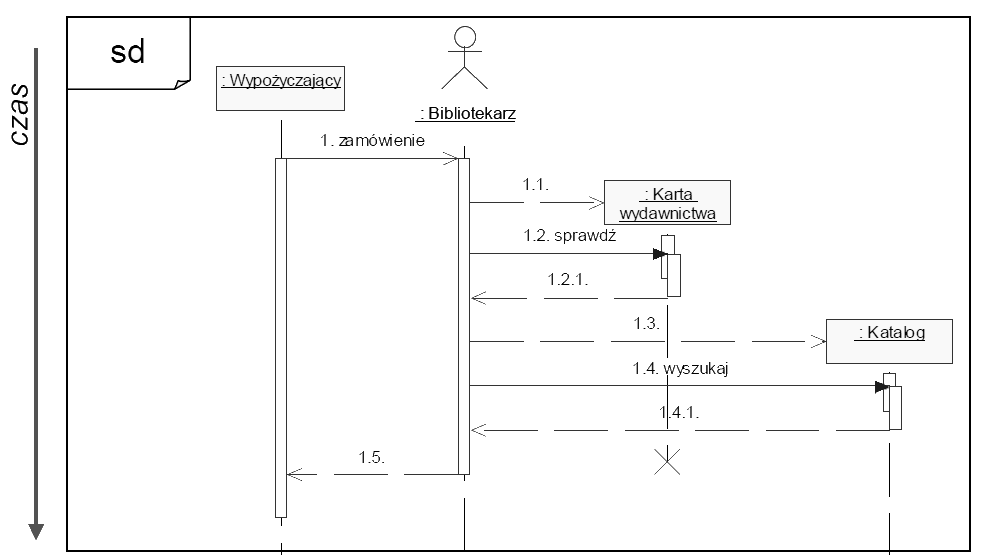
\includegraphics[width=\linewidth]{uml_sek.png}
    \end{figure}

    \subsection{Diagram przypadków użycia.}

    \begin{definition}
        \textbf{Diagram przypadków użycia} służy do przedstawiania:
        \begin{itemize}
            \item interakcji aktora z systemem,
            \item zadań, jakie wykonuje system,
            \item wymagań funkcjonalnych.
        \end{itemize}


        \textbf{Aktorzy} mogą być:
        \begin{itemize}
            \item Ludźmi wchodzącymi w interakcję,
            \item Systemami zewnętrznymi
            \item Częściami systemu, które mają wpływ na funkcjonowanie systemu, ale same przez ten system nie mogą
            być zmieniane (jak np. zegar systemowy).
        \end{itemize}
    \end{definition}

    \begin{figure}[H]
        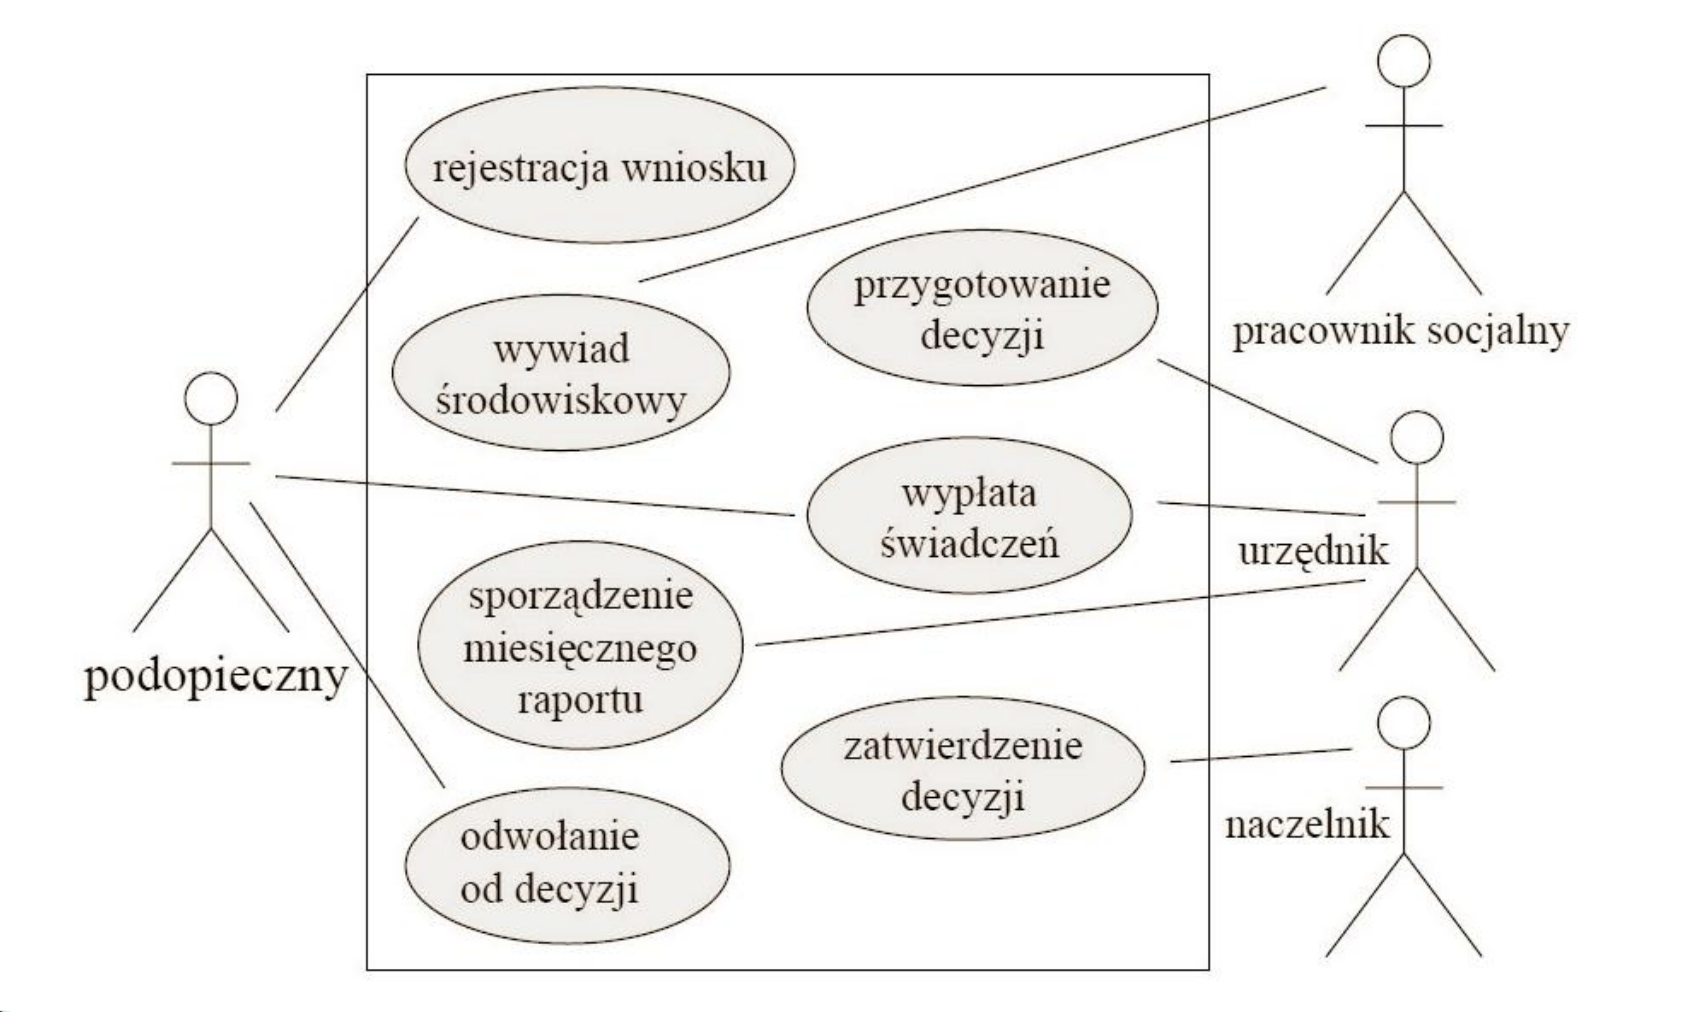
\includegraphics[width=\linewidth]{uml_pu.png}
    \end{figure}

    \newpage

    \section{Klasyfikacja testów.}

    \subsection{Poziomy testów.}
    \begin{definition}
        \textbf{Poziom testów} określa \textbf{sposób} testowania ze względu na \textbf{postać}
        testowanego obiektu w kontekście cyklu życia (\textbf{co testujemy?}).
    \end{definition}

    \subsubsection{Testy jednostkowe.}

    \begin{table}[H]
        \begin{center}
            \begin{tabular}{| p{4cm}| p{12cm}|}
                \hline
                \multicolumn{2}{|c|}{ \textbf{TESTY JEDNOSTKOWE}}\\
                \hline
                \textbf{Podstawa testów} & wymagania na moduły, projekt szczegółowy, kod\\
                \hline
                \textbf{Typowe obiekty} & moduły, programy, funkcje, klasy, procedury\\
                \hline
            \end{tabular}
        \end{center}
    \end{table}


    \begin{itemize}
        \item testowanie modułowe, unit testing
        \item defekty szukane w izolacji od reszty systemu
        \item wykorzystanie zaślepek i sterowników
        \item przeprowadzane przez deweloperów – autorów testowanego kodu
        \item usuwanie defektów bezpośrednio po znalezieniu
        \item brak formalnego procesu zarządzania defektami
    \end{itemize}

    \hfill \\

    \noindent \textbf{TTD} - Test Driven Developement.
    \begin{itemize}
        \item \textbf{Napisanie testu} - sprawdza, że programista rozumie zachowanie nowego kodu.
        \item \textbf{Uruchomienie testu}, który nie przechodzi (testuje uprząż testową i sam test; pokazuje,
        że wystąpi awaria, gdy kod będzie błędny).
        \item \textbf{Napisanie kodu} w minimalnej ilości, wystarczającej do zdania testu; jeśli
        konieczne, dokonanie refaktoryzacji.
    \end{itemize}

    \subsubsection{Testy integracyjne.}

    \begin{table}[H]
        \begin{center}
            \begin{tabular}{| p{4cm}| p{12cm}|}
                \hline
                \multicolumn{2}{|c|}{ \textbf{TESTY INTEGRACYJNE}}\\
                \hline
                \textbf{Podstawa testów} & projekt systemu, architektura, przypadki użycia\\
                \hline
                \textbf{Typowe obiekty} & interfejsy, podsystemy, konfiguracje systemów\\
                \hline
            \end{tabular}
        \end{center}
    \end{table}

    \begin{itemize}
        \item testuje interfejsy i interakcje
        \item im większy zakres integracji, tym trudniej izolować defekty
        \item rozumienie architektury testowanych modułów/systemów
        \item może odbywać się na wielu poziomach (np. integracja systemów)
    \end{itemize}

    \begin{figure}[H]
        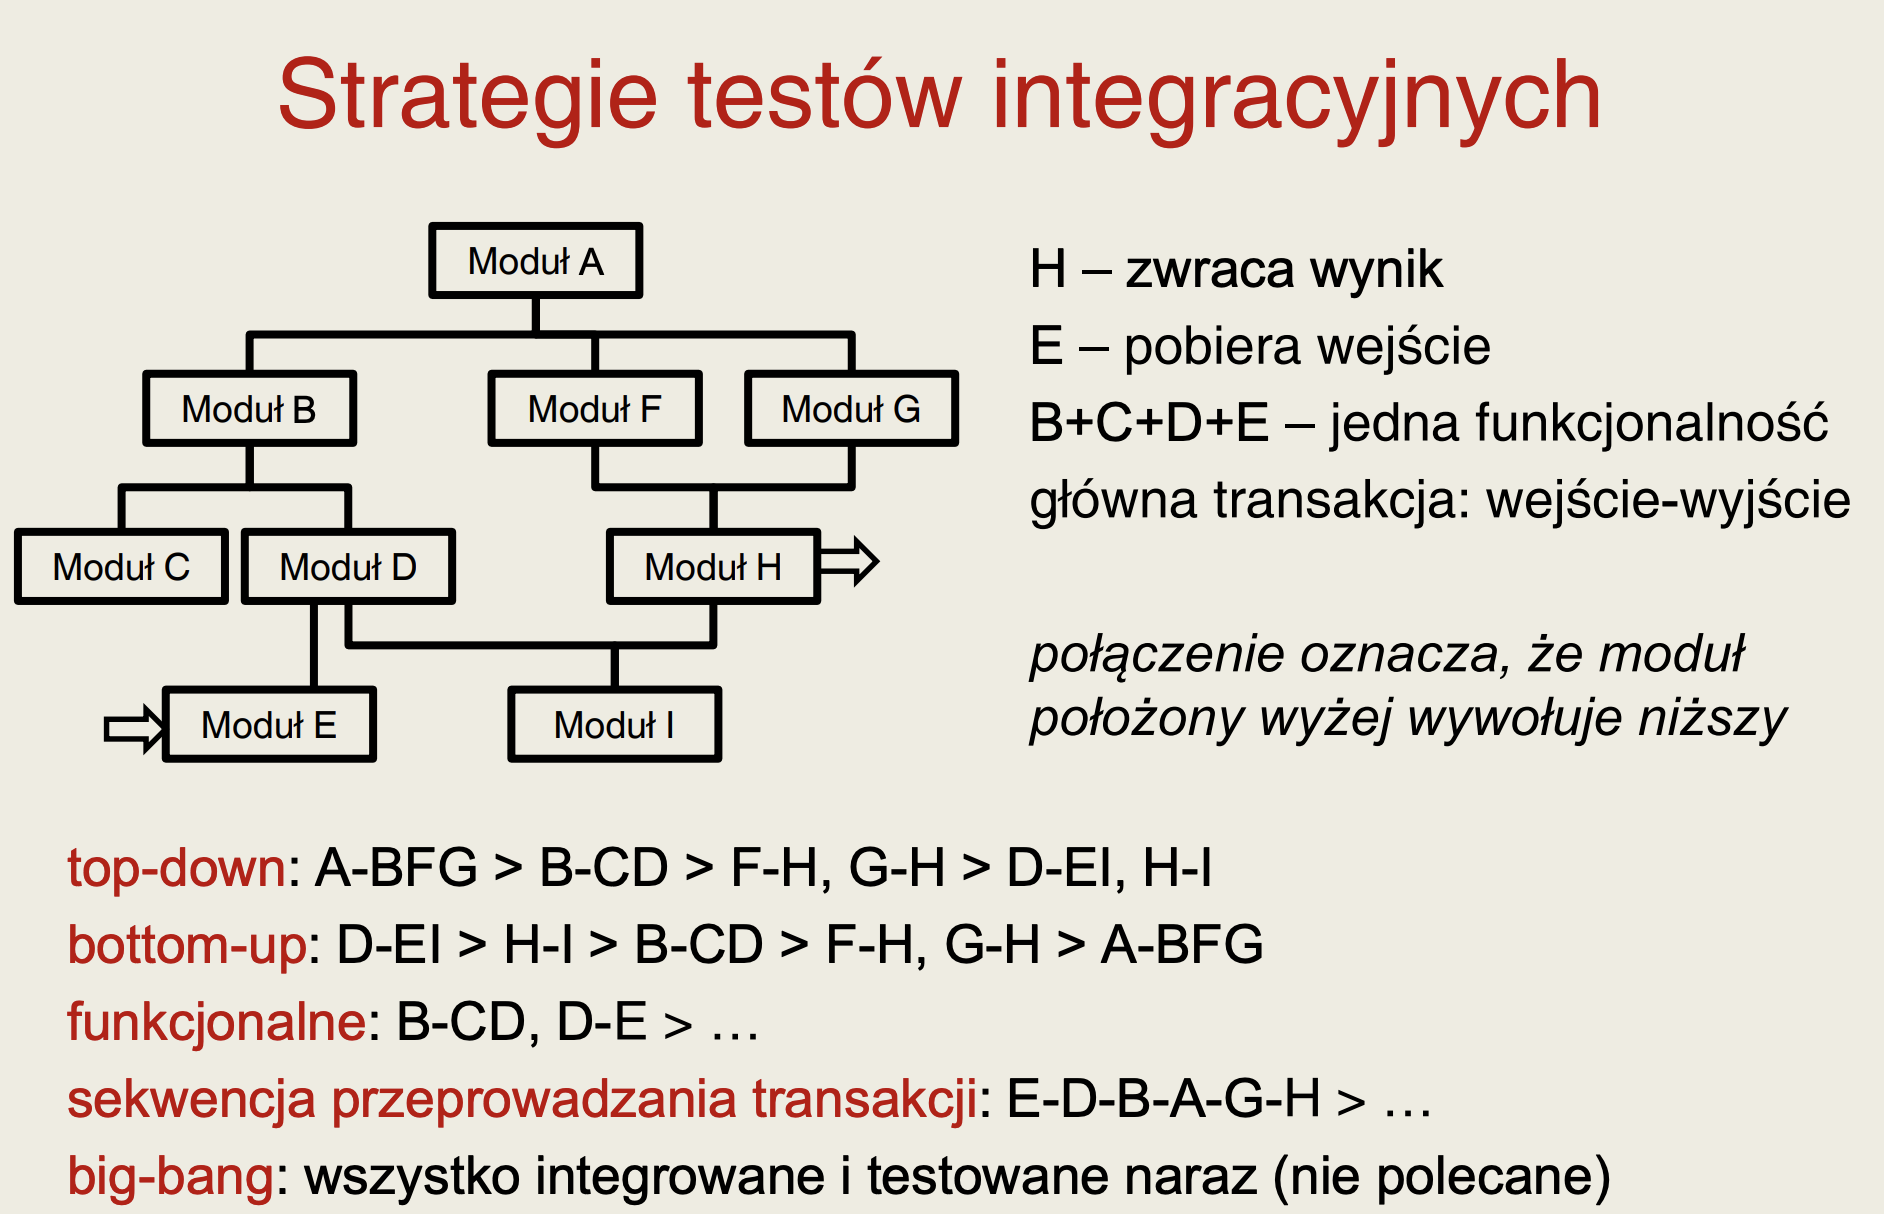
\includegraphics[width=\linewidth]{strat_integr.png}
    \end{figure}

    \subsubsection{Testy systemowe.}

    \begin{table}[H]
        \begin{center}
            \begin{tabular}{| p{4cm}| p{12cm}|}
                \hline
                \multicolumn{2}{|c|}{ \textbf{TESTY SYSTEMOWE}}\\
                \hline
                \textbf{Podstawa testów} & wymagania na system, przypadki użycia,
                specyfikacja funkcjonalna, raporty analizy ryzyka\\
                \hline
                \textbf{Typowe obiekty} & system, podręczniki użytkownika i operatora,
                konfiguracja systemu\\
                \hline
            \end{tabular}
        \end{center}
    \end{table}

    \begin{itemize}
        \item sprawdza zachowanie systemu jako całości
        \item zakres testu określony w planie testów
        \item środowisko testowe podobne do produkcyjnego – minimalizacja ryzyka awarii zależnych od środowiska
        \item często konieczność testowania z niekompletnymi wymaganiami
        \item zwykle przeprowadzane przez niezależny zespół testerski
    \end{itemize}

    \subsubsection{Testy akceptacyjne.}

    \begin{table}[H]
        \begin{center}
            \begin{tabular}{| p{4cm}| p{12cm}|}
                \hline
                \multicolumn{2}{|c|}{ \textbf{TESTY AKCEPTACYJNE}}\\
                \hline
                \textbf{Podstawa testów} & wymagania użytkownika, wymagania na system,
                przypadki użycia, procesy biznesowe, raporty
                analizy ryzyka\\
                \hline
                \textbf{Typowe obiekty} & Procesy biznesowe w pełni zintegrowanego
                systemu, procesy operacyjne i utrzymania systemu,
                procedury, raporty, dane konfiguracyjne\\
                \hline
            \end{tabular}
        \end{center}
    \end{table}

    \begin{itemize}
        \item cel: zyskanie zaufania do systemu
        \item znajdowanie defektów nie jest głównym celem
        \item często przeprowadzane przez klienta lub użytkownika
        \item ocenia gotowość systemu, ale niekoniecznie ostatni etap testów
    \end{itemize}

    \noindent \textbf{Typowe formy testów akceptacyjnych:}
    \begin{itemize}
        \item \textbf{testy akceptacyjne użytkownika (UAT)} – sprawdzenie gotowości do użycia
        \item \textbf{testy operacyjne (OAT)} – akceptacja przez administratora systemu (testy
        backupu, przywracania systemu, zarządzania użytkownikami, utrzymania,
        migracji danych, bezpieczeństwa itp.)
        \item \textbf{testy akceptacyjne wymagane kontraktem/regulacjami}
        \item \textbf{testy alfa, beta (polowe)}
        \begin{itemize}
            \item alfa: przeprowadzane u producenta, ale nie przez zespół deweloperski
            \item beta: przeprowadzane u klienta przez klienta/potencjalnego użytkownika
        \end{itemize}
    \end{itemize}

    \subsection{Typy testów.}

    \begin{definition}
        \textbf{Typ testów} to zbiór czynności testowych właściwych dla weryfikacji systemu
        w oparciu o konkretny powód lub cel testów (\textbf{jak testujemy?}).
    \end{definition}

    \begin{enumerate}
        \item  \textbf{Testowanie funkcjonalne}\\
        Testowanie funkcji wykonywanej przez oprogramowanie - \textbf{co system robi}.

        \item \textbf{Testowanie niefunkcjonalne}\\
        Testowanie niefunkcjonalnej charakterystyki jakościowej (np. niezawodność, wydajność,
        użyteczność) - \textbf{jak system działa}. Wyrażalne ilościowo (np. czas odpowiedzi w testach wydajności).

        \item \textbf{Testowanie strukturalne}\\
        Oparte na strukturze (np. kod, graf przepływu sterowania, struktura menu, model procesu biznesowego).
        Zwykle wykonywane po testach czarnoskrzynkowych, aby sprawdzić stopień przetestowania i wyrazić go ilościowo
        (\textbf{pokrycie}).

        \item \textbf{Retesty i testy regresji}\\
        \textbf{Związane ze zmianą}, tzn. potwierdzenie usunięcia defektów (retesty - testy zmienionych fragmentów kodu)
        oraz poszukiwanie niezamierzonych zmian (regresja - pogarszanie się jakości systemu przy wprowadzaniu zmian;
        testujemy niezmienione fragmenty programu- często automatyzowane).
    \end{enumerate}

    \newpage

    \section{Model Scrum: struktura zespołu, proces wytwarzania oprogramowania, korzyści modelu.}
    \begin{definition}
        \textbf{SCRUM} jest:
        \begin{itemize}
            \item lekki
            \item łatwy do zrozumienia
            \item bardzo trudny do opanowania
        \end{itemize}

        Teoria SCRUMa opiera się na trzech filarach:
        \begin{itemize}
            \item \textbf{Przejżystość} - wszystkie istotne aspekty procesu muszą być widoczne dla osób odpowiedzialnych za osiągane rezultaty
            \item \textbf{Adaptacja} - powinna być ciągła. Korekta musi być wykonana jak najszybciej, by ograniczyć dalsze następstwa problemów
            \item \textbf{Inspekcja} - poddawane regularnej inspekcji są zarówno scrumowe artefakty jak i postępy prac
        \end{itemize}
    \end{definition}

    \subsection{Struktura zespołu}

    \begin{definition}
        \textbf{Struktura zespołu} \\
        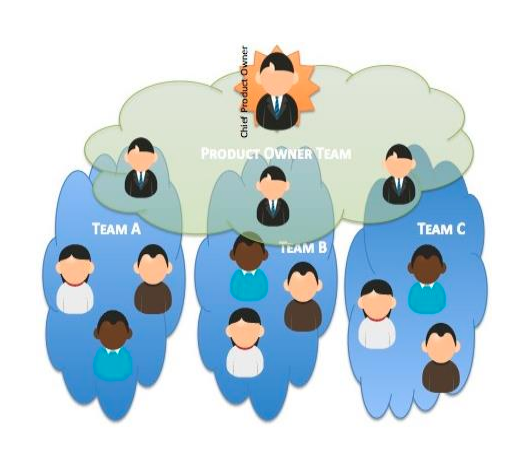
\includegraphics[width=\linewidth]{scrum_teams.png}
    \end{definition}

    \begin{definition}
        \textbf{Product owner} - jest odpowiedzialny za maksymalizację wartości produktu i pracy Zespołu Deweloperskiego. jest jedyną osobą zarządzającą Rejestrem Produktu (Product Backlog) co rozumiemy przez:
        \begin{itemize}
            \item Jasne artykułowanie elementów Rejestru Produktu i określanie ich kolejności w sposób zapewniający osiąganie założonych celów i misji
            \item Zapewnianie, że Rejestr Produktu jest dostępny, przejrzysty oraz jasny dla wszystkich i, że dobrze opisuje to, czym Zespół Scrumowy będzie się zajmował
        \end{itemize}
    \end{definition}

    \begin{definition}
        \textbf{Zespół Deweloperski}:
        \begin{itemize}
            \item Jest złożony z profesjonalistów
            \item Ma za zadanie dostarczenie (na zakończenie każdego Sprintu), gotowego do wydania Przyrostu produktu
            \item Zalecana liczebność: 3-9 osób
            \item Są samoorganizujące się
            \item Jest wielofunkcyjny, w swoim składzie posiadają wszystkie umiejętności niezbędne do wytworzenia Przyrostu
            \item Scrum nie przewiduje tytułów innych niż ``Deweloper'' dla członków Zespołu Deweloperskiego
            \item Odpowiedzialność za wykonywaną pracę ponosi cały Zespół Deweloperski; nie składają się z podzespołów
        \end{itemize}
    \end{definition}

    \begin{definition}
        \textbf{Scrum Master} - jest odpowiedzialny za to, by Scrum był rozumiany i stosowany. Scrum Masterzy dokonują tego poprzez upewnianie się,
        że Zespół Scrumowy stosuje się do założeń teorii Scruma, jego praktyk i reguł postępowania. Scrum Master wspiera zarówno Właściciela Produktu jak i zespól deweloperski.
    \end{definition}

    \subsection{Zdarzenia}

    \begin{definition}
        \textbf{Zdarzenia} \\
        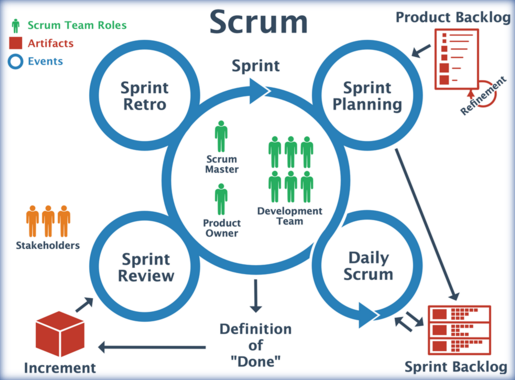
\includegraphics[width=\linewidth]{scrum_events.png}
    \end{definition}

    \begin{definition}
        \textbf{Planowanie sprintu} - planowanie co zostanie wykonane podczas najbliższego sprintu:
        \begin{itemize}
            \item Jest ograniczone czasowo (8h dla miesięcznego sprintu i proporcjonalnie)
            \item Planowanie Sprintu składa się z dwóch części:
            \begin{itemize}
                \item Co zostanie dostarczone
                \item Jaka praca zostanie wykonana
            \end{itemize}
        \end{itemize}
    \end{definition}

    \begin{definition}
        \textbf{Sprint} - serce SCUMa:
        \begin{itemize}
            \item Ograniczony czasowo - trwa miesiąc lub krócej
            \item Podczas Sprintu wytwarzany jest Przyrost „Ukończonej”, używalnej i potencjalnie gotowej do wydania funkcjonalności
            \item Ma stałą długość przez cały okres trwania prac
            \item Niedozwolone są zmiany, które wpłyną na cel Sprintu
            \item Skład Zespołu Deweloperskiego i jego cel jakościowy pozostają niezmienne
            \item Przerwanie sprintu:
            \begin{itemize}
                \item Tylko product owner ma prawo przerwać sprint
                \item Sprint może zostać przerwany, jeśli cel Sprintu się zdezaktualizuje
                \item Powinien zostać przerwany, jeśli kontynuowanie prac nie ma sensu w zaistniałych okolicznościach
                \item Przerwania Sprintów zużywają zasoby, ponieważ wszyscy muszą się przegrupować podczas kolejnego Planowania Sprintu, aby móc rozpocząć nowy
            \end{itemize}
        \end{itemize}
    \end{definition}

    \begin{definition}
        \textbf{Daily scrum} - jest spotkaniem ograniczonym czasowo do 15 minut, w którym każdy z członków zespołu wyjaśnia:
        \begin{itemize}
            \item Co zostało wykonane od ostatniego potkania
            \item Co zostanie wykonane przed kolejnym spotkaniem
            \item Jakie przeszkody stoją na drodze
        \end{itemize}
    \end{definition}

    \begin{definition}
        \textbf{Przegląd sprintu} - organizowany jest na zakończenie Sprintu w celu przeprowadzenia inspekcji Przyrostu i dostosowaniu, jeśli zajdzie taka potrzeba, Rejestru Produktu. \\
        Podczas Przeglądu Sprintu \textbf{Zespół Scrumowy} i \textbf{interesariusze} wspólnie omawiają to, co zostało ukończone w Sprincie. \\
        Może trwać maksymalnie 4h dla miesięcznego Sprintu.
    \end{definition}

    \begin{definition}
        \textbf{Retrospektywa Sprintu} - jest okazją dla zespołu Scrumowego do przeprowadzenia inspekcji swoich działań i opracowania planu usprawnień. Ma na celu:
        \begin{itemize}
            \item Sprawdzenie, co działo się w ostatnim Sprincie, biorąc pod uwagę ludzi, zależności, procesy i narzędzia
            \item Zidentyfikowanie i uporządkowanie istotnych elementów, które sprawdziły się w działaniu oraz tych, które kwalifikują się do poprawy
            \item Stworzenie planu wprowadzania w życie usprawnień sposobu wykonywania pracy przez Zespół Scrumowy
        \end{itemize}
    \end{definition}

    \subsection{Artefakty}

    \begin{definition}
        \textbf{Rejestr produktu} - uporządkowana lista tego co może byc potrzebne w produkcie. Jest to jedyne źródło wymaganych zmian, które mają zostać wprowadzone.
        Odpowiedzialny z rejestr produktu jest Product owner.
    \end{definition}

    \begin{definition}
        \textbf{Rejestr sprintu} - podzbiór elementów Rejestru produktu. Jest to lista rzeczy do wykonania w danyc sprincie rozszeżona dodatkowo o plan ich wykonania.
        Rejestr Sprintu definiuje pracę, jaką Zespół Deweloperski wykona by przekształcić elementy Rejestru Produktu w „Ukończony” Przyrost. \\
        Rejestr Sprintu należy tylko i wyłącznie do Zespołu Deweloperskiego.
    \end{definition}

    \begin{definition}
        \textbf{Przyrost} - suma wszystkich elementów Rejestru Produktu zakończonych podczas Sprintu i wszystkich Sprintów poprzednich. \\
        Na koniec Sprintu nowy Przyrost musi być ``Ukończony''.
    \end{definition}

    \newpage




    \section{Wymagania w projekcie informatycznym: klasyfikacja, źródła, specyfikacja, analiza.}

    \begin{definition}
        \textbf{Wymagania} - opis funkcji (usług), które mają być realizowane przez system i opis ograniczeń dla systemu. \\
        Wymagania nie opisują jak system ma działać a co ma wykonywać.
    \end{definition}

    \subsection{Klasyfikacja}

    \begin{definition}
        Wymagania dzielimy na:
        \begin{itemize}
            \item \textbf{Funkcjonalne} - opisują jakie funkcje powinien mieć system, np. ``wprowadzanie nowej faktury'' lub ``generowanie raportu miesięcznego''
            \item \textbf{Pozafunkcjonalne} - opisują najczęściej pewne własności danych funkcjonalności, np. ``minimum 20 faktur na godzinę'', ``średni czas między awariami 2000000h'', itp.
        \end{itemize}
    \end{definition}

    \begin{definition}
        \textbf{Klasyfikacja atrybutów jakości oprogramowania}
        \begin{itemize}
            \item \textbf{F}unctionality - funkcjonalność
            \item \textbf{U}sability – użyteczność
            \item \textbf{R}eliability – niezawodność
            \item \textbf{P}erformance – wydajność
            \item \textbf{S}ecurity - bezpieczeństwo
        \end{itemize}
        w skrócie \textbf{FURPS}
    \end{definition}

    \subsection{Źródła}

    \begin{definition}
        \textbf{System powinien…} \\
        Jest to sposób spisywania wymagań w stylu: ``System powinien umożliwić wystawianie faktur'', ``System powinien generować zestawienie miesięczne faktur'', ``Faktura powinna zawierać co najmniej jedną pozycję''. \\

        Zalety:
        \begin{itemize}
            \item Łatwość spisywania
        \end{itemize}

        Wady:
        \begin{itemize}
            \item Słaba czytelność
            \item Trudne sprawdzanie kompletności, spójności
        \end{itemize}

        Obecnie nie używany
    \end{definition}


    \begin{definition}
        \textbf{Funkcje systemu} \\
        Polega na opisywaniu poszczególnych funkcji systemu. Analogicznie do funkcji matematycznych, każda funkcja systemu informatycznego ma swoje wejście, wyjście, efekty uboczne. \\
        Przykładowo, rozpatrując funkcję wystawiania faktury, wejściem mogą być pozycje faktury, wyjściem wydruk faktury (lub wysłanie jej faksem), natomiast efektem ubocznym zapisanie tej faktury w rejestrze faktur. \\

        Wady:
        \begin{itemize}
            \item Słaba czytelność
            \item Trudne do zrozumienia
        \end{itemize}

        Obecnie nie używany
    \end{definition}


    \begin{definition}
        \textbf{Przypadki użycia} \\
        Przykład: \\

        \textbf{UC1: Wystawianie faktury} \\
        \textbf{Atrybuty:} \\
        \textbf{Główny aktor: Użytkownik} \\
        \textbf{Priorytet: Wysoki} \\
        \textbf{Źródło: Łukasz Olek} \\

        \textbf{Główny scenariusz:} \\
        1. Sprzedawca pragnie wystawić fakturę. \\
        2. Sprzedawca wpisuje pozycje faktury. \\
        3. System podlicza fakturę, nadaje jej nowy numer i zapisuje w rejestrze. \\
        4. Sprzedawca drukuje fakturę. \\
        \textbf{Rozszerzenia:} \\
        3.A. Sprzedawca nie dodał żadnej pozycji \\
        3.A.1. System prosi o ponowne wprowadzenie pozycji (powrót do 2.) \\

        Zalety:
        \begin{itemize}
            \item Łatwość spisywania
            \item Czytelność
            \item Łatwość zrozumienia i wyobrażenia sobie przyszłego systemu
        \end{itemize}

    Jako mapę łączącą pojedyncze przypadki użycia można potraktować diagram przypadków użycia (UML).
    \end{definition}
    
    
    \begin{definition}
    \textbf{Historyjki użytkownika} \\
    
    \textbf{Who? What? Why?} \\
    
    Wzór: \\
    
    \textbf{jako} - osoba, przypisana rola \\
    \textbf{chcę} - cacha, funkcjonalność, czynność \\
    \textbf{ponieważ} - uzasadnienie, rezultat, korzyść \\
    \end{definition}
    
    \subsection{Analiza}
    
    \begin{definition}
    Celem analizy wymagań jest stworzenie modelu systemu, zwanego modelem analitycznym. Wysiłek uczestników projektu skupia się na strukturalizowaniu i formalizowaniu zabranych wcześniej wymagań. \\
    Inaczej mówiąc po przeanalizowaniu przez nas zebranych wymagań musimy to przełożyć na diagramy UML.
    \end{definition}
    
    \begin{definition}
    \textbf{Model analityczny} - reprezentuje tworzony system z perspektywy użytkownika; opis co system powinien robić
    \end{definition}
    
    \begin{definition}
    \textbf{Analityczny model obiektowy} (diagramy klas) - odzwierciedla indywidualne koncepcje korzystania z systemu, ich właściwości i relacje między nimi
    \end{definition}
    
    \begin{definition}
    \textbf{Model dynamiczny} (diagramy sekwencji i stanów) - koncentruje się na zachowaniu systemu
    \end{definition}
    
   \newpage

    \section{Analiza obiektowa: modele obiektowe i dynamiczne, obiekty encjowe, brzegowe i sterujące.}

        \subsection{Diagram klas}
            
            Diagram klas ma za zadanie:
            \begin{itemize}
                \item przedstawić strukturę systemu w modelach obiektowych poprzez
                    ilustrację struktury klas i zależności między nimi
                \item przedstawić podział odpowiedzialności pomiędzy klasy systemu
                    i rodzaj wymienianych pomiędzy nimi komunikatów
            \end{itemize}

            \begin{center}
                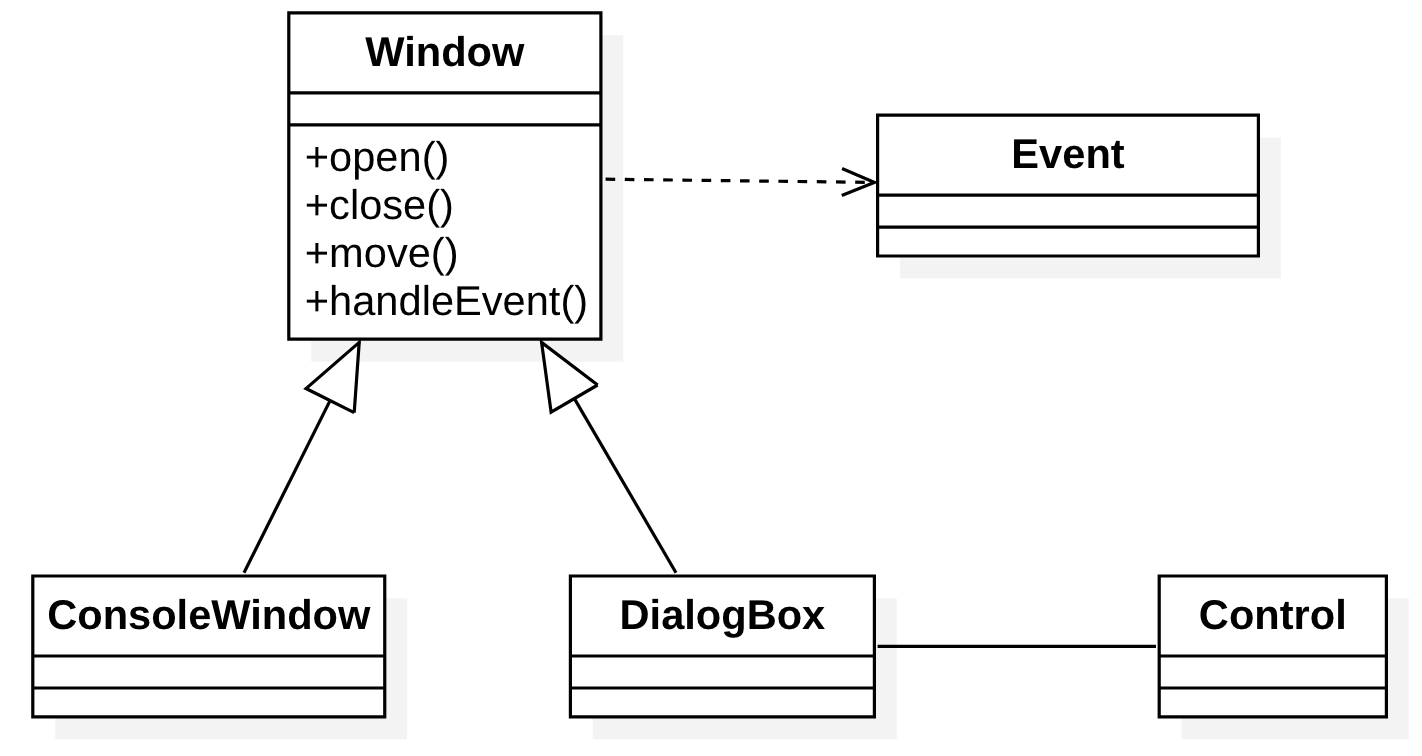
\includegraphics[scale=0.40]{ooad/uml.png}
            \end{center}


            \subsubsection{Klasy}
                
                Podstawowa część diagramu klas. Służą m.in. do opanowania słownictwa
                tworzonego systemu.

                Klasa składa się z:
                \begin{enumerate}
                    \item Nazwy
                    \item Atrybutów - czyli nazwanych właściwości klasy
                    \item Operacji - implementacji pewnej usługi, której można żądać
                        od obiektów klasy
                    \item Odpowiedzialności (opcjonalnie)
                \end{enumerate}

                \begin{center}
                    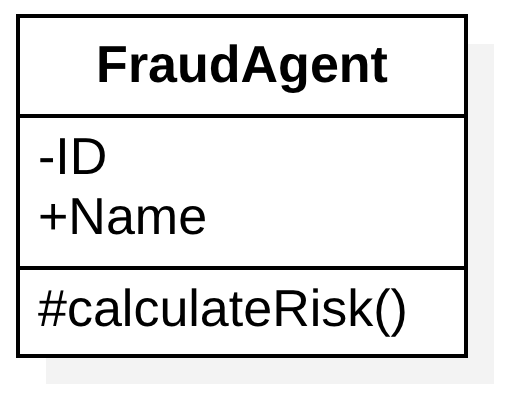
\includegraphics[scale=0.40]{ooad/class.png}
                \end{center}
                    
            \subsubsection{Widoczność pól}

                \begin{itemize}
                    \item \textbf{+} public
                    \item \textbf{-} private
                    \item \textbf{\#} protected
                    \item \textbf{\~} package 
                \end{itemize}

            \subsubsection{Związki}

                \begin{itemize}
                    \item Asocjacja

                        \begin{center}
                            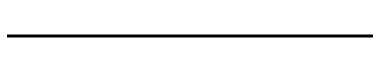
\includegraphics[scale=0.40]{ooad/association.png}
                        \end{center}
                    
                    \item Zależność
                        
                        Informuje nas, że klasa używa innej klasy. Przykład:
                        EventHandler i Event.
                        \begin{center}
                            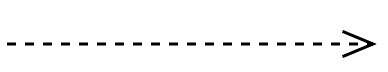
\includegraphics[scale=0.40]{ooad/dependency.png}
                        \end{center}
                    
                    \item Generalizacja

                        Czyli dziedziczenie lub uogólnienie. Określa zależność 
                        między klasą pochodną a klasą bazową.
                        \begin{center}
                            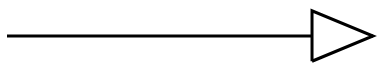
\includegraphics[scale=0.40]{ooad/generalization.png}
                        \end{center}
                    
                    \item Realizacja

                        Określa zależność między implementacją a interfejsem.
                        Przyład: ArrayList i List.

                        \begin{center}
                            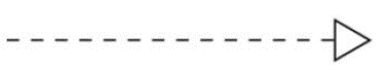
\includegraphics[scale=0.40]{ooad/realization.png}
                        \end{center}
                    
                    \item Agregacja

                        Określa zależność między częścią a całością.
                        Przykład: cegła i mur.

                        \begin{center}
                            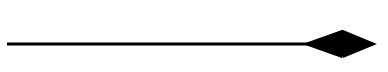
\includegraphics[scale=0.40]{ooad/composition.png}
                        \end{center}
                    
                    \item Kompozycja

                        Zwana również silną agregacją. Tak jak agregacja, określa
                        zależność między częścią a całością, jednak część nie może 
                        istnieć bez całości. Przykład: wydział i uczelnia.

                        \begin{center}
                            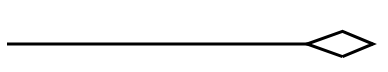
\includegraphics[scale=0.40]{ooad/aggregation.png}
                        \end{center}
                \end{itemize}

        \newpage
        \subsection{Modele dynamiczne}
            
            \subsubsection{Diagram stanów}

                W UML dynamiczne aspekty systemu modeluje się za pomocą maszyny stanów.
                Diagram stanów zapewnia graficzną reprezentację stanów, przejść, zdarzeń i akcji.
                Notacja ta pozwala zwizualizować zachowanie obiektu w sposób, który pozwala
                podkreślić ważne elementy życia tego obiektu.

                    \begin{center}
                        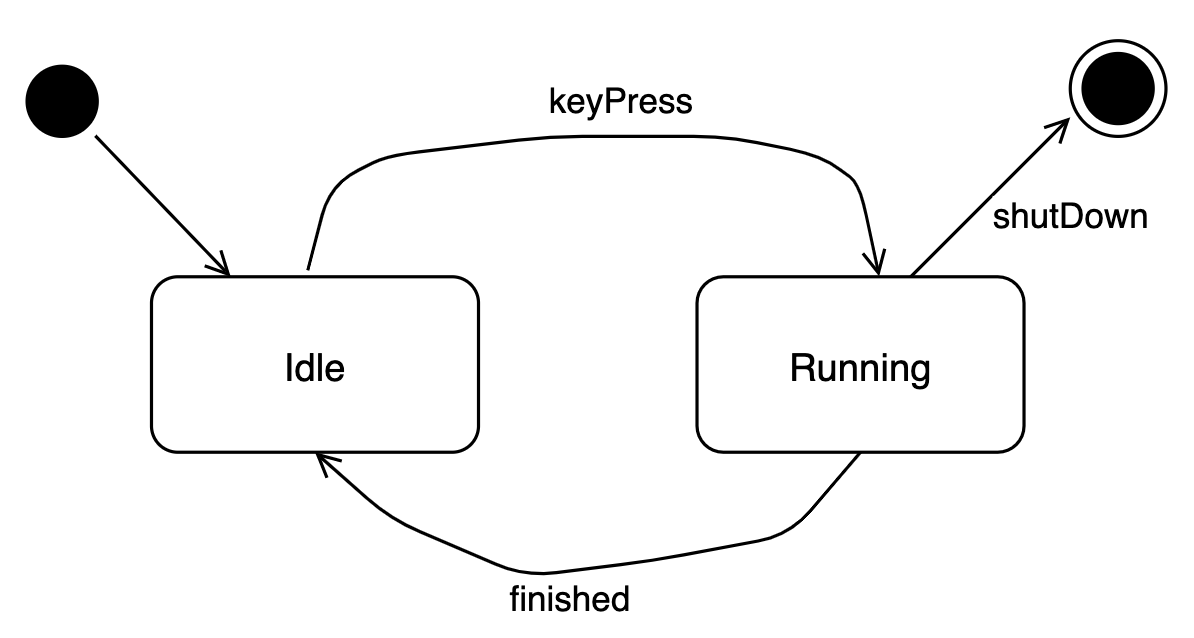
\includegraphics[scale=0.40]{state-diagram/diagram.png}
                    \end{center}


                \begin{itemize}
                    \item \textbf{Stan}

                        Stan na diagramie reprezentuje sytuację lub stan obiektu,
                        w którym spełnia on pewien warunek, wykonuje jakąś czynność lub czeka
                        na jakieś zdarzenie. Obiekt pozostaje w stanie przez określony czas.
                        Graficznie stan renedeorwany jest jako 
                        prostokąt z zaokrąglonymi narożnikami.

                        \begin{center}
                            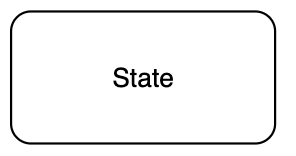
\includegraphics[scale=0.60]{state-diagram/state.png}
                        \end{center}

                        \begin{itemize}
                            \item Podstany

                                Możliwe jest podzielenie stanu na wewnętrzne podstany,
                                z wewnętrznymi przejściami, akcjami, itp.

                            \begin{center}
                                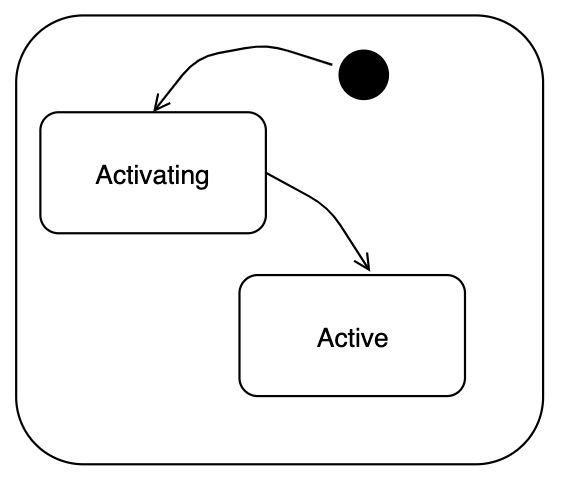
\includegraphics[scale=0.50]{state-diagram/substate.png}
                            \end{center}

                            \item Stan początkowy

                                Wskazuje domyślne miejsce początkowe dla danego stanu lub automatu.
                                Stan początkowy jest reprezentowany jako wypełnione czarne kółko.
                            \begin{center}
                                
\includegraphics[scale=0.60]{state-diagram/begin.png}
                            \end{center}

                            \item Stan końcowy

                                Wskazuje, że wykonanie automatu stanów lub danego stanu zostało
                                zakończone. Stan końcowy jest reprezentowany jako wypełnione 
                                czarne koło otoczone niewypełnionym okręgiem.

                            \begin{center}
                                
\includegraphics[scale=0.60]{state-diagram/end.png}
                            \end{center}

                        \end{itemize}
                        
                    \item \textbf{Przejścia}
                            
                            
                            Przejście to związek między dwoma stanami wskazujący, że obiekt
                            w pierwszym stanie wykona określone działania i przejdzie w drugi
                            stan, gdy wystąpi określone zdarzenie i spełnione zostaną
                            określone warunki.

                        \begin{itemize}
                            \item Zdarzenia

                                Wystąpienie bodźca, który może wywołać zmianę stanu.

                            \begin{center}
                                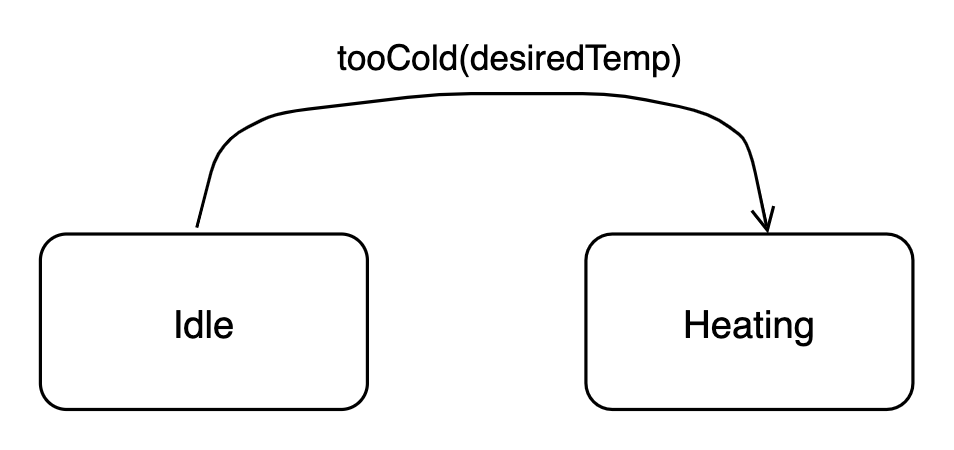
\includegraphics[scale=0.50]{state-diagram/event.png}
                            \end{center}


                            \item Akcje

                                Wykonywalne obliczenie atomowe. Akcje mogą obejmować wywołania 
                                operacji (do obiektu będącego właścicielem maszyny stanu, a także
                                do innych widocznych obiektów), utworzenie lub zniszczenie innego
                                obiektu lub wysłanie sygnału do obiektu. Istnieje specjalny zapis
                                do wysyłania sygnału - nazwa sygnału jest poprzedzona słowem 
                                kluczowym send jako wskazówką wizualną.

                        \begin{center}
                            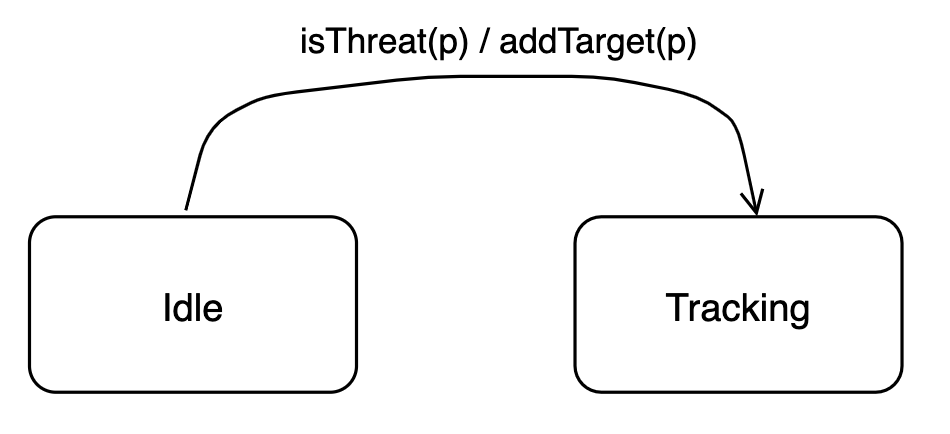
\includegraphics[scale=0.50]{state-diagram/action.png}
                        \end{center}

                        \begin{center}
                            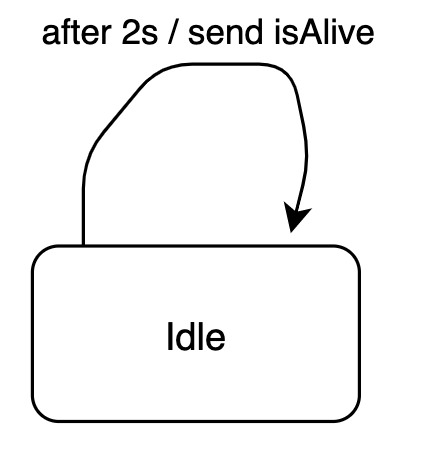
\includegraphics[scale=0.50]{state-diagram/signal.png}
                        \end{center}

                        \end{itemize}
                \end{itemize}

            \subsubsection{Diagram sekwencji}

                Diagram ten opisuje interakcje pomiędzy częściami systemu w postaci sekwencji 
                komunikatów wymienianych między nimi. Ukazuje dynamiczne aspekty realizacji 
                scenariuszy, w których dochodzi do złożonych oddziaływań pomiędzy obiektami 

                \begin{center}
                    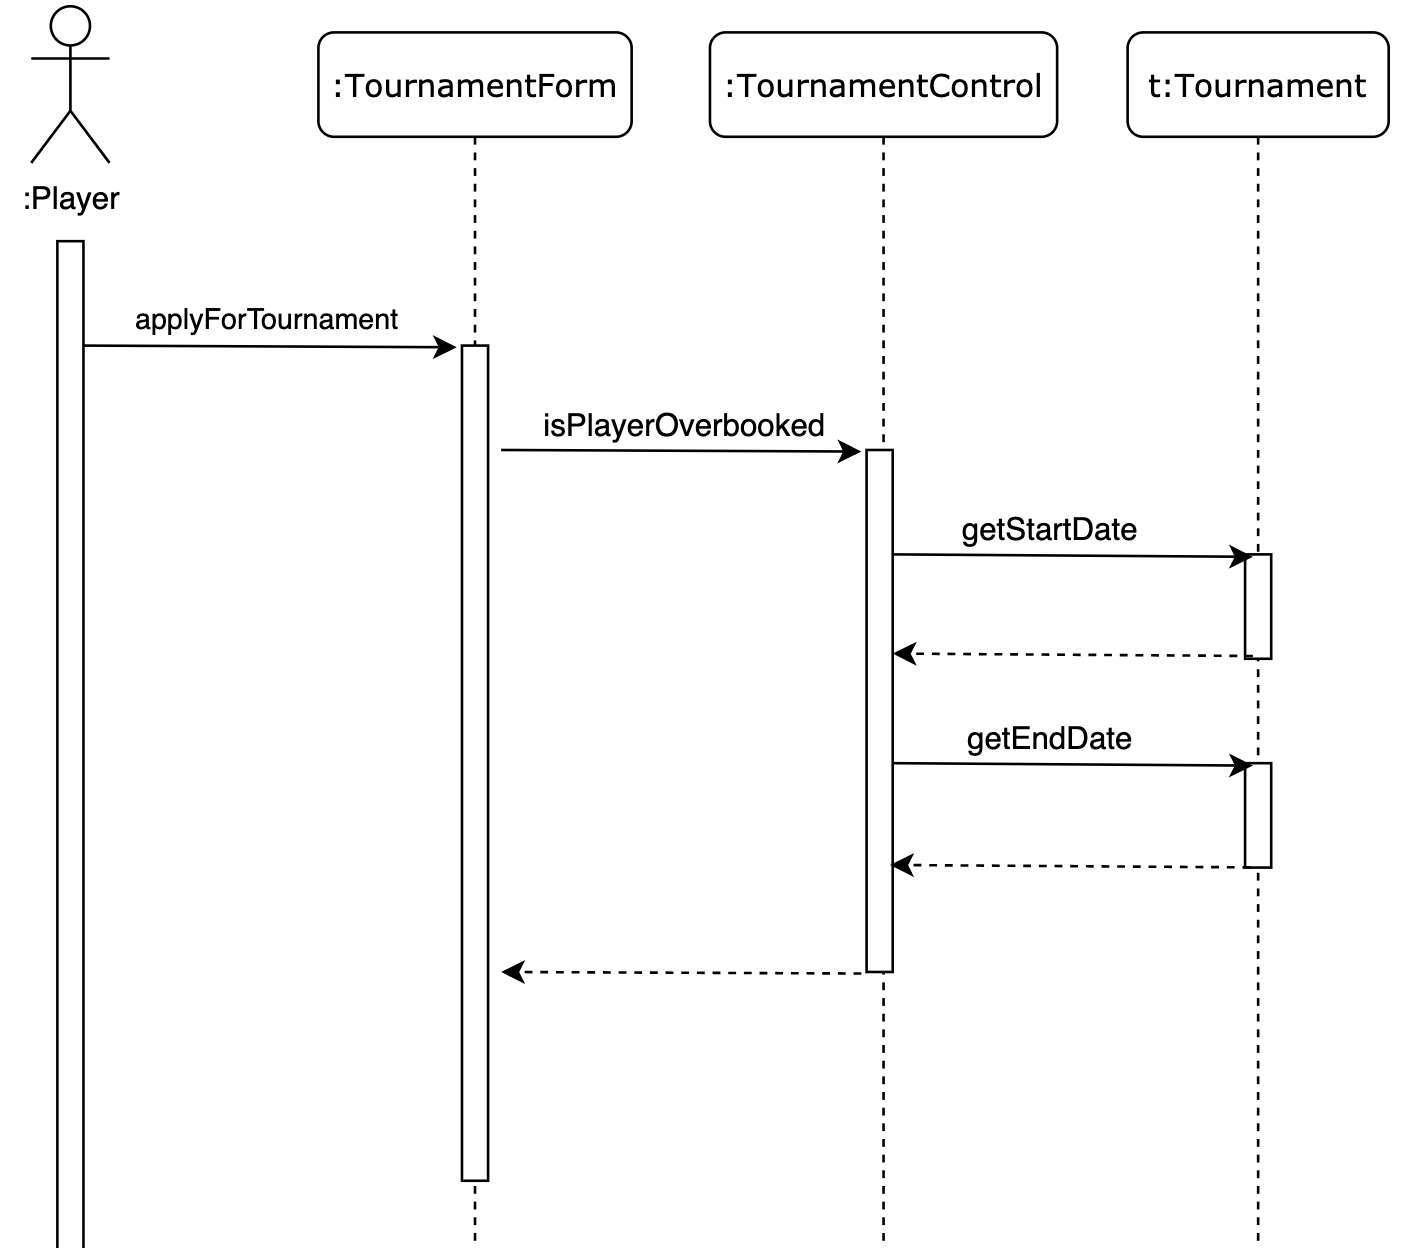
\includegraphics[scale=0.40]{ooad/sequence.png}
                \end{center}

                Rodzaje komunikatów:

                \begin{itemize}
                    \item Wywołanie funkcji
                        
                        \begin{center}
                            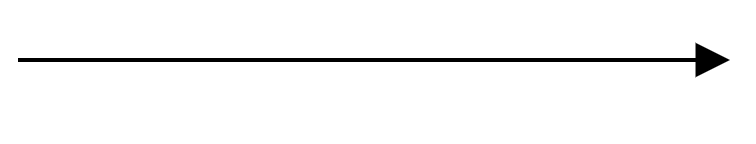
\includegraphics[scale=0.35]{ooad/normal.png}
                        \end{center}

                    \item Powrót z wywołania
                        
                        \begin{center}
                            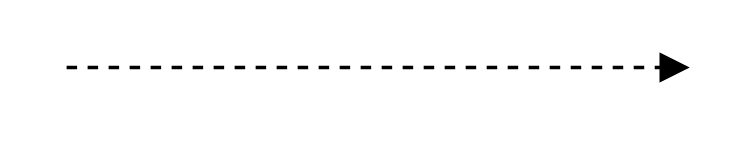
\includegraphics[scale=0.40]{ooad/return.png}
                        \end{center}

                    \item Wywołanie asynchoniczne
                        
                        \begin{center}
                            \includegraphics[scale=0.40]{ooad/async.png}
                        \end{center}

                \end{itemize}

        \subsection{Encja-Brzeg-Sterowanie}

            Model ten dzieli obiekty wchodzące w ramy systemu na trzy typy:
            \begin{itemize}
                \item \textbf{Obiekty encji}

                    Reprezentują trwałą informację przetwarzaną przez system

                \item \textbf{Obiekty brzegowe}

                    Odzwierciedlają interakcje między aktorami a systemem

                \item \textbf{Obiekty sterujące}
            
                    Odpowiadają za realizację przypadków użycia        

            \end{itemize}

            \begin{center}
                \includegraphics[scale=0.40]{ooad/ecb.png}
            \end{center}

            \begin{center}
                \includegraphics[scale=0.50]{ooad/ecb-uml.png}
            \end{center}
   \newpage
   
   \section{Wzorce architektury systemów.}

        \subsection{Architektura warstwowa}

        Efektem dekompozycji hierarchicznej jest
        uporządkowany zbiór warstw. Warstwa stanowi
        zgrupowanie podsystemów oferujących
        powiązane usługi.

        Wyróżniamy dwa rodzaje architektury warstwowej:
        otwartą i zamkniętą.

        Zalety:
        \begin{itemize}
            \item modyfikowalność
            \item prostota wykorzystania warstwy
            \item spójność i przejrzystość
            \item wielokrotne wykorzystanie
            \item naturalna ewolucja z tradycyjnego modelu aplikacji
        \end{itemize}
        
            \subsubsection{Architektura otwarta}
            
            W otwartej architekturze warstwowej warstwa może wywołać
            dowolną z warstw poniżej niej.

            \begin{center}
                \includegraphics[scale=0.30]{patterns/swing.png}
            \end{center}

            Przykłady:
            \begin{itemize}
                \item Serverless
                \item Swing
            \end{itemize}

            \subsubsection{Architektura zamknięta}

            W zamkniętej architekturze warstwa może wywołać tylko wartstwę
            bezpośrednio pod nią

            \begin{center}
                \includegraphics[scale=0.30]{patterns/tcp.png}
            \end{center}

            Przykłady:
            \begin{itemize}
                \item ISO/OSI
                \item TCP/IP
            \end{itemize}

            \subsubsection{Architektura trójwarstwowa}

            Architektura trójwarstwowa to architektura typu klient-serwer,
            często stosowana przy tworzeniu aplikacji internetowych.

            Warstwy:
            \begin{enumerate}
                \item Wartwa prezentacji

                    Interfejs użytkownika. Tłumaczy żądania i wyniki
                    do i z języka zrozumiałego dla użytkownika.

                \item Warstwa logiki biznesowej

                    Koordynuje pracę aplikacji, przeytwarza żądania
                    wartstwy prezentacji, dokonuje obliczeń.

                \item Warstwa danych

                    Zawiera w sobie mechanizmy persystencji danych
                    (jak na przykład bazy danych) oraz dostępu do nich.
            \end{enumerate}
        
            \begin{center}
                \includegraphics[scale=0.30]{patterns/three-layer.png}
            \end{center}

        \subsection{Model View Controller}

            Wzorzec architektoniczny, dzielący system na trzy główne części:
            \begin{enumerate}
                \item \textbf{Model}
                    
                    Reprezentuje podstawową część funkcjonalności systemu

                \item \textbf{Widok}

                    Wyświetla dane dostarczone przez model użytkownikowi

                \item \textbf{Kontroler}
                    
                    Przyjmuje dane wejściowe od użytkownika oraz przetwarza jego żądania

            \end{enumerate}

            \begin{center}
                \includegraphics[scale=0.30]{patterns/mvc.png}
            \end{center}

            Przykłady:
            \begin{itemize}
                \item Smalltalk
                \item Swing
            \end{itemize}

        \subsection{Pipeline (filtry i potoki)}

            Wzorzec Pipeline pozwala na uporządkowanie systemu, która przetwarza
            strumienie danych. Każdy krok przetwarzania jest zamknięty w filtrze
            Dane przesułane są pomiędzy elementami za pomocą potoków (pipes).

            \begin{center}
                \includegraphics[scale=0.30]{patterns/pipeline.png}
            \end{center}

            Przykłady:
            \begin{itemize}
                \item Unix pipeline
                \item Multimedia (GStreamer, Membrane)
            \end{itemize}

        \subsection{Client - Server}

            Architektura ta polega na podziale systemu na dostawcę usług (server)
            oraz ich odbiorców (clients). Serwer oczekuje na żądania (request) klientów,
            przetwarza je, a następnie wysyła odpowiedzi (response). Pracuje zatem, w 
            przeciwieństwie do klientów, w trybie pasywnym.
            
            \begin{center}
                \includegraphics[scale=0.30]{patterns/client-server.png}
            \end{center}

            Przykłady:
            \begin{itemize}
                \item Serwer WWW i przeglądarka internetowa
                \item System bankowy
            \end{itemize}

        \newpage
        \subsection{Peer-to-Peer}
            
            Każdy z podsytemów (hostów, peerów) może pełnić zarówno funkcję 
            serwera, jak i klienta. Architektura systemu jest rozproszona, każdy
            z hostów ma te same uprawnienia.

            \begin{center}
                \includegraphics[scale=0.30]{patterns/peer2peer.png}
            \end{center}

            Przykłady:
            \begin{itemize}
                \item Torrenty
                \item Videochaty (nie zawsze)
            \end{itemize}

    \newpage

    {\Large Inżynieria systemów}

    \section{Relacyjny model danych, normalizacja relacji (w szczególności algorytm doprowadzenia relacji do postaci Boyce’a-Codda), przykłady.}
    
    LINK :\\
    \url{http://www.informatyka.orawskie.pl/?pl_relacyjny-model-bazy-danych,112}
    \url{https://drive.google.com/drive/folders/1vsBsmaooGSXhDF0WGDRy8CElA7667xy9}
    
    \subsection{Relacyjny model danych}
    
    W systemach baz danych opartych o model relacyjny zachodzą własności
    \begin{itemize}
        \item Dane przechowywane są w strukturach nazywanych \textbf{tabelami}. Tabelę można traktować jako strukturę reprezentującą (i przedstawiającą) tzw. relację bazodanową
        \item Wiersz tabeli zawiera dane reprezentujące pewien \textbf{byt} (obiekt, czynność, zdarzenie, zjawisko) lub \textbf{zależność między bytami} (związek)
        \item Cechy „bytu”, zwane \textbf{atrybutami} są reprezentowane w \textbf{kolumnach}. Kolumny mają \textbf{nazwę} i określony \textbf{typ} danych związany z dziedziną atrybutu. Dane wpisywane do kolumny są elementami dziedziny i są logicznie niepodzielne (elementarne, atomowe)
        \item Każdy wiersz w tabeli musi (powinien) być \textbf{unikalny}
    \end{itemize}
    
    \begin{definition}
    \textbf{Klucz główny}\\
    Minimalna kombinacja pól identyfikująca każdy rekord w tabeli w sposób jednoznaczny (pole, które dla każdego rekordu będzie przyjmowało inną, niepowtarzalną wartość)
    \end{definition}

    \subsection{Relacja bazodanowa}
    Projektując bazę danych, dzielimy dane na wiele tabel tematycznych, tak aby każda informacja została zapisana tylko raz. Aby zestawić razem dane zapisane w różnych tabelach, tworzy się między nimi połączenia zwiane relacjami.
    
    
    
    Relacja jest to zdefiniowanie logicznego połączenia między tabelami bazy danych. W efekcie zmiana wiersza bieżącego w tabeli głównej powoduje automatyczną zmianę wiersza bieżącego w tabeli przyłączonej.

    \subsection{Typy relacji bazodanowej}
    
    W rzeczywistości występują trzy typy relacji:
    
    \begin{itemize}
        \item \textbf{Relacja jeden do jednego}\\
        W relacji „jeden do jednego” każdemu rekordowi z pierwszej tabeli może odpowiadać tylko jeden rekord z drugiej tabeli i każdemu rekordowi z drugiej tabeli może odpowiadać tylko jeden rekord z pierwszej tabeli. Jest to nietypowy rodzaj relacji, ponieważ najczęściej informacje powiązane w ten sposób są przechowywane w jednej tabeli. Opisywanej relacji używa się w celu odizolowania części tabeli ze względu na bezpieczeństwo danych lub w celu podzielenia danych na podzbiory.
        \item \textbf{Relacja wiele do jednego}\\
        W relacji „wiele do jednego” każdemu rekordowi z pierwszej tabeli może odpowiadać najwyżej jeden rekord z drugiej tabeli, a każdemu rekordowi z drugiej tabeli może odpowiadać wiele rekordów z pierwszej tabeli. Jest to typ relacji najczęściej występujący w relacyjnych bazach danych.
        \item \textbf{Relacja wiele do wielu}\\
        W relacji „wiele do wielu” każdemu rekordowi z pierwszej tabeli może odpowiadać wiele rekordów z drugiej tabeli i każdemu rekordowi z drugiej tabeli może odpowiadać wiele rekordów z pierwszej tabeli.
    \end{itemize}
    
    \subsection{Własności relacji bazodanowej}
    
    \begin{itemize}
        \item Nie ma powtarzających się krotek
        \item Krotki i atrybuty \textbf{nie są uporządkowane}
        \item Wartości atrybutów są \textbf{skalarne (atomowe, niepodzielne)}
    \end{itemize}
    
    \subsection{Postaci normalne}
    
    \begin{itemize}
        \item \textbf{Pierwsza postać normalna 1NF}\\
        Relacja jest w pierwszej postaci normalnej jeżeli każdy jej atrybut jest skalarny (atomowy, niepodzielny). Atrybut nie może być strukturą danych (listą, macierzą itp.). Relacja musi mieć zdefiniowany klucz.
        \item \textbf{Druga postać normalna 2NF}\\
        Relacja jest w drugiej postaci normalnej jeżeli jest w 1NF i żaden atrybut nie będący kluczem nie jest częściowo funkcyjnie zależny od jakiegkolwiek klucza potencjalnego.
        \item \textbf{Trzecia postać normalna 3NF}\\
        Relacja jest trzeciej postaci normalnej jeżeli jest w 2NF i żadna kolumna niekluczowa nie jest zależna funkcyjnie od innych atrybutów niekluczowych.
        \item \textbf{Postać normalna Boyce'a-Codda}\\
        W tej postaci zależności funkcyjne muszą mieć następującą postać: jeżeli X → A i atrybut A nie jest zawarty w X, to X jest kluczem lub zawiera klucz.
    \end{itemize}
    
    \subsection{Normalizacja}
    \begin{definition}
    \textbf{Normalizacja}\\
    Proces organizowania danych w bazie danych. Obejmuje to tworzenie tabel i ustanawianie relacji między tymi tabelami zgodnie z regułami zaprojektowanymi w celu zarówno ochrony danych, jak i zapewnienia większej elastyczności bazy danych przez wyeliminowanie nadmiarowości i niespójnych zależności. 
    \end{definition}
    
    Cel normalizacji
    \begin{itemize}
        \item Uniknięcie redundancji
        \item Wyeliminowanie niewygodnych relacji wieloznacznych
        \item Uniknięcie anomalii przy aktualizacji (CRUD)
        \item Uniknięcie niespójności
    \end{itemize}
    
    Normalizacja
    \begin{itemize}
        \item \textbf{Pierwsza postać normalna 1NF}\\
        Wyeliminowanie powtarzających się grup
        \item \textbf{Druga postać normalna 2NF}\\
        Wyeliminowanie nadmiarowych danych
        \item \textbf{Trzecia postać normalna 3NF}\\
        Wyeliminowanie danych nie zależnych od klucza
    \end{itemize}
    
    PRZYKŁADY
    \begin{enumerate}
        \item \textbf{1NF}\\
        Tabela nieznormalizowana\\
        Naruszenie 1NF (atrybut imię nie jest skalarny, jest strukturą danych - listą). Relacja nie ma też zdefiniowanego klucza.
        
        \begin{table}[H]
        \begin{tabular}{|l|l|}
        \hline
        Płeć   & Imię               \\ \hline
        Męska  & Jan, Piotr, Zenon  \\ \hline
        Żeńska & Anna, Maria, Zofia \\ \hline
        \end{tabular}
        \end{table}
        
        Tabela znormalizowana\\
        Rozdział zagnieżdżonego atrybutu na pojedyncze krotki. Relacja może mieć teraz klucz główny składający się z dwój atrybutów: Płeć + Imię
        
        \begin{table}[H]
        \begin{tabular}{|l|l|}
        \hline
        Płeć   & Imię  \\ \hline
        Męska  & Jan   \\ \hline
        Męska  & Piotr \\ \hline
        Męska  & Zenon \\ \hline
        Żeńska & Anna  \\ \hline
        Żeńska & Maria \\ \hline
        Żeńska & Zofia \\ \hline
        \end{tabular}
        \end{table}
        
        \item \textbf{2NF}\\
        Tabela nieznormalizowana\\
        Klucz potencjalny składa się z dwóch atrybutów Imię + Nazwisko, atrybut Płeć zalezy tylko od jegnego z atrybutów klucza (Imię) zatem atrybut Płeć zależny jest od podzbioru właściwego klucza.
        \begin{table}[H]
        \begin{tabular}{|l|l|l|}
        \hline
        Imię   & Nazwisko & Płeć  \\ \hline
        Edward & Szczypka & Męska \\ \hline
        Rafał  & Kawa     & Męska \\ \hline
        \end{tabular}
        \end{table}
        
        Tabela znormalizowana\\
        Podział tabeli na dwie tabele.
        
        \begin{table}[H]
        \begin{tabular}{|l|l|}
        \hline
        Imię   & Nazwisko \\ \hline
        Edward & Szczypka \\ \hline
        Rafał  & Kawa     \\ \hline
        \end{tabular}
        \end{table}
        
        \begin{table}[H]
        \begin{tabular}{|l|l|}
        \hline
        Imię   & Płeć  \\ \hline
        Edward & Męska \\ \hline
        Rafał  & Męska \\ \hline
        \end{tabular}
        \end{table}
        
        \item \textbf{3NF}\\
        Tabela nieznormalizowana\\
        Atrybut Stawka jest zależny od atrybutu Stanowisko, który nie jest atrybutem kluczowym.
        \begin{table}[H]
        \begin{tabular}{|l|l|l|l|}
        \hline
        Imię   & Nazwisko & Stanowisko            & Stawka za godzinę \\ \hline
        Edward & Sczypka  & Żołnież               & 15                \\ \hline
        Rafał  & Kawa     & Pracownik dydaktyczny & 10                \\ \hline
        \end{tabular}
        \end{table}
        
        Tabela znormalizowana\\
        Podział tabeli na dwie
        
        \begin{table}[H]
        \begin{tabular}{|l|l|l|}
        \hline
        Imię   & Nazwisko & Stanowisko            \\ \hline
        Edward & Sczypka  & Żołnież               \\ \hline
        Rafał  & Kawa     & Pracownik dydaktyczny \\ \hline
        \end{tabular}
        \end{table}
        
        \begin{table}[H]
        \begin{tabular}{|l|l|}
        \hline
        Stanowisko            & Stawka za godzinę \\ \hline
        Żołnież               & 15                \\ \hline
        Pracownik dydaktyczny & 10                \\ \hline
        \end{tabular}
        \end{table}
        
        \item{Boyce-Codd}\\
        Tabela nieznormalizowana\\
        Kluczem jest Student + Przedmiot. Zachodzi zależność Przedmiot $\Rightarrow$ Profesor ale Przedmiot nie jest nadkluczem (czyli zbiorem atrybutów zawierających klucz)
        
        \begin{table}[H]
        \begin{tabular}{|l|l|l|}
        \hline
        \textbf{Student} & \textbf{Przedmiot} & Profesor \\ \hline
        X       & WDI       & A        \\ \hline
        Y       & ASD       & B        \\ \hline
        \end{tabular}
        \end{table}
        
        Tabela znormalizowana\\
        Podział tabeli na dwie
        
        \begin{table}[H]
        \begin{tabular}{|l|l|}
        \hline
        student & przedmiot \\ \hline
        X       & WDI       \\ \hline
        Y       & ASD       \\ \hline
        \end{tabular}
        \end{table}
        
        \begin{table}[H]
        \begin{tabular}{|l|l|}
        \hline
        Przedmiot & Profesor \\ \hline
        WDI       & WDI      \\ \hline
        ASD       & ASD      \\ \hline
        \end{tabular}
        \end{table}
        
        
        
    \end{enumerate}

    \section{Indeksowanie w bazach danych: drzewa B+, tablice o organizacji indeksowej, indeksy haszowe, mapy binarne.}
    
    \begin{definition}
    \textbf{Indeks}\\
    Jest to \textbf{struktura danych} na dysku umożliwiająca szybkie wyszukiwanie danych w bazie danych na podstawie wartości klucza.\\
    
    W najprostszej postaci wyszukiwanie polega na tym, że mając wartość poszukujemy rekordów, w których ta wartość występuje w danym polu.
    \end{definition}
    
    \textbf{Zalety stosowania indeksów}\\
    \begin{itemize}
        \item Zmniejszenie czasu odszukania potrzebnych danych (minimalizowanie liczby odczytów bloków danych z dysku)
    \end{itemize}
    
    \textbf{Wady stosowania indeksów}\\
    \begin{itemize}
        \item Zwiększenie czasu zmiany danych, na których założony jest indeks (zmiana takich danych oznacza zmiane w indeksie)
    \end{itemize}
    
    \subsection{Typy indeksów (dla plików sekwencyjnych)}
    
    Indeksy dzieli się na
    \begin{enumerate}
        \item Główne (Primary)
        \item Drugorzędne (Secondary)
    \end{enumerate}
    
    \begin{enumerate}
        \item Gęste (Dense)\\
        Każdy wiersz danych ma swój wpis w indeksie
        \item Rzadkie (Sparse)\\
        Każdy blok danych ma jeden wpis w indeksie. Dane muszą być posortowane według klucza indeksu.
    \end{enumerate}
    
    \subsection{Indeksy dla standardowych typów danych}
    \begin{itemize}
        \item Drzewa B+
        \item Tablice haszujące
        \item Indeksy binarne (mapy binarne)
    \end{itemize}
    
    \subsection{Drzewa B+}
    \begin{definition}
    \textbf{Drzewa B+}\\
    B-drzewa, które nie przechowują danych w węzłach
    wewnętrznych, a jedynie w swoich liściach. W B-drzewie każdy
    węzeł wewnętrzny posiada od N do 2N wartości.\\
    
    Rząd B+-drzewa — maksymalna liczba wskaźników p, którą
    można zapisać w jednym węźle\\
    
    \textbf{Struktura węzła wewnętrznego}\\
    $< P_1,K_1,\dots, P_{n - 1},K_{n - 1}, P_n >$\\
    gdzie $n \leq p$\\
    $K_i$ jest wartością klucza indeksu\\
    $P_i$ jest wskaźnikiem do poddrzewa, przechowuje wartości kluczy z
    przedziału $[K_{i - 1},K_i)$, z uwzględnieniem $K_0 = -\infty$, $K_n = +\infty$
    oraz $K_1 < K_2 < \dots < K_n$\\
    
    \textbf{Struktura liścia}\\
    $<< K_1, Pr_1 >, \dots , < K_n, Pr_n >, P_{next} >>$\\
    gdzie $n \leq p$\\
    $K_i$ jest wartością klucza indeksu\\
    $Pr_i$ jest wskaźnikiem do rekordów na dysku lub bloków danych
    $P_{next}$ wskazuje następnego liścia (na tym samym poziomie)
    oraz
    $K_1 < K_2 < \dots < K_n$
    \end{definition}
\newpage
    
    \section{Podstawowe cechy transakcji (ACID). Metody sterowania współbieżnością transakcji, poziomy izolacji transakcji, przykłady.}
    
    \subsection{Transakcja}
    Transakcja jest wykonywanym programem, który tworzy logiczną jednostkę przetwarzania w
    bazie danych. Transakcja składa się z jednej lub wielu operacji dostępu do bazy danych i może
    obejmować operacje wstawiania, usuwania, modyfikowania i pobierania danych.
    \\\\
    W celu wyjaśnienia pojęć dotyczących przetwarzania transakcji przyjmiemy pewien uproszczony
    model bazy danych. Baza danych będzie reprezentowana przez zbiór nazwanych elementów
    danych. Podstawowymi operacjami wykonywanymi na elementach bazą danych będą read(A) i
    write(A).
    \\
    Operacja read(A) oznacza odczyt z twardego dysku elementu danych A i zapisanie do pamięci
    RAM do zmiennej lokalnej (dla uproszczenia też oznaczonej przez A). Operacja write(A) oznacza
    zapis zmiennej A na twardy dysk (w odpowiednie miejsce, tj. do elementu danych A).
    \\\\
    W rzeczywistych systemach operacje odczytu i zapisu są realizowane całymi blokami (stronami).
    Zwykle blok (strona) ma kilka (2,4,8,16) kilobajtów. W systemie Microsoft SQL Server wielkość
    strony jest stała i wynosi 8kB. W systemie Oracle wielkość bloku można definiować, ponadto w
    jednej bazie danych można korzystać z bloków o różnych rozmiarach.\\
    
    W systemie z blokowymi odczytami i zapisami operacja read(A) może być realizowana   
    następująco:
    \begin{enumerate}
        \item Znalezienie adresu bloku dyskowego, zawierającego element A.
        \item Sprawdzenie czy blok ten znajduje się już w pamięci operacyjnej, jeśli nie to skopiowanie
        znalezionego bloku do bufora pamięci.
        \item Skopiowanie elementu A z bufora do zmiennej lokalnej o nazwie A.
    \end{enumerate}
    
    Operacja write(A) może być wykonana następująco:
    \begin{enumerate}
        \item Znalezienie adresu bloku dyskowego, zawierającego element A.
        \item Sprawdzenie czy blok ten znajduje się już w pamięci operacyjnej, jeśli nie to skopiowanie
        znalezionego bloku do bufora pamięci.
        \item Skopiowanie elementu A ze zmiennej lokalnej A do odpowiedniego miejsca w buforze.
        \item Skopiowanie bloku z bufora na dysk (ta operacja może być wykonana od razu lub z
        pewnym opóźnieniem).
    \end{enumerate}
    
    \subsection{Przykład transakcji:}
    Przelew pieniędzy: należy przelać 1000 zł z jednego konta na drugie.
    W poniższej tabeli numer stanu określa stan po wykonaniu operacji w linii, np. stan numer 1
    oznacza stan po wykonaniu operacji read(A).
    
    \begin{table}[H]
    \begin{tabular}{|l|l|l|}
    \hline
      & Konto 1           & Konto 2           \\ \hline
    0 & 5000.00           & 300.00            \\ \hline
    1 & read(A)           &                   \\ \hline
    2 & A := A-1000       &                   \\ \hline
    3 & write(A) (A=4000) &                   \\ \hline
    4 &                   & read(B)           \\ \hline
    5 &                   & B := B+1000       \\ \hline
    6 &                   & write(B) (B=1300) \\ \hline
    \end{tabular}
    \end{table}
    
    Problem w przypadku awarii systemu w momencie oznaczonym jako 4.
    
    Mówimy, że w chwilach 0 i 7 baza danych jest w stanie spójnym (lub stan 0 i 7 są spójne), tzn.
    wszystkie ograniczenia narzucone na dane (jawne i niejawne) są spełnione.
    
    \subsection{ACID}
    \begin{itemize}
        \item \textbf{Atomicity} (atomowość, niepodzielność) – transakcja jest niepodzielną jednostką
        przetwarzania; albo jest wykonywana w całości, albo wcale.
        \item \textbf{Consistency} (spojność) – po zakończeniu transakcji baza musi być w stanie spójnym, tj. muszą
        być zachowane wszystkie więzy narzucone na dane.
        \item \textbf{Isolation} (separacja, odseparowanie, izolacja) Transakcja powinna wyglądać tak, jakby była
        wykonywana w izolacji od innych transakcji.
        \item \textbf{Durability} (trwałość) – po zatwierdzeniu (tj. pomyślnym zakończeniu) transakcji jej efekty
        muszą być trwałe w systemie (nawet jeśli nastąpi uszkodzenie systemu natychmiast po
        zatwierdzeniu transakcji).
    \end{itemize}
    
    \subsubsection{ACID dla przykładowej transakcji}
    Co oznaczałyby powyższe warunki w stosunku do wcześniej przedstawionej transakcji (nazwijmyją Ti)?
    \\\\
    \textbf{Atomowość}: Efekt musi być taki, jakby wykonały się wszystkie kroki 1-6, albo żaden.\\
    \textbf{Spójność}: Suma ( A + B ) musi być taka sama przed i po wykonaniu transakcji Ti.\\
    \textbf{Odseparowanie}: Załóżmy, że inna transakcja Tk sumuje zawartość kont A i B. Rezultat
    współbieżnego działania obydwu transakcji powinien być poprawny, tj. żadne
    pieniądze nie powinny zaginąć lub pojawić się znikąd.\\
    \textbf{Trwałość}: Nowe wartości A oraz B powinny znaleźć się na dysku bez względu na to, co
    stanie się po zatwierdzeniu transakcji. Jeśli natychmiast po zatwierdzeniu
    transakcji nastąpi awaria, może być wymagane wykonanie specjalnej operacji
    odtworzenia bazy danych (w zależności od architektury systemu i sposobu
    działania menadżera odtwarzania), efekty transakcji muszą być odtworzone.\\
    
    \subsection{Stany transakcji:}
    \begin{enumerate}
        \item \textbf{Aktywna} (active) – transakcja jest w tym stanie podczas wykonywania operacji. Transakcja
        przechodzi do tego stanu zaraz po rozpoczęciu wykonywania.
        
        \item \textbf{Częściowo zatwierdzona} (partially committed) – ostatnia operacja transakcji została wykona-
        na. Teraz protokół zatwierdzania musi zapewnić trwałość zmian danych wykonanych przez
        transakcję (również w przypadku awarii). Dokonuje się to na przykład przez zapis w tzw. dzienniku
        transakcji (rejestrowane są tu wszystkie operacje rozpoczęcia transakcji, zmiany danych,
        zakończenia transakcji, czasem rejestrowane są też operacje odczytu). Jednak zanim zostanie
        podjęta decyzja o zatwierdzeniu, w zależności od typu systemu (przyjętych rozwiązań) zarządca
        odtwarzania może teżsprawdzać pewne dodatkowe warunki określające, czy transakcja może być
        zatwierdzona (np. ze względu na sterowanie wieloma współbieżnymi transakcjami). Jeśli
        sprawdzenie tych warunków dało wynik pozytywny, czyli transakcja może zostać zatwierdzona
        mówi się, że transakcja osiągnęła swój punkt zatwierdzenia.
        \item \textbf{Nieudana} (failed) – normalne wykonywanie transakcji nie może być kontynuowane. Może to wynikać z przebiegu operacji transakcji (np. niespełniony warunek CHECK, wycofanie jawne
        ROLLBACK, zakleszczenie). Transakcja może się również znaleźć w tym stanie wskutek działania
        zarządcy odtwarzania (omówionego powyżej, w punkcie 2).
        \item \textbf{Przerwana, wycofana} (aborted) – baza jest odtworzona do stanu sprzed rozpoczęcia
        transakcji.
        \item \textbf{Zatwierdzona, wypełniona} (committed) – wszelkie zmiany wykonane przez transakcje muszą
        być trwałe. Fizyczny zapis może być elementów danych może być później, jednak muszą działać
        mechanizmy zapewniające trwałość tych zmian (również w obliczu możliwych awarii).
    \end{enumerate}
    
    \textbf{Wypełnionej (zatwierdzonej) transakcji nie można już wycofać}. Jeśli wykonanie transakcji A
    było błędem, to należy wykonać odpowiednią \textbf{transakcję kompensującą B}, która odwróci skutki
    działania transakcji A.
    Operacja zatwierdzenia (wypełnienia) transakcji w języku SQL to \textbf{COMMIT}.
    Operacja wycofania transakcji (wycofania wszystkich wprowadzonych przez nią zmian) w języku
    SQL to \textbf{ROLLBACK}.
    
    \subsection{Techniki sterowania współbieżnością transakcji}
    
    Twórca transakcji (programista) na ogół ma możliwość wyboru tego, w jaki sposób jego system
    będzie zarządzał (sterował) współbieżnością transakcji.
    Podstawowy sposób to stosowanie blokad (omówione niżej). 
    
    \subsubsection{Typy blokad}
    
    \textbf{Blokada} (lock) jest zmienną związaną z elementem danych, która opisuje stan tego elementu
    pod względem możliwości działań, jakie mogą być na nim w danej chwili wykonywane.
    \textbf{Blokowanie binarne} – element wolny lub zablokowany. Wada: mała efektywność operacji
    współbieżnych.
    Propozycja dwóch typów blokad:
    \begin{itemize}
        \item \textbf{Blokady wyłączne} (typu X, exclusive, blokady do zapisu)
        \item \textbf{Blokady wspólne} (typu S, shared, blokady do odczytu)
    \end{itemize}
    
    Zasady:
    \begin{enumerate}
        \item Jeśli transakcja A założy blokadę wyłączną (X) na wiersz p, to próba założenia jakiejkolwiek
        blokady przez inną transakcję B na tym samym wierszu zostanie oddalona.
        \item Jeśli transakcja A założy blokadę wspólną (S) na wiersz p, to:
        \begin{enumerate}
            \item próba założenia blokady wyłącznej (X) przez transakcję B na tym samym wierszu zostanie
            oddalona,
            \item próba założenia blokady wspólnej (S) przez transakcję B na tym samym wierszu zostanie
            zaakceptowana - transakcja B też będzie utrzymywać blokadę na p.
        \end{enumerate}
    \end{enumerate}
    
    \subsubsection{Blokady na poziomie tabeli}
    \textbf{IS (intent shared)} – wspólna blokada zapobiegająca – transakcja zamierza założyć blokadę S
    na poszczególnych wierszach tabeli (ogólnie: węzłach potomnych)\\
    \textbf{IX (intent exclusive)} – wyłączna blokada zapobiegająca – zamiar założenia blokady X na
    wierszach (ogólnie: węzłach potomnych)\\
    \textbf{SIX (shared intent exclusive)} – wspólna wyłączna blokada zapobiegająca – na tabeli (węźle
    macierzystym) jest już blokada S, zamierza się założyć blokadę X na wiersze (połączenie S
    oraz IX).
    
    \subsubsection{Sterowanie współbieżnością transakcji w systemie Microsoft SQL Server.}
    SQL Server realizuje poziomy izolacji transakcji w wersji blokowania:
    \begin{itemize}
        \item locking READ UNCOMMITTED,
        \item locking READ COMMITTED,
        \item locking REPETEABLE READ,
        \item locking SERIALIZABLE.
    \end{itemize}
    
    Można włączyć tzw. wielowersyjne techniki sterowania współbieżnością (system może
    przechowywać wiele wersji tego samego elementu danych). Dostępne są wówczas dwa
    dodatkowe poziomy izolacji transakcji:
    \begin{itemize}
        \item READ COMMITTED SNAPSHOT (READ CONSISTENCY) oraz
        \item SNAPSHOT (anomalny SERIALIZABLE).
    \end{itemize}
    
    \subsubsection{Implementacja poziomów izolacji transakcji:}
    
    \begin{table}[H]
    \begin{tabular}{|l|l|l|l|l|l|l|}
    \hline
    Poziom izolacji                                                       & \begin{tabular}[c]{@{}l@{}}P0\\ Dirty\\ Write\end{tabular} & \begin{tabular}[c]{@{}l@{}}P1\\ Dirty\\ Read\end{tabular} & \begin{tabular}[c]{@{}l@{}}P2\\ Non-\\ repeatable\\ Read\end{tabular} & \begin{tabular}[c]{@{}l@{}}P3\\ Phantoms\end{tabular} & \begin{tabular}[c]{@{}l@{}}Blokady\\ X\end{tabular} & \begin{tabular}[c]{@{}l@{}}Blokady\\ S\end{tabular}             \\ \hline
    \begin{tabular}[c]{@{}l@{}}Locking \\ READ \\ UNCOMMITED\end{tabular} & NIE                                                        & TAK                                                       & TAK                                                                   & TAK                                                   & T, długie                                           & Nie ma                                                          \\ \hline
    \begin{tabular}[c]{@{}l@{}}Locking\\ READ \\ COMMITED\end{tabular}    & NIE                                                        & NIE                                                       & TAK                                                                   & TAK                                                   & T, długie                                           & T, krótkie                                                      \\ \hline
    \begin{tabular}[c]{@{}l@{}}Locking\\ REPEATABLE\\ READ\end{tabular}   & NIE                                                        & NIE                                                       & NIE                                                                   & TAK                                                   & T, długie                                           & T, długie                                                       \\ \hline
    \begin{tabular}[c]{@{}l@{}}Locking\\ SERIALIZABLE\end{tabular}        & NIE                                                        & NIE                                                       & NIE                                                                   & NIE                                                   & T, długie                                           & \begin{tabular}[c]{@{}l@{}}T, długie\\ predykatowe\end{tabular} \\ \hline
    \end{tabular}
    \end{table}
    
    \textbf{A1 (Dirty Read)}: Transaction T1 modifies a data item. Another transaction T2 then reads that data item before
    T1 performs a COMMIT or ROLLBACK. If T1 then performs a ROLLBACK, T2 has read a data item that was never
    committed and so never really existed.\\
    \textbf{A2 (Non-repeatable or Fuzzy Read)}: Transaction T1 reads a data item. Another transaction T2 then modifies or
    deletes that data item and commits. If T1 then attempts to reread the data item, it receives a modified value or
    discovers that the data item has been deleted.\\
    \textbf{A3 (Phantom)}: Transaction T1 reads a set of data items satisfying some <search condition>. Transaction
    T2 then creates data items that satisfy T1’s <search condition> and commits. If T1 then repeats its read
    with the same <search condition>, it gets a set of data items different from the first read.

    \subsubsection{Poziom izolacji Cursor Stability}
    Poziom izolacji Cursor Stability może być zdefiniowany poprzez pewne rozszerzenie sposobu
    blokowania w poziomie Locking READ COMMITTED. Dodaje się operację rc (czytaj kursor,
    pobierz wiersz) dla instrukcji FETCH, blokada (S lub nowy typ blokady do odczytu scroll lock)
    będzie utrzymywana do chwili przejścia do innego wiersza lub do zamknięcia kursora.
    Aktualizacja wiersza przez kursor – operacja wc powoduje założenie na ten wiersz blokady X
    utrzymywanej do końca transakcji.
    
    \subsubsection{Poziom izolacji Snapshot}
    
    W poziomie izolacji Snapshot transakcja czyta dane (zatwierdzone) z chwili swojego
    początku, Start-Timestamp.

    Protokoły odczytu spójnych wersji czasowych.
    \begin{itemize}
        \item Propozycja 1 (Snapshot isolation): Transakcja odczytuje dane zatwierdzone przed początkiem
        transakcji (czyta wartości aktualne w momencie rozpoczęcia transakcji, wartości z pewnej
        migawki - snapshot). Wszelkie zmiany są wykonywane na lokalnych kopiach i zapisywane na
        końcu transakcji. Aktualizacje wykonywane przez inne transakcje nie są odczytywane.
        \item Propozycja 2 (Snapshot isolation):
        Podobna do propozycji 1, ale są stosowane blokady do zapisu, ponadto przy każdym zapisie
        transakcja wykonuje podobne sprawdzenie jak wykonywane w propozycji 1 na końcu
        transakcji.
        \item Propozycja 3: Read Committed Snapshot (Read Consistency):
        Podobna do propozycji 2, ale operacja odczytu czyta ostatnią zatwierdzoną wartość
        elementu danych (niekoniecznie sprzed początku transakcji).
    \end{itemize}

    \newpage
    
    \section{Złączenia, grupowanie, podzapytania w języku SQL.}
    
    \subsection{JOIN}
    Łączenie tabel umożliwia odczytywanie danych z wielu tabel jednocześnie. Tabele zostają połączone pomiędzy kluczem podstawowym jednej tabeli, a kluczem obcym drugiej (klucz obcy to kolumna, która stanowi klucz podstawowy w innej tabeli). Połączenia tabel dzielą się na wewnętrzne i zewnętrzne.
    
    Połączenia wewnętrzne są realizowane przy pomocy instrukcji INNER JOIN, która wybiera rekordy posiadające takie same wartości w obu tabelach. Jej składnia wygląda następująco:
    
    \begin{minted}{sql}
    tabela1 INNER JOIN  tabela2
    ON tabela1.kolumna1=tabela2.kolumna2
    \end{minted}
    Przykładowo, wypisanie idZamowienia z tabeli zamowienia i nazwa klienta z tabeli klienci:
    
    \begin{minted}{sql}
    SELECT zamowienia.idZamowienia, klienci.nazwa_klienta
    FROM zamowienia
    INNER JOIN klienci ON zamowienia.idKlienta = klienci.IdKlienta;
    \end{minted}
    
    Połączenia zewnętrzne definiuje się za pomocą poleceń:
    
    LEFT OUTER JOIN – zwraca wszystkie wiersze z pierwszej tabeli i pasujące wierszej z drugiej
    RIGHT OUTER JOIN – zwraca wszystkie wiersze z drugiej tabeli i pasujące wierszej z pierwszej
    FULL OUTER JOIN – zwraca wszystkie pasujące i niepasujące wiersze z obu tabel
    
    Przykładowo:\\
    Wypisanie nazwy klientów z tabeli klienci i identyfikatorów zamówień z tabeli zamowienia
    \begin{minted}{sql}
    SELECT zamowienia.IdZamowienia, pracownicy.nazwisko, pracownicy.imie
    FROM zamowienia
    RIGHT OUTER JOIN pracownicy ON zamowienia.IdPracownika =
        pracownicy.IdPracownika
    ORDER BY zamowienia.IdZamowienia;
    \end{minted}
    Wypisanie nazwy klientów z tabeli klienci i identyfikatorów zamówień z tabeli zamowienia
    
    \begin{minted}{sql}
    SELECT klienci.nazwa_klienta, zamowienia.IdZamowienia
    FROM Klienci
    FULL OUTER JOIN  zamowienia ON klienci.IdKlienta=zamowienia.IdKlienta
    ORDER BY Klienci.nazwa_klienta;
    \end{minted}
    
    \subsection{GROUP BY}
    Grupowanie danych polega na tworzeniu grup rekordów w oparciu o definicję grupowania (klauzulę GROUP BY). Krok ten, wykonywany jest jako kolejny po filtrowaniu rekordów, zgodnie z warunkami określonymi w WHERE (o ile w ogóle cokolwiek filtrujemy), lub bezpośrednio po FROM jeśli nie korzystamy z selekcji wierszy.
    \\
    W przypadku stosowania GROUP BY, w trakcie przetwarzania zapytania, tworzone są dwie sekcje danych.
    \begin{itemize}
        \item Sekcja grupująca składa się z atrybutów tworzących definicję grupowania (są to kolumny wyszczególnione w GROUP BY). Grupy tworzone są przez wiersze, które mają takie same wartości w ramach tej sekcji. Grupa może być tworzona przez jeden (jeśli jest unikalny w ramach definicji grupy) lub wiele wierszy, w przypadku gdy posiadają te same wartości w kolumnach po których grupujemy.
        \item Sekcja danych surowych (raw data section) zawierają wszystkie pozostałe dane, które mogą być już unikalne dla każdego wiersza w ramach sekcji grupującej. Sekcja danych surowych jest zawsze rozpatrywana w kontekście grupy.
    \end{itemize}
    \begin{center}
            \includegraphics[scale=1]{graphics/sql/before-group-by.png}
    \end{center}
    \begin{minted}{sql}
    select Title, Country, COUNT(*) as EmQty
    from dbo.Employees
    GROUP BY Country,Title
    \end{minted}
    \begin{center}
            \includegraphics[scale=1]{graphics/sql/after-group-by.png}
    \end{center}
    
    \subsection{Podzapytania}
    
    Podzapytanie polega na umieszczeniu instrukcji SELECT wewnątrz innej instrukcji SELECT. Serwer bazodanowy w pierwszej kolejności wykona zapytania wewnętrzne. Wynik zapytania wewnętrznego zwracany jest do zapytania zewnętrznego.
    
    Podział podzapytań ze względu na korelację z zapytaniem nadrzędnym:
    \begin{itemize}
        \item podzapytania niepowiązane (nieskorelowane)
        \item podzapytania powiązane (skorelowane)
    \end{itemize}
    
    \subsubsection{Podzapytania niepowiązane}
    W podzapytaniach niepowiązanych wewnętrzne zapytanie jest wykonywane tylko raz. Zwraca jeden wynik. Zapytanie wewnętrzne jest niezależne od zewnętrznego i może być wykonane samodzielnie.

    Za pomocą poniższego zapytania możemy odczytać nazwę podkategorii, do której należy produkt posiadający ID o numerze 748.
    \begin{minted}{sql}
        SELECT b.Name
        FROM Production.ProductSubcategory b
        WHERE b.ProductSubcategoryID =
                                   (SELECT a.ProductSubcategoryID
                                    FROM Production.Product a
                                    WHERE a.ProductID  = 748);
    \end{minted}
    
    Z tabeli Production.ProductSubcategory odczytujemy nazwy wszystkich podkategorii (kolumna Name).

    Następnie sprawdzamy warunek w zewnętrznej klauzuli WHERE.
    
    W celu sprawdzenia warunku należy wykonać wewnętrzne zapytanie. W zapytaniu wewnętrznym możemy wybrać tylko jedną wartość (wartość skalarna).
    
    \subsubsection{Podzapytania powiązane}
    
    Podzapytania powiązane (skorelowane) są bezpośrednio powiązane z zapytaniem nadrzędnym. Łącznikiem jest jeden lub więcej atrybutów, przekazywanych z zapytania nadrzędnego. Zapytanie wewnętrzne wykonywane jest osobno dla każdego wiersza zwróconego przez zapytanie zewnętrzne. Zwraca ono tyle wyników, ile jest rekordów w wyniku zapytania zewnętrznego.

    Ze względu na powiązanie z zapytaniem nadrzędnym, zapytanie wewnętrzne nie może być wykonane samodzielnie.
    \begin{minted}{sql}
    SELECT b.BusinessEntityID,
    (SELECT COUNT(a.AddressTypeID) 
    FROM Person.BusinessEntityAddress as a
    WHERE a.BusinessEntityID = b.BusinessEntityID) as licz_zam
    FROM Person.Person as b
    ORDER BY licz_zam DESC;
    \end{minted}
    
    W powyższym przykładzie w zapytaniu wewnętrznym zliczana jest liczba rekordów w tabeli Person.BusinessEntityAddress. Zapytanie wewnętrzne uruchomione jest dla każdego rekordu z tabeli Person.Person, w przypadku którego BusinessEntityID jest takie samo jak BusinessEntityID w tabeli Person.BusinessEntityAddress.
    
    \newpage

    \section{Szeregowalność harmonogramów w bazach danych.}

    \begin{definition}
        \textbf{Harmonogram} - inaczej historia S zbioru n transakcji $T_1, \dots, T_n$ jest takim ciągiem wszystkich
        operacji transakcji, że dla każdej transakcji $T_i \in S$ operacje tej transakcji w S muszą występować w takiej samej
        kolejności, w jakiej występują w $T_i$. Operacje z różnych transakcji mogą się przeplatać.\\

        Rodzaje harmonogramów:
        \begin{itemize}
            \item \textbf{Harmonogram szeregowy} - operacje każdej transakcji są wykonywane kolejno, \textbf{bez przeplatania}
            operacji z różnych transakcji. Są nieefektywne.
            \item \textbf{Harmonogram szeregowalny} - jego wpływ na stan bazy danych jest taki sam jak pewnego
            harmonogramu szeregowego.
            \item \textbf{Harmonogram nieszeregowy} - harmonogram, który nie jest sekwencyjny.
        \end{itemize}
    \end{definition}

    \begin{definition}
        \textbf{Konflikt operacji}. Dwie operacje są w stanie konfliktu, jeśli spełnione są warunki:
        \begin{itemize}
            \item Należą do \textbf{różnych transakcji},
            \item Uzyskują dostęp do \textbf{tego samego elementu},
            \item \textbf{Przynajmniej jedna} z operacji jest \textbf{operacją zapisu} elementu.
        \end{itemize}
    \end{definition}

    \begin{definition}
        \textbf{Harmonogram pełny} - harmonogram zawierający wszystkie operacje z transakcji składowych, gdzie dla
        dowolnych dwóch \textbf{operacji}, które są w \textbf{konflikcie}, jedna z nich musi \textbf{poprzedzać} drugą
        w harmonogramie.
    \end{definition}

    \begin{definition}
        \textbf{Równoważność konfliktowa}. Mówimy, że dwa harmonogramy są równoważne konfliktowo, jeżeli
        \textbf{kolejność} wszystkich \textbf{operacji konfliktowych} jest w nich \textbf{taka sama}. Wyniki
        harmonogramów równoważnych konfliktowo są takie same.
    \end{definition}

    \begin{definition}
        \textbf{Szeregowalność konfliktowa}. Harmonogram S jest szeregowalny konfliktowo, jeżeli jest on
        \textbf{konfliktowo równoważny} pewnemu harmonogramowi \textbf{szeregowemu} S’. Możemy zmieniać kolejność
        niekonfliktowych operacji w S.\\

        Szeregowalność konfliktowa stanowi warunek wystarczający zachowania spójności danych.
    \end{definition}

    \begin{definition}
        \textbf{Równoważność perspektywiczna harmonogramów}. Harmonogram S i S' zawierają te same instrukcje i dla każdego
        elementu danych Q:
        \begin{itemize}
            \item Jeśli w S $T_k$ jest transakcją, która w
            harmonogramie czyta Q jako pierwsza, to w S' $T_k$ musi być transakcją, która czyta Q jako pierwsza.
            \item Jeśli w S $T_i$ czyta Q zapisany przez $T_j$, to w S' $T_i$ czyta Q zapisany przez $T_j$.
            \item Jeśli w S  $T_m$ jest ostatnią transakcją, która
            zapisuje Q, to w S' $T_m$ jest ostatnią transakcją, która zapisuje Q.
        \end{itemize}
    \end{definition}

    \begin{definition}
        \textbf{Szeregowalność perpektywiczna}. Harmonogram szeregowalny perspektywicznie jest harmonogramem
        \textbf{równoważnym perspektywicznie} jakiemuś harmonogramowi szeregowemu.

        Szeregowalność perspektywiczna to \textbf{szeregowalność konfliktowa z dodatkowymi ograniczeniami} operacji zapisów:
        \begin{itemize}
            \item każda operacja w(x) jest poprzedzona r(x),
            \item wartość zapisana przez operację w(x) \textbf{jest nie-stałą funkcją} zależną tylko od wartości r(x).
        \end{itemize}
    \end{definition}

    \newpage

    \section{Definicja cyfrowego układu kombinacyjnego - przykłady układów kombinacyjnych i ich implementacje.}

    \begin{definition}
        \textbf{Układ kombinacyjny} to taki układ logiczny, w którym każda kombinacja wartosci zmiennych wejściowych
        jednoznacznie określa kombinację wartości zmiennych wyjściowych.\\

        Układy kombinacyjne opisujemy za pomocą bramek logicznych. Można też za pomocą tablicy prawdy.
    \end{definition}

    \begin{definition}
        \textbf{Bramka logiczna} to układ elektroniczny realizujący funkcję logiczną jednej lub wielu zmiennych
        (w podstawowej wersji dwóch).
    \end{definition}

    \begin{figure}[H]
        \includegraphics[width=\linewidth]{uk/bramki.png}
    \end{figure}

    \subsection{Układy arytmetyczne.}

    \subsubsection{Półsumator (Half Adder).}
    Zmiennymi wejściowymi półsumatora są bity składników sumy \textit{(x, y)}. Zmiennymi wyjsciowymi są bity
    sumy \textit{s} i przeniesienia \textit{c}.

    \begin{figure}[H]
        \includegraphics[width=\linewidth]{uk/ha.png}
    \end{figure}

    Z tablicy prawdy półsumatora otrzymujemy następujące funkcje logiczne:
    \begin{gather*}
        s(x,y) = \sum (1,2) = \bar{x}y + x\bar{y} = x \oplus y\\
        c(x,y) = \sum (3) = xy\\
    \end{gather*}

    na podstawie których możemy zbudować schemat logiczny półsumatora:

    \begin{figure}[H]
        \includegraphics[width=\linewidth]{uk/ha_l.png}
    \end{figure}

    \subsubsection{Sumator (Full Adder).}
    Układ kombinacyjny dodający trzy cyfry dwójkowe. Ma trzy wejścia. Dwie ze zmiennych wejściowych \textit{(x, y)}
    reprezentują bity składników sumy. Trzecie wejście \textit{(z)} reprezentuje przeniesienie z poprzedniej, mniej
    znaczącej pozycji. Zmiennymi wyjściowymi są bity sumy \textit{s} i przeniesienia \textit{c}.

    \begin{figure}[H]
        \includegraphics[width=\linewidth]{uk/fa.png}
    \end{figure}

    \begin{gather*}
        s(x,y) = \sum (1,2,4,7) = \bar{x}\bar{y}z + \bar{x}y\bar{z} + xyz\\
        c(x,y) = \sum (3,5,6,7) = xz + yz + xy\\
    \end{gather*}

    \begin{figure}[H]
        \includegraphics[width=\linewidth]{uk/fa_l.png}
    \end{figure}

    Schemat blokowy 4-bitowego sumatora równoległego (sumatora dwóch liczb czterobitowych a i b):

    \begin{figure}[H]
        \includegraphics[width=\linewidth]{uk/fa_4.png}
    \end{figure}

    \subsubsection{Dekoder.}
    Układ kombinacyjny mający $n$ wejść i $m \leq 2^n$ wyjść, w którym każdej kombinacji zmiennych wejściowych
    odpowiada pojawienie się jedynki logicznej tylko na jednym wyjściu, na pozostałych wyjściach zera.

    \begin{figure}[H]
        \includegraphics[width=\linewidth]{uk/dek.png}
    \end{figure}

    \textbf{Koder to układ kombinacyjny działający odwrotnie do dekodera}.

    \subsubsection{Multiplekser.}
    Układ kombinacyjny wybierający informację dwójkową na jednej z linii wejściowych i kierujący ją na jedną linię
    wyjściową. Wybór linii wejściowej jest określany przez linie sterujące.

    \begin{figure}[H]
        \includegraphics[width=\linewidth]{uk/mul.png}
    \end{figure}

    Linie wejściowe $(d_0, d_1, d_2, d_3)$ są doprowadzone do bramek AND, których wyjścia sa doprowadzone do bramki
    OR. W danej chwili tylko jedna linia wejściowa jest połączona z wyjściem \textit{y}. O wyborze wjeścia połączonego
    decydują linie sterujące $s_0, s_1$.

    \begin{figure}[H]
        \includegraphics[width=\linewidth]{uk/mul_l.png}
    \end{figure}

    \newpage

    \section{Definicja cyfrowego układu sekwencyjnego - przykłady układów sekwencyjnych i ich implementacje.}
    
    \begin{definition}
	Układem sekwencyjnym (ang. sequential logic circuits) nazywamy układ, w którym poziomy sygnałów wyjściowych zależą nie tylko od aktualnego stanu poziomów sygnałów na jego wejściu,
	ale również od stanu poziomów, które występowały uprzednio. Oznacza to, że układy te zawierają elementy pamiętające i nazywane są czasem układami kombinacyjnymi z pamięcią.
    \end{definition}
    
    \begin{definition}
    	\textbf{Przerzutnik RS} (Reset-Set) - jest najprostszym rodzajem przerzutnika zbudowanego z 2 bramek NOR (w innej wersji NAND). Posiada dwa wejścia: S i R; oraz dwa wyjścia Q i $\bar{Q}$.
    	Zasadę jego działania przedstawia poniższa tabelka:
    	\begin{table}[H]
    	\center
	\begin{tabular}{|c|c|c|c|}
	\hline
	\textbf{R} & \textbf{S} & $\mathbf{Q_{n-1}}$ & $\mathbf{Q_n}$ \\ \hline
	0          & 0          & 0                  & 0              \\ \hline
	0          & 0          & 1                  & 1              \\ \hline
	0          & 1          & X                  & 1              \\ \hline
	1          & 0          & X                  & 0              \\ \hline
	1          & 1          & X                  & N              \\ \hline
	\end{tabular}
	\end{table}
	Jak widać, po podaniu 1 na wejście S, wyjście Q niezależnie od swojego poprzedniego stanu jest ustawiane na 1, natomiast podanie 1 na wejście R, powoduje ustawienie wyjścia Q na stan 0 niezależnie od jego poprzedniego stanu. Gdy ani na wejście S, ani na wejście R nie podamy 1, wtedy przerzutnik ``pamięta'' poprzedni stan (stan wyjścia Q się nie zmienia), natomiast podanie na oba wejścia 1 jest niedozwolone, ponieważ powoduje ustawienie stanu 0 na obu wyjściach, co jest niezgodne z założeniami (wyjście $\bar{Q}$ ma być zawsze negacją wyjścia Q). \\
	\noindent Przykładowy schemat blokowy przerzutnika (na bramkach NOR): \\
	
	\begin{center}
		\includegraphics[width=0.5\linewidth]{sequentials/rs.png}
	\end{center}
	
    \end{definition}
    
    
    
    
    \begin{definition}
    	\textbf{Przerzutnik D} (Delay) - jest pewną modyfikacją przerzutnika RS. Ma on wejście D oraz C (Clock). Jego działanie polega na przekazaniu stanu wejścia D na wyjście Q w momencie ``tyknięcia'' zegara
    	(podania stanu 1) na wejściu C.
    	Zasadę jego działania przedstawia poniższa tabelka:
    	\begin{table}[H]
    	\center
	\begin{tabular}{|c|c|c|c|}
	\hline
	\textbf{D} & $\mathbf{Q_{n-1}}$ & $\mathbf{Q_n}$ \\ \hline
	0          & 0                  & 0              \\ \hline
	0          & 1                  & 0              \\ \hline
	1          & 0                  & 1              \\ \hline
	1          & 1                  & 1              \\ \hline
	\end{tabular}
	\end{table}
	
	lub równoważnie:
	
	\begin{table}[H]
    	\center
	\begin{tabular}{|c|c|c|c|}
	\hline
	\textbf{D} & $\mathbf{Q_{n-1}}$ & $\mathbf{Q_n}$ \\ \hline
	0          & X                  & 0              \\ \hline
	1          & X                  & 1              \\ \hline
	\end{tabular}
	\end{table}
	
	Jak widać w przeciwieństwie do samego przerzutnika RS, który jest asynchroniczny, tutaj mamy wejście zegarowe, które synchronizuje jego pracę. \\
	\noindent Przykładowy schemat blokowy przerzutnika (w tym przypadku część odpowiedzialna za przerzutnik RS została zbudowana na bramkach NAND - ta wersja nazywa się SR,
	ponieważ w przypadku podania na oba wejścia 1, na obu wyjściach pojawi się stan 1 - Set ma priorytet): \\
	
	\begin{center}
		\includegraphics[width=0.5\linewidth]{sequentials/d.png}
	\end{center}
	
    \end{definition}
    
    
    
       \begin{definition}
    	\textbf{Przerzutnik JK} - podobnie jak przerzutnik D jest synchroniczny oraz powstał poprzez modyfikację przerzutnika RS (SR). W tej wersji pozbyto się kłopotliwego stanu, gdy na oba wejścia przerzutnika RS podana zostanie 1.
    	Przerzutnik JK posiada 3 wejścia: J, K oraz Clock. Porównując RS do JK: odpowiednikiem wejścia S jest wejście J, a odpowiednikiem wejścia R jest wejście K.
    	Zasadę działania przerzutnika JK przedstawia poniższa tabelka:
    	\begin{table}[H]
    	\center
	\begin{tabular}{|c|c|c|c|}
	\hline
	\textbf{J} & \textbf{K} & $\mathbf{Q_{n-1}}$ & $\mathbf{Q_n}$ \\ \hline
	0          & 0          & 0                  & 0              \\ \hline
	0          & 0          & 1                  & 1              \\ \hline
	1          & 0          & X                  & 1              \\ \hline
	0          & 1          & X                  & 0              \\ \hline
	1          & 1          & 0                  & 1              \\ \hline
	1          & 1          & 1                  & 0              \\ \hline
	\end{tabular}
	\end{table}
	Jak widać w przypadku podania na oba wejścia (J i K) 1, przerzutnik zmienia stan wyjścia na odwrotny w stosunku do tego, który był przed podaniem sygnału zegarowego. \\
	\noindent Przykładowy schemat blokowy przerzutnika (na bramkach NAND): \\
	
	\begin{center}
		\includegraphics[width=0.5\linewidth]{sequentials/jk.png}
	\end{center}
	
    \end{definition}
    
    \newpage
    
    \section{Minimalizacja funkcji logicznych.}
    
    \subsection{Minimalizacja z wykorzystaniem algebry Boole'a}
    \begin{definition}
    Minimalizacja z wykorzystaniem algebry Boole'a polega na zapisaniu funkcji w postaci sumy stanów wejść, dla których funkcja przyjmuje wratość 1, a następnie wykorzystując prawa algebry Boole'a uproszczenie jej.
    \end{definition}
    
    \subsection{Minimalizacja z wykorzystaniem tablic Karnaugha}
    \begin{definition}
    \textbf{Tablica Karnaugha} składa się z pól reprezentujących wszystkie kombinacje zmiennych naszej funkcji, którą chcemy zminimalizować jednak są one ułożone w specyficzny sposób:
    każde sąsiednie dwa pola (pól po ukosie nie uznajemy za sąsiednie) muszą się różnić wartością tylko jednej zmiennej.
    Za sąsiednie pola uważamy również pola na krańcach danego wiersza i danej kolumny - możemy więc traktować tą tablicę jako tablicę cykliczną. \\
    
    Przykłady gotowych tablic Karnauhga: \\
    
    \begin{center}
    		Dla dwóch zmiennych \\
		\includegraphics[width=\linewidth]{karnaugh/2-vars.png}
		
		Dla trzech zmiennych \\
		\includegraphics[width=\linewidth]{karnaugh/3-vars.png}
		
		Dla czterech zmiennych \\
		\includegraphics[width=\linewidth]{karnaugh/4-vars.png}
	\end{center}
    
    Przy pomocy tablic Karnaugha możemy minimalizować funkcję o maksymalnie 6 zmiennych.
    \end{definition}
    
    
    \newpage
    
    \section{Programowalne układy logiczne PLD (ROM, PAL, PLA).}

    Programowalne układy logiczne (Programmable Logic Devices / PLD) dzielą się na:
    \begin{itemize}
        \item Read Only Memory (ROM)
        \item Programmable Array Logic (PAL)
        \item Programmable Logic Array (PLA)
    \end{itemize}

    \subsection{ROM}
        Wejście jest '\textit{hard-wired}` i zawiera wszystkie możliwe mintermy, wyjście jest programowalne.
            \begin{center}
                 \includegraphics[scale=0.7]{graphics/rom.png}
            \end{center}

    \subsection{PAL}
        Układy PAL zawierają część nieprogramowalną (wbudowane bramki OR) oraz programowalną
        matrycę bramek AND.
        Wejście jest programowalne, wyjście jest '\textit{hard-wired}`.
            \begin{center}
                \includegraphics[scale=0.7]{graphics/pal.png}
            \end{center}

    \subsection{PLA}
        Układy PLA zawierają część programowalną matrycę bramek OR oraz programowalną
        matrycę bramek AND.
        Wejście jest programowalne, wyjście jest programowalne.
       \begin{center}
         \includegraphics[scale=0.7]{graphics/pla.png}
        \end{center}

        \textbf{PLA} vs \textbf{PAL}:
        \begin{itemize}
            \item PLA konstruuje się bramkami AND i OR. PAL tak samo, ale liczba
            OR jest ustalona.
            \item PLA są droższe w produkcji
            \item PAL są szybsze
            \item Liczba funkcji zaimplementowanych w PAL jest ograniczona,
            układy PAL są mniej elastyczne i programowalne niż PLA
        \end{itemize}
    \newpage

    \section{Schemat blokowy komputera (maszyna von Neumanna).}

    \begin{center}
        \includegraphics[width=0.62\textwidth]{graphics/von_neumann.png}
    \end{center}

    Architektura von Neumanna to rodzaj architektury cyfrowego komputera opracowana w 1945 przez Johna von Neumanna.
    Składa się z następujących części:

    \begin{itemize}
    \item Pamięci - zawiera zarówno dane, jak i instrukcji
    \item CPU, Central Processing Unit, Procesora. CPU składa się z:
        \begin{itemize}
            \item Jednostki kontrolnej (nadzorującej)
            \item Jednostki arytmetyczno-logicznej wykonującej podstawowe operacje przetwarzania informacji.
        \end{itemize}
    \end{itemize}

    I/O:
    \begin{itemize}
        \item Akumulator, wchodzący w skład jednostki arytmetyczno-logicznej
        \item Urządzenia wejścia
        \item Urządzenia wyjścia
    \end{itemize}

    Cechy architektury von Neumanna:
    \begin{itemize}
        \item Jednolitość pamięci
        \begin{itemize}
            \item Możliwość uruchomienia samomodyfikującego się programu
            \item Dzielenie pamięci instrukcji z pamięcią danych może prowadzić do bottlenecków (w tym celu wprowadza się cache)
        \end{itemize}
        \item Skończona liczba rozkazów
        \item Informacje są przetwarzane poprzez sekwencyjny odczyt kolejnych instrukcji z pamięci i ich wykonanie przez procesor
    \end{itemize}

    Warto zapamiętać:
    \begin{itemize}
        \item Niemalże wszystkie cyfrowe, elektroniczne współczesne komputery są oparte na architekturze von Neumanna
        \item Architektura von Neumanna pozwoliła na oddzielenie programu od procesora
        \item Istnieje architektura Harvardzka, oddzielająca pamięć z rozkazami od pamięci z danymi.
    \end{itemize}

    \newpage

    \section{Zarządzanie procesami: stany procesu, algorytmy szeregowania z wywłaszczaniem.}
    \subsection{Proces}
    Proces służy do \textbf{organizowania wykonywania programu} w ten sposób, że stanowi on powiązanie \textbf{niezbędnych zasobów systemu komputerowego} i umożliwia \textbf{kontrolę stanu} tych zasobów związaną z wykonywaniem programu.
    
    
    \subsection{Proces a program}
    Program
    \begin{itemize}
        \item Zbiór instrukcji
        \item Element procesu znajdujący się w segmencie kodu
        \item Stan nie ulega modyfikacji w czasie wykonywania
        \item Wykorzystuje dodatkowe zasoby (procesor, pamięć itp.)
    \end{itemize}
    
    Stan procesu ulega zmianie: zmienia się stan wykonywania programu podobnie jak stan większości zasobów z tym związanych. Zmianie w wyniku wykonywania procesu ulega np. segment danych, segment stosu, stan rejestrów procesora itp. Procesem jest więc cały ten kontekst niezbędny do wykonania programu. Wyodrębnienie procesu wiąże się z współbieżnością przetwarzania. W systemie może istnieć wiele procesów (wiele niezależnych przetwarzań), stąd ważne jest utrzymanie informacji o tym, które zasoby przedzielone na potrzeby każdego przetwarzania.
    
    \subsection{Zarządzanie procesami}
    
    Fragmenty kodu jądra związane z obsługą procesów i zasobów nazywa się zarządcami.
    Wyróżnia się:
    \begin{itemize}
        \item \textbf{zarządców procesów} (grupują i wykonuja funkcje obsługi procesów)
        \item \textbf{zarządców zasobów} (kontrolują stan zajętości zasobów i realizację żądań procesów)
    \end{itemize}
    
    \subsection{Stany procesu}
    
    W zależności od stanu wykonywania programu i dostępności zasobów można wyróżnić następujące, ogólne stany procesu:

    \begin{itemize}
        \item \textbf{Nowy} — formowanie procesu, czyli gromadzenie zasobów niezbędnych do rozpoczęcia wykonywania procesu, z wyjątkiem procesora (kwantu czasu procesora), a po zakończeniu formowania oczekiwanie na przyjęcie do kolejki procesów gotowych.
        \item \textbf{Wykonywany} — wykonywanie instrukcji programu danego procesu i wynikająca z ich wykonywania zmiana stanu odpowiednich zasobów systemu.
        \item \textbf{Oczekujący} — zatrzymanie wykonywania instrukcji programu danego procesu ze względy na potrzebę przydziału dodatkowych zasobów, konieczność otrzymania danych lub osiągnięcia odpowiedniego stanu przez otoczenie procesu (np. urządzenia zewnętrzne lub inne procesy).
        \item \textbf{Gotowy} — oczekiwanie na przydział kwantu czasu procesora (dostępność wszystkich niezbędnych zasobów z wyjątkiem procesora).
        \item \textbf{Zakończony} — zakończenie wykonywania programu, zwolnienie większości zasobów i oczekiwanie na możliwość przekazania informacji o zakończeniu innym procesom lub jądru systemu operacyjnego.
        Pozostawanie procesu z stanie zakończony (w systemach uniksopodobnych zwany zombi ) spowodowane jest przetrzymywaniem pewnych informacji o procesie po jego zakończeniu (np. statusu zakończenie). Całkowite usunięcie procesu mogłoby oznaczać zwolnienie pamięci i utratę tych informacji.
    \end{itemize}
    
    \subsection{Cykl zmiany stanów procesu}
    
    \begin{itemize}
        \item Gotowy $\rightarrow$ Wykonywany \\
        Decyzja modułu szeregującego procesy (planista przydziału procesora), która oparta jest na priorytetach procesów. Jeżeli w systemie jest jedna jednostka przetwarzająca (procesor), to w stanie wykonywany może być tylko jeden proces, podczas gdy pozostałe procesy znajdują się w innych stanach (w szczególności w stanie gotowy).
        \item Wykonywany $\rightarrow$ Gotowy \\
        Oznacza wywłaszczenie procesu z procesora. Wywłaszczenie może być następstwem:
        \begin{enumerate}
            \item Upływu kwantu czasu. \\
            W systemach z \textbf{podziałem czasu} proces otrzymuje tylko kwant czasu na wykonanie kolejnych instrukcji.
            Upływ kwantu czasu odmierzany jest przez przerwanie zegarowe, a po stwierdzeniu wyczerpania kwantu czasu następuje przełączenie kontekstu i kolejny kwant czasu otrzymuje inny proces (rotacyjny algorytm planowania przydziału procesora).
            \item Pojawienia się procesu gotowego z wyższym priorytetem.\\
            W systemie z \textbf{dynamicznymi priorytetami} przerwanie zegarowe lub inne zdarzenie obsługiwane przez jądro wyznacza momenty czasu, w którym przeliczane są priorytety procesów. Jeśli stosowane jest wywłaszczeniowe podejście do planowania przydziału procesora, oparte na priorytecie, proces o najwyższym priorytecie otrzymuje procesor. Więcej szczegółów zostanie omówionych w następnym module.
        \end{enumerate}
    \end{itemize}

    \subsection{Szeregowanie procesów}
    
    Szeregowanie (planowanie) sprowadza się do wyboru jednego z procesów (lub wątków) gotowych i przekazaniu mu procesora. \\
    
    Planowanie opiera się na trzech elementach, z których dwa zasadnicze to tryb decyzji oraz funkcja priorytetu.
    
    \begin{itemize}
        \item \textbf{Funkcja priorytetu} — funkcja wyznaczająca aktualny priorytet procesu na podstawie parametrów procesu i stanu systemu.
        \item \textbf{Tryb decyzji} — określa okoliczności, w których oceniane i porównywane są priorytety procesów oraz dokonywany jest wybór procesu do wykonania.
        \item \textbf{Reguła arbitrażu} — reguła rozstrzygania konfliktów w dostępie do procesora w przypadku procesów o tym samym priorytecie.
    \end{itemize}
    
    \subsubsection{Funkcja priorytetu}
    Funkcja priorytetu jest zbiorem wytycznych dla planisty. Zadaniem planisty jest po prostu realizacja funkcji priorytetu, ewentualnie rozwiązywanie problemów, wynikających z takiej samej wartości priorytetów dla więcej niż jednego procesu.
    
    Wartość funkcji priorytetu jest jakąś liczbą, przy czym w niektórych systemach większa wartość tej liczby oznacza wyższy priorytet (np. w Windows), w innych wyższy priorytet to mniejsza wartość funkcji (np. w tradycyjnym systemie UNIX).
    
    Funkcja priorytetu uwzględnia przede wszystkim stan procesu. Może też uwzględniać stan systemu, np. stan zasobów pamięci. Ubocznym skutkiem wyznaczania wartości priorytetu jest wskazanie następnego procesu do wykonania, dlatego czasami używa się określenia funkcja wyboru.
    
    \begin{itemize}
        \item Argumentami funkcji priorytetu są wybrane składowe stanu procesu oraz stanu systemu (czas oczekiwania, czas obsługi, czas przebywania w systemie, priorytet zewnętrzny)
        \item Priorytet procesu w danej chwili jest wartością wynikową funkcji priorytetu dla bieżących wartości parametrów stanu danego procesu i aktualnego stanu systemu.
    \end{itemize}
    
    \subsubsection{Tryb decyzji}
    Tryb decyzji jest z zbiorem wytycznych odnośnie uruchamiania ekspedytora. Szczegółowe wytyczne mogą obejmować również wartość funkcji priorytetu, gdyż jedną z okoliczności zmiany przydziału procesora jest wzrost lub spadek priorytetu procesów gotowych lub wykonywanego.
    
    Tryb decyzji można sklasyfikować jako wywłaszczeniowy lub niewywłaszczeniowy.
    W schemacie niewywłaszczeniowym procesor traktowany jest jako zasób niewywłaszczalny. Nie można go odebrać procesowi, ale proces może się go zrzec dobrowolnie (służy do tego np. funkcja yield, dostępna w niektórych systemach) lub się zakończyć. Rezygnacja z procesora jest też uboczną konsekwencją wejścia w stan oczekiwania (np. w wyniku zażądania operacji wejścia-wyjścia).
    
    W schemacie wywłaszczeniowym, w ramach kontrolnego przekazania sterowania do jądra systemu operacyjnego może zostać podjęta decyzja o przełączeniu kontekstu pomimo, że wykonywany proces nie zażądał żadnej usługi, oznaczającej rezygnację z procesora. Przechodzi on wówczas do stanu gotowy, a rozpoczyna się wykonywanie innego procesu.
    
    \subsubsection{Reguła arbitrażu}
    
    Arbitraż losowy przy małej zmienności priorytetów mógłby prowadzić do głodzenia procesów.

    Arbitraż cykliczny jest trudny w realizacji przy zmiennych priorytetach. Można go z powodzeniem realizować przy stałych priorytetach przy odpowiednim wsparciu ze strony struktur danych.
    
    Arbitraż chronologiczny wydaję się być najbardziej sprawiedliwym, ale wymaga utrzymania odpowiednich atrybutów procesów lub użycia pewnych struktur danych do powiązania procesów w celu ustalenia kolejności przyjmowania ich do systemu.
    
    Losowo — możliwe w przypadku, gdy liczba procesów o tym samym priorytecie jest niewielka
    Cyklicznie — cykliczny przydział procesora kolejnym procesom
    Chronologicznie — w kolejności przyjmowania procesów do systemu (w kolejności FIFO)

    \subsection{Algorytmy planowania przydziału procesora}
    
    Wyróżnia się między innymi następujące algorytmy planowania przydziału procesora:
    \begin{itemize}
        \item FCFS (First Come First Served) - Pierwszy zgłoszony, pierwszy obsłużony
        \item LCFS (Last Come First Served) - Ostatni zgłoszony, pierwszy obsłużony
        \item SJF (Shortest Job First) - Najpierw najkrótsze zadanie
    \end{itemize}
    
    \subsubsection{FCFS}
    Algorytm FCFS jest naturalnym algorytmem w systemach obsługi masowej, takich jak kasy sklepowe, kasy biletowe, banki, urzędy itp. Procesy otrzymują procesor w kolejności, w jakiej zgłosiły się do systemu. Specyficzną cechą w systemach komputerowych, nie zawsze mającą odpowiednik w systemach masowej obsługi, jest możliwość oddania procesora innemu procesowi na czas oczekiwania na przydział dodatkowego zasobu, np. wykonania operacji wejścia-wyjścia.
    
    \subsubsection{LCFS}
    Algorytm LCFS obsługuje procesy w kolejności odwrotnej do kolejności zgłoszeń. Algorytm nie wywłaszcza procesów, więc nowo przychodzący proces jest pierwszy w kolejce i czeka na zwolnienie procesora przez bieżąco wykonywany proces. Algorytm ten wymieniany jest dla porządku, nie ma natomiast praktycznego zastosowania we współczesnych koncepcjach planowania przydziału procesora.
    
    \subsubsection{SJF}
    Algorytm SJF preferuje procesy, które mają najmniejsze wymagania odnośnie czasu procesora, potrzebnego na realizację przetwarzania. W kontekście systemów komputerowych preferencje te należałoby raczej określić jako najpierw zadanie z najkrótszą następną fazą procesora, gdyż po odwołaniu do jądra w celu przydziału dodatkowych zasobów nastąpi zwolnienie procesora. Algorytm ten ma sens również w systemach masowej obsługi (często w kolejce do kasy w sklepie przepuszczamy kogoś, kto ma niewiele produktów w koszyku). Problemem praktycznej stosowalności jest określenie przyszłego zapotrzebowania na procesor.
    
    Zakładając, że procesy kolejkowane są zgodnie z kolejnością zgłoszeń, w algorytmie FCFS wybierany jest proces z czoła kolejki, w algorytmie LCFS wybierany jest proces z ogona (końca) kolejki, a w algorytmie SJF kolejkę należy przejrzeć w celu znalezienia procesu, który najmniej zaabsorbuje procesor.

\newpage
    \section{Muteks, semafor, monitor jako narzędzia synchronizacji procesów.}
\subsection{Sekcja krytyczna}
    Wielozadaniowość systemu oprócz oczywistych korzyści stwarza również pewne problemy. W środowisku, w którym wiele wątków działa równolegle i niezależnie od siebie, potrzebne są mechanizmy, które pozwolą w pewien sposób zdeterminować ich kolejność, oraz dostęp do tzw. sekcji krytycznych. Sekcje te są to fragmenty kodu, które nie mogą zostać wykonane „w tym samym czasie” przez kilka wątków.


    \subsection{Semafor}
    Zmienna całkowita, która z logicznego punktu widzenia przyjmuje wartości nieujemne (semafor ogólny) lub wartości logiczne (semafor binarny). Zmienna semaforowa musi mieć nadaną początkową wartość (oczywiście nieujemną).
    
    \begin{itemize}
    \item Semafor binarny — zmienna semaforowa przyjmuje tylko wartości true (stan podniesienia, otwarcia) lub false (stan opuszczenia, zamknięcia).
    \item Semafor ogólny (zliczający) — zmienna semaforowa przyjmuje wartości całkowite nieujemne, a jej bieżąca wartość jest zmniejszana lub zwiększana o 1 w wyniku wykonania odpowiednio operacji opuszczenia lub podniesienia semafora.
    \end{itemize}
    
    Po nadaniu początkowej wartości zmiennej semaforowej można na niej wykonywać tylko dwa rodzaje operacji:
    
    \begin{itemize}
    \item P — opuszczanie semafora (zmniejszenie wartości)
    \item V - podnoszenie semafora (zwiększenie wartości)
    \end{itemize}
    
    Wykonując operację semaforową, proces może zastać zablokowany (przejść w stan oczekiwania). Typowym przypadkiem jest blokowanie w operacji opuszczania semafora. Operacja opuszczania nie zakończy się do czasu, aż wartość zmiennej semaforowej będzie na tyle duża (być może zostanie zwiększona w międzyczasie), że zmniejszenie jej wartości w wyniku tej operacji nie spowoduje przyjęcia wartości ujemnej. W przypadku semaforów dwustronnie ograniczonych blokowanie może wystąpić również w przypadku podnoszenia semafora.
    
    \subsubsection{Implementacja semafora ogólnego}
    \begin{verbatim}
        procedure P(var s: Semaphore)
            begin
                while s=0 do nic;
                s := s - 1;
            end;
    \end{verbatim}
    
    \begin{verbatim}
        procedure V(var s: Semaphore)
            begin
                s := s+1;
            end;
    \end{verbatim}
    
    \subsection{Muteks (Zamek)}
    Muteksy (ang. mutual exclusion semaphores), stanowią szczególny rodzaj semaforów binarnych. Muteks może być zablokowany (ma wartość 1) lub odblokowany (ma wartość 0 - nie zablokowany). Muteksy korzystają z operacji atomowych, tylko jeden wątek może być w posiadaniu muteksa i tylko on może go zwolnić.
    
    Operacje:
    \begin{itemize}
        \item lock (mutex\_lock)\\ - zajęcie muteksu jeśli jest wolny
        \item unlock (mutex\_unlock) \\ - ustawienie zamka na wolny, jesli kolejka oczekujących wątków jest pusta\\
        - wybranie wątku z niepustej kolejki wątków oczekujących i ustawienie jego stanu na gotowy
        \item trylock (mutex\_trylock)\\ - zajęcie zamkna lub kontynuacja przetwarzania
    \end{itemize}
    
    Cechy
    \begin{itemize}
        \item Cecha posiadania - jeżeli zadanie zablokuje muteks (nadanie wartości 1) to tylko ono może ten muteks odblokować (nadać wartość 0)
        \item Rekurencyjne blokowanie - określa ile razy zadanie, które posiada dany muteks wykonało na nim operacje blokowania (zapobiega to zakleszczeniu)
    \end{itemize}
    
   \subsection{Monitor (Zmienna warunkowa)}
    Są to zmienne i działające na nich procedury zebrane w jednym module. Monitory definiowane są jako klasy. Dostęp do zmiennych monitora jest możliwy tylko za pomocą procedur monitora. W danej chwili tylko jeden proces może wykonywać procedury monitora. Gdy inny proces wywoła procedurę monitora proces ten będzie zablokowany do chwili opuszczenia monitora przez znajdujący się tam już proces. Istnieje możliwość wstrzymania i wznowienia procedur monitora za pomocą zmiennych warunkowych. Procesy oczekujące na wejście do monitora są zorganizowane w kolejkę FIFO.
    
    \begin{itemize}
        \item wait\\ – powoduje wstrzymanie procesu i wstawienie go na koniec kolejki
        \item signal\\ – powoduje wznowienie pierwszego procesu z kolejki, o ile kolejka nie jest pusta
        \item signal\\ – powoduje wznowienie pierwszego procesu z kolejki, o ile kolejka nie jest pusta
    \end{itemize}
    
    \subsubsection{Ogólny schemat definicji monitora}
    \begin{verbatim}
        type nazwa_monitora = monitor
        -> deklaracje zmiennych
        procedure entry proc_1(...);
        begin ... end;
        ...
        procedure entry proc_n(...);
        begin ... end;
        begin
            kod inicjalizujący
        end
    \end{verbatim}

\newpage

    \section{Pamięć wirtualna i mechanizm stronicowania.}
    
    \subsection{Stronicowanie}
    \begin{itemize}
        \item Arbitralny podział pamięci fizycznej na ramki, w które ładowane są odpowiednie strony obrazu procesu.
        \item Podział logicznej przestrzeni adresowej na strony o takim samym rozmiarze, jak ramki w pamięci fizycznej.
        \item Zalety:
        \begin{itemize}
            \item brak problemu fragmentacji zewnętrznej
            \item wspomaganie dla współdzielenia i ochrony pamięci
        \end{itemize}
        \item Wady:
        \begin{itemize}
            \item narzut czasowy przy transformacji adresu
            \item narzut pamięciowy (na potrzeby tablicy stron)
            \item fragmentacja wewnętrzna (niewielka)
        \end{itemize}
    \end{itemize}
    
    Pamięć wirtualna jest organizacją zasobów pamięci, zrealizowaną w oparciu o tzw. przestrzeń wymiany w pamięci drugiego rzędu (na dysku). Pamięć operacyjna (fizyczna) jest dla tych zasobów tylko pewnym oknem, przechowującym część zawartości na potrzeby bieżącego przetwarzania. Stosowanie pamięci wirtualnej umożliwia bardziej racjonalne wykorzystanie pamięci operacyjnej, gdyż programy tworzone są często z nadmiarem w stosunku do typowych potrzeb.
    \\
    Podstawą funkcjonowania pamięci wirtualnej jest mechanizm stronicowania na żądanie, od omówienia którego rozpoczyna się
    wykład. Działanie mechanizmu oparte jest na stronicowaniu i polega na sprowadzaniu do pamięci operacyjnej stron adresowanych przez procesor.
    \\
    Realizacja pamięci wirtualnej oprócz wsparcia sprzętowego
    wymaga rozwiązania dwóch zasadniczych problemów na poziomie systemu operacyjnego:
    \begin{itemize}
        \item problemu wyboru ramki ofiary do wymiany strony, jeśli zajdzie potrzeba wymiany
        \item problemu wznawiania rozkazów, którego rozwiązanie sprowadza się do zapewnienia dostępności odpowiednio dużej liczby ramek dla procesu
    \end{itemize}
    Rozwiązanie problem wyboru ofiary bazuje na przesłankach o charakterze losowym i związane jest ściśle z algorytmem wymiany.
    \\
    \subsection{Mechanizm stronicowania na żądanie}
    Działanie mechanizmu: strony są sprowadzane do pamięci tylko wówczas, gdy jest to konieczne, czyli wówczas gdy następuje
    odniesienie do komórki o adresie, znajdującym się na tej stronie.
    \\
    Stronicowanie na żądanie związane jest przede wszystkim z wymianą stron pomiędzy pamięcią pierwszego rzędu (operacyjną,
    fizyczną) i drugiego rzędu (masową, dyskową).
    
    \subsubsection{Problemy zastępowania stron}
    \begin{itemize}
        \item Problem wyboru ofiary — niewłaściwy wybór ramki-ofiary powoduje wzrost kosztu wymiany. W skrajnym przypadku może dojść do zjawiska migotania, w przypadku którego często dochodzi do wystąpienia odniesienia do
        właśnie usuniętej strony.
        \item Problem wznawiania rozkazów — w przypadku wielokrotnego odniesienia do pamięci w jednym cyklu rozkazowym należy
        zapewnić, że wszystkie adresowane strony są jednocześnie dostępne w ramkach w pamięci fizycznej.
    \end{itemize}
    
    \subsubsection{Problem wyboru ofiary}
    \begin{itemize}
        \item Zakładając, że przyszły ciąg odniesień do pamięci nie jest znany, na podstawie historii odniesień należy wybrać taką ramkę, do której prawdopodobieństwo odniesienia w przyszłości jest małe.
        \item Podstawowa własność programów, na podstawie której można szacować takie prawdopodobieństwo, nazywana jest lokalnością.
    \end{itemize}
    
    \subsubsection{Klasyfikacja algorytmów wymiany z względu na okoliczności sprowadzania i usuwania stron}
    \begin{itemize}
        \item Algorytmy wymiany na żądanie
        \begin{itemize}
            \item – sprowadzenia odbywa się na żądanie — strona sprowadzana jest dopiero wówczas, gdy następuje odniesienie do niej i nie ma
            jej w pamięci
            \item usuwanie odbywa się na żądanie — strona usuwana jest wówczas, gdy konieczne jest sprowadzenie innej strony w wyniku
            odniesienia i nie ma wolnej ramki
        \end{itemize}
        \item Algorytmy wymiany ze sprowadzaniem na żądanie - tylko sprowadzanie dobywa się na żądanie
        \item Algorytmy wstępnego sprowadzania - sprowadzana jest strona żądana, a wraz z nią inne strony
    \end{itemize}
    
    \subsubsection{Klasyfikacja algorytmów wymiany ze względu na sposób zastępowania stron}
    \begin{itemize}
        \item Zastępowanie lokalne (ang. local replacement) — algorytm wymiany zastępuje tylko strony w ramkach przydzielonych procesowi,
        który spowodował błąd strony.
        \item Zastępowanie globalne (ang. global replacement) — algorytm wymiany zastępuje strony znajdujące się w dostępnej puli ramek w
        całym systemie (w szczególności zatem usuwa strony innych procesów).
    \end{itemize}
    
    \subsubsection{Klasyfikacja algorytmów wymiany ze względu na przydział ramek dla procesów}
    \begin{itemize}
        \item Przydział statyczny — liczba ramek przydzielonych procesowi jest ustalona i nie ulega zmianie w trakcie przetwarzania.
        \item Przydział dynamiczny — liczba ramek przydzielonych procesowi może się zmienić w trakcie przetwarzania.
    \end{itemize}
    
    \subsubsection{Dobór liczby ramek}
    \begin{itemize}
        \item Minimalna liczba ramek — zdefiniowana przez architekturę komputera (zależna od maksymalnej liczby komórek adresowanych
        przez jeden rozkaz).
        \item Liczba ramek przydzielona dla procesu
        \begin{itemize}
            \item podział równomierny (ang. equal allocation)
            \item podział proporcjonalny (ang. Proportional allocation)
            \item przydział zależny od priorytetu procesu
        \end{itemize}
    \end{itemize}
    
    \subsubsection{Algorytmy wymiany na żądanie}
    \begin{itemize}
        \item MIN — zastępowana jest strona, która najdłużej nie będzie używana (optymalny w tej klasie)
        \item FIFO (ang. First In First Out) — zastępowana jest strona najstarsza (najwcześniej sprowadzona)
        \item LIFO (ang. Last In First Out) — zastępowana jest strona najmłodsza (najpóźniej sprowadzona)
        \item LRU (ang. Least Recently Used) — zastępowana jest najdawniej użyta strona (najdłużej nie używana)
        \item LFU (ang. Least Frequently Used) — zastępowana jest najrzadziej używana strona
        \item MFU (ang. Most Frequently Used) — zastępowana jest najczęściej używana strona
    \end{itemize}
    
    \subsubsection{Przykład działania algorytmów wymiany na żądanie}
    \begin{itemize}
        \item W systemie pamięci wirtualnej są 4 ramki.
        \item Wszystkie ramki są początkowo puste
        \item W systemie pojawiają się następujące odniesień (odwołań) do stron: 1, 2, 3, 4, 1, 4, 3, 4, 5, 2, 1, 4, 3, 4
    \end{itemize}
    Przedstawiony przykład pokazuje przebieg odniesień
    do stron o numerach od 1 do 5 w obrębie 4
    początkowo pustych ramek. Pierwsze 4 odniesienia
    powodują błąd strony, ale nie występuje problem
    zastępowania, gdyż dostępne są wolne ramki.
    Dopiero odniesienie do strony nr 5 wymaga
    zwolnienia jakieś ramki. Wybór strony do usunięcia
    zależy od algorytmu wymiany.
    
    \begin{center}
            \includegraphics[scale=0.4]{graphics/paging/paging-1.jpg}
    \end{center}
    
    Na kolejnych rysunkach pokazany jest stan poszczególnych ramek,
    zależnie od zastosowanego algorytmu. Przy okazji pokazane jest
    odniesienie do pamięci, które spowoduje kolejny błąd błąd strony i
    tym samym problem zastępowania. Usunięcie tej samej strony w
    przypadku algorytmów LFU i LRU oraz MFU i LIFO jest przypadkowe
    i kolejna wymiana w przypadku tych algorytmów może wykazać
    różnice.
    Warto też przy tej okazji zwrócić uwagę, że dla algorytmów
    licznikowych wybór może być niejednoznaczny, gdyż liczba
    odniesień do różnych stron może być taka sama. Jako kryterium
    rozstrzygnięcia można przyjąć czas sprowadzenia, czyli strony z taką
    samą wartością licznika usuwane są w kolejności FIFO. Przy
    założeniu, że strony sprowadzane są pojedynczo nie ma tego
    problemu w algorytmach opartych na kolejności zdarzeń w czasie,
    czyli MIN, FIFO, LIFO i LRU.
    
    \begin{center}
            \includegraphics[scale=0.4]{graphics/paging/paging-2.jpg}
    \end{center}

    \newpage
    
    \section{Systemy plikowe - organizacja fizyczna i logiczna (na przykładzie wybranego systemu uniksopodobnego).}
    
    \subsection{Organizacja fizyczna}
    \begin{itemize}
        \item Przydział miejsca na dysku
        \begin{itemize}
            \item Przydział ciągły (ang. contiguous allocation) — cały plik zajmuje ciąg kolejnych bloków
            \item Przydział listowy (łańcuchowy, ang. linked allocation, chained allocation) — bloki pliku tworzą listę powiązaną
            \item Przydział indeksowy (ang. indexed allocation) — bloki z danymi wskazywane są przez bloki indeksowe, które mogą być
            zorganizowane w:
            \begin{itemize}
                \item schemat listowy
                \item schemat wielopoziomowy
                \item schemat kombinowany
            \end{itemize}
        \end{itemize}
        \item Zarządzanie wolną przestrzenią
        \begin{itemize}
            \item Wektor bitowy — każdy bit odpowiada jednemu blokowi, wartość 1 oznacza wolny blok.
            \item Lista powiązana — każdy wolny blok zawiera indeks następnego wolnego bloku.
            \item Grupowanie — niektóre wolne bloki zapełnione są w całości indeksami innych wolnych bloków, ostatni indeks wskazuje na
                kolejny blok zapełniony w całości indeksami.
            \item Zliczanie — wykaz wolnych bloków obejmuje indeks pierwszego wolnego bloku oraz liczbę wolnych bloków znajdujących się za
                nim, stanowiących ciągły obszar.
        \end{itemize}
        \item Implementacja katalogu – lista liniowa, tablica haszowa, struktura indeksowa
    \end{itemize}
    
    \subsection{organizacja logiczna}
    \subsubsection{Zadania systemu operacyjnego}
    Zadaniem systemu operacyjnego w odniesieniu do plików jest zapewnienie odwzorowania pomiędzy abstrakcyjnym obrazem
    informacji a jego reprezentacją na urządzeniu fizycznym.
    \begin{itemize}
        \item identyfikacja pliku (hierarchiczna struktura katalogów)
        \item udostępnienie interfejsu operacji plikowych (API)
        \item realizacja operacji dostępu do plików i katalogów z zapewnieniem bezpieczeństwa (synchronizacja i autoryzacja dostępu),
    spójności i efektywności
    \end{itemize}
    
    \subsubsection{Atrybuty pliku}
    \begin{itemize}
        \item Nazwa — ciąg znaków służących użytkownikowi do identyfikacji pliku
        \item Typ — informacja służąca do rozpoznania rodzaju zawartości pliku i tym samym sposobu interpretacji
        \item Lokalizacja — informacja służąca do odnalezienia pliku w systemie komputerowym (urządzenie i położenie pliku w tym
        urządzeniu)
        \item Rozmiar — bieżący rozmiar pliku w ustalonych jednostkach (bajtach, słowach, blokach itp.)
        \item Ochrona — informacje umożliwiające kontrolę dostępu
        \item Czasy dostępów — daty i czasy wykonywania pewnych operacji na pliku, typu odczyt, modyfikacja, utworzenie
    \end{itemize}
    
    \subsubsection{Struktura pliku}
    Logiczna struktura pliku określa powiązanie informacji wewnątrz pliku (właściwym byłoby zatem określenie struktura informacji).
    Jako przykład można sobie wyobrazić plik z tabelą bazy danych, w którym:
    \begin{itemize}
        \item pierwsze 4 bajty określają liczbę rekordów (krotek),
        \item następne 2 — długość rekordu w bajtach,
        \item kolejny bajt — długość nagłówka z definicją atrybutów,
        \item reszta przeznaczona jest na dane, przy czym każdy rekord ma dodatkowo 2 bajty kontrolne.
    \end{itemize}
    Z długości nagłówka wynika, gdzie rozpoczynają się dane, z wielkości rekordu oraz informacji o strukturze, mówiącej o 2
    dodatkowych bajtach dla każdego rekordu, można wyliczyć początek rekordu o podanym numerze itd.
    
    \subsection{UNIX}
    \subsubsection{Informacje ogólne}
    \begin{itemize}
        \item Z każdym plikiem związany jest i-węzeł, który przechowuje wszystkie atrybuty pliku z wyjątkiem nazwy.
        \item Nazwa znajduje się w katalogu obok numeru i-węzła danego pliku.
        \item Katalogi tworzą strukturę wielopoziomową (katalog zawiera wpis specyfikujący inny katalog).
        \item Dane (zawartość pliku) znajdują się w blokach (jednostkach alokacji) o ustalonym rozmiarze.
        \item Bloki danych identyfikowane są za pośrednictwem indeksu kombinowanego.
        \item Wolne bloki zorganizowane są zgodnie z zasadą grupowania.
    \end{itemize}
    
    Podstawą implementacji jest iwęzeł, grupujący wszystkie
    atrybuty pliku z wyjątkiem nazwy. I-węzły tworzą tablicę, której rozmiar limituje liczbę plików w systemie. I-węzeł pośrednio lub
    bezpośrednio identyfikuje bloki danych pliku. Wolna przestrzeń jest identyfikowana przez grupowanie, przy czym pierwszy węzeł
    (blok) z indeksami wolnych bloków zlokalizowany jest w całości w bloku nadrzędnym. W pewnych odmianach stosowany jest
    wektor bitowy. Wektor bitowy w tych odmianach używany jest również do identyfikacji wolnych i-węzłów.
    
    \subsubsection{Format partycji}
    Dwa główne element partycji stanowią: tablica i-węzłów oraz bloki danych. Liczba i-węzłów jest ustalona, podobnie jak liczba bloków danych. Ograniczenia na rozmiar katalogu wynikają wyłącznie z dostępności bloków danych, gdyż katalog zajmuje przestrzeń dyskową na takich samych
    zasadach, jak plik. Jego zawartość jest jednak interpretowana przez system zgodnie z zasadami budowy katalogów w danej
    implementacji. Jeden, ustalony i-węzeł opisuje korzeń drzewa katalogów.
    
    \subsubsection{Fizyczna struktura pliku}
    Z każdym plikiem związany jest 1 i-węzeł. Zawiera
    on podstawowe atrybuty pliku w modelu
    uniksowym, czyli:
    \begin{itemize}
        \item identyfikator właściciela i grupy,
        \item typ pliku — plik zwykły, katalog, dowiązanie
        symboliczne, łącze nazwane, urządzenie znakowe,
        urządzenie blokowe, gniazdo,
        \item prawa dostępu — tradycyjne rwx dla właściciela,
        grupy i pozostałych,
        \item czasy dostępu — czas modyfikacji pliku, czas
        modyfikacji i-węzła, czas dostępu,
        \item licznik dowiązań — liczba różnych nazw, pod
        jakimi występuje plik w systemie,
        \item rozmiar w bajtach.
    \end{itemize}
    
    Pozostała część i-węzła wypełniona jest indeksami
    bloków z danymi. Część indeksów w i-węźle (10 –
    12, zależnie od odmiany) wskazuje bezpośrednio
    bloki z danymi. Ponadto są jeszcze 3 indeksy, z
    których jeden wskazuje blok indeksowy 1-
    poziomowy, jeden — blok indeksu 2-poziomowego,
    a jeden — blok indeksu 3-poziomowego.
    
    \subsubsection{Struktura wpisu katalogowego}
    Katalog składa się z wpisów, kojarzących nazwę z i-węzłem. W tradycyjnym podejściu nazwa
    ograniczona była do 14 znaków, ale oczywiście w toku rozwoju systemów uniksowych
    wielkość tę zwiększano i współcześnie dopuszcza się nawet 256 znaków. W katalogu istnieją
    też wpisy specjalne o nazwie . (kropka) i .. (dwie kropki), skojarzone z numerem i-węzła
    odpowiednio katalogu bieżącego i nadrzędnego. Wyjątkiem w tym zakresie jest korzeń drzewa
    katalogów, który nie ma nadkatalogu.
    
    \newpage

    \section{Model ISO OSI. Przykłady protokołów w poszczególnych warstwach.}
    Model OSI (Open Systems Interconnection) utworzony przez Międzynarodową Organizację Normalizacyjną ISO stanowi
    \textbf{model referencyjny}.

    \begin{table}[H]
        \begin{center}
            \begin{tabular}{|c|c|c| }
                \hline
                \textbf{Nr warstwy OSI} & \textbf{Nazwa warstwy OSI} & \textbf{Przykładowe protokoły}\\
                \hline
                \hline
                7 & Aplikacji & HTTP, HTTPS, DNS, Telnet\\
                \hline
                6 & Prezentacji & SSL, TSL\\
                \hline
                5 & Sesji & NetBios, SAP\\
                \hline
                4 & Transportu & TCP, UDP\\
                \hline
                3 & Sieci & IPv4, IPv6, IGMP\\
                \hline
                2 & Łącza danych & ARP\\
                \hline
                1 & Fizyczna & Ethernet\\
                \hline
            \end{tabular}
        \end{center}
    \end{table}

    \noindent \textbf{Warstwa aplikacji} - interfejs między aplikacjami a
    usługami sieci.
    \begin{itemize}
        \item \textbf{HTTP/HTTPS} (Hypertext Transfer Protocol (Secure)) - protokół przesyłania dokumentów hipertekstowych.
        \item \textbf{DNS} (Domain Name System) - hierarchiczny rozporszony sytem nazw sieciowych, który odpowiada na zapytania
        o nazwy domen.
        \item \textbf{Telnet} - protokół do obsługi odległego terminala w architekturze klient-serwer.
    \end{itemize}

    \noindent \textbf{Warstwa prezentacji} - kompresja, kodowanie i
    translacja między niezgodnymi schematami kodowania oraz szyfrowanie.
    \begin{itemize}
        \item \textbf{SSL} (Secure Socket Layer) - protokół szyfrowania zapewniający poufność i ingtegralność danych.
        Otwarty protokół umożliwiający autoryzację serwerów i klientów, wykorzystuje szyfrowanie symetryczne
        z kluczem publicznym, stosuje sumy kontrolne dla zapewnienia integralności danych.
        \item \textbf{TSL} (Transport Layer Security) - jak wyżej. Ustalenie klucza symetrycznego szyfrowaniem niesymetrycznym,
        symetryczne szyfrowanie danych.
    \end{itemize}

    \noindent \textbf{Warstwa sesji} - zarządzanie przebiegiem komunikacji podczas
    połączenia między komputerami.
    \begin{itemize}
        \item \textbf{NetBios} (Network Basic Input/Output System) - protokół sieciowy zapewniający podstawowy interfejs
        łączenia aplikacji z innymi aplikacjami w sieci lokalnej.
        \item \textbf{SAP} (Session Announcement Protocol) - protokół wykorzystywany przez usługi powodujące tzw.
        ``burze rozgłoszeń'' (radio, telewizja internetowa).
    \end{itemize}

    \noindent \textbf{Warstwa transportu} - kontrola błędów i przepływu danych
    poza lokalnymi segmentami LAN, protokoły zapewniające
    komunikację procesów uruchomionych na odległych komputerach, protokoły TCP, UDP.
    \begin{itemize}
        \item \textbf{TCP} (Transmission Control Protocol) - połączeniowy, niezawodny, strumieniowy protokół komunikacyjny
        stosowany do przesyłania danych pomiędzy procesami na różnych maszynach.
        \item \textbf{UDP} (User Datagram Protocol) - prosty bezpołączeniowo protokół komunikacyjny, nie zapewnia
        niezawodności.
    \end{itemize}

    \noindent \textbf{Warstwa sieci} - określenie trasy przesyłania
    danych między komputerami poza lokalnym segmentem sieci LAN, protokoły trasowane takie jak IP (ze stosu protokołów TCP/IP).
    \begin{itemize}
        \item \textbf{IP} (Internet Protocol) - protokół internetowy będący zbiorem kroków
        postępowania wykonywanych automatycznie przez urządzenie w celu nawiązania łączności.
        \item \textbf{IGMP} (Internet Group Managament Protocol) - protokół internetowy służacy do zarządzania
        grupami multicastowymi w sieciach opartych na protokole IP.
    \end{itemize}

    \noindent \textbf{Warstwa łącza danych} – grupowanie danych wejściowych (z warstwy fizycznej) w bloki zwane \textbf{ramkami} danych („jednostki
    danych usług warstwy fizycznej”), mechanizmy kontroli poprawności
    transmisji (FCS).
    \begin{itemize}
        \item \textbf{ARP} (Address Resolution Protocol) - protokół sieciowy umożliwiający mapowanie logicznych
        adresów warstwy sieciowej na fizyczne adresy warstwy łącza danych (np. mapowanie IP na MAC).
    \end{itemize}

    \noindent \textbf{Warstwa fizyczna} - standard połączenia fizycznego, charakterystyki wydajnościowe nośników. Same media transmisyjne pozostają poza dziedziną jej
    zainteresowania (czasem określane są terminem warstwa zerowa).
    \begin{itemize}
        \item \textbf{Ethernet} - technologia zawierająca specyfikację przewodów, sygnałów, ramek.
        \item \textbf{DSL} (Digital Subsriber Line) - technologia cyfrowego szerokopasmowego dostępu do Internetu.
    \end{itemize}

    \newpage

    \section{Adresowanie w protokołach IPv4 i IPv6.}

    \subsection{Adresowanie w IPv4.}
    Adres IP jest przypisywany do karty sieciowej, nie do komputera. Składają się z czterech części bo 8 bajtów\\

    \noindent Istnieją \textbf{trzy typy adresów IPv4}:
    \begin{itemize}
        \item \textbf{Adresy jednostkowe} (unicast) – pojedynczy interfejs sieciowy (one-to-one).
        \item \textbf{Adresy rozgłoszeniowe} (broadcast) – wszystkie węzły w tym samym segmencie sieci (one-to-everyone).
        \item \textbf{Adresy grupowe} (multicast) – jeden lub wiele komputerów w jednej lub w różnych segmentach sieci (one-to-many).
    \end{itemize}

    \noindent W \textbf{adresie IP} zapisanym binarnie można wyróżnić \textbf{dwie części}:
    \begin{itemize}
        \item \textbf{Identyfikator sieci} (Network ID) - pewna liczba bitów z lewej strony adresu.
        \item \textbf{Identyfikator hosta} (Host ID) - pozostałe bity.
    \end{itemize}
    \textbf{Granica} między identyfikatorem sieci a identyfikatorem hosta może być wyznaczona przez
    tzw. \textbf{maskę sieci}.

    Adres IP, który zawiera \textbf{same zera} w części hosta jest traktowany jako \textbf{adres sieci}.
    \textbf{Adresy rozgłoszenia do sieci lub podsieci mają jedynki tylko w części hosta}.

    \textbf{Adres ograniczonego rozgłoszenia} - 255.255.255.255- adres rozgłoszenia
    w danym segmencie sieci ograniczonym routerami.\\

    \subsubsection{Adresowanie oparte na klasach}

    Pierwszy bajt adresu determinuje do jakiej klasy należy sieć.

    \begin{tabular}{|c|c|c|c|c|}
        \hline
        Klasa & Adres sieci & Adresy & Zakres 1-go bajtu & Najstarsze bity\\
        \hline
        A & w.0.0.0 & 1.0.0.0 - 126.0.0.0 & 1 – 126 & 0\\
        \hline
        B & w.x.0.0 & 128.0.0.0 - 191.255.0.0 & 128 – 191 & 10\\
        \hline
        C & w.x.y.0 & 192.0.0.0 - 223.255.255.0 & 192 – 223 & 110\\
        \hline
        D & nie dotyczy & nie dotyczy & 224 – 239 & 1110\\
        \hline
        E & nie dotyczy & nie dotyczy & 240 – 255 & 11110\\
        \hline
    \end{tabular}

    \begin{table}[H]
        \begin{center}
            \begin{tabular}{|c|c|c|c|c|c|c|}
                \hline
                Klasa & Ilość sieci & \# Hostów & ID sieci & ID hosta & pierwszy & ostatni\\
                \hline
                A & 126 & $2^{24}-2$ & 1 bajt & 3 bajty & w.0.0.1 & w.255.255.254\\
                \hline
                B & $(191-128+1)*256$ & $2^{16}-2$ & 2 bajty & 2 bajty & w.x.0.1 & w.x.255.254\\
                \hline
                C & $(192-223+1)*256^2$ & $2^8-2$ & 3 bajty & 1 bajt & w.x.z.1 & w.x.z.254\\
                \hline
            \end{tabular}
        \end{center}
    \end{table}


    \begin{itemize}
        \item \textbf{Adresy klasy D} - przeznaczone są do transmisji grupowych.
        \item \textbf{Adresy klasy E} - zarezerwowane (nie wykorzystywane normalnie do transmisji pakietów).
        \item \textbf{Adresy pętli zwrotnej} (loopback) - postaci 127.x.y.z (na ogół 127.0.0.1). Cały ruch przesyłany na ten adres nie wychodzi z komputera.
    \end{itemize}


    \subsubsection{Adresowanie bezklasowe}
    Dzielenie na podsieci z \textbf{użyciem dowolnej liczby jedynek}. Do określenia sieci należy podać adres
    sieci oraz maskę. Obecnie w Internecie powszechnie jest wykorzystywane adresowanie
    bezklasowe.

    \begin{itemize}
        \item Protokół \textbf{warstwy trzeciej} modelu ISO OSI.
        \item Oprogramowanie implementujące protokół IP jest odpowiedzialne za:
        \begin{itemize}
            \item \textbf{adresowanie} IP,
            \item \textbf{tworzenie datagramów} IP (pakietów)
            \item uczestniczenie w \textbf{kierowaniu ich} w sieci z punktu początkowego do punktu docelowego.
        \end{itemize}
        \item Realizuje usługę \textbf{zawodną}. Jeśli komunikacja powinna zawierać mechanizmy niezawodności, to muszą one być dostarczone przez protokoły warstwy wyższej.
        \item Datagram IP składa się z nagłówka (header) i bloku danych (payload).
        \begin{itemize}
            \item \textbf{Nagłówek} dzięki informacjom w nim zawartym umożliwia obsługę routowania, identyfikację bloku danych, określenie rozmiaru nagłówka i datagramu oraz obsługę fragmentacji. W nagłówku mogą się znaleźć również tzw. opcje rozszerzające.
            \item \textbf{Blok danych}.
        \end{itemize}
    \end{itemize}

    \subsection{Adresowanie w IPv6.}

    \begin{itemize}
        \item \textbf{osiem 16 bitowych sekcji w zapisie szesnastkowym}, oddzielonych dwukropkami,

        np.: fe80:0000:0000:0000:0202:b3ff:fe1e:8329
        \item długi ciąg zer może być \textbf{raz} połączony i przedstawiony jako dwa dwukropki "::"
        \item w środowisku z węzłami IPv4 oraz IPv6 często \textbf{w adresie IPv6 umieszcza się również IPv4}. Są dwa typy takich adresów:
        \begin{itemize}
            \item \textbf{Typ 1: IPv4-Compatible IPv6 Address} - 96 bitów zero + adres IPv4
            \item \textbf{Typ 2: IPv4-Mapped IPv6 Address} (zalecany) - $0000..............................0000$ ffff + IPv4 address
        \end{itemize}
        \item Zamiast identyfikatora sieci (jak było w IPv4), w IPv6 używa się tzw. \textbf{prefiksu}. Prefiks to \textbf{pewna liczba bitów} adresu licząc z lewej strony. Prefiks \textbf{określa} zatem \textbf{sieć}. Prefiks podaje się standardowo jako pewną liczbę sekcji adresu.
    \end{itemize}

    \subsubsection{Typy adresów}
    \begin{itemize}
        \item \textbf{Adres niewyspecyfikowany} - ::/128
        \item \textbf{Pętla zwrotna} (Loopback) - ::1/128
        \item \textbf{Multicast} - ff00::/8 (1111 1111)
        \item \textbf{Link-local unicast} - fe80::/10 (1111 1110 10)
        \item \textbf{Global unicast}
    \end{itemize}

    \subsubsection{Klasyfikacja adresów.}
    \begin{enumerate}
        \item \textbf{adresy jednostkowe (unicast)} - może być przypisany do wielu interfejsów w węźle lub wielu komputerów;
        podzielony na prefiks i identyfikator interfejsu, Typowy prefix - 48 bitów od dostawcy, 16 od podsieci.
        \item \textbf{adresy pobliskie (anycast)} - z zakresu adresów jednostkowych organizacji, przydzielane do grupy
        węzłów (np. routerów).
        \item \textbf{adresy grupowe (multicast)} - zastępują adresy rozgłoszeniowe i grupowe w IPv4, przydzielane do
        grupy węzłów lecz w przeciwieństwie do anycasta wszystkie węzły odbierają pakiety wysłane do danego adresu
        - 11111111 + 4 bity flagi + 4 bity zakresu + 112 bitów ID grupy.
    \end{enumerate}

    \subsubsection{Skąd wziąć adres MAC?}
    \begin{itemize}
        \item Unicastowy adres IP na multicastowy (Solicited Node Multicast address) - ff02:0:0:0:0:1:ff\_:\_ \_,
        z trzema najmłodszymi bajtami adresu IP
        \item Multicastowy MAC - 33:33:\_:\_:\_:\_ z czterema najmłodszymi bajtami adresu multicastowego
        \item Ramka skonstruowana z adresem MAC, z pakietem IP z multicastowym IP w środku, z unicastowym w komunikacie ICMP
        \item Switche się znają na tyle, że ramka w miarę dochodzi tylko tam gdzie trzeba
        \item Komputer otrzymujący ramkę sprawdza czy o niego chodzi w komunikacie ICMP, i unicastowo odpowiada
    \end{itemize}
    \newpage

    \section{Najważniejsze procesy zachodzące w sieci komputerowej od momentu wpisania adresu strony WWW do wyświetlenia strony w przeglądarce (komunikat HTTP, segment TCP, system DNS, pakiet IP, ARP, ramka).}
    W poniższych rozważaniach zakładamy, że klient wpisał w przeglądarkę internetową adres \texttt{www.ksi.sh}.
    Oto kolejne procesy, które dzieją się od wpisania tego adresu do wyświetlenia strony.
    \begin{enumerate}
        \item \textbf{Zapytanie DNS}
        \begin{enumerate}
            \item Przeglądarka internetowa uruchamia odpowiednie wywołanie systemowe odpowiedzialne za rozwiązanie nazwy domenowej na adres IP
            \item System operacyjny sprawdza, czy żądany adres nie jest zapisany w cache'u
            \item Jeżeli wpisu nie ma w cache'u wysyła on zapytanie do skonfigurowanego w systemie serwera DNS (najczęściej serwera naszego ISP - Internet Service Provider'a) o adres IP związany z domeną \texttt{www.ksi.sh}.
                  Zapytanie to nazywamy \textbf{zapytaniem rekurencyjnym} - klient DNS przerzuca odpowiedzialność za znalezienie adresu IP na serwer DNS.
            \item Powyższy serwer DNS sprawdza, czy sam nie obsługuje żądanej domeny. Jeżeli tak, zwraca on adres IP szukanej domeny bezpośrednio ze swojej bazy.
            \item Powyższy serwer DNS sprawdza, czy zapytania o tę domenę również nie ma w cache'u
            \item Jeżeli serwer ten nie znajdzie odpowiedniego wpisu w swoim cache'u, rozpoczyna on serię \textbf{zapytań iteracyjnych} do \textbf{autorytatywnych} serwerów poszczególnych domen.
                  \textbf{Serwer autorytatywny} to taki, który nie obsługuje rekurencyjnych zapytań od resolver'ów DNS (czyli np. zwykłych komputerów), a jedynie zapytania iteracyjne od innych serwerów o konkretne domeny.
            \item Przykładowy proces wyszukiwania iteracyjnego może wyglądać następująco:
            \begin{enumerate}
                \item Serwer DNS naszego ISP pobiera ze swojej konfiguracji adresy IP głównych serwerów DNS.
                    Tych adresów IP jest 13, chociaż tak na prawdę, fizycznie tych serwerów jest oczywiście więcej
                    - dzięki technice \texttt{anycast} wiele fizycznych serwerów jest widocznych pod tym samym adresem IP, a zapytanie na dany adres
                    jest kierowane do najbliższego z nich względem pytającego.
                \item Serwer DNS naszego ISP wysyła zapytanie o domenę \texttt{www.ksi.sh} do jednego z głównych serwerów DNS
                \item Główny serwer DNS odpowiada mu, że nie wie jaki jest adres IP należący do \texttt{www.ksi.sh}, ale wie jaki serwer obsługuje domeny \texttt{sh} (jaki serwer jest serwerem autorytatywnym dla tej domeny)
                      i zwraca on adres tego serwera
                \item Serwer DNS naszego ISP wysyła więc zapytanie do serwera autorytatywnego domeny \texttt{sh} o adres IP dla domeny \texttt{www.ksi.sh}
                \item Serwer obsługujący domenę \texttt{sh} odpowiada, że nie wie jaki jest adres IP dla \texttt{www.ksi.sh}, ale wie, jaki serwer obsługuje domenę \texttt{ksi.sh} i zwraca jego adres
                \item Serwer naszego ISP wysyła więc zapytanie o domenę \texttt{www.ksi.sh} do serwera autorytatywnego dla domeny \texttt{ksi.sh}
                \item Ten serwer z kolei okazuje się, że zna adres IP dla domeny \texttt{www.ksi.sh}, więc sprawdza go w swojej bazie danych i odsyła odpowiedź do serwera DNS naszego ISP
            \end{enumerate}
            \item Ostatecznie serwer DNS naszego ISP zapisuje znaleziony adres w swoim cache'u i odsyła go do naszego komputera z uruchomioną przeglądarką internetową
        \end{enumerate}

        \begin{center}
            \includegraphics[width=\linewidth]{dns_resolving.png}
        \end{center}

        \item \textbf{Tworzenie pakietów zgodnie ze stosem TCP/IP}
        \begin{enumerate}
            \item Komputer z przeglądarką tworzy zapytanie HTTP o stronę \texttt{www.ksi.sh}
            \item Komputer tworzy \textbf{pakiet IP}:
            \begin{itemize}
                \item Adres źródłowy: adres IP komputera (jego adres w sieci LAN)
                \item Adres docelowy: adres serwera WWW otrzymany z zapytania DNS
                \item Port źródłowy: losowo wybrany spośród wolnych portów na lokalnym komputerze
                \item Port docelowy: specyficzny dla protokołu (w tym przypadku 80 lub 443 - chyba że w adresie URL podano inaczej)
            \end{itemize}
            i opakowywuje w ten pakiet zapytanie HTTP
            \item Komputer na podstawie swojego lokalnego adresu IP i ustawionej maski sprawdza, czy docelowy komputer znajduje się w jego sieci LAN.
                  Załóżmy tutaj, że się nie znajduje.
            \item Komputer odczytuje więc ze swojej konfiguracji adres IP swojej bramy domyślnej
            \item Komputer musi dowiedzieć się teraz, jaki jest adres MAC odpowiadający adresowi IP bramy.
                  W tym celu komputer sprawdza, czy nie ma go zapisanego w pamięci cache u siebie.
                  Jeżeli nie, wysyła on na rozgłoszeniowy adres MAC (FF:FF:FF:FF:FF:FF) \textbf{ARP Request} - jest to zapytanie o to jaki adres MAC ma komputer o podanym adresie IP
            \item Komputer będący bramą odpowiada mu \textbf{unicastem} (na adres MAC naszego komputera) \textbf{ARP Response} - w ten sposób nasz komputer zna adres MAC bramy
            \item Komputer tworzy \textbf{ramkę}:
            \begin{itemize}
                \item Adres MAC źródłowy: adres MAC naszego komputera
                \item Adres MAC docelowy: adres MAC naszej bramy
            \end{itemize}
            i opakowywuje w tę ramkę pakiet IP
            \item Ramka następnie jest wysyłana (po uprzednim przetworzeniu na sygnały zgodne z medium, którym jest wysyłana - np. sygnały elektryczne) do sieci
        \end{enumerate}

        \item \textbf{Przekazywanie pakietów do serwera WWW i z powrotem}
        \begin{enumerate}
            \item Switch, do którego podłączony jest nasz komputer odbiera wysłane przez niego dane i zagląda do ramki
            \item Sprawdza on docelowy adres MAC i zgodnie ze swoją tablicą przełączania przekazuje tę ramkę na właściwy port
                  lub w przypadku, gdy nie znajdzie odpowiedniego wpisu w swojej tablicy, rozsyła tę ramkę do wszystkich portów
            \item Po przejściu być może przez kolejne switch'e, które zachowują się tak samo, ramka trafia wreszcie do naszej bramy
            \item Brama jako router zagląda do pakietu IP i sprawdza zgodnie ze swoją tablicą routing'u
                  (do której należą również bezpośrednio przyłączone do tego routera sieci) do jakiego kolejnego routera lub sieci skierować ten pakiet
            \item Gdy już znajdzie adres następnego skoku (kolejny router lub już komputer docelowy), router konstruuje kolejną ramkę do tego właśnie kolejnego routera
                  lub komputera docelowego (wszystko dzieje się analogicznie, jak w przypadku konstruowania ramki przez komputer źródłowy), opakowuje w nią pakiet IP i wysyła
            \item Tak dzieje się do momentu aż pakiet nie dotrze do serwera WWW. Ten odczytuje żądanie HTTP, generuje odpowiedź HTTP i opakowuje ją w pakiet IP,
                  w którym port źródłowy i docelowy oraz adres źródłowy i docelowy są zamienione ze sobą względem pakietu, który dostał - nadawca staje się odbiorcą
            \item Następnie serwer WWW tworzy ramkę (znów analogicznie jak to miało miejsce u klienta), w którą opakowuje wcześniej wspomniany pakiet i wysyła
            \item Wysłane przez serwer dane znów są przekazywane przez switch'e i router'y - tak jak to miało miejsce w przypadku wysłanego żądania od klienta do serwera,
                  aż dojdą do naszego komputera (klienta)
            \item Ten z kolei odczytuje odpowiedź HTTP od serwera WWW i wyświetla zawartość strony
        \end{enumerate}
    \end{enumerate}
    \newpage

    \section{Działanie przełączników Ethernet, sieci VLAN, protokół STP.}
    \subsection{Działanie przełączników Ethernet}
    Przełącznik Ethernet'owy (Switch) w przeciwieństwie do Hub'ów nie rozsyła ramek, które do niego przyszły na wszystkie porty - co umożliwia łatwe podsłuchiwanie komunikacji,
    której nie jesteśmy odbiorcą oraz niepotrzebnie zwiększa ruch w sieci; lecz w zdecydowanej większości przypadków jest w stanie wysłać odebraną ramkę na jeden port,
    pod który jest podłączony jej odbiorca. Kieruje się on przy tym tablicą CAM (Content Addressable Memory – rodzaj tablicy asocjacyjnej), która jest swego rodzaju powiązaniem
    adresów MAC z portem (gniazdem) Switch'a, a którą uzupełnia na podstawie odbieranych ramek.
    Zasada działania Switch'a jest następująca:
    \begin{enumerate}
        \item Gdy switch odbiera na jakimś porcie ramkę, sprawdza on czy adresat (odbiorca), a właściwie jego adres MAC znajduje się w tablicy CAM:
        \begin{enumerate}
            \item Jeżeli tak - ramka wysyłana jest tylko na port powiązany z tym adresem MAC
            \item Jeżeli nie - Switch postąpi podobnie jak Hub - roześle tę ramkę do wszystkich portów. Podobnie postąpi, jeżeli adres MAC odbiorcy jest adresem broadcastowym
        \end{enumerate}
        \item Switch odczytuje z ramki adres MAC nadawcy i wiąże go z portem, na który przyszła ta ramka, oraz zapisuje tę informację w tablicy CAM
    \end{enumerate}

    \noindent Standardowe przełączniki warstwy drugiej mogą pracować w dwóch trybach pracy:
    \begin{enumerate}
        \item \textbf{Store-and-Forward} – przełącznik pobiera całą ramkę, analizuje czy nie jest błędna i przesyła ją dalej. Ten tryb wprowadza największe opóźnienie.
        \item \textbf{Cut-through} (dwa podtypy):
        \begin{enumerate}
            \item \textbf{Fast-forward switching} - po otrzymaniu adresu MAC miejsca docelowego ramki, już rozpoczyna się jej nadawanie.
            Jest to najszybsza metoda, ale nie sprawdza czy nie nastąpiła kolizja i ramka jest niepoprawna.
            \item \textbf{Fragment-free switching} - ramka jest przesyłana do portu docelowego dopiero po otrzymaniu 64 bajtów (rozmiar najmniejszej poprawnej ramki w Ethernecie).
            Zapewnia to, że ramka nie koliduje z inną
        \end{enumerate}
    \end{enumerate}


    \subsection{Sieci VLAN}
    W sieciach komputerowych często zachodzi potrzeba oddzielenia od siebie pewnej grupy komputerów tak, aby mogły one porozumiewać się między sobą w obrębie jednej grupy,
    ale jednocześnie, aby nie mogły się komunikować między grupami.
    Naturalnym rozwiązaniem wydaje się podłączenie grup do osobnych switch'y:

    \bigskip
    \includegraphics[width=\linewidth]{vlan/two_independent_switches.png}
    \smallskip

    \noindent Nie jest to jednak idealne rozwiązanie: dla każdej kolejnej grupy musimy kupować kolejne urządzenie, co przy większej ilości grup znacznie zwiększa koszty.
    Poza tym co jeżeli komputery z każdej z grup są np. na różnych piętrach? Musimy wtedy kupować kolejne urządzenia do obsługi komputerów na kolejnych piętrach oraz
    rozciągać między piętrami tak wiele kabli do połączeń między switch'ami, jak wiele mamy tych grup.

    Odpowiedzią na te potrzeby są \textbf{VLAN}'y (Virtual LAN). Dzięki nim na jednym switch'u jesteśmy w stanie wydzielić wiele osobnych ``podswitch'y'':
    każdy port (gniazdo) w switch'u możemy przypisać do konkretnego VLAN'u - te, które są w tym samym VLAN'ie mogą się ze sobą komunikować (zachowują się jak podpięte
    do tego samego switch'a), natomiast niemożliwa jest bezpośrednia komunikacja między dwoma różnymi VLAN'ami (tak jak komunikacja między dwoma niepołączonymi ze sobą switch'ami):

    \bigskip
    \includegraphics[width=\linewidth]{vlan/one_switch_two_vlans.png}
    \smallskip

    \noindent Daje to nam dużą swobodę:
    \begin{itemize}
        \item Nie musimy fizycznie przełączać kabli, gdy chcemy zmienić grupę dla danego komputera
        \item Utworzenie kolejnej grupy nic nas nie kosztuje - po prostu tworzymy kolejny VLAN i przypisujemy do niego odpowiednie porty
        \item Jednym kablem możemy przesyłać wiele VLAN'ów - nie potrzebujemy rozciągać wielu kabli między switch'ami na różnych piętrach (patrz dalej)
    \end{itemize}

    Ramki w przypadku technologi VLAN mogą być \textbf{tagowane} lub \textbf{nietagowane}. Te drugie to po prostu zwykłe ramki używane do tej pory w sieciach Ethernet.
    Ramki tagowane natomiast mają w sobie dodatkową informację do którego VLAN'u należą.

    Porty i połączenia, na których wysyłane/odbierane są ramki nietagowane nazywamy \textbf{dostępowymi}, natomiast te, gdzie komunikacja odbywa się
    przy pomocy ramek tagowanych nazywamy \textbf{trunk}'owymi. Standardowo komputery rozumieją tylko ramki nietagowane.

    Ramki tagowane otwierają nam nowe możliwości: możemy przy pomocy jednego kabla przesyłać ramki z wielu sieci VLAN, co pozwala np. połączyć za pomocą tylko jednego kabla
    switch'e z różnych pięter w rozważanym na początku przypadku, gdy komputery z jednej grupy znajdują się na różnych piętrach. Switch'e połączone są wtedy ze sobą łączem
    \textbf{trunk}'owym, dzięki czemu wysyłają one między sobą ramki tagowane, więc wiedzą, do którego VLAN'u (do której grupy komputerów) skierować przychodzącą ramkę:

    \bigskip
    \includegraphics[width=\linewidth]{vlan/two_switches_with_trunk.png}
    \bigskip

    \newpage
    Czasami zachodzi jednak potrzeba, aby komputery mogły się ze sobą komunikować nawet między grupami (ale przeważnie chodzi nam o kontrolę takiej komunikacji
    - zezwolenie tylko na określony ruch). Ponieważ każdy VLAN traktowany jest jako osobna podsieć (w każdym z nich powinniśmy używać adresów IP z innej podsieci),
    aby umożliwić komunikację między VLAN'ami potrzebny nam jest \textbf{router}. Będzie on po prostu robił prosty routing między tymi sieciami, a dzięki zastosowaniu
    zasad na firewall'u będziemy mogli ograniczyć ten ruch tak, jak chcemy.

    Ponieważ router potrzebuje dostępu do wszystkich sieci VLAN, najprościej jest to osiągnąć poprzez podłączenie go do portu switch'a skonfigurowanego jako trunk.
    Takie podłączenie routera nazywamy \texttt{routerem na kiju} (router on a stick).
    Dzięki temu - podobnie jak w przypadku komunikacji między switch'ami będziemy mogli przy pomocy jednego kabla podłączyć do routera wiele sieci. Pomimo fizycznego
    podłączenia tylko do jednego interface'u routera, w praktyce dla każdego VLAN'u zostaną na nim utworzone \textbf{wirtualne interface}'y,
    które będą reprezentować poszczególne VLAN'y i to między nimi będzie wykonywany routing.

    Zauważmy, że w takiej konfiguracji, każdy ruch, który odbywa się między VLAN'ami musi przejść przez router. Może to znacznie zwiększyć obciążenie sieci:
    np. aby dwa komputery w różnych VLAN'ach jednak podłączone do tego samego switch'a mogły się ze sobą komunikować, cały ruch musi przejść niekiedy być może
    długą drogę przez całą sieć, aż do router'a i z powrotem. Aby temu zaradzić można użyć \textbf{Switch'y (przełączników) warstwy 3}. Są one mini routerami,
    które są w stanie wykonywać routing między VLAN'ami, które obsługują (z możliwością ustawienia zasad komunikacji między nimi - podobnie jak zasady firewall na routerze).
    Dzięki temu we wspomnianym wcześniej przykładzie ruch między tymi dwoma komputerami może odbywać się praktycznie tylko przy pomocy switch'a, do którego są podłączone
    - nie ma konieczności angażowania w to routera i innych switch'y.

    \bigskip
    \includegraphics[width=\linewidth]{vlan/two_switches_and_router_with_trunk.png}


    \subsection{Protokół STP}
    \textbf{STP - Spanning-Tree Protocol} - jest protokołem umożliwiającym uniknięcie pętli w sieci LAN oraz mogącym zapewnić redundantne ścieżki komunikacji,
    które uaktywnią się w momencie awarii dotychczasowych.

    W nieco bardziej rozbudowanej sieci łączy się kilka lub więcej przełączników. Korzystnie jest,
    gdy przełączniki w sieci są połączone tak, by umożliwić zduplikowane ścieżki między nimi, ale
    żeby nie występowały pętle i niekorzystne zjawiska z nimi związane (burze rozgłoszeń w
    warstwie drugiej, dublowanie ramek, niestabilność zawartości tablicy CAM). Do realizacji
    tego celu służy protokół STP:

    \bigskip
    \includegraphics[width=\linewidth]{stp.png}
    \smallskip

    STP umożliwia tworzenie redundantnych ścieżek (połączeń) między przełącznikami, ale w
    danej chwili tylko jedno ze zduplikowanych połączeń jest aktywne. Aktywne połączenia
    tworzą strukturę drzewiastą z jednym przełącznikiem wybranym jako korzeń (root, root- switch lub root-bridge).
    STP powstał jak mosty były jeszcze powszechnie wykorzystywane i stąd w terminologii STP często zamiast switch mówi się bridge.

    STP wykorzystuje specjalne ramki BPDU (Bridge Protocol Data Units), które są regularnie
    przesyłane miedzy przełącznikami (np. co dwie sekundy). Ramki BPDU mają specjalny adres
    MAC docelowy typu multicast (01:80:C2:00:00:00) i są przesyłane według innych zasad jak
    zwykłe ramki: otrzymane ramki BPDU nie są wprost przekazywane do innych portów,
    przełącznik buduje swoje ramki BPDU uwzględniające otrzymane od innych informacje,
    takie jak np. koszt dotarcia do root-switch'a - powiększa go przed przesłaniem,
    podobnie jak w protokole routowania OSPF. \\

    \noindent Działanie STP:
    \begin{enumerate}
        \item \textbf{Wybór przełącznika-korzenia} (root-bridge) - jest realizowany na
        podstawie priorytetu przełącznika, który jest konfigurowalny. Jako korzeń wybierany
        jest przełącznik o najniższym priorytecie. Jeśli priorytety są jednakowe, to wybierany
        jest przełącznik o najniższym adresie MAC. Wybór korzenia drzewa rozpinającego jest
        realizowany z wykorzystaniem specjalnych ramek BPDU.
        \item \textbf{Wybór portów do korzeni} (root ports). Są to porty, którymi będą przekazywane ramki
        do przełącznika-korzenia. Port staje się zawsze „root-portem” jeśli jest bezpośrednio
        połączony do przełącznika – korzenia. Jeśli nie ma portów bezpośrednio dołączonych
        do korzenia, to jest analizowany koszt połączenia. Koszt ten jest zależny od szerokości
        pasma np. dla 10Mbps koszt wynosi 100, dla 100Mbps koszt
        wynosi 10, itd. Koszty są przekazywane w ramkach BPDU i
        przełączniki wyliczają całkowite koszty połączenia z przełącznikiem korzeniem – jako
        sumy kosztów poszczególnych połączeń. W każdym przełączniku port o najniższym
        koszcie trasy do przełącznika korzenia staje się root-portem (oczywiście tylko w
        przypadku, gdy w danym przełączniku nie ma bezpośredniego połączenia z
        przełącznikiem-korzeniem).
        \item \textbf{Wybór portów wyznaczonych} (designated ports). Są to porty, które uczestniczą
        w wymianie informacji w drzewie rozpinającym (spanning tree). Dla każdego
        segmentu sieci LAN jest określany jeden przełącznik wyznaczony (designated switch),
        przez który wiedzie normalna droga z danego segmentu do przełącznika-korzenia.
        Przykładowy segment sieci LAN: koncentrator połączony z dwoma przełącznikami
        oraz z pewną liczbą komputerów – hostów.
        \item \textbf{Blokada niepotrzebnych portów}. Po ustaleniu stanu połączeń wszystkie porty
        umożliwiające połączenia redundantne, a nie będące root-portami ani portami wyznaczonymi, są blokowane.
    \end{enumerate}

    Stan połączeń jest analizowany na podstawie ramek BPDU, które są przesyłane cyklicznie,
    standardowo co 2s (ten czas można zmienić). W przypadku uszkodzeń istniejących połączeń
    automatycznie odblokowywane są nowe porty, które przejmują przekazywanie ramek, ramki
    są zatem przesyłane nową trasą.

    \newpage

    \section{Rola routerów i podstawowe protokoły routingu (RIP, OSPF).}

    Sposób obsługi routowania przez warstwę IP nazywa się mechanizmem routowania.
    Określenie to dotyczy przeglądania przez system operacyjny tablicy routowania i podejmowania określonych decyzji, co do przesyłania datagramów IP.
    Przez pojęcie polityka routowania określa się działania procesu routowania podejmowane w
    celu ustanowienia i bieżącej modyfikacji tablicy routowania. Polityka routowania realizowana jest z wykorzystaniem protokołów routowania.

    Pożądane cechy protokołów routowania:
    \begin{enumerate}
        \item Wyznaczenie najlepszej trasy do punktu docelowego
        \item Odporność (robustness) na nieprzewidziane, nieporządanie zdarzenia:
        "kopara", niewłaściwa konfiguracja, obciążenia sieci
        \item Szybkie osiaganie zbieżności, tj. osiągnięcie stanu w którym
        routery "widzą" jednakowo topologię sieci.
        \item Dopasowanie do zmian, np.:
            \begin{itemize}
                \item Odłączenie danej sieci
                \item Podłączenie nowej sieci
                \item Zmiana szerokości pasma
                \item Zmiana opóźnienia
            \end{itemize}
    \end{enumerate}

    Ze względu na sposób działania protokoły routowania wewnętrznego dzielimy na
    \begin{itemize}
        \item protokoły wektora odległości (DV, distance-vector)
        \item protokoły stanu łącza (link-state)
    \end{itemize}

    \newpage

    \subsection{Protokoły wektora odległości}
        Protokoły wektora odległości opierają się na algorytmie Bellmana Forda, gdzie
        węzły to router, krawędzie - połączenia pomiędzy nimi.

        Protokołami wektora odległości są:
        \begin{itemize}
            \item RIP
            \item RIP2
            \item IGRP
            \item EIGRP (wg Cisco hybrydowy)
        \end{itemize}

        \subsubsection{RIP}
        Metryką w RIP jest liczba skoków / routerów po drodze do celu - 0 to połączenie bezpośrednie, 1 to jeden skok do następnego router, itd. Co ważne, metryka 16
        oznacza umownie nieskończoność. Trasa o metryce 16 jest traktowana jako trasa niedostępna, przez co RIP nie sprawdza się w przypadku bardzo dużych sieci.

        Liczniki RIP:
        \begin{itemize}
            \item Update timer (30s) – co 30s wysyłany jest wektor odległości (routing update)
            \item Invalid timer (180s) – za każdym razem, gdy router dostaeje uaktualnienie pewnej trasy, zegar dla tej trasy jest zerowany. Po upłynięciu 180s trasa zaznaczana jest jako nieprawidłowa.
            \item Hold-down timer (180s) – po osiągnięciu wartości progowej przez invalid timer trasa jest ustawiana w stan hold-down.
            \item Flush timer (240s) – zegar ten jest zerowany po otrzymaniu informacji o danej trasie. Po upłynięciu trasa jest usuwana (nawet, jeśli znajduje się w stanie hold-down.
        \end{itemize}

        Zalety:
        \begin{itemize}
            \item prostota
            \item łatwa konfiguracja
        \end{itemize}

        Wady:
        \begin{itemize}
            \item Wolno rozprzestrzenianie się informacji o zmianach w topologii
            \item Wolne osiąganie zbieżności
            \item Częste przesyłanie dużych porcji informacji (wektory odległości)
        \end{itemize}

        \subsubsection{RIP2}

        \begin{itemize}
            \item Przekazuje maski podsieci
            \item Umożliwia stosowanie sieci bezklasowych CIDR
            \item Umożliwia stosowania podsieci o zmiennym rozmiarze VLSM
            \item Umożliwia prostą autentykację (hasła)
            \item Przekazuje adresy następnego skoku w komunikatach
            \item Metryka 16 dalej oznacza nieskończoność
            \item Dalej brak alternatywnych tras
        \end{itemize}

    \newpage

    \subsection{Protokoły stanu łącza}
        Łącze reprezentuje połączenie z sąsiednim routerem (routerami,
        w przypadku technologii wielodostępnych, np. Ehternet), komputerem lub siecią. Stan łącza
        składa się z wielu atrybutów, np. prędkość transmisji, opóźnienie, adres IP, sąsiedzi

        Protokołami stanu łącza są:
        \begin{itemize}
            \item OSPF
            \item OSPF2
            \item IS-IS
            \item NLSP
        \end{itemize}

        \subsection{OSPF}

        Zasada działania:
        \begin{itemize}
            \item Każdy router posiada (albo buduje) informację o połączeniach w całej sieci
            \item Za pomocą algorytmu Dijkstry obliczane są najkrótsze ścieżki od danego routera do innych węzłów
            \item Przesyłane są informacje o zmianach w stanie łączy - nie całe tablice routowania
            \item Na początku pracy sieć jest zalewana informacją o stanie łączy (flooding), późniejsze updaty są szybkie
            \item Ruch w wielodostępnych fragmentach sieci jest ograniczany przez wybranie DR (designated router) i BDR (backup designated router)
            \item Obliczanie najkrótszych ścieżej Dijiskrą jest zasobożerne, przez co
            tworzy się obszary OSPF:
            \begin{itemize}
                \item Każdy obszar ma przypisany numer
                \item Jeśli jest jeden obszar ma on numer 0
                \item Routery na granicy obszarów OSPF nazywamy ABR (Area Border Routers)
                \item Routerem granicznym wprowadzającym do OSPF trasy zewnętrzne (z innych protokołów) nazywamy ASBR (Autonomous System Border Router)
                \item Rodzaje obszarów OSPF:
                \begin{itemize}
                    \item Stub Area - nie ma tras zewnętrzych, sumy tras z innych obszarów są wprowadzane
                    \item Totally Stubby Area - nie ma ani tras zewnętrznych, ani sum tras z innych obszarów. Wyjście z takiego obszaru jest przez trasę domyślną
                    \item Not So Stubby Area - Stub Area, do którego wprowadzane są pewne, nieliczne trasy zewnętrzne. Trasy te wprowadzane są do innych obszarów tak jak sumy tras
                    \item Not So Stubby Totally Stubby Area - obszar połąszania NSSA i TSA
                \end{itemize}
            \end{itemize}
            \item W przypadku istnienia kilku tras o jednakowym koszcie realizowane jest równoważenie obciążeń (load balancing).
        \end{itemize}

        Metryki:
        \begin{itemize}
            \item Standardowo metryka = $\frac{\mathrm{wartość\ odniesienia}}{\mathrm{szerokość\ pasma}}$
            \item Standardowa wartość odniesienia to 100Mbps
            \item Ethernet 100Mbps ma metrykę 1
            \item Łącze 56kps ma metrykę 1768
        \end{itemize}

    \newpage

    \section{Szyfrowanie z kluczem publicznym, podpis cyfrowy, certyfikaty.}
    \subsection{Syfrowanie z kluczem publicznym}
    Szyfrowanie i odszyfrowanie jest realizowane przy pomocy pary kluczy - \textbf{prywatnego} i \textbf{pubicznego}.
    Jeśli coś zostanie zaszyfrowane przy pomocy klucza prywatnego, to może być odszyfrowane tylko przy pomocy odpowiadającego mu klucza publicznego i na odwrót.

    Jeśli chcemy coś przekazać innej osobie w wersji zaszyfrowanej, to powinniśmy zaszyfrować to kluczem publicznym tej osoby. Ponieważ nikt poza tą osobą nie
    zna odpowiadającego klucza prywatnego, nikt przesyłki nie odszyfruje.

    \subsection{Podpis cyfrowy}

    Zaszyfrowanie kluczem prywatnym daje gwarancję, że zaszyfrowana wiadomość pochodzi z odpowiedniego źródła.
    Odgadnięcie klucza prywatnego, jeśli znany jest publiczny jest „praktycznie niemożliwe” w sensownym czasie (przy użyciu współczesnych komputerów).


    \subsubsection{Skrót(Hash)}
    Szyfrowanie dużych porcji danych może być kosztowne i czasem niepożądane. Skrót ma zwykle 160 bitów (SHA-1) lub 224--512 (rodzina SHA-2).
    Jeśli w oryginalnej wiadomości zmieniony zostanie chociaż jeden bit, to skrót będzie zupełnie inny niż ten, który został
    utworzony przed zmianą.  Jednak na podstawie skrótu odtworzenie oryginalnej wiadomości jest prawie niemożliwe. Algorytmy haszujące są deterministyczne.


    \subsubsection{Uzyskanie podpisu cyfrowego}
    \begin{enumerate}
        \item Generacja skrótu wiadomości
        \item Szyfrowanie go kluczem prywatnym
    \end{enumerate}

    Zaszyfrowany skrót stanowi podpis cyfrowy.
    Niezaszyfrowana wiadomość może być przesłana jawnie razem z podpisem cyfrowym.

    \subsubsection{Sprawdzenie podpisu cyfrowego}
    \begin{enumerate}
        \item Odszyfrowanie skrótu kluczem publicznym nadawcy
        \item Tworzenie skrótu wiadomości używając tej samej funkcji haszującej
    \end{enumerate}

        Jeśli wyniki obu operacji są identyczne, to znaczy, że wiadomość na pewno
        podpisał określony nadawca, a ponadto nikt po tej wiadomości nie zmienił już po podpisaniu.



    \subsection{Certyfikaty}

    Klucze mogą być generowane na komputerze lokalnym przy pomocy odpowiedniego oprogramowania i powinny być podpisane przez jakieś centrum certyfikacyjne.

    Centrum certyfikacyjne (ang. CA – Certification Authority) wydaje tzw. certyfikaty cyfrowe.

    Certyfikat zawiera:
    \begin{itemize}
        \item Identyfikator osoby/firmy/obiektu
        \item Identyfikator Centrum certyfikacyjnego (CA), który wydał certyfikat
        \item Numer identyfikacyjny certyfikatu
        \item Cel stosowania (np. podpisywanie bezpiecznych stron WWW albo podpisywanie listów elektronicznych)
        \item Wartość klucza publicznego
        \item Okres ważności
        \item Podpis cyfrowy wydawcy (CA)
    \end{itemize}

    Jeśli ufamy danemu wydawcy (CA), to ufamy, że zawarty w certyfikacie klucz publiczny jest prawdziwy.
    W systemach operacyjnych oraz różnych programach (np. przeglądarkach internetowych)
    jest wpisana lista zaufanych tzw. głównych urzędów certyfikacji oraz lista pośrednich
    urzędów certyfikacji, których certyfikaty są podpisane przez główne urzędy. Poprzez panel
    sterowania (w opcjach internetowych) można przeglądać i zarządzać listą zaufanych
    wydawców i dodawać do tej listy certyfikaty swoich zaufanych urzędów certyfikacji.

    \newpage
    \section{Wirtualne sieci prywatne, protokół IPsec.}
    Wirtualna Sieć Prywatna, zwaną potocznie „siecią VPN” (z ang. Virtual Private Network) jest siecią przekazu danych korzystającą z publicznej infrastruktury telekomunikacyjnej, która dzięki stosowaniu protokołów tunelowania i procedur bezpieczeństwa zachowuje poufność danych. Infrastrukturą może być sieć szkieletowa operatora telekomunikacyjnego (np. Frame Relay lub ATM), a także globalna sieć Internet. Sieci te nazwano „wirtualnymi”, gdyż opierają się one na dynamicznych, wirtualnych połączeniach - wirtualnych obwodach (Virtual Circuit– wirtualny obwód – jest to połączenie zestawiane w sieci pomiędzy nadawcą a odbiorcą, w którym trasy przesyłu danych oraz przepływność pasma dla połączenia są ustawiane dynamicznie) czy też tunelach – nie mających fizycznego bytu i istniejącymi tylko wtedy, gdy jest nimi przenoszony ruch.Połączenia takie mogą być zestawiane między dwoma osobnymi urządzeniami, urządzeniem a siecią oraz między dwoma sieciami.\\
    Sieć VPN w założeniu powinna zapewniać:
    \begin{itemize}
        \item poufność
        \item integralność
        \item autentyczność
    \end{itemize}
    
    Ogólnie wyróżniamy trzy powszechnie stosowane rodzaje sieci VPN:
    \begin{itemize}
        \item zaufany VPN
        \item bezpieczny VPN
        \item hybrydowy VPN
    \end{itemize}
    \subsection{Zaufany VPN (z ang. Trusted VPN)}
    To łącza uzyskane od operatora telekomunikacyjnego z zapewnieniem, że dane są odpowiednio chronione. Z technicznego punktu widzenia nie ma gwarancji, iż urządzenia w sieci operatora, przez które przesyłane są dane nie zostaną przejęte przez osoby nieupoważnione. Usługa tego typu świadczona przez operatora może opierać się o łącza dzierżawione zestawione w technologii ATM, Frame Relay czy MPLS. Operator może zapewnić odpowiednio wysoką dostępność usługi, odpowiedni poziom jakości usług QoS (Quality-of-Service) i wymagane pasmo.
    
    
    \subsection{Bezpieczny VPN (Secure VPN)}
    Sieć VPN bazująca na urządzeniach i oprogramowaniu klienta) wg IETF, gdzie transmisja odbywa się przez Internet, a do jej ochrony stosuje się techniki kryptograficzne. Użytkownik lub firma sama decyduje, jakie mechanizmy ochrony mają być zastosowane. Zaszyfrowany ruch jest widoczny jako tunel między dwoma sieciami i nawet, jeżeli napastnik widzi ruch sieciowy, to i tak nie może go odczytać, jak również zmodyfikować danych niezauważalnie dla strony odbiorczej. Dużą zaletą tego rozwiązania jest koszt , ponieważ VPN wykorzystuje zwykłe łącze internetowe posiadane przez firmę, którego koszt utrzymania jest o wiele niższy niż dedykowanego łącza dzierżawionego. Należy jednak zauważyć, że bezpieczny VPN realizowany jest przez łącza publiczne, gdzie operatorzy nie mogą zapewnić takich samych parametrów sieci na całej drodze transmisji.
    
    \subsection{Hybrydowy VPN}
    Istnieje jeszcze rodzaj sieci VPN integrujący dwa powyższe. Są to hybrydowe sieci VPN (z ang. Hybrid VPN), które stosuje się do przesyłania poufnych informacji wrażliwych na opóźnienia w sieci, np. VoIP. Transmisja w tym wypadku realizowana jest przez łącza dzierżawione, odpowiednio zabezpieczone za pomocą technik kryptograficznych.
    
    \subsection{Zalety VPN}
    \begin{itemize}
        \item niezależność od fizycznej realizacji połączeń - lokalizacja z przyłączem w postaci linii dzierżawionej bez problemów kontaktuje się z lokalizacją dołączoną do dostawcy Internetu przez Ethernet czy ATM
        \item niskie koszty ponoszone za dzierżawę łączy - opłaty ponoszone są głównie za łącze dostępowe
        \item dostępność - Internet jest największą siecią na świecie, poza ewentualnymi problemami z szybkością transmisji nie ma problemów w łączności między lokalizacjami dołączonymi do różnych dostawców Internetu
        \item szybkość zestawiania nowych bezpiecznych połączeń - z uwagi na fakt, że Internet oparty jest o bezpołączeniowy protokół IP, umożliwiający komunikację między dowolnymi punktami, zestawienie nowych "połączeń" konfigurowane jest lokalnie, bez udziału dostawców usługi
    \end{itemize}
    
    \href{http://students.mimuw.edu.pl/SO/Projekt02-03/temat4-g1/Darek/VirtualPrivateNetwork.html}{Źródło (click me)}

    \subsection{Protokół IPsec}
    
    (ang. Internet Protocol Security, IP Security) – zbiór protokołów służących implementacji bezpiecznych połączeń oraz wymiany kluczy szyfrowania pomiędzy komputerami. Protokoły tej grupy mogą być wykorzystywane do tworzenia Wirtualnej Sieci Prywatnej (ang. VPN).\\

    VPN oparta na IPsec składa się z dwóch kanałów komunikacyjnych pomiędzy połączonymi komputerami: kanał wymiany kluczy, za pośrednictwem którego przekazywane są dane związane z uwierzytelnianiem i szyfrowaniem (klucze), oraz kanału (jednego lub więcej), który niesie pakiety transmitowane poprzez sieć prywatną. Kanał wymiany kluczy jest standardowym protokołem UDP (port 500).
    
    \subsubsection{Usługi zapewniane przez IPsec}
    \begin{itemize}
        \item Poufność (szyfrowanie) transmisji
        \item Zapewnienie integralności danych w pakiecie
        \item Uwierzytelnianie pochodzenia danych
        \item Zabezpieczenie przed atakami polegającymi na powtórnym przesłaniu pakietu
        \item Ograniczone zabezpieczenie przed analizą ruchu
        \item Kontrola dostępu
        \item IPsec jest jednym ze sposobów na bzudowanie VPN
    \end{itemize}
    
    \subsubsection{Składowe standardu IPsec}
    IPSec opiera się na trzech protokołach: AH (Authentication Header), który zapewnia zarówno identyfikację oryginalności danych, jak i ich integralność, ESP (Encapsulating Security Payload), dostarczający poufności danych, identyfikację oryginalności oraz integralności danych, i ISAKMP (Internet Security Association and Key Management Protocol), który jest odpowiedzialny za automatyczne ustawianie SA oraz zarządzanie kluczami kryptograficznymi tych SA.
    
    \begin{itemize}
        \item AH (Authentication Header) - nagłówek dodawany do pakietu IP, zawierający dane służące do uwierzytelnienie (i kontroli integralności)\\
        AH zapewnia uwierzytelnienie integralności i pochodzenia danych. Integralność danych jest zapewniona poprzez sumę kontrolną generowaną przez kod identyfikacyjny wiadomości. Natomiast sprawdzenie oryginalności danych dokonuje się poprzez zamieszczenie tajnego, współdzielonego klucza w danych przeznaczonych do identyfikowania.

        AH może być aplikowany zarówno w trybie tunelowym, jak i w trybie transportowym. AH może być stosowany samodzielnie lub w połączeniu z ESP. W takiej kombinacji identyfikacja może być zapewniona między parą komputerów, zapór ogniowych lub między komputerem a zaporą.

        \item ESP (Encapsulating Security Payload) - szyfrowanie oryginalnego pakietu IP i obduowanie w pakiet ESP
        \begin{itemize}
            \item Tryb transportowy - podmiana zawartości pakietu IP na zaszyfrowaną
            \item Tryb tunelowy - zanurzenie pakietu ESP w nowy pakiet IP
        \end{itemize}
        IPSec (IP Security), który ma dwa tryby szyfrowania: tunelowy i transportowy. W pierwszym z nich szyfruje się nagłówek i ładunek każdego z pakietów, natomiast w drugim tylko ładunek. Wszystkie urządzenia muszą używać wspólnego klucza, a zapory ogniowe muszą mieć ustanowione podobne polityki bezpieczeństwa. IPSec może szyfrować dane między różnymi urządzeniami, takimi jak np. dwa rutery, ruter i zapora ogniowa czy komputer osobisty i ruter.\\
        
        ESP zapewnia poufność danych dzięki szyfrowaniu. Może także opcjonalnie zapewnić uwierzytelnienie pochodzenia danych, sprawdzanie integralności i replayprotection. Porównując ESP do AH, widać, że tylko ten pierwszy dostarcza szyfrowania, natomiast obydwa zapewniają identyfikację, i sprawdzenie integralności i replayprotection. Szyfrowanie ESP stosuje symetryczny współdzielony klucz, tzn. jest on współużytkowany przy szyfrowaniu i deszyfrowaniu danych.
        \item IKE (Internet Key Exchange) - uniwersalny algorytm wymiany klucza
    \end{itemize}

    \subsubsection{Security Association}
    Relacja zabezpieczeń SA określa zależności bezpieczeństwa pomiędzy dwoma lub więcej jednostkami. Wyjaśnia, w jaki sposób jednostki używać będą systemów zabezpieczeń do bezpiecznej komunikacji. Relacja zabezpieczeń jest jednokierunkowa. Zatem dla każdej pary komunikujących się urządzeń zdefiniować należy przynajmniej dwa bezpieczne połączenia - z A do B i z B do A. Relacja zabezpieczeń jest jednoznacznie definiowana przez losowo wybrany jednoznaczny numer tzw. Security Parameters Index (SPI), docelowy adres IP odbiorcy oraz identyfikator protokołu zabezpieczeń (AH lub ESP). Kiedy system wysyła pakiet, który wymaga ochrony IPSec, przegląda relacje zabezpieczeń w swojej bazie i następnie umieszcza SPI w nagłówku IPSec. Parametry relacji zabezpieczeń są negocjowane w trakcie zestawiania bezpiecznego połączenia i obowiązują przez cały czas funkcjonowania tej relacji.\\
    
    Abstrakcyjny kanał komunikacji w IPsec
    \begin{itemize}
        \item jednokierunkowy
        \item dla ustalonych nadawcy i odbiorcy
        \item z określonymi aspektami szyfrowania i aktualnym kontekstem
    \end{itemize}
    
    Idetyfikowany przez
    \begin{itemize}
        \item adres IP odbiorcy (może być unicastowy, broadcastowy lub multicastowy)
        \item liczbę nazywaną Security Parameter Index (SPI)
        \item Identyfikator protokołu bezpieczeństwa (ESP lub AH)
    \end{itemize}


\end{document}
